\documentclass[oneside,openany,phd]{TMU-Thesis}
\usepackage{docmute}

% مشخصات فارسی
\university{تربیت مدرس}
\faculty{مهندسی برق و کامپیوتر}
\department{گروه هوش مصنوعی و رباتیکز}
\subject{مهندسی کامپیوتر}
\field{مهندسی نرم‌افزار}
\credits{---}
\title{یادگیری تقویتی عمیق با شکل‌دهی تصادفی پاداش برای مدیریت عدم قطعیت در سیستم‌های خودوفق}
\firstsupervisor{دکتر ...}
\firstadvisor{دکتر ...}
\name{علیرضا}
\surname{کاویانی‌فر}
\studentID{...}
\thesisdate{بهمن ۱۴۰۴}

% مشخصات انگلیسی
\latinuniversity{Tarbiat Modares University}
\latinfaculty{Faculty of Electrical and Computer Engineering}
\latinsubject{Computer Engineering}
\latinfield{Software Engineering}
\latintitle{Randomized Reward-Shaped Deep Reinforcement Learning for Managing Uncertainty in Self-Adaptive Systems}
\firstlatinsupervisor{Dr. ...}
\firstlatinadvisor{Dr. ...}
\latinname{Alireza}
\latinsurname{Kavianifar}
\latinthesisdate{February 2026}
\latinkeywords{Self-Adaptive Systems, Deep Reinforcement Learning, Randomized Reward Shaping, Uncertainty Management, Formal Verification, UPPAAL-SMC}

% فراخوانی بسته‌ها و دستورات استاندارد
% در این فایل، دستورها و تنظیمات مورد نیاز، آورده شده است.
%-------------------------------------------------------------------------------------------------------------------

% در ورژن جدید زی‌پرشین برای تایپ متن‌های ریاضی، این سه بسته، حتماً باید فراخوانی شود
\usepackage{amsthm,amssymb,amsmath}
% بسته‌ای برای تنطیم حاشیه‌های بالا، پایین، چپ و راست صفحه
\usepackage[top=30mm, bottom=25mm, left=25mm, right=35mm]{geometry}
% بسته‌‌ای برای ظاهر شدن شکل‌ها و تصاویر متن
\usepackage{graphicx}
% بسته‌ای برای رسم کادر
\usepackage{framed} 
% بسته‌‌ای برای چاپ شدن خودکار تعداد صفحات در صفحه «معرفی پایان‌نامه»
\usepackage{lastpage}
% بسته‌ و دستوراتی برای ایجاد لینک‌های رنگی با امکان جهش
% \usepackage[pagebackref=false,colorlinks,linkcolor=black,citecolor=black]{hyperref}
% چنانچه قصد پرینت گرفتن نوشته خود را دارید، خط بالا را غیرفعال و  از دستور زیر استفاده کنید چون در صورت استفاده از دستور زیر‌‌، 
% لینک‌ها به رنگ سیاه ظاهر خواهند شد که برای پرینت گرفتن، مناسب‌تر است
% \usepackage[pagebackref=false]{hyperref}
% بسته‌ لازم برای تنظیم سربرگ‌ها
\usepackage{fancyhdr}
\setlength{\headheight}{16pt}
%
% تنظیمات کنترل جای‌گذاری شناورها (تصاویر و جداول) جهت جلوگیری از رانش به انتهای فصل
\renewcommand{\topfraction}{0.85}
\renewcommand{\bottomfraction}{0.80}
\renewcommand{\textfraction}{0.15}
\renewcommand{\floatpagefraction}{0.75}
\setcounter{topnumber}{3}
\setcounter{bottomnumber}{2}
\setcounter{totalnumber}{4}
%
\usepackage{setspace}
\usepackage{algorithm}
\usepackage{algorithmic}
\usepackage{subfigure}
\usepackage[subfigure]{tocloft}
\usepackage{multirow}
\usepackage{xspace}


% بسته‌ای برای ظاهر شدن «مراجع» و «نمایه» در فهرست مطالب
\usepackage[nottoc]{tocbibind}
% دستورات مربوط به ایجاد نمایه
\usepackage{makeidx}
\makeindex
% تعریف شیم‌های مورد نیاز برای نسخه‌های جدید بسته bidi در برخی محیط‌ها
% Removal of redundant and potentially broken definitions
\makeatletter
% شیم‌های سازگاری برای نسخه‌های جدید لاتک و بسته‌های bidi/xepersian
\providecommand{\IfClassLoadedT}[2]{\@ifclassloaded{#1}{#2}{}}
\providecommand{\IfClassLoadedF}[2]{\@ifclassloaded{#1}{}{#2}}
\providecommand{\IfClassLoadedTF}[3]{\@ifclassloaded{#1}{#2}{#3}}
\providecommand{\IfPackageLoadedT}[2]{\@ifpackageloaded{#1}{#2}{}}
\providecommand{\IfPackageLoadedF}[2]{\@ifpackageloaded{#1}{}{#2}}
\providecommand{\IfPackageLoadedTF}[3]{\@ifpackageloaded{#1}{#2}{#3}}
\providecommand{\@iffileloaded}[3]{\expandafter\ifx\csname ver@#1\endcsname\relax#3\else#2\fi}
\providecommand{\IfFileLoadedT}[2]{\@iffileloaded{#1}{#2}{}}
\providecommand{\IfFileLoadedF}[2]{\@iffileloaded{#1}{}{#2}}
\providecommand{\IfFileLoadedTF}[3]{\@iffileloaded{#1}{#2}{#3}}
\makeatother

% Standalone configuration to support individual chapter compilation
\ifdefined\ifstandalone
\else
  \newif\ifstandalone
  \standalonetrue
\fi

% Cross-document label resolution for standalone chapter builds
\ifstandalone
  \usepackage{xr-hyper}
\fi

%%%%%%%%%%%%%%%%%%%%%%%%%%
% فراخوانی بسته زی‌پرشین و تعریف قلم فارسی و انگلیسی
\usepackage[pagebackref=false,colorlinks,linkcolor=black,citecolor=black]{hyperref}

\ifstandalone
  \IfFileExists{master_labels.aux}{%
    \externaldocument{master_labels}%
  }{}
\fi
\usepackage{notoccite}

\ExplSyntaxOn
\cs_if_exist:NTF \g__hyp_linknestlevel_int { } { \int_new:N \g__hyp_linknestlevel_int }
\cs_if_exist:NTF \l__hyp_annot_GoTo_bool { } { \bool_new:N \l__hyp_annot_GoTo_bool }
\cs_if_exist:NTF \l__hyp_annot_URI_bool { } { \bool_new:N \l__hyp_annot_URI_bool }
\cs_if_exist:NTF \l__hyp_href_url_ismap_bool { } { \bool_new:N \l__hyp_href_url_ismap_bool }
\cs_if_exist:NTF \l__hyp_text_enc_uri_print_tl { } { \tl_new:N \l__hyp_text_enc_uri_print_tl }
\cs_if_exist:NTF \l__hyp_uri_tmpa_tl { } { \tl_new:N \l__hyp_uri_tmpa_tl }

% Defining missing l3pdf/pdfdict commands if not present
\cs_if_exist:NTF \pdfdict_put:nno { } { \cs_new:Npn \pdfdict_put:nno #1#2#3 { } }
\cs_if_exist:NTF \pdfdict_put:nnn { } { \cs_new:Npn \pdfdict_put:nnn #1#2#3 { } }
\cs_if_exist:NTF \pdfdict_use:n { } { \cs_new:Npn \pdfdict_use:n #1 { } }
\cs_if_exist:NTF \pdfannot_dict_put:nne { } { \cs_new:Npn \pdfannot_dict_put:nne #1#2#3 { } }
\cs_if_exist:NTF \pdfannot_link:nen { } { \cs_new:Npn \pdfannot_link:nen #1#2#3 { } }
\cs_if_exist:NTF \__hyp_check_link_nesting:TF { } { \cs_new:Npn \__hyp_check_link_nesting:TF #1#2 { #1 } }
\cs_if_exist:NTF \__hyp_text_pdfstring:eoN { } { \cs_new:Npn \__hyp_text_pdfstring:eoN #1#2#3 { } }
\ExplSyntaxOff

% تعریف دستورات گمشده برای جلوگیری از خطای renewcommand در بسته‌های داخلی
\makeatletter
\providecommand{\foottextfont}{}
\providecommand{\LTRfoottextfont}{}
\providecommand{\RTLfoottextfont}{}
\providecommand{\abstractname}{}
\providecommand{\latinabstract}{}
\providecommand{\AutoPersianDigits}{}
\makeatother

\usepackage{xepersian}
\settextfont[Path=font/,Extension=.ttf,Scale=1,
    BoldFont=XB NiloofarBd,
    ItalicFont=XB NiloofarIt,
    BoldItalicFont=XB NiloofarBdIt
]{XB Niloofar}
\setlatintextfont[Scale=0.9]{Times New Roman}

%%%%%%%%%%%%%%%%%%%%%%%%%%
% چنانچه می‌خواهید اعداد در فرمول‌ها، انگلیسی باشد، خط زیر را غیرفعال کنید
\setdigitfont[Path=font/,Extension=.ttf,Scale=1,
    BoldFont=XB NiloofarBd,
    ItalicFont=XB NiloofarIt,
    BoldItalicFont=XB NiloofarBdIt
]{XB Niloofar}
%%%%%%%%%%%%%%%%%%%%%%%%%%
% تعریف قلم‌های فارسی و انگلیسی اضافی برای استفاده در بعضی از قسمت‌های متن
\defpersianfont\titlefont[Path=font/,Extension=.ttf,Scale=1]{XB Titre}
% \defpersianfont\iranic[Scale=1.1]{XB Zar Oblique}%Italic}%
% \defpersianfont\nastaliq[Scale=1.2]{IranNastaliq}

%%%%%%%%%%%%%%%%%%%%%%%%%%
% دستوری برای حذف کلمه «چکیده»
\renewcommand{\abstractname}{}
% دستوری برای حذف کلمه «abstract»
%\renewcommand{\latinabstract}{}
% دستوری برای تغییر نام کلمه «اثبات» به «برهان»
\renewcommand\proofname{\textbf{برهان}}
% دستوری برای تغییر نام کلمه «کتاب‌نامه» به «مراجع»
\AtBeginDocument{%
  \renewcommand{\bibname}{مراجع}%
  \ifx\settocbibname\undefined\else\settocbibname{مراجع}\fi
}
% دستوری برای تعریف واژه‌نامه انگلیسی به فارسی
\newcommand\persiangloss[2]{#1\dotfill\lr{#2}\\}
% دستوری برای تعریف واژه‌نامه فارسی به انگلیسی 
\newcommand\englishgloss[2]{#2\dotfill\lr{#1}\\}
% تعریف دستور جدید «\پ» برای خلاصه‌نویسی جهت نوشتن عبارت «پروژه/پایان‌نامه/رساله»
\newcommand{\پ}{پروژه/پایان‌نامه/رساله }

%\newcommand\BackSlash{\char`\\}

%%%%%%%%%%%%%%%%%%%%%%%%%%
\SepMark{-}

% تعریف و نحوه ظاهر شدن عنوان قضیه‌ها، تعریف‌ها، مثال‌ها و ...
\theoremstyle{definition}
\newtheorem{definition}{تعریف}[section]
\theoremstyle{plain}
\newtheorem{theorem}[definition]{قضیه}
\newtheorem{lemma}[definition]{لم}
\newtheorem{proposition}[definition]{گزاره}
\newtheorem{corollary}[definition]{نتیجه}
\newtheorem{remark}[definition]{ملاحظه}
\theoremstyle{definition}
\newtheorem{example}[definition]{مثال}

%\renewcommand{\theequation}{\thechapter-\arabic{equation}}
%\def\bibname{مراجع}
\numberwithin{algorithm}{chapter}
\def\listalgorithmname{فهرست الگوریتم‌ها}
\def\listfigurename{فهرست تصاویر}
\def\listtablename{فهرست جداول}

%%%%%%%%%%%%%%%%%%%%%%%%%%%%
% دستورهایی برای سفارشی کردن سربرگ صفحات
% \newcommand{\SetHeader}{
% \csname@twosidetrue\endcsname
% \pagestyle{fancy}
% \fancyhf{} 
% \fancyhead[OL,EL]{\thepage}
% \fancyhead[OR]{\small\rightmark}
% \fancyhead[ER]{\small\leftmark}
% \renewcommand{\chaptermark}[1]{%
% \markboth{\thechapter-\ #1}{}}
% }
%%%%%%%%%%%%5
%\def\MATtextbaseline{1.5}
%\renewcommand{\baselinestretch}{\MATtextbaseline}
\doublespacing
%%%%%%%%%%%%%%%%%%%%%%%%%%%%%
% دستوراتی برای اضافه کردن کلمه «فصل» و شماره ترتیبی حروفی در فهرست مطالب

\makeatletter
% سفارشی‌سازی سیستم ابجد تک‌حرفی (\Abjad) برای نمایش «الف» به جای «آ»
\def\@Abjad#1{%
  \ifcase #1\or الف\or ب\or ج\or د\or ه\or و\or ز\or ح\or ط%
  \or ی\or ک\or ل\or م\or ن\or س\or ع\or ف\or ص\or ق\or ر\or ش\or ت\or ث\or خ%
  \or ذ\or ض\or ظ\or غ\else \@ctrerr \fi}

% سفارشی‌سازی عدد ۱ در سیستم ابجد برای نمایش کلمه «الف» به جای «آ»
\def\@abjad#1{%
\ifnum#1=1 الف%
\else
  \ifnum#1>1999 \xpg@warning{Illegal value (#1) for abjad numeral} {#1}%
  \else
    \ifnum#1<\z@\space\xpg@warning{Illegal value (#1) for abjad numeral}%
    \else
      \ifnum#1<10\expandafter\abj@num@i\number#1%
      \else
        \ifnum#1<100\expandafter\abj@num@ii\number#1%
        \else
          \ifnum#1<\@m\expandafter\abj@num@iii\number#1%
          \else
            \ifnum#1<\@M\expandafter\abj@num@iv\number#1%
            \fi
          \fi
        \fi
      \fi
    \fi
  \fi
\fi}
\def\abj@num@i#1{%
  \ifcase#1\or ا\or ب\or ج\or د%
           \or ه\or و\or ز\or ح\or ط\fi
  \ifnum#1=\z@\abjad@zero\fi}

\newcommand{\persianchapnum}[1]{%
  \edef\@arg{#1}%
  \def\@one{1}\def\@pone{۱}%
  \def\@two{2}\def\@ptwo{۲}%
  \def\@three{3}\def\@pthree{۳}%
  \def\@four{4}\def\@pfour{۴}%
  \def\@five{5}\def\@pfive{۵}%
  \def\@six{6}\def\@psix{۶}%
  \def\@seven{7}\def\@pseven{۷}%
  \def\@eight{8}\def\@peight{۸}%
  \def\@nine{9}\def\@pnine{۹}%
  \def\@ten{10}\def\@pten{۱۰}%
  \ifx\@arg\@one اول%
  \else\ifx\@arg\@pone اول%
  \else\ifx\@arg\@two دوم%
  \else\ifx\@arg\@ptwo دوم%
  \else\ifx\@arg\@three سوم%
  \else\ifx\@arg\@pthree سوم%
  \else\ifx\@arg\@four چهارم%
  \else\ifx\@arg\@pfour چهارم%
  \else\ifx\@arg\@five پنجم%
  \else\ifx\@arg\@pfive پنجم%
  \else\ifx\@arg\@six ششم%
  \else\ifx\@arg\@psix ششم%
  \else\ifx\@arg\@seven هفتم%
  \else\ifx\@arg\@pseven هفتم%
  \else\ifx\@arg\@eight هشتم%
  \else\ifx\@arg\@peight هشتم%
  \else\ifx\@arg\@nine نهم%
  \else\ifx\@arg\@pnine نهم%
  \else\ifx\@arg\@ten دهم%
  \else\ifx\@arg\@pten دهم%
  \else #1\fi\fi\fi\fi\fi\fi\fi\fi\fi\fi\fi\fi\fi\fi\fi\fi\fi\fi\fi\fi
}

\newlength\mylenprt
\newlength\mylenchp
\newlength\mylenapp

\renewcommand\cftpartpresnum{\partname~}
\renewcommand\cftchappresnum{\chaptername~}
\renewcommand\cftchapaftersnum{:}

\settowidth\mylenprt{\cftpartfont\cftpartpresnum\cftpartaftersnum}
% تنظیم پهنای کادر شماره متناسب با عریض‌ترین عنوان فصل («فصل چهارم: »)
\settowidth\mylenchp{\cftchapfont\chaptername~چهارم:\space}
\settowidth\mylenapp{\cftchapfont\appendixname~\cftchapaftersnum}
\addtolength\mylenprt{\cftpartnumwidth}
\addtolength\mylenchp{0.5em}
\addtolength\mylenapp{\cftchapnumwidth}

\setlength\cftpartnumwidth{\mylenprt}
\setlength\cftchapnumwidth{\mylenchp}

% اعمال تبدیل شماره فصل به حروف در فهرست مطالب با رعایت چیدمان راست‌به‌چپ (RTL)
\renewcommand*{\l@chapter}[2]{%
  \ifnum \c@tocdepth >\m@ne
    \addpenalty{-\@highpenalty}%
    \vskip \cftbeforechapskip
    {\if@RTL\rightskip\else\leftskip\fi \cftchapindent\relax
     \if@RTL\leftskip\else\rightskip\fi \@tocrmarg
     \parfillskip -\if@RTL\leftskip\else\rightskip\fi
     \parindent \cftchapindent\relax\@afterindenttrue
     \interlinepenalty\@M
     \leavevmode
     \@tempdima \cftchapnumwidth\relax
     \let\@cftbsnum \cftchappresnum
     \let\@cftasnum \cftchapaftersnum
     \let\@cftasnumb \cftchapaftersnumb
     \advance\if@RTL\rightskip\else\leftskip\fi \@tempdima \null\nobreak\hskip -\if@RTL\rightskip\else\leftskip\fi
     {\cftchapfont \def\numberline##1{\hb@xt@\@tempdima{\@cftbsnum \persianchapnum{##1}\@cftasnum\hfil}\@cftasnumb}#1}\nobreak
     \cftchapfillnum{#2}}%
  \fi}

% فعال‌سازی نقطه‌چین برای فصول در فهرست مطالب هماهنگ با بخش‌ها
\renewcommand{\cftchapleader}{\cftdotfill{\cftsecdotsep}}

% اصلاح نمایش پیوست‌ها در فهرست مطالب (تبدیل «فصل آ» به «پیوست آ»)
\newif\ifinappendix \inappendixfalse
\g@addto@macro\appendix{%
  \inappendixtrue
  \addtocontents{toc}{%
    \protect\renewcommand{\protect\cftchappresnum}{\protect\appendixname~}%
  }%
}

% اصلاح سربرگ بالای صفحات (Header) با نام ترتیبی حروفی فصول
\renewcommand{\chaptermark}[1]{%
  \ifinappendix
    \markboth{\appendixname\space\thechapter:\space#1}{}%
  \else
    \begingroup
      \ifcase\c@chapter
        \def\@tempchap{}%
        \or\def\@tempchap{اول}%
        \or\def\@tempchap{دوم}%
        \or\def\@tempchap{سوم}%
        \or\def\@tempchap{چهارم}%
        \or\def\@tempchap{پنجم}%
        \or\def\@tempchap{ششم}%
        \or\def\@tempchap{هفتم}%
        \or\def\@tempchap{هشتم}%
        \or\def\@tempchap{نهم}%
        \or\def\@tempchap{دهم}%
        \else\def\@tempchap{\thechapter}%
      \fi
      \expandafter\endgroup
      \expandafter\markboth\expandafter{\expandafter\chaptername\expandafter\space\@tempchap:\space#1}{}%
  \fi
}

% اصلاح سرتیتر شروع فصول در متن اصلی به صورت حروف فارسی
\def\@makechapterhead#1{%
  \vspace*{50\p@}%
  {\parindent \z@ \raggedright \normalfont
    \ifnum \c@secnumdepth >\m@ne
      \if@mainmatter
        \huge\bfseries \@chapapp\space 
        \ifx\@chapapp\appendixname
          \thechapter
        \else
          \persianchapnum{\the\c@chapter}
        \fi
        \par\nobreak
        \vskip 20\p@
      \fi
    \fi
    \interlinepenalty\@M
    \Huge \bfseries #1\par\nobreak
    \vskip 40\p@
  }}
\makeatother

\makeatletter
{\def\thebibliography#1{\chapter*{\refname\@mkboth
   {\uppercase{\refname}}{\uppercase{\refname}}}\list
   {[\arabic{enumi}]}{\settowidth\labelwidth{[#1]}
   \rightmargin\labelwidth
   \advance\rightmargin\labelsep
   \advance\rightmargin\bibindent
   \itemindent -\bibindent
   \listparindent \itemindent
   \parsep \z@
   \usecounter{enumi}}
   \def\newblock{}
   \sloppy
   \sfcode`\.=1000\relax}}
\makeatother

% Robust macros for RS-DRL+ and architectural patterns
\xspaceaddexceptions{، ؛ » \footnote \LTRfootnote ^^^^200c}
\newcommand{\rsdrlplus}{\lr{RS-DRL\textsuperscript{+}}\xspace}
\newcommand{\sgos}{\lr{SG-OS}\xspace}
\newcommand{\caepv}{\lr{CA-EPV}\xspace}
\newcommand{\pgalr}{\lr{PG-ALR}\xspace}
\newcommand{\mursdrl}{\lr{MU-RS-DRL}\xspace}
\newcommand{\cmrsdrl}{\lr{CM-RS-DRL}\xspace}

\standalonefalse

% تنظیمات اختصاصی برای فهرست مطالب (TOC)
\setcounter{secnumdepth}{3}
\setcounter{tocdepth}{3}

\raggedbottom

% تنظیمات نقطه‌چین برای فهرست مطالب
\usepackage{tocloft}
\providecommand{\cftchapdotfill}{\cftdotfill{\cftdotsep}}
\providecommand{\cftsecdotfill}{\cftdotfill{\cftdotsep}}
\providecommand{\cftsubsecdotfill}{\cftdotfill{\cftdotsep}}

% تنظیمات سربرگ
\usepackage{fancyhdr}
\pagestyle{fancy}
\fancyhf{}
\fancyhead[L]{\thepage}
\fancyhead[R]{\small\leftmark}
\renewcommand{\chaptermark}[1]{\markboth{\chaptername\ \thechapter.\ #1}{}}
\renewcommand{\sectionmark}[1]{\markright{\thesection.\ #1}}
\let\oldheadrule\headrule
\renewcommand{\headrule}{\oldheadrule}
\fancyhead[R]{\small\nouppercase{\leftmark}}

\begin{document}
\AutoPersianDigits
\setstretch{1.5}

% ==================== chapters/chapter4.tex ====================
\documentclass[oneside,openany,phd]{TMU-Thesis}


% ==================== structure/preamble.tex ====================
% مشخصات پایان‌نامه را در فایلهای faTitle و enTitle وارد نمایید.
% در اینجا برای یکپارچگی، همینجا وارد می‌کنیم

% مشخصات فارسی
\university{تربیت مدرس}
\faculty{مهندسی برق و کامپیوتر}
\department{گروه هوش مصنوعی و رباتیکز}
\subject{مهندسی کامپیوتر}
\field{مهندسی نرم‌افزار}
\credits{---} % در رساله دکتری معمولا به صورت واحدی ذکر نمی‌شود یا فیلد خالی است
\title{یادگیری تقویتی عمیق با شکل‌دهی تصادفی پاداش برای مدیریت عدم قطعیت در سیستم‌های خودوفق}
\firstsupervisor{دکتر ...}
% \secondsupervisor{استاد راهنمای دوم}
\firstadvisor{دکتر ...}
% \secondadvisor{استاد مشاور دوم}
\name{علیرضا}
\surname{کاویانی‌فر}
\studentID{...}
\thesisdate{بهمن ۱۴۰۴}

% مشخصات انگلیسی
\latinuniversity{Tarbiat Modares University}
\latinfaculty{Faculty of Electrical and Computer Engineering}
\latinsubject{Computer Engineering}
\latinfield{Software Engineering}
\latintitle{Randomized Reward-Shaped Deep Reinforcement Learning for Managing Uncertainty in Self-Adaptive Systems}
\firstlatinsupervisor{Dr. ...}
\firstlatinadvisor{Dr. ...}
\latinname{Alireza}
\latinsurname{Kavianifar}
\latinthesisdate{February 2026}
\latinkeywords{Self-Adaptive Systems, Deep Reinforcement Learning, Randomized Reward Shaping, Uncertainty Management, Formal Verification, UPPAAL-SMC}

% فراخوانی بسته‌ها و دستورات استاندارد
% در این فایل، دستورها و تنظیمات مورد نیاز، آورده شده است.
%-------------------------------------------------------------------------------------------------------------------

% در ورژن جدید زی‌پرشین برای تایپ متن‌های ریاضی، این سه بسته، حتماً باید فراخوانی شود
\usepackage{amsthm,amssymb,amsmath}
% بسته‌ای برای تنطیم حاشیه‌های بالا، پایین، چپ و راست صفحه
\usepackage[top=30mm, bottom=25mm, left=25mm, right=35mm]{geometry}
% بسته‌‌ای برای ظاهر شدن شکل‌ها و تصاویر متن
\usepackage{graphicx}
% بسته‌ای برای رسم کادر
\usepackage{framed} 
% بسته‌‌ای برای چاپ شدن خودکار تعداد صفحات در صفحه «معرفی پایان‌نامه»
\usepackage{lastpage}
% بسته‌ و دستوراتی برای ایجاد لینک‌های رنگی با امکان جهش
% \usepackage[pagebackref=false,colorlinks,linkcolor=black,citecolor=black]{hyperref}
% چنانچه قصد پرینت گرفتن نوشته خود را دارید، خط بالا را غیرفعال و  از دستور زیر استفاده کنید چون در صورت استفاده از دستور زیر‌‌، 
% لینک‌ها به رنگ سیاه ظاهر خواهند شد که برای پرینت گرفتن، مناسب‌تر است
% \usepackage[pagebackref=false]{hyperref}
% بسته‌ لازم برای تنظیم سربرگ‌ها
\usepackage{fancyhdr}
\setlength{\headheight}{16pt}
%
% تنظیمات کنترل جای‌گذاری شناورها (تصاویر و جداول) جهت جلوگیری از رانش به انتهای فصل
\renewcommand{\topfraction}{0.85}
\renewcommand{\bottomfraction}{0.80}
\renewcommand{\textfraction}{0.15}
\renewcommand{\floatpagefraction}{0.75}
\setcounter{topnumber}{3}
\setcounter{bottomnumber}{2}
\setcounter{totalnumber}{4}
%
\usepackage{setspace}
\usepackage{algorithm}
\usepackage{algorithmic}
\usepackage{subfigure}
\usepackage[subfigure]{tocloft}
\usepackage{multirow}
\usepackage{xspace}


% بسته‌ای برای ظاهر شدن «مراجع» و «نمایه» در فهرست مطالب
\usepackage[nottoc]{tocbibind}
% دستورات مربوط به ایجاد نمایه
\usepackage{makeidx}
\makeindex
% تعریف شیم‌های مورد نیاز برای نسخه‌های جدید بسته bidi در برخی محیط‌ها
% Removal of redundant and potentially broken definitions
\makeatletter
% شیم‌های سازگاری برای نسخه‌های جدید لاتک و بسته‌های bidi/xepersian
\providecommand{\IfClassLoadedT}[2]{\@ifclassloaded{#1}{#2}{}}
\providecommand{\IfClassLoadedF}[2]{\@ifclassloaded{#1}{}{#2}}
\providecommand{\IfClassLoadedTF}[3]{\@ifclassloaded{#1}{#2}{#3}}
\providecommand{\IfPackageLoadedT}[2]{\@ifpackageloaded{#1}{#2}{}}
\providecommand{\IfPackageLoadedF}[2]{\@ifpackageloaded{#1}{}{#2}}
\providecommand{\IfPackageLoadedTF}[3]{\@ifpackageloaded{#1}{#2}{#3}}
\providecommand{\@iffileloaded}[3]{\expandafter\ifx\csname ver@#1\endcsname\relax#3\else#2\fi}
\providecommand{\IfFileLoadedT}[2]{\@iffileloaded{#1}{#2}{}}
\providecommand{\IfFileLoadedF}[2]{\@iffileloaded{#1}{}{#2}}
\providecommand{\IfFileLoadedTF}[3]{\@iffileloaded{#1}{#2}{#3}}
\makeatother

% Standalone configuration to support individual chapter compilation
\ifdefined\ifstandalone
\else
  \newif\ifstandalone
  \standalonetrue
\fi

% Cross-document label resolution for standalone chapter builds
\ifstandalone
  \usepackage{xr-hyper}
\fi

%%%%%%%%%%%%%%%%%%%%%%%%%%
% فراخوانی بسته زی‌پرشین و تعریف قلم فارسی و انگلیسی
\usepackage[pagebackref=false,colorlinks,linkcolor=black,citecolor=black]{hyperref}

\ifstandalone
  \IfFileExists{master_labels.aux}{%
    \externaldocument{master_labels}%
  }{}
\fi
\usepackage{notoccite}

\ExplSyntaxOn
\cs_if_exist:NTF \g__hyp_linknestlevel_int { } { \int_new:N \g__hyp_linknestlevel_int }
\cs_if_exist:NTF \l__hyp_annot_GoTo_bool { } { \bool_new:N \l__hyp_annot_GoTo_bool }
\cs_if_exist:NTF \l__hyp_annot_URI_bool { } { \bool_new:N \l__hyp_annot_URI_bool }
\cs_if_exist:NTF \l__hyp_href_url_ismap_bool { } { \bool_new:N \l__hyp_href_url_ismap_bool }
\cs_if_exist:NTF \l__hyp_text_enc_uri_print_tl { } { \tl_new:N \l__hyp_text_enc_uri_print_tl }
\cs_if_exist:NTF \l__hyp_uri_tmpa_tl { } { \tl_new:N \l__hyp_uri_tmpa_tl }

% Defining missing l3pdf/pdfdict commands if not present
\cs_if_exist:NTF \pdfdict_put:nno { } { \cs_new:Npn \pdfdict_put:nno #1#2#3 { } }
\cs_if_exist:NTF \pdfdict_put:nnn { } { \cs_new:Npn \pdfdict_put:nnn #1#2#3 { } }
\cs_if_exist:NTF \pdfdict_use:n { } { \cs_new:Npn \pdfdict_use:n #1 { } }
\cs_if_exist:NTF \pdfannot_dict_put:nne { } { \cs_new:Npn \pdfannot_dict_put:nne #1#2#3 { } }
\cs_if_exist:NTF \pdfannot_link:nen { } { \cs_new:Npn \pdfannot_link:nen #1#2#3 { } }
\cs_if_exist:NTF \__hyp_check_link_nesting:TF { } { \cs_new:Npn \__hyp_check_link_nesting:TF #1#2 { #1 } }
\cs_if_exist:NTF \__hyp_text_pdfstring:eoN { } { \cs_new:Npn \__hyp_text_pdfstring:eoN #1#2#3 { } }
\ExplSyntaxOff

% تعریف دستورات گمشده برای جلوگیری از خطای renewcommand در بسته‌های داخلی
\makeatletter
\providecommand{\foottextfont}{}
\providecommand{\LTRfoottextfont}{}
\providecommand{\RTLfoottextfont}{}
\providecommand{\abstractname}{}
\providecommand{\latinabstract}{}
\providecommand{\AutoPersianDigits}{}
\makeatother

\usepackage{xepersian}
\settextfont[Path=font/,Extension=.ttf,Scale=1,
    BoldFont=XB NiloofarBd,
    ItalicFont=XB NiloofarIt,
    BoldItalicFont=XB NiloofarBdIt
]{XB Niloofar}
\setlatintextfont[Scale=0.9]{Times New Roman}

%%%%%%%%%%%%%%%%%%%%%%%%%%
% چنانچه می‌خواهید اعداد در فرمول‌ها، انگلیسی باشد، خط زیر را غیرفعال کنید
\setdigitfont[Path=font/,Extension=.ttf,Scale=1,
    BoldFont=XB NiloofarBd,
    ItalicFont=XB NiloofarIt,
    BoldItalicFont=XB NiloofarBdIt
]{XB Niloofar}
%%%%%%%%%%%%%%%%%%%%%%%%%%
% تعریف قلم‌های فارسی و انگلیسی اضافی برای استفاده در بعضی از قسمت‌های متن
\defpersianfont\titlefont[Path=font/,Extension=.ttf,Scale=1]{XB Titre}
% \defpersianfont\iranic[Scale=1.1]{XB Zar Oblique}%Italic}%
% \defpersianfont\nastaliq[Scale=1.2]{IranNastaliq}

%%%%%%%%%%%%%%%%%%%%%%%%%%
% دستوری برای حذف کلمه «چکیده»
\renewcommand{\abstractname}{}
% دستوری برای حذف کلمه «abstract»
%\renewcommand{\latinabstract}{}
% دستوری برای تغییر نام کلمه «اثبات» به «برهان»
\renewcommand\proofname{\textbf{برهان}}
% دستوری برای تغییر نام کلمه «کتاب‌نامه» به «مراجع»
\AtBeginDocument{%
  \renewcommand{\bibname}{مراجع}%
  \ifx\settocbibname\undefined\else\settocbibname{مراجع}\fi
}
% دستوری برای تعریف واژه‌نامه انگلیسی به فارسی
\newcommand\persiangloss[2]{#1\dotfill\lr{#2}\\}
% دستوری برای تعریف واژه‌نامه فارسی به انگلیسی 
\newcommand\englishgloss[2]{#2\dotfill\lr{#1}\\}
% تعریف دستور جدید «\پ» برای خلاصه‌نویسی جهت نوشتن عبارت «پروژه/پایان‌نامه/رساله»
\newcommand{\پ}{پروژه/پایان‌نامه/رساله }

%\newcommand\BackSlash{\char`\\}

%%%%%%%%%%%%%%%%%%%%%%%%%%
\SepMark{-}

% تعریف و نحوه ظاهر شدن عنوان قضیه‌ها، تعریف‌ها، مثال‌ها و ...
\theoremstyle{definition}
\newtheorem{definition}{تعریف}[section]
\theoremstyle{plain}
\newtheorem{theorem}[definition]{قضیه}
\newtheorem{lemma}[definition]{لم}
\newtheorem{proposition}[definition]{گزاره}
\newtheorem{corollary}[definition]{نتیجه}
\newtheorem{remark}[definition]{ملاحظه}
\theoremstyle{definition}
\newtheorem{example}[definition]{مثال}

%\renewcommand{\theequation}{\thechapter-\arabic{equation}}
%\def\bibname{مراجع}
\numberwithin{algorithm}{chapter}
\def\listalgorithmname{فهرست الگوریتم‌ها}
\def\listfigurename{فهرست تصاویر}
\def\listtablename{فهرست جداول}

%%%%%%%%%%%%%%%%%%%%%%%%%%%%
% دستورهایی برای سفارشی کردن سربرگ صفحات
% \newcommand{\SetHeader}{
% \csname@twosidetrue\endcsname
% \pagestyle{fancy}
% \fancyhf{} 
% \fancyhead[OL,EL]{\thepage}
% \fancyhead[OR]{\small\rightmark}
% \fancyhead[ER]{\small\leftmark}
% \renewcommand{\chaptermark}[1]{%
% \markboth{\thechapter-\ #1}{}}
% }
%%%%%%%%%%%%5
%\def\MATtextbaseline{1.5}
%\renewcommand{\baselinestretch}{\MATtextbaseline}
\doublespacing
%%%%%%%%%%%%%%%%%%%%%%%%%%%%%
% دستوراتی برای اضافه کردن کلمه «فصل» و شماره ترتیبی حروفی در فهرست مطالب

\makeatletter
% سفارشی‌سازی سیستم ابجد تک‌حرفی (\Abjad) برای نمایش «الف» به جای «آ»
\def\@Abjad#1{%
  \ifcase #1\or الف\or ب\or ج\or د\or ه\or و\or ز\or ح\or ط%
  \or ی\or ک\or ل\or م\or ن\or س\or ع\or ف\or ص\or ق\or ر\or ش\or ت\or ث\or خ%
  \or ذ\or ض\or ظ\or غ\else \@ctrerr \fi}

% سفارشی‌سازی عدد ۱ در سیستم ابجد برای نمایش کلمه «الف» به جای «آ»
\def\@abjad#1{%
\ifnum#1=1 الف%
\else
  \ifnum#1>1999 \xpg@warning{Illegal value (#1) for abjad numeral} {#1}%
  \else
    \ifnum#1<\z@\space\xpg@warning{Illegal value (#1) for abjad numeral}%
    \else
      \ifnum#1<10\expandafter\abj@num@i\number#1%
      \else
        \ifnum#1<100\expandafter\abj@num@ii\number#1%
        \else
          \ifnum#1<\@m\expandafter\abj@num@iii\number#1%
          \else
            \ifnum#1<\@M\expandafter\abj@num@iv\number#1%
            \fi
          \fi
        \fi
      \fi
    \fi
  \fi
\fi}
\def\abj@num@i#1{%
  \ifcase#1\or ا\or ب\or ج\or د%
           \or ه\or و\or ز\or ح\or ط\fi
  \ifnum#1=\z@\abjad@zero\fi}

\newcommand{\persianchapnum}[1]{%
  \edef\@arg{#1}%
  \def\@one{1}\def\@pone{۱}%
  \def\@two{2}\def\@ptwo{۲}%
  \def\@three{3}\def\@pthree{۳}%
  \def\@four{4}\def\@pfour{۴}%
  \def\@five{5}\def\@pfive{۵}%
  \def\@six{6}\def\@psix{۶}%
  \def\@seven{7}\def\@pseven{۷}%
  \def\@eight{8}\def\@peight{۸}%
  \def\@nine{9}\def\@pnine{۹}%
  \def\@ten{10}\def\@pten{۱۰}%
  \ifx\@arg\@one اول%
  \else\ifx\@arg\@pone اول%
  \else\ifx\@arg\@two دوم%
  \else\ifx\@arg\@ptwo دوم%
  \else\ifx\@arg\@three سوم%
  \else\ifx\@arg\@pthree سوم%
  \else\ifx\@arg\@four چهارم%
  \else\ifx\@arg\@pfour چهارم%
  \else\ifx\@arg\@five پنجم%
  \else\ifx\@arg\@pfive پنجم%
  \else\ifx\@arg\@six ششم%
  \else\ifx\@arg\@psix ششم%
  \else\ifx\@arg\@seven هفتم%
  \else\ifx\@arg\@pseven هفتم%
  \else\ifx\@arg\@eight هشتم%
  \else\ifx\@arg\@peight هشتم%
  \else\ifx\@arg\@nine نهم%
  \else\ifx\@arg\@pnine نهم%
  \else\ifx\@arg\@ten دهم%
  \else\ifx\@arg\@pten دهم%
  \else #1\fi\fi\fi\fi\fi\fi\fi\fi\fi\fi\fi\fi\fi\fi\fi\fi\fi\fi\fi\fi
}

\newlength\mylenprt
\newlength\mylenchp
\newlength\mylenapp

\renewcommand\cftpartpresnum{\partname~}
\renewcommand\cftchappresnum{\chaptername~}
\renewcommand\cftchapaftersnum{:}

\settowidth\mylenprt{\cftpartfont\cftpartpresnum\cftpartaftersnum}
% تنظیم پهنای کادر شماره متناسب با عریض‌ترین عنوان فصل («فصل چهارم: »)
\settowidth\mylenchp{\cftchapfont\chaptername~چهارم:\space}
\settowidth\mylenapp{\cftchapfont\appendixname~\cftchapaftersnum}
\addtolength\mylenprt{\cftpartnumwidth}
\addtolength\mylenchp{0.5em}
\addtolength\mylenapp{\cftchapnumwidth}

\setlength\cftpartnumwidth{\mylenprt}
\setlength\cftchapnumwidth{\mylenchp}

% اعمال تبدیل شماره فصل به حروف در فهرست مطالب با رعایت چیدمان راست‌به‌چپ (RTL)
\renewcommand*{\l@chapter}[2]{%
  \ifnum \c@tocdepth >\m@ne
    \addpenalty{-\@highpenalty}%
    \vskip \cftbeforechapskip
    {\if@RTL\rightskip\else\leftskip\fi \cftchapindent\relax
     \if@RTL\leftskip\else\rightskip\fi \@tocrmarg
     \parfillskip -\if@RTL\leftskip\else\rightskip\fi
     \parindent \cftchapindent\relax\@afterindenttrue
     \interlinepenalty\@M
     \leavevmode
     \@tempdima \cftchapnumwidth\relax
     \let\@cftbsnum \cftchappresnum
     \let\@cftasnum \cftchapaftersnum
     \let\@cftasnumb \cftchapaftersnumb
     \advance\if@RTL\rightskip\else\leftskip\fi \@tempdima \null\nobreak\hskip -\if@RTL\rightskip\else\leftskip\fi
     {\cftchapfont \def\numberline##1{\hb@xt@\@tempdima{\@cftbsnum \persianchapnum{##1}\@cftasnum\hfil}\@cftasnumb}#1}\nobreak
     \cftchapfillnum{#2}}%
  \fi}

% فعال‌سازی نقطه‌چین برای فصول در فهرست مطالب هماهنگ با بخش‌ها
\renewcommand{\cftchapleader}{\cftdotfill{\cftsecdotsep}}

% اصلاح نمایش پیوست‌ها در فهرست مطالب (تبدیل «فصل آ» به «پیوست آ»)
\newif\ifinappendix \inappendixfalse
\g@addto@macro\appendix{%
  \inappendixtrue
  \addtocontents{toc}{%
    \protect\renewcommand{\protect\cftchappresnum}{\protect\appendixname~}%
  }%
}

% اصلاح سربرگ بالای صفحات (Header) با نام ترتیبی حروفی فصول
\renewcommand{\chaptermark}[1]{%
  \ifinappendix
    \markboth{\appendixname\space\thechapter:\space#1}{}%
  \else
    \begingroup
      \ifcase\c@chapter
        \def\@tempchap{}%
        \or\def\@tempchap{اول}%
        \or\def\@tempchap{دوم}%
        \or\def\@tempchap{سوم}%
        \or\def\@tempchap{چهارم}%
        \or\def\@tempchap{پنجم}%
        \or\def\@tempchap{ششم}%
        \or\def\@tempchap{هفتم}%
        \or\def\@tempchap{هشتم}%
        \or\def\@tempchap{نهم}%
        \or\def\@tempchap{دهم}%
        \else\def\@tempchap{\thechapter}%
      \fi
      \expandafter\endgroup
      \expandafter\markboth\expandafter{\expandafter\chaptername\expandafter\space\@tempchap:\space#1}{}%
  \fi
}

% اصلاح سرتیتر شروع فصول در متن اصلی به صورت حروف فارسی
\def\@makechapterhead#1{%
  \vspace*{50\p@}%
  {\parindent \z@ \raggedright \normalfont
    \ifnum \c@secnumdepth >\m@ne
      \if@mainmatter
        \huge\bfseries \@chapapp\space 
        \ifx\@chapapp\appendixname
          \thechapter
        \else
          \persianchapnum{\the\c@chapter}
        \fi
        \par\nobreak
        \vskip 20\p@
      \fi
    \fi
    \interlinepenalty\@M
    \Huge \bfseries #1\par\nobreak
    \vskip 40\p@
  }}
\makeatother

\makeatletter
{\def\thebibliography#1{\chapter*{\refname\@mkboth
   {\uppercase{\refname}}{\uppercase{\refname}}}\list
   {[\arabic{enumi}]}{\settowidth\labelwidth{[#1]}
   \rightmargin\labelwidth
   \advance\rightmargin\labelsep
   \advance\rightmargin\bibindent
   \itemindent -\bibindent
   \listparindent \itemindent
   \parsep \z@
   \usecounter{enumi}}
   \def\newblock{}
   \sloppy
   \sfcode`\.=1000\relax}}
\makeatother

% Robust macros for RS-DRL+ and architectural patterns
\xspaceaddexceptions{، ؛ » \footnote \LTRfootnote ^^^^200c}
\newcommand{\rsdrlplus}{\lr{RS-DRL\textsuperscript{+}}\xspace}
\newcommand{\sgos}{\lr{SG-OS}\xspace}
\newcommand{\caepv}{\lr{CA-EPV}\xspace}
\newcommand{\pgalr}{\lr{PG-ALR}\xspace}
\newcommand{\mursdrl}{\lr{MU-RS-DRL}\xspace}
\newcommand{\cmrsdrl}{\lr{CM-RS-DRL}\xspace}


% تنظیمات اختصاصی برای فهرست مطالب (TOC)
\setcounter{secnumdepth}{3}
\setcounter{tocdepth}{3}

\raggedbottom

% تنظیمات نقطه‌چین برای فهرست مطالب
\usepackage{tocloft}
\providecommand{\cftchapdotfill}{\cftdotfill{\cftdotsep}}
\providecommand{\cftsecdotfill}{\cftdotfill{\cftdotsep}}
\providecommand{\cftsubsecdotfill}{\cftdotfill{\cftdotsep}}


% تنظیمات سربرگ برای رفع مشکل نمایش حروف فارسی (جعبه‌های خالی)
\usepackage{fancyhdr}
\pagestyle{fancy}
\fancyhf{}
\fancyhead[L]{\thepage}
\fancyhead[R]{\small\leftmark}
\renewcommand{\chaptermark}[1]{\markboth{\chaptername\ \thechapter.\ #1}{}}
\renewcommand{\sectionmark}[1]{\markright{\thesection.\ #1}}
% حذف حالت ایتالیک/کج که باعث به هم ریختگی فونت فارسی در سربرگ می‌شود
\let\oldheadrule\headrule
\renewcommand{\headrule}{\oldheadrule}
\fancyhead[R]{\small\nouppercase{\leftmark}}



\begin{document}
\AutoPersianDigits
\setstretch{1.5}

\setcounter{chapter}{3}

\chapter{روش پیشنهادی و معماری دوسطحی}
\label{ch:chapter4}
\label{ch:methodology}
\label{ch:chapter5-process}

\section{مقدمه}
\label{sec:ch4_intro}

طراحی و توسعه سیستم‌های نرم‌افزاری خودوفق در محیط‌های عملیاتی پویا و توأم با عدم قطعیت، مستلزم برقراری موازنه میان دو دغدغه متضاد مهندسی است: تصمیم‌گیری بلادرنگ در مقیاس میلی‌ثانیه‌ای جهت همگامی با تغییرات محیطی، و ارائه تضمین‌های صوری و ریاضی مبتنی بر ایمنی و انطباق با اهداف کیفیت خدمات (\lr{QoS})\LTRfootnote{Quality of Service} \cite{weyns2012formal, calinescu2011formal}. تحلیل پیچیدگی در فصل دوم (بخش \ref{sec:ch2_optimization_complexity}) و ارزیابی موشکافانه پیشینه پژوهش در فصل سوم (بخش \ref{sec:ch3_triple_gap}) تبیین و اثبات نمود که روش‌های پیشین بهینه‌سازی مبتنی بر جستجو و وارسی مدل برخط، به دلیل پیچیدگی محاسباتی ان‌پی-سخت \cite{garey1979computers, coker2015sass} و زمان‌های محاسباتی طولانی، در مواجهه با فضاهای پیکربندی وسیع دچار چالش جدی مقیاس‌پذیری می‌گردند.

از سوی دیگر، اگرچه شبکه‌های عصبی فشرده در یادگیری تقویتی عمیق (\lr{DRL})\LTRfootnote{Deep Reinforcement Learning} زمان استنتاج برخط را به مرتبه زیر میلی‌ثانیه می‌رسانند، اما به‌کارگیری آن در سیستم‌های خودوفق با دو مانع اساسی روبه‌روست: نخست، «تنکی پاداش»\LTRfootnote{Reward Sparsity} \cite{du2023alleviating} و رانش مفهومی \cite{gheibi2024dealing} که عامل را در فضاهای پیکربندی بزرگ در بهینه‌های محلی متوقف می‌سازند؛ و دوم، فقدان تضمین‌های صوری زمان اجرا \cite{alshiekh2018safe, camara2020quantitative}. این چالش‌ها انگیزه اصلی توسعه چارچوب پایه‌ای \lr{RS-DRL}\LTRfootnote{Randomized Reward-Shaped Deep Reinforcement Learning} بر پایه شکل‌دهی تصادفی پاداش و اعتبارسنجی صوری غیرمسدودکننده در سیستم‌های نرم‌افزاری توزیع‌شده مقیاس‌بزرگ \cite{gerostathopoulos2019deltaiot, kavianifar2026rsdrl} را شکل می‌دهند.

با این حال، گسترش دامنه کاربرد به سیستم‌های فیزیکی-سایبری بلادرنگ \cite{muccini2016self}، فرآیند تصمیم‌گیری خودوفق را با یک «سه‌گانه تصمیم‌گیری بلادرنگ» مواجه می‌سازد که فراتر از فرضیات چارچوب پایه‌ای است. این گذار بر پایه اصل «توسعه قلمرو عملیاتی»\LTRfootnote{Operational Envelope Expansion} و «شمول معماری»\LTRfootnote{Architectural Subsumption} استوار است؛ به طوری که معماری دوسطحی \rsdrlplus چارچوب پایه‌ای \lr{RS-DRL} را به عنوان حالت حدی خاص خود در بر می‌گیرد؛ در شرایط مفهومی با حاشیه بازیابی کامل ($\mathcal{M}(s, a) \to 1$)، مشوق مطلوبیت یکنواخت ($\mathcal{U}_{\text{inc}}(a) \to 1$)، و عدم تنش بحرانی در ویژگی‌های محیطی مشاهده‌پذیر ($\mathcal{E}(of) \le \epsilon_{\text{threshold}}$)، ساختار تصمیم‌گیری دوسطحی مستقیماً به عملکرد مسیر مستقیم چارچوب پایه‌ای فروکاهش می‌یابد:
\begin{equation}
\label{eq:subsumption_limit}
\lim_{\substack{\mathcal{M} \to 1 \\ \mathcal{U}_{\text{inc}} \to 1 \\ \mathcal{E}(of) \le \epsilon_{\text{threshold}}}} \text{RS-DRL}^+ \equiv \text{RS-DRL}
\end{equation}
که در آن $\mathcal{M}$ بیانگر حاشیه بازیابی شکست، $\mathcal{U}_{\text{inc}}$ مشوق مطلوبیت اقدام، و $\mathcal{E}(of)$ شاخص تنش محیطی است (تعاریف صوری در بخش‌های \ref{sec:sgos_pattern} و \ref{sec:caepv_pattern} تشریح شده‌اند)؛ در سطح فراپارامترها نیز در صورت برقراری $\rho_{\text{base}} = \rho$، $\lambda_{\text{margin}} = \lambda_{\text{util}} = 0$، هم‌ارزی سقف پاداش خوش‌بینانه ($r_{\text{base}}^{\text{MU}} + \mu = 1.0$ و $r_{\text{base}}^{\text{CM}} = 1.0$)، حاشیه غیرمنفی در وضعیت نامی ($\Delta_{\min}(s, a_0) \ge 0$) و گذار افق پیوسته ($d = 0$)، قواعد شکل‌دهی پاداش دوسطحی دقیقاً به رابطه پایه‌ای برنولی همگرا می‌گردند.
این سه‌گانه از سه چالش هم‌بسته تشکیل می‌گردد: نخست، وجود مهلت‌های زمانی سخت در حلقه‌های کنترل فیزیکی که فرصت اجرای الگوریتم‌های سنگین جستجو و وارسی مدل برخط را سلب نموده و پاسخ‌گویی قطعی در بازه‌های زمانی بسیار محدود را الزامی می‌سازد؛ دوم، غلبه شدید داده‌های شکست در سوابق عملیاتی\LTRfootnote{Operational Logs} که فرآیند آموزش غیربرخط را با خطر واگرایی و گرایش به رفتارهای انفعالی روبه‌رو می‌سازد \cite{andrychowicz2017her}؛ و سوم، وجود شکاف واقعیت\LTRfootnote{Reality Gap} میان مدل‌های تحلیلی و دینامیک فیزیکی که منجر به ناکارآمدی و شکست سپرهای ایمنی زمان اجرا \cite{alshiekh2018safe} در شرایط تنش محیطی می‌گردد. مهار هماهنگ این سه‌گانه، مستلزم گذار به معماری دوسطحی \rsdrlplus است.

هدف اصلی این فصل، ارائه جزئیات فنی، معماری و ریاضی روش‌های پیشنهادی رساله است. ساختار محتوایی این فصل بر پایه یک سیر تکاملی و سلسله‌مراتبی در قالب چهار بخش عمده سازمان‌دهی شده است:

\paragraph{بخش اول: معماری و سازوکارهای چارچوب پایه‌ای \lr{RS-DRL} (بخش‌های \ref{sec:ch5-overview} تا \ref{sec:formal_verification_sec}).}
این بخش به پی‌ریزی معماری تصمیم‌گیری خودوفق برای سیستم‌های نرم‌افزاری توزیع‌شده با نیازمندی‌های نرم کیفیت خدمات اختصاص دارد. در این چارچوب، ابتدا اصل تفکیک زمانی تصمیم‌گیری برخط از محاسبات سنگین یادگیری پس‌زمینه تدوین شده (بخش \ref{sec:ch5-overview}) و جریان داده و مراحل اجرای چرخه انطباق \lr{MAPE-K} تشریح می‌گردد (بخش \ref{sec:online-decision}). سپس سازمان‌دهی درونی برنامه‌ریز سه‌مسیره و کنترل همروندی بدون قفل (بخش \ref{sec:internal-arch})، فرمول‌بندی شکل‌دهی تصادفی پاداش با پارامتر $\rho$ جهت عبور از بهینه‌های محلی و الگوریتم هسته‌ای \lr{RS-DRL} (بخش \ref{sec:learning})، مدیریت هماهنگی مخزن دانش مشترک (بخش \ref{sec:knowledge})، و اعتبارسنجی صوری غیرمسدودکننده با وارسی مدل آماری در مسیر بازخورد (بخش \ref{sec:formal_verification_sec}) تبیین می‌شوند.

\paragraph{بخش دوم: معماری سطح دوم و چارچوب دوسطحی سیستم پیشرفته \texorpdfstring{\rsdrlplus}{RS-DRL+} (بخش \ref{sec:rsdrlplus_macro_architecture}).}
این بخش به عنوان پل مفهومی و معماری کلان، انگیزه گذار و الزامات مهندسی سیستم‌های فیزیکی-سایبری بلادرنگ را تبیین کرده و ساختار دوسطحی تفکیک‌کننده حلقه کنترل بلادرنگ از سنتز غیربرخط سیاست را همراه با قراردادهای معماری مستقل از دامنه معرفی می‌نماید.

\paragraph{بخش سوم: الگوهای معماری نرم‌افزار و الگوریتم یکپارچه (بخش‌های \ref{sec:sgos_pattern} تا \ref{sec:rsdrlplus_unified_algorithm_section}).}
در این بخش، دو الگوی تخصصی معماری دوسطحی به تفصیل تشریح می‌گردند: در سطح یادگیری پیش‌ازاجرا، الگوی سنتز غیربرخط با هدایت مشخصه‌ها (\sgos) بر پایه سازوکارهای \mursdrl و \cmrsdrl (بخش \ref{sec:sgos_pattern})؛ و در سطح برخط، الگوی اعتبارسنجی کشسان با بودجه زمانی مقید (\caepv) با بهره‌گیری از سازوکار پالایش محلی \pgalr، اثبات صوری کران پیچیدگی محاسباتی (گزاره \ref{prop:complexity_bound}) و اثبات صوری حفظ ایمنی و محدود ماندن خطای ناشی از شکاف واقعیت (گزاره \ref{prop:safety_preservation}) ارائه می‌شوند (بخش \ref{sec:caepv_pattern}). سپس الگوریتم جامع و یکپارچه معماری دوسطحی تدوین می‌گردد (بخش \ref{sec:rsdrlplus_unified_algorithm_section}).

\paragraph{بخش چهارم: جمع‌بندی روش‌شناختی و خلاصه فصل (بخش~\ref{sec:ch4_summary_final}).}
این بخش به ارزیابی یکپارچگی روش‌شناختی و جمع‌بندی دستاوردهای مفهومی فصل اختصاص دارد (بخش~\ref{sec:ch4_summary_final}). تلفیق و پاسخ جامع به پرسش‌های پژوهش (\lr{RQ1} تا \lr{RQ6}) بر پایه شواهد تجربی و همچنین تحلیل پیش‌فرض‌ها و محدودیت‌های روش‌شناسی در فصل~\ref{chap:discussion} ارائه خواهند شد.

\section{معماری سطح اول: چارچوب پایه‌ای \lr{RS-DRL} و تفکیک زمانی انطباق}
\label{sec:ch5-overview}

در بخش نخست از روش پیشنهادی، چارچوب پایه‌ای \lr{RS-DRL} به عنوان بنیان معماری تصمیم‌گیری در سیستم‌های خودوفق با کیفیت خدمات نرم معرفی می‌شود. یک سیستم خودوفق کارآمد در محیط‌های نامعین، باید میان دو دغدغه متضاد طراحی—شامل استنتاج بلادرنگ سیاست و محاسبات سنگین آموزش مدل‌ها—مرزبندی زمانی دقیقی برقرار سازد تا مسیر مستقیم کنترل برخط از هرگونه وقفه یا توقف محاسباتی مصون بماند. معماری پیشنهادی بر پایه دو اصل کلیدی استوار است: نخست، تفکیک زمانی تصمیم‌گیری برخط از محاسبات یادگیری در پس‌زمینه، و دوم، سازمان‌دهی مراحل انطباق در قالب یک خط لوله مشخص از جریان داده و فرمان‌های کنترلی.

\begin{figure}[t]
  \centering
  \includegraphics[width=0.88\linewidth]{figures/system-context.pdf}
  \caption{معماری سطح بالای رویکرد \lr{RS-DRL} در قالب حلقه \lr{MAPE-K}. این نمودار تعامل میان سیستم مدیریت‌شونده، محیط، و مؤلفه‌های کنترلی را به همراه مخزن دانش مشترک نشان می‌دهد (تعمیم سطح دوم به تفکیک حالت $(cf_t, of_t)$ و پالایش محلی \pgalr در بخش \ref{sec:rsdrl_plus_architecture} معرفی می‌شود).}
  \label{fig:system-context}
\end{figure}

\subsection{مرزهای سیستم و تعامل با محیط پیرامون}
\label{subsec:system_boundaries_context}

جهت تبیین مرزهای سیستم و تفکیک تعاملات آن با محیط پیرامون، نمای کلی تعاملات سیستم\LTRfootnote{System Context} در شکل \ref{fig:system-context} به عنوان شمای کلان معماری پایه \lr{RS-DRL} ارائه شده است. این نمودار تعاملات ساختاری میان سیستم مدیریت‌شونده، محیط عملیاتی، مؤلفه‌های پنج‌گانه حلقه \lr{MAPE-K}\LTRfootnote{Monitor, Analyze, Plan, Execute over Shared Knowledge} و مخزن دانش مشترک را نشان می‌دهد؛ به طوری که داده‌های پایش از حسگرهای سیستم مدیریت‌شونده دریافت شده، پس از تحلیل و برنامه‌ریزی توسط مؤلفه یادگیری تقویتی، طرح انطباق جهت اعمال به مؤلفه اجرا تحویل می‌گردد.

از منظر مهندسی نرم‌افزار، مرزهای سیستم پیشنهادی به سه قلمرو متمایز با رابط‌های تبادل داده تفکیک می‌گردند:
نخست، \textbf{مرز سیستم مدیریت‌شونده}\LTRfootnote{Managed System} که شامل موجودیت‌های سخت‌افزاری و نرم‌افزاری هدف است و از طریق کاوشگرهای حسگری\LTRfootnote{Sensory Probes} داده‌های عملیاتی را به حلقه پایش ارسال کرده و از طریق محرک‌ها\LTRfootnote{Actuators} فرمان‌های بازپیکربندی زمان اجرا را اعمال می‌نماید. دوم، \textbf{مرز کنترل‌کننده خودوفق}\LTRfootnote{Autonomic Controller} به عنوان هسته محاسباتی تصمیم‌گیری که دربرگیرنده مؤلفه‌های چهارگانه \lr{MAPE}، ماژول استنتاج شبکه عصبی عمیق، موتور اعتبارسنجی صوری و مخزن دانش مشترک است. این مرز به عنوان یک لایه مجزا، وظیفه تحلیل، تصمیم‌گیری و سنتز سیاست را بر عهده دارد. سوم، \textbf{کانال تعامل با محیط عملیاتی}\LTRfootnote{Operational Environment} به عنوان کانون عدم قطعیت‌های تصادفی، که نوسانات آن مستقیماً مهارپذیر نبوده و صرفاً پیامدهای آن از طریق کاوشگرهای پایش اندازه‌گیری و رصد می‌شود.

\subsection{جریان کاری و تفکیک زمانی وظایف حلقه انطباق}
\label{sec:system-loop}

اگرچه ساختار کلان حلقه \lr{MAPE-K} در بخش پیشین (شکل \ref{fig:system-context}) توالی منطقی مؤلفه‌ها را تبیین نمود، اما چالش مهندسی اصلی در پیاده‌سازی عملیاتی چنین سیستمی، اجرای همزمان یا متوالی فرآیند استنتاج و آموزش در یک ریسمان کنترلی واحد است. به‌روزرسانی شبکه‌های عصبی عمیق مستلزم محاسبات سنگین پس‌انتشار گرادیان\LTRfootnote{Backpropagation} بر روی دسته‌های کوچک داده است که تأخیرهایی در مرتبه ده‌ها تا صدها میلی‌ثانیه به همراه داشته و در سیستم‌های بلادرنگ غیرقابل‌قبول است. در مقابل، استنتاج مستقیم سیاست (گذر رو به جلوی شبکه عصبی) صرفاً نیازمند چند ضرب ماتریسی پایه است که زمان اجرای آن در سیستم هدف همواره کمتر از نیم میلی‌ثانیه ($0.5\,\text{ms}$) به طول می‌انجامد.

بر این اساس، معماری پیشنهادی برای حل این تعارض، از الگوی \textbf{تفکیک زمانی وظایف}\LTRfootnote{Temporal Separation Architecture} بهره می‌برد؛ به گونه‌ای که محاسبات سنگین گرادیانی به یک ریسمان ناهمگام در پس‌زمینه واگذار شده و مسیر مستقیم کنترل برخط\LTRfootnote{Critical Path} کاملاً از تأخیرهای محاسباتی فرآیند یادگیری جدا می‌گردد. جریان تعاملات این سیستم گرچه بر پایه چرخه مرجع \lr{MAPE-K} \cite{kephart2003vision} سامان‌دهی شده، لیکن با استقرار هوشمندانه مؤلفه اعتبارسنجی صوری در مسیر بازخورد (به‌منظور هدایت پاداش بدون مسدودسازی مسیر تصمیم‌گیری)، جریان کاری جامع آن در قالب ۶ خط شناوری\LTRfootnote{Swimlanes} در نمودار فعالیت \lr{UML} مدل‌سازی گردیده است. نمودار فعالیت تفصیلی در شکل \ref{fig:process-workflow} توالی این رخدادها، تفکیک وظایف زمان اجرا (شامل پایش، تحلیل، برنامه‌ریزی و اجرا در حلقه پیش‌رو، و اعتبارسنجی صوری در مسیر بازخورد) و همچنین مرز تفکیک غیرمسدودکننده میان مسیر کنترل بلادرنگ و فرآیند یادگیری پس‌زمینه (مخزن دانش) را از طریق یک خط‌چین افقی به تصویر می‌کشد.

\begin{figure}[!htbp]
  \centering
  \includegraphics[width=0.78\textwidth]{figures/process-workflow.pdf}
  \caption{نمودار فعالیت تفصیلی \lr{UML} فرآیند خودوفقی \lr{RS-DRL}؛ تفکیک وظایف پنج‌گانه مسیر کنترل برخط (پایش، تحلیل، برنامه‌ریزی، اعتبارسنجی صوری و اجرا) و فرآیند یادگیری ناهمگام در مخزن دانش در قالب ۶ خط شناوری. خط‌چین افقی، مرز تفکیک غیرمسدودکننده میان مسیر کنترل بلادرنگ و محاسبات یادگیری پس‌زمینه را نشان می‌دهد (بسط سطح دوم این خط لوله به دروازه تنش محیطی و مدل‌های جانشین $M_k(s)$ در بخش \ref{sec:caepv_pattern} ارائه می‌گردد).}
  \label{fig:process-workflow}
\end{figure}

برای تحقق عملیاتی این معماری، هر یک از مؤلفه‌های مستقر در خطوط شناوری شکل \ref{fig:process-workflow} نیازمند تعریف دقیق ماهیت زمانی و الگوهای تعامل داده‌ای هستند. جدول \ref{tab:process-classification} این طبقه‌بندی جامع را ارائه داده و چگونگی همزیستی فرآیندهای مستمر، رویدادمحور، بلادرنگ قطعی، و ناهمگام پس‌زمینه را بدون تداخل محاسباتی تبیین می‌نماید.

\begin{table}[!htbp]
\centering
\caption{طبقه‌بندی زمانی و مشخصات عملیاتی فرآیندهای معماری \lr{RS-DRL} متناظر با خطوط شناوری شکل \ref{fig:process-workflow}}
\label{tab:process-classification}
\resizebox{\textwidth}{!}{%
\begin{tabular}{|l|l|p{8.5cm}|}
\hline
\textbf{خط شناوری / فرآیند} & \textbf{ماهیت زمانی} & \textbf{توضیح عملکردی و جریان داده} \\ \hline
۱. پایش & مستمر & دریافت مستمر سیگنال‌ها و نوسانات کانال از حسگرهای محیطی و تشکیل بردار حالت سیستم ($s_t$). \\ \hline
۲. تحلیل & رویدادمحور & ارزیابی مقادیر بردار حالت در برابر آستانه‌های \lr{SLA} و تشخیص رخداد نقض کیفیت جهت فعال‌سازی فوری برنامه‌ریز. \\ \hline
۳. برنامه‌ریزی & بلادرنگ و قطعی $(\mathcal{O}(1))$ & اجرای استنتاج مستقیم شبکه عصبی عمیق و انتخاب پیکربندی بهینه ($a_t^*$) در کمتر از نیم میلی‌ثانیه ($< 0.5\,\text{ms}$). \\ \hline
۴. اعتبارسنجی صوری & غیرمسدودکننده (مسیر بازخورد) & ارزیابی صوری وضعیت با وارسی مدل آماری \lr{UPPAAL-SMC} \cite{david2015uppaal} و ترکیب پاداش محیطی با پاداش صوری ($r = r_{\text{env}} \times r_{\text{smc}}$) خارج از مسیر مستقیم کنترل. \\ \hline
۵. اجرا & رویدادمحور و مستقیم & اعمال بلادرنگ پیکربندی کنترلی برگزیده بر روی محرک‌ها و بخش‌های اجرایی سیستم هدف. \\ \hline
۶. مدیریت دانش و آموزش & پس‌زمینه و ناهمگام & ذخیره تجارب در بافر بازپخش، نمونه‌برداری دسته‌ای، شکل‌دهی تصادفی پاداش با ضریب $\rho$، نزول گرادیان و به‌روزرسانی دوره‌ای شبکه هدف (رابطه پولییاک هر $C$ گام، معادل کپی سخت با $\tau_{\text{soft}} = 1.0$) بدون مسدودسازی جریان کنترل برخط \cite{mnih2015human}. \\ \hline
\end{tabular}%
}
\end{table}

الگوی تفکیک زمانی، با جداسازی محاسبات گرادیان از مسیر مستقیم کنترل، دستیابی به استنتاج در مقیاس زیر نیم میلی‌ثانیه‌ای را بدون تأثیرپذیری از پیچیدگی فرآیند آموزش محقق می‌سازد. بر پایه ساختار کلان (شکل \ref{fig:system-context}) و فرآیند تفکیک وظایف (شکل \ref{fig:process-workflow})، جدول \ref{tab:methodology_design_comparison} ماتریس توجیه مهندسی تصمیمات کلیدی در معماری \lr{RS-DRL} را در مواجهه با چالش‌های کنترل خودوفق و در قیاس با رهیافت‌های مرسوم خلاصه می‌نماید.

\begin{table}[!htbp]
\centering
\caption{ماتریس توجیه تصمیمات کلیدی معماری پیشنهادی \lr{RS-DRL} در برابر چالش‌های طراحی سیستمی}
\label{tab:methodology_design_comparison}
\resizebox{\textwidth}{!}{%
\begin{tabular}{|p{3.2cm}|p{3.8cm}|p{3.2cm}|p{4.2cm}|}
\hline
\textbf{چالش طراحی سیستمی} & \textbf{تصمیم معماری در \lr{RS-DRL}} & \textbf{رویکرد مرسوم / سنتی} & \textbf{دستاورد و توجیه مهندسی} \\ \hline
تأخیر محاسباتی آموزش عمیق در برابر مهلت‌های بلادرنگ & تفکیک زمانی محاسبات گرادیان به ریسمان ناهمگام پس‌زمینه و جداسازی استنتاج برخط & اجرای همگام آموزش و تصمیم‌گیری در یک ریسمان یا حلقه کنترلی واحد & استنتاج قطعی با پیچیدگی زمانی ثابت (\lr{$\mathcal{O}(1)$}) در زمان زیر نیم میلی‌ثانیه (\lr{$<{0.5}\,\text{ms}$}) \\ \hline
هدایت صوری کیفیت خدمات در چرخه یادگیری بدون مسدودسازی مسیر کنترل & تعبیه اعتبارسنجی صوری \lr{UPPAAL-SMC} در مسیر بازخورد (\mbox{$r = r_{\text{env}} \times r_{\text{smc}}$}) & استقرار سپرهای صوری یا تحلیل‌های خطی مسدودکننده در مسیر مستقیم تصمیم‌گیری & هدایت دقیق و پایش صوری رفتار عامل بدون ایجاد وقفه یا تأخیر در اجرای فرمان \\ \hline
فرار از تله بهینه‌های محلی در فضاهای بزرگ و پاداش تنک & شکل‌دهی تصادفی پاداش با ضریب $\rho$ بر پایه ترکیب بازخورد محیطی و صوری & کاوش تصادفی کورکورانه (\lr{$\epsilon$-greedy}) یا توابع پتانسیل ایستای دست‌ساز & عبور پایدار از بهینه‌های محلی و هدایت هوشمند کاوش بدون نیاز به مهندسی دستی دانش دامنه \\ \hline
مدیریت تجارب ناموفق و پایداری بافر بازپخش & ذخیره‌سازی همگانی کلیه گذارهای موفق ($r=1$) و ناموفق ($r=0$) در بافر مشترک & پالایش یا نادیده گرفتن تجربیات منفی و ذخیره صرف گذارهای موفق & تأمین نمونه‌های لازم جهت فرار از بهینه محلی و ممانعت از فقیر شدن داده‌ای بافر \\ \hline
\end{tabular}%
}
\end{table}

اصول چهارگانه ارائه‌شده در جدول \ref{tab:methodology_design_comparison}، چارچوب مهندسی سیستم پیشنهادی را شکل می‌دهند؛ به نحوی که مسیر مستقیم کنترل صرفاً بر گزینش فوری اقدام بهینه در زمان استنتاج قطعی متمرکز است، در حالی که بار محاسباتی اعتبارسنجی صوری و آموزش شبکه عمیق، در مسیرهای بازخورد و پس‌زمینه مدیریت می‌شوند. در بخش بعد، گردش داده و مراحل عملیاتی حلقه انطباق به تفصیل تشریح می‌گردد.

\section{جریان داده و گام‌های تصمیم‌گیری برخط}
\label{sec:online-decision}

مسیر گردش داده و فرمان‌های کنترلی در طول چرخه انطباق بر پایه مدل مرجع \lr{MAPE-K} \cite{kephart2003vision} سازمان‌دهی می‌شود. مطابق نمودار فعالیت تفصیلی (شکل \ref{fig:process-workflow})، هر مرحله از فرآیند انطباق پیشنهادی به یکی از کارکردهای استاندارد این مدل نگاشت گردیده و توالی مراحل آن به شرح زیر تبیین می‌گردد:

\subsection{گام اول: پایش و ساخت بردار وضعیت}
\label{subsec:monitoring-feature}

در نقطه شروع حلقه، سیستم به طور مستمر محیط عملیاتی خود را رصد کرده و متغیرهای کنترلی و مشاهدات پایش را در قالب یک بردار وضعیت انتزاعی $s_t = \langle x_1, x_2, \dots, x_d \rangle \in \mathcal{S} \subseteq \mathbb{R}^d$ ادغام می‌نماید که بازنمایی ریاضی از متغیرهای پیکربندی سیستم مدیریت‌شونده و شرایط محیطی است. در این بردار، مؤلفه‌های $x_i$ نمایانگر شاخص‌های کیفی و ویژگی‌های عملیاتی نرمال‌شده سیستم هستند (نظیر مصرف انرژی، نرخ اتلاف داده و تأخیر در سیستم‌های توزیع‌شده). این بردار وضعیت انتزاعی در سطح اول معماری به صورت یکپارچه پردازش می‌شود و در سطح دوم معماری (سیستم‌های فیزیکی-سایبری بلادرنگ در بخش \ref{sec:rsdrlplus_macro_architecture}) به دو زیربردار ویژگی‌های پیکربندی قابل‌کنترل ($cf$) و مشاهدات محیطی نامعین ($of$) افراز می‌گردد ($s = (cf, of)$). این بردار، خروجی نهایی فاز \textbf{پایش}\LTRfootnote{Monitor} بوده و به‌عنوان ورودی مشترک برای تحلیل و تصمیم‌گیری عمل می‌کند.

\subsection{گام دوم: تحلیل و تشخیص ضرورت انطباق}
\label{subsec:analysis-context}

بردار وضعیت $s_t$ سپس وارد فاز \textbf{تحلیل}\LTRfootnote{Analyze} می‌شود. تحلیلگر، مقادیر مؤلفه‌های کیفی را در برابر آستانه‌های از پیش تعریف‌شده ($\tau_i$) ارزیابی می‌نماید. اگر هر یک از این شاخص‌ها از حد مجاز فراتر رود ($x_i > \tau_i$)، یک سیگنال رویداد «نقض هدف» صادر شده و فرآیند برنامه‌ریزی را برای بازگرداندن سیستم به ناحیه عملیاتی امن فعال می‌کند.

\subsection{گام سوم: برنامه‌ریزی و استنتاج وفقی}
\label{subsec:planning-prediction}

با دریافت سیگنال ضرورت انطباق، فاز \textbf{برنامه‌ریزی}\LTRfootnote{Plan} فعال می‌گردد. هسته این فاز، مدل آموزش‌دیده \lr{RS-DRL} است که با دریافت بردار حالت $s_t$ و اجرای گذر رو به جلو در شبکه عصبی عمیق، مقادیر مطلوبیت عمل-حالت ($Q$) را برای کلیه گزینه‌های وفقی برآورد می‌نماید.

\paragraph{سازوکار گزینش اقدام و نقش سیاست \lr{$\epsilon$-greedy}:}
برای تعادل میان کاوش و بهره‌برداری، استنتاج‌گر در زمان آموزش از سیاست \lr{$\epsilon$-greedy} \cite{sutton2018reinforcement, mnih2015human} تبعیت می‌کند؛ با احتمال $\epsilon$ یک اقدام تصادفی جهت کشف حالات جدید و با احتمال $1-\epsilon$ اقدام بهینه‌ای که ارزش عمل-حالت آن بیشینه است را انتخاب می‌نماید:
\[
a^* = \arg\max_{a \in \mathcal{A}} Q(s_t, a; \theta)
\]
این مرحله یک \textbf{استنتاج خالص}\LTRfootnote{Pure Inference} است؛ پارامترهای شبکه عصبی ($\theta$) در مسیر تصمیم‌گیری برخط ثابت بوده و دستخوش تغییر نمی‌شوند تا استنتاج بلادرنگ سیستم در زمان زیر نیم میلی‌ثانیه محقق گردد.

\subsection{گام چهارم: اعتبارسنجی صوری در مسیر بازخورد، صدور فرمان‌ها و ذخیره پایدار سوابق}
\label{subsec:verification-execution}

به‌منظور احراز صوری الزامات کیفی و هدایت ریاضی فرآیند یادگیری، ارزیابی صوری پس از اعمال اقدام وفقی در مسیر موازی بازخورد انجام می‌پذیرد. در معماری پایه‌ای \lr{RS-DRL}، مدل‌های صوری برای تولید سیگنال بازخورد ریاضی خارج از مسیر مستقیم کنترل به کار گرفته می‌شوند؛ به گونه‌ای که اقدام پیشنهادی $a^*$ پس از اجرا، توسط موتور \lr{UPPAAL-SMC} \cite{david2015uppaal} در پس‌زمینه ارزیابی شده و سیگنال دودویی $r_{smc} \in \{0, 1\}$ صادر می‌گردد که نشان‌دهنده برآورده شدن یا نقض اهداف کیفیت خدمات در وضعیت ارزیابی‌شده است.

مقدار عددی پاداش نهایی که به هر گذار زمان اجرا تخصیص می‌یابد، از ترکیب ضربی بازخورد محیط و تأیید صوری حاصل می‌شود ($r = r_{env} \times r_{smc}$)؛ بر این اساس، مقدار پاداش تنها در صورتی مثبت ($r=1$) خواهد بود که هم محیط فیزیکی و هم مدل صوری تحقق اهداف کیفی را تأیید نمایند؛ در غیر این صورت، پاداش صفر ($r=0$) به منزله یک تجربه ناموفق ثبت می‌گردد. 

\paragraph{ذخیره‌سازی جامع تجربیات در بافر بازپخش:}
کلیه گذارهای سیستم—اعم از تجربیات موفق ($r=1$) و تجربیات ناموفق یا نقض‌کننده قیود ($r=0$)—به صورت گذارهای چهارگانه $(s, a, r, s')$ در بافر بازپخش تجارب ($\mathcal{D}$) ذخیره می‌شوند. ذخیره‌سازی داده‌های شکست ($r=0$) نقشی کلیدی در روش‌شناسی پیشنهادی ایفا می‌کند؛ زیرا هسته الگوریتم \lr{RS-DRL} در فاز آموزش پس‌زمینه (بخش \ref{sec:learning})، از طریق نمونه‌برداری از این تجربیات و به‌کارگیری سازوکار شکل‌دهی تصادفی با پارامتر $\rho$، زمینه خروج از بهینه‌های محلی را فراهم می‌سازد. در صورت پالایش یا حذف تجربیات ناموفق، بافر بازپخش در فضاهای وفقی مقیاس‌بزرگ با پاداش تنک دچار فقر داده‌ای شده و قابلیت کاوش مؤثر عامل سلب می‌گردید.

در نهایت، در فاز اجرا\LTRfootnote{Execute}، اقدام وفقی منتخب به لایه محرک‌ها و اجزای اجرایی در سیستم مدیریت‌شونده ارسال می‌گردد. این فرمان‌های بازپیکربندی از طریق رابط‌های نرم‌افزاری بر سیستم اعمال گردیده و پارامترهای عملیاتی و متغیرهای کنترلی هدف را متناسب با خط‌مشی تعیین‌شده تنظیم می‌نمایند. تشریح تفصیلی و گام‌به‌گام این چرخه در قالب سناریوهای عددی مرجع شبکه‌های حسگر بی‌سیم (شامل شبکه‌های دو گره‌ای و چهار گره‌ای با اهداف متضاد کیفیت خدمات) در بخش~\ref{sec:appendix_running_example} پیوست آ ارائه شده است.

\section{معماری داخلی برنامه‌ریز و مسیرهای سه‌گانه کنترلی}
\label{sec:internal-arch}

برای تحقق اصل تفکیک زمانی وظایف که پیش‌تر مطرح شد، معماری داخلی مؤلفه برنامه‌ریز \lr{RS-DRL} به سه مسیر فرآیندی مجزا و همزمان تجزیه می‌شود که در شکل \ref{fig:planner-internal} به تصویر کشیده شده‌اند:

\begin{enumerate}
  \item \textbf{مسیر استنتاج:}\LTRfootnote{Inference Path} این مسیر در سطح اول کنترل برخط وظیفه دریافت بردار حالت جاری $s_t$، اجرای گذر رو به جلو در شبکه عصبی عمیق و انتخاب اقدام وفقی بهینه $a_t^*$ را بر عهده دارد. این مسیر به صورت کاملاً «فقط‌خواندنی» پیاده‌سازی شده و پارامترهای مدل در طول آن تغییر نمی‌کنند، تا استنتاج قطعی با پیچیدگی زمانی ثابت (\lr{$\mathcal{O}(1)$}) در زمان زیر نیم میلی‌ثانیه (\lr{$<{0.5}\,\text{ms}$}) تضمین گردد.
  \item \textbf{مسیر بازخورد:}\LTRfootnote{Feedback Path} پس از صدور و اعمال فرمان انطباق، این مسیر پاداش محیطی ($r_{env}$) را دریافت کرده، درخواست اعتبارسنجی صوری را به موتور \lr{UPPAAL-SMC} ارسال می‌نماید، سیگنال ترکیبی ($r = r_{env} \times r_{smc}$) را محاسبه کرده و تجربه حاصله را در بافر بازپخش ذخیره می‌سازد. این مسیر به صورت سبک و بدون ایجاد وقفه (غیرمسدودکننده) در کنار مسیر کنترل عمل می‌کند.
  \item \textbf{مسیر آموزش:}\LTRfootnote{Training Path} این مسیر در پس‌زمینه و کاملاً مجزا از مسیر کنترل برخط اجرا می‌شود. این مؤلفه با نمونه‌برداری دسته‌ای تصادفی از بافر بازپخش تجربیات، سازوکار شکل‌دهی تصادفی پاداش با ضریب $\rho$ را اعمال کرده و وزن‌های شبکه اصلی را با پس‌انتشار گرادیان به‌روزرسانی می‌نماید؛ سپس پارامترها هر $C$ گام (در پیاده‌سازی عملی با اعمال رابطه پولییاک و $\tau_{\text{soft}} = 1.0$ به‌عنوان انتقال سخت دوره‌ای) به شبکه هدف منتقل می‌شوند.
\end{enumerate}

جزئیات منطق درونی این مسیرها و الگوهای تعامل داده‌ای آن‌ها در شکل \ref{fig:planner-internal} ارائه شده است.

\begin{figure}[htbp]
  \centering
  \includegraphics[width=0.85\textwidth]{figures/planner-internal.pdf}
  \caption{ساختار داخلی مؤلفه برنامه‌ریز \lr{RS-DRL} در سه مسیر موازی: استنتاج (فقط‌خواندنی)، بازخورد (ترکیب پاداش محیطی و صوری)، و آموزش (به‌روزرسانی در پس‌زمینه با استفاده از شکل‌دهی تصادفی پاداش؛ در سطح دوم معماری، مسیر مستقیم با اضافه شدن پالایش محلی $a^*$ تحت الگوی \caepv تکمیل می‌گردد).}
  \label{fig:planner-internal}
\end{figure}

\subsection{الگوی همگام‌سازی چندریسمانی و کنترل همروندی بدون قفل}
\label{subsec:concurrency_model}

چالش مهندسی اصلی در پیاده‌سازی این معماری چندریسمانی، برقراری هماهنگی امن و پیشگیری از بروز شرایط رقابتی\LTRfootnote{Race Conditions} در تعامل میان مسیر استنتاج بلادرنگ و محاسبات آموزش در پس‌زمینه است؛ به‌گونه‌ای که به‌روزرسانی وزن‌های شبکه عصبی به توقف مسیر اجرا نینجامد و از نوسان در تأخیر استنتاج برخط (تغییرپذیری تأخیر\LTRfootnote{Latency Jitter}) جلوگیری نماید. برای تحقق این هدف، سیستم از دو سازوکار همروندی بهره می‌گیرد:

\paragraph{۱. تبادل تجزیه‌ناپذیر وزن‌ها با بافر دوگانه بدون قفل:}
در این الگو\LTRfootnote{Lock-Free Double Buffering}، دو نسخه مجزا از وزن‌های شبکه عصبی در حافظه نگهداری می‌شوند: نسخه فعال استنتاج ($\theta_{\text{active}}$) و نسخه در حال آموزش ($\theta_{\text{train}}$). ریسمان استنتاج منحصراً از طریق یک اشاره‌گر تجزیه‌ناپذیر فقط‌خواندنی به یک تصویر تغییرناپذیر از $\theta_{\text{active}}$ دسترسی دارد و هیچ‌گونه قفل انحصار متقابل\LTRfootnote{Mutex} را فراخوانی نمی‌کند. در مقابل، ریسمان آموزش محاسبات گرادیان را منحصراً بر روی $\theta_{\text{train}}$ اعمال می‌نماید. پس از تکمیل هر دوره به‌روزرسانی گرادیان، ابتدا وزن‌های به‌روزرسانی‌شده در یک بافر سایه جدید و تغییرناپذیر کپی شده و سپس انتقال به مسیر استنتاج صرفاً از طریق تبادل تجزیه‌ناپذیر اشاره‌گر\LTRfootnote{Atomic Pointer Swap} در مرتبه زمانی ثابت $\mathcal{O}(1)$ انجام می‌پذیرد؛ از آنجا که نسخه پیشین با شمارش ارجاع یا همگام‌سازی دوره‌ای تا اتمام کلیه گذرهای رو به جلوی در جریان حفظ می‌شود، استنتاج‌های جاری مسیر مستقیم بدون پدیده خواندن بریده\LTRfootnote{Torn Reads} به پایان می‌رسند.

\paragraph{۲. صف حلقه‌ای بدون قفل تجربیات برای ارتباط تولیدکننده-مصرف‌کننده:}
ثبت گذارهای سیستم از مسیر بازخورد از طریق یک صف حلقه‌ای بدون قفل با یک تولیدکننده و یک مصرف‌کننده\LTRfootnote{Single-Producer Single-Consumer (SPSC) Lock-Free Ring Buffer} انجام می‌گیرد. مسیر بازخورد گذارهای جدید را بدون انتظار در این صف قرار می‌دهد و ریسمان آموزش در پس‌زمینه (مسیر ۳) پیش از هر گام نمونه‌برداری دسته‌ای، عناصر صف را توسط یک ریسمان نویسنده به بافر بازپخش حلقوی $\mathcal{D}$ (با ظرفیت $10^5$ گذار) تخلیه کرده و سپس نمونه‌برداری تصادفی دسته‌ای ($B \sim \mathcal{D}$) را بدون هم‌پوشانی نوشتن-خواندن و بدون چرخش هم‌زمان سرریز انجام می‌دهد. این الگوی جداسازی نویسنده-خواننده مانع از ایجاد شرایط رقابتی بر سر بافر بازپخش گردیده و مسیر کنترل برخط را کاملاً از فرآیند یادگیری مجزا نگاه می‌دارد.

\section{سازوکار شکل‌دهی تصادفی پاداش در فضای تنک (\lr{RS-DRL})}
\label{sec:learning}

چالش اساسی در سیستم‌های خودوفق مقیاس‌بزرگ، «تنکی شدید پاداش» در فضاهای پیکربندی وسیع است؛ به طوری که در ابتدای آموزش، عامل با میلیاردها حالت مواجه بوده و احتمال برخورد تصادفی با پیکربندی‌های بهینه بسیار ناچیز است. در نتیجه، الگوریتم‌های سنتی یادگیری تقویتی در بهینه‌های محلی متوقف شده یا به رفتارهای انفعالی و پرهیز از اقدام روی می‌آورند. برای حل این چالش، روش پیشنهادی از «شکل‌دهی تصادفی پاداش»\LTRfootnote{Randomized Reward Shaping} بهره می‌گیرد.

\subsection{مبانی نظری و فرمول‌بندی ریاضی شکل‌دهی تصادفی پاداش}
\label{subsec:theoretical_sparse_reward_shaping}

در فرآیند یادگیری تقویتی استاندارد، هدف بلمن برای به‌روزرسانی مقادیر $Q$ بر مبنای پاداش آنی محیط عمل می‌کند ($y_t = r_t + \gamma \max_{a'} Q(s_{t+1}, a'; \theta')$، تشریح‌شده در بخش \ref{subsec:drl_dqn_foundations} فصل دوم). در محیط‌های خودوفق مقیاس‌بزرگ با پاداش تنک ($r_t=0$ برای اکثریت قریب به اتفاق حالات)، مقادیر هدف به سمت صفر میل نموده و گرادیان شبکه دچار رکود و افتادن در دام بهینه‌های محلی می‌گردد. برای برون‌رفت از این رکود یادگیری، چارچوب \lr{RS-DRL} برای گذارهای ناموفقی که پاداش پایه آن‌ها صفر است ($r_t = 0$)، یک پاداش شکل‌یافته خوش‌بینانه ($\tilde{r}_t$) را با بهره‌گیری از یک متغیر تصادفی برنولی با پارامتر کنترل‌کننده $\rho \in [0, 1]$ به صورت زیر در بافر بازپخش تزریق می‌نماید:
\begin{equation}
\tilde{r}_t = \begin{cases}
1.0 & \text{with probability } \rho \quad (\text{if } r_t = 0) \\
r_t & \text{with probability } 1 - \rho
\end{cases}
\label{eq:bernoulli_shaping}
\end{equation}
با جایگزینی $\tilde{r}_t$ به جای $r_t$ در محاسبه هدف بلمن، مقدار هدف به‌روزرسانی به صورت
\[
y_t = \tilde{r}_t + \gamma \max_{a'} Q(s_{t+1}, a'; \theta')
\]
بازتعریف می‌شود. شکل \ref{fig:reward-shaping-diagram} سازوکار تبدیل سیگنال پاداش خام به پاداش تصادفی را به تصویر می‌کشد.

\begin{figure}[htbp]
  \centering
  \includegraphics[width=0.82\textwidth]{figures/reward-shaping.pdf}
  \caption{سازوکار شکل‌دهی تصادفی پاداش با تزریق متغیر برنولی ($\rho$) بر روی تجربیات ناموفق در بافر بازپخش.}
  \label{fig:reward-shaping-diagram}
\end{figure}

تزریق تصادفی $\tilde{r}_t = 1.0$ با نرخ کنترل‌شده $\rho$ باعث می‌شود که عامل به صورت خوش‌بینانه فرض کند که مسیرهای کاوش‌نشده ممکن است به موفقیت ختم شوند؛ در نتیجه، گرادیان شبکه عصبی مقادیر $Q$ را به سمت نواحی ناشناخته سوق داده و عامل از بهینه‌های محلی می‌گریزد. از سوی دیگر، چون این تزریق در بافر بازپخش پس‌زمینه اعمال می‌شود، هیچ‌گونه سربار محاسباتی بر مسیر مستقیم تصمیم‌گیری برخط تحمیل نمی‌کند.

\subsection{الگوریتم جامع آموزش و به‌روزرسانی چارچوب پایه‌ای \lr{RS-DRL}}
\label{subsec:rs_drl_algorithm_core}
\label{subsec:hyperparameter_tuning_rho}

الگوریتم \ref{alg:rs_drl_final} ساختار یکپارچه آموزش و به‌روزرسانی چارچوب پایه‌ای \lr{RS-DRL} را بر پایه تزریق تصادفی پاداش خوش‌بینانه و اعتبارسنجی صوری ناهمگام خلاصه می‌سازد. در این الگوریتم، پارامتر $\rho$ (ضریب شکل‌دهی پاداش) به عنوان یک فراپارامتر هدایت‌کننده، میزان تمایل و خوش‌بینی عامل را در کاوش مسیرهای ناشناخته کنترل می‌کند. تحلیل تجربی پایداری گرادیان، تحلیل حساسیت\LTRfootnote{Sensitivity Analysis}، و جدول مقایسه‌ای مقادیر مختلف $\rho$ به تفکیک در بخش~\ref{subsec:ablation_rho} فصل~\ref{chap:evaluation} و فهرست جامع فراپارامترها در پیوست~\ref{sec:app_hyperparameters} تدوین شده‌اند.

\begin{algorithm}[H]
\caption{آموزش و به‌روزرسانی جامع چارچوب پایه‌ای \lr{RS-DRL}}
\label{alg:rs_drl_final}
\begin{latin}
\small
\begin{algorithmic}[1]
\STATE \textbf{Input:} Replay buffer $\mathcal{D}$, learning rate $\alpha$, discount factor $\gamma$, reward shaping factor $\rho$, target update interval $C$, Polyak rate $\tau_{\text{soft}}$ ($\tau_{\text{soft}}=1.0$ for periodic hard copy)
\STATE \textbf{Initialize:} Main Q-network weights $\theta$, target network weights $\theta' \leftarrow \theta$
\FOR{each adaptation episode $episode = 1, \dots, M$}
  \STATE Observe initial state $s$
  \WHILE{adaptation loop is active}
    \STATE Select action $a$ via $\epsilon$-greedy policy based on $Q(s, a; \theta)$
    \STATE Execute action $a$ on managed system, observe empirical reward $r_{\text{env}}$ and next state $s'$
    \STATE Dispatch $(s, a)$ to UPPAAL-SMC engine, receive formal verification signal $r_{\text{smc}}$ asynchronously
    \STATE Compute composite reward $r \leftarrow r_{\text{env}} \times r_{\text{smc}}$
    \STATE Store transition $(s, a, r, s')$ in replay buffer $\mathcal{D}$
    \STATE Sample random minibatch $B \sim \mathcal{D}$
    \FOR{each transition $(s_i, a_i, r_i, s'_i)$ in $B$}
      \IF{$r_i == 0$ \textbf{and} $rand(0, 1) < \rho$}
        \STATE $\tilde{r}_i \leftarrow 1.0$ \COMMENT{Optimistic reward injection for local optima escape}
      \ELSE
        \STATE $\tilde{r}_i \leftarrow r_i$
      \ENDIF
      \STATE $y_i \leftarrow \tilde{r}_i + \gamma \max_{a'} Q(s'_i, a'; \theta')$ \COMMENT{Compute Bellman target with shaped reward \cite{mnih2015human}}
    \ENDFOR
    \STATE $\theta \leftarrow \theta - \alpha \nabla_\theta \frac{1}{|B|} \sum_{i \in B} (y_i - Q(s_i, a_i; \theta))^2$ \COMMENT{Minibatch gradient descent on main network}
    \STATE Every $C$ steps: $\theta' \leftarrow \tau_{\text{soft}}\theta + (1-\tau_{\text{soft}})\theta'$ \COMMENT{Target update (periodic hard sync every $C$ steps with $\tau_{\text{soft}}=1.0$ in empirical runs)}
    \STATE $s \leftarrow s'$
  \ENDWHILE
\ENDFOR
\end{algorithmic}
\end{latin}
\begin{flushleft}
\footnotesize
\textbf{نکته روش‌شناختی:} الگوریتم \ref{alg:rs_drl_final} چرخه منطقی داده‌ها و پردازش گذارها را در سطح اول معماری رساله به تصویر می‌کشد. در پیاده‌سازی فیزیکی سیستم، این عملیات در سه مسیر مستقل و چندریسمانی (مسیر ۱: استنتاج بلادرنگ $\mathcal{O}(1)$ با $\theta_{\text{active}}$، مسیر ۲: ارزیابی ناهمگام آپال در پس‌زمینه و درج در $\mathcal{D}$، و مسیر ۳: آموزش گرادیانی روی $\theta_{\text{train}}$ با تبادل بدون قفل اشاره‌گرها و انتقال دوره‌ای به شبکه هدف) تفکیک شده‌اند تا هیچ تأخیری به مسیر مستقیم کنترل تحمیل نگردد.
\end{flushleft}
\end{algorithm}

\section{مدیریت مخزن دانش و هماهنگی جریان‌های همزمان}
\label{sec:knowledge}

موفقیت معماری \lr{RS-DRL} در گرو هماهنگی دقیق میان سه مسیر استنتاج، بازخورد و آموزش است. این هماهنگی از طریق یک مخزن دانش مشترک\LTRfootnote{Knowledge Repository} مبتنی بر مدل مرجع \lr{MAPE-K} \cite{kephart2003vision} تحقق می‌یابد که به‌عنوان حافظه مرکزی سیستم عمل می‌کند. شکل \ref{fig:knowledge-flow} ساختار داده‌های شش‌گانه ذخیره‌شده در این مخزن، سطوح دسترسی چندریسمانی بدون قفل و نحوه همگام‌سازی مؤلفه‌های حلقه کنترلی با این ساختارهای داده مشترک را نشان می‌دهد.

\begin{figure}[htbp]
  \centering
  \includegraphics[width=0.85\textwidth]{figures/knowledge-flow.pdf}
  \caption[جریان داده تفصیلی و الگوی دسترسی به مخزن دانش]{معماری تفصیلی مخزن دانش مشترک و الگوی دسترسی همروند مؤلفه‌ها. این نمودار ساختارهای داده شش‌گانه حافظه مشترک، کانال‌های دسترسی خواندن/نوشتن مؤلفه‌های حلقه کنترلی، و تبادل تجزیه‌ناپذیر بدون قفل اشاره‌گر مدل‌ها را تبیین می‌نماید (متناظر با مشخصات جدول \ref{tab:interaction}؛ در سطح دوم معماری، مخزن دانش مدل‌های جانشین $M_k$ و زیرفضای حساسیت \lr{TreeSHAP} را نیز در بر می‌گیرد).}
  \label{fig:knowledge-flow}
\end{figure}

\paragraph{ساختار صوری و تعریف مخزن دانش مشترک:}
مخزن دانش شامل بردارهای ساختاری و توپولوژی سیستم، سوابق مشاهدات پایش، بافر بازپخش تجربیات $\mathcal{D}$ و وزن‌های شبکه‌های عصبی عمیق اصلی ($\theta$) و هدف ($\theta'$) است. جهت هماهنگی دسترسی‌های همزمان و جلوگیری از بروز شرایط رقابتی، الگوهای خواندن و نوشتن هر یک از مؤلفه‌ها به صورت دقیق و ساختاریافته مدیریت می‌شود. جدول \ref{tab:interaction} به تفصیل الگوهای دسترسی به دانش، نحوه فراخوانی، و تأثیر محاسباتی هر مؤلفه را بر روی تأخیر سیستم تبیین نموده است.

\begin{table}[H]
\centering
\caption{الگوهای دسترسی و همگام‌سازی همروند مؤلفه‌ها در مخزن دانش مشترک \cite{kephart2003vision}}
\label{tab:interaction}
\resizebox{\textwidth}{!}{%
\begin{tabular}{|l|p{3.2cm}|p{3.2cm}|l|l|}
\hline
\textbf{مؤلفه سیستم} & \textbf{دسترسی خواندن} & \textbf{دسترسی نوشتن} & \textbf{نحوه فراخوانی} & \textbf{تأثیر محاسباتی} \\ \hline
\textbf{پایش} & داده‌های خام کاوشگرهای پایش & بردار حالت جدید $s_t$ & مستمر (هر دوره) & ناچیز (کمتر از $0.1\,\text{ms}$) \\ \hline
\textbf{تحلیل} & آستانه‌های کیفی \lr{QoS} & سیگنال نقض قید & رویدادمحور & ناچیز (کمتر از $0.05\,\text{ms}$) \\ \hline
\textbf{برنامه‌ریز} & وزن‌های فعال شبکه عصبی $\theta_{\text{active}}$ & اقدام پیشنهادی $a^*$ & رویدادمحور & بسیار پایین (نمونه نماینده $0.3\,\text{ms}$ در کران $< 0.5\,\text{ms}$) \\ \hline
\textbf{اعتبارسنج صوری} & مدل صوری سیستم، مشخصه \lr{PCTL} & سیگنال پاداش صوری $r_{smc}$ و درج گذار در $\mathcal{D}$ & رویدادمحور & غیرمسدودکننده (پس‌زمینه) \\ \hline
\textbf{یادگیرنده} & نمونه‌برداری تصادفی از بافر $\mathcal{D}$ & وزن‌های آموزشی $\theta_{\text{train}}$ و تبادل تجزیه‌ناپذیر & مستمر در پس‌زمینه & صفر (مجزا) \\ \hline
\end{tabular}%
}
\end{table}

مطابق الگوهای همگام‌سازی در جدول \ref{tab:interaction}، مؤلفه محاسباتی یادگیری در پس‌زمینه تفکیک شده و هیچ‌گونه دسترسی مستقیم یا تداخلی با مسیر تصمیم‌گیری برخط کنترل‌کننده ندارد. این ساختار مجزا، زمان پاسخ‌گویی قطعی در مرحله استنتاج را مستقل از مقیاس محاسبات یادگیری تضمین می‌نماید.

\section{اعتبارسنجی صوری زمان اجرا با وارسی مدل آماری \lr{UPPAAL-SMC}}
\label{sec:formal_verification_sec}

معماری \lr{RS-DRL} علاوه بر سرعت تصمیم‌گیری، ارزیابی صوری ایمنی و پایش احتمالاتی الزامات کیفی را در شرایط عدم قطعیت فراهم می‌سازد. این پایش از طریق به‌کارگیری غیرمسدودکننده موتور وارسی مدل آماری \lr{UPPAAL-SMC} \cite{david2015uppaal} در پس‌زمینه محقق می‌گردد.

\paragraph{نقش و نحوه عملکرد ابزار \lr{UPPAAL-SMC}:}
در سیستم‌های خودوفق، اعتبارسنجی صوری زمان اجرا رفتار مدل‌های احتمالی را در مواجهه با عدم قطعیت‌های پویای محیط پایش می‌نماید. موتور \lr{UPPAAL-SMC} با بهره‌گیری از شبیه‌سازی‌های آماری هدایت‌شده، مشخصه‌های ریاضی را بر روی اتوماتای زمان‌دار تصادفی و فرآیندهای مارکوف شبکه ارزیابی می‌کند.

مشخصه‌های رفتاری سیستم در قالب منطق زمانی محاسبات احتمالات زمان‌آگاه (\lr{PCTL})\LTRfootnote{Probabilistic Computation Tree Logic} \cite{hansson1994logic} تدوین می‌گردند. در حالت کلی و مستقل از دامنه، الزام مربوط به ارضای قید کیفی $C_j(s)$ در افق زمانی $T$ با آستانه مجاز $\tau_j$ به صورت زیر فرمول‌بندی می‌شود:
\begin{equation}
\psi = P_{\geq 1-\alpha} \left[ \Box_{\leq T} \ (C_j(s) \le \tau_j) \right]
\label{eq:pctl_query}
\end{equation}
\textbf{تفسیر ریاضی پرسش یادشده:} آیا تحت وضعیت و اقدام انتخابی جاری، احتمال اینکه قیود کیفی $C_j(s)$ در افق زمانی $T$ همواره در محدوده آستانه مجاز $\tau_j$ باقی بمانند، حداقل $1-\alpha$ خواهد بود؟ (به عنوان نمونه، در نمونه‌سازی بستر شبکه حسگر بی‌سیم، این مشخصه پایداری و عدم تجاوز نرخ اتلاف بسته‌ها از آستانه مجاز با رابطه $\psi = P_{\ge 0.99}[\Box_{\le T} (\text{PacketLoss} < 0.1)]$ صورت‌بندی می‌شود که در فصل دوم و پیوست آ به تفصیل تشریح شده است).

\paragraph{فرمول‌بندی فیلتر ایمنی و سیگنال پاداش صوری ($r_{smc}$):}
موتور اعتبارسنجی صوری با اجرای شبیه‌سازی‌های متعدد آماری بر روی مدل پویای سیستم، سیگنال دودویی صوری $r_{smc}(s, a) \in \{0, 1\}$ را صادر می‌نماید؛ به طوری که در صورت ارضای مشخصه منطق زمانی $\psi$ در حالت $s$ تحت اقدام وفقی $a$ مقدار $r_{smc} = 1$ و در صورت نقض آن مقدار $r_{smc} = 0$ حاصل می‌گردد. این خروجی دودویی نقش فیلتر کیفی صوری را ایفا می‌نماید. در معماری پیشنهادی، این اعتبارسنجی صوری با پاداش محیطی ترکیب شده ($r = r_{env} \times r_{smc}$) تا تجربیاتی که منجر به نقض تضمین‌های صوری ایمنی می‌گردند، با پاداش صفر جریمه شوند.

\subsection{جزئیات شبیه‌سازی احتمالی و کران ریاضی تعداد نمونه‌ها}
\label{subsec:smc_probabilistic_parameters}
از آنجا که موتور \lr{UPPAAL-SMC} بر مبنای وارسی مدل آماری عمل می‌کند، ارزیابی قضایای صوری نظیر معادله \ref{eq:pctl_query} نیازمند مشخص‌سازی دو فراپارامتر آماری کلیدی برای تعیین تعداد شبیه‌سازی‌های مورد نیاز\LTRfootnote{Statistical Model Checking (SMC) Sample Bound} جهت برآورد احتمال با بازه اطمینان $[\hat{p} - \delta, \hat{p} + \delta]$ است:
\begin{enumerate}
    \item \textbf{سطح معناداری آماری ($\alpha$):} نمایانگر احتمال خطای فراتر رفتن برآورد از بازه اطمینان است که برابر با $\alpha = 0.05$ (متناظر با سطح اطمینان صوری ۹۵٪) تنظیم می‌شود.
    \item \textbf{حاشیه خطای مجاز برآورد ($\delta$):} نمایانگر نیم‌عرض بازه اطمینان و حداکثر انحراف مجاز احتمال برآوردشده از مقدار واقعی است که معادل $\delta = 0.02$ در نظر گرفته شده است تا تقریب در بازه $[\hat{p} - 0.02, \hat{p} + 0.02]$ با سطح اطمینان صوری ۹۵٪ تضمین گردد.
\end{enumerate}

تعداد کل شبیه‌سازی‌های تصادفی مورد نیاز ($N_{sim}$) برای تضمین اینکه برآورد احتمال با حاشیه خطای مجاز $\delta$ و سطح معناداری $\alpha$ صورت پذیرد، به صورت نظری توسط نامساوی \textbf{کران چرنوف-هوفدینگ}\footnote{نامساوی \lr{Chernoff-Hoeffding Bound} تضمین می‌نماید که در نقطه عملیاتی آسوده‌تر با $\alpha = 0.05$ و $\delta = 0.05$ (برچسب \lr{Relaxed Point} در شکل~\ref{fig:chernoff_sample_bound}(الف))، حداقل $N_{sim} = 738$ شبیه‌سازی در موتور \lr{UPPAAL-SMC} برای دستیابی به اطمینان آماری ۹۵٪ کفایت می‌کند.} \cite{hoeffding1963probability} تعیین می‌گردد:
\begin{equation}
N_{sim} \geq \frac{\ln(2/\alpha)}{2\delta^2}
\label{eq:chernoff_bound}
\end{equation}

با جایگذاری مقادیر مذکور در رابطه \ref{eq:chernoff_bound}، حداقل تعداد شبیه‌سازی‌های تصادفی به صورت نظری برابر با $N_{sim} \ge \lceil \frac{\ln(40)}{2(0.0004)} \rceil = 4612$ ($4611.10$ گردشده به بالا) حاصل می‌گردد. همان‌طور که در شکل~\ref{fig:chernoff_sample_bound}(الف) مدل‌سازی شده است، با کاهش حاشیه خطای مجاز $\delta$ یا افزایش سطح اطمینان آماری، تعداد شبیه‌سازی‌های تصادفی با نرخی درجه‌دوم افزایش می‌یابد. همچنین بخش (ب) این شکل نشان می‌دهد که اجرای این حجم از شبیه‌سازی‌ها بر روی مدل زمان اجرا به ۴ تا ۸ ثانیه زمان نیاز دارد؛ این در حالی است که سقف مهلت زمانی کنترل بلادرنگ در سیستم‌های فیزیکی-سایبری در محدوده ۲۰ تا ۵۰ میلی‌ثانیه قرار دارد. این شکاف زمانی عظیم، استقرار مستقیم وارسی صوری در مسیر مستقیم تصمیم‌گیری را ناممکن ساخته و ضرورت مهندسی تفکیک ناهمگام آن به مسیر پس‌زمینه را به اثبات می‌رساند.

\begin{figure}[!htbp]
  \centering
  \includegraphics[width=0.88\textwidth]{figures/fig_chernoff_sample_bound.pdf}
  \caption{بررسی تحلیلی کران نمونه‌برداری چرنوف-هوفدینگ و تنگنای زمانی وارسی صوری برخط: (الف) پویایی رشد غیرخطی تعداد شبیه‌سازی‌های تصادفی مورد نیاز ($N_{sim}$) بر حسب حاشیه خطای مجاز ($\delta$) برای سطوح مختلف معناداری آماری ($\alpha$)؛ (ب) مقایسه تأخیر محاسباتی اجرای وارسی مدل آماری \lr{UPPAAL-SMC} (در مقیاس ثانیه‌ای) با سقف مهلت زمانی قطعی در سیستم‌های فیزیکی-سایبری بلادرنگ ($50\,\text{ms}$) که ضرورت مهندسی تفکیک ناهمگام اعتبارسنجی صوری به مسیر پس‌زمینه را به اثبات می‌رساند.}
  \label{fig:chernoff_sample_bound}
\end{figure}

\subsection{تحلیل زمان‌بندی اعتبارسنجی غیرمسدودکننده در پس‌زمینه}
\label{subsec:non_blocking_verification}
جهت رفع این چالش زمانی، اعتبارسنجی صوری به صورت \textbf{غیرمسدودکننده}\LTRfootnote{Non-blocking} در ریسمان موازی بازخورد و یادگیری پس‌زمینه ادغام شده است \cite{weyns2018activforms, camara2020quantitative}. همان‌طور که در نمودار فعالیت شکل \ref{fig:process-workflow} و ساختار درونی شکل \ref{fig:planner-internal} نشان داده شد، تداخل زمانی میان مسیر تصمیم‌گیری مستقیم و موتور اعتبارسنجی صوری به طور کامل برطرف گردیده است.

هنگامی که برنامه‌ریز گزینه وفقی $a^*$ را انتخاب می‌نماید، این تصمیم بلافاصله و در کمتر از نیم میلی‌ثانیه بر سیستم مدیریت‌شونده اعمال می‌گردد. همزمان، یک ریسمان موازی در پس‌زمینه اعتبارسنجی صوری وضعیت و اقدام انتخابی ($s, a^*$) را در موتور \lr{UPPAAL-SMC} با حداقل تعداد نمونه‌های تعیین‌شده توسط کران چرنوف-هوفدینگ در زمان اجرا ارزیابی می‌کند. پس از آماده شدن پاسخ، سیگنال پاداش صوری ($r_{smc}$) در بافر بازپخش ذخیره می‌شود تا در به‌روزرسانی‌های گرادیان مورد استفاده قرار گیرد. بدین ترتیب، تأخیر ناشی از وارسی صوری از مسیر کنترل برخط حذف شده و زمان واکنش تصمیم‌گیری همواره در مقیاس زیر میلی‌ثانیه‌ای ثابت باقی می‌ماند.

% =========================================================================
% بخش دوم: معماری پیشرفته \rsdrlplus برای سیستم‌های فیزیکی-سایبری
% =========================================================================
\section{معماری سطح دوم: چارچوب دوسطحی سیستم پیشرفته \texorpdfstring{\rsdrlplus}{RS-DRL+}}
\label{sec:rsdrl_plus_architecture}
\label{sec:rsdrlplus_macro_architecture}

معماری \rsdrlplus بر پایه دو سطح متمایز سازماندهی شده است: سطح غیربرخط که وظیفه سنتز سیاست با هدایت مشخصه‌های صوری را بر عهده دارد (الگوی \sgos)، و سطح برخط که اعتبارسنجی کشسان با بودجه زمانی مقید را در قالب یک مرحله برنامه‌ریزی سه‌بخشی در حلقه \lr{MAPE-K} اجرا می‌نماید (الگوی \caepv). شکل \ref{fig:rsdrl_plus_system_architecture} نمای کلان این معماری را به تصویر می‌کشد.

\subsection{انگیزه معماری و نیازمندی‌های گذار به سیستم‌های فیزیکی-سایبری}
\label{sec:cps_reality_gap_trilemma}
\label{subsec:cps_transition_architectural_rationale}

اگرچه چارچوب پایه‌ای \lr{RS-DRL} در سیستم‌های خودوفق با کیفیت خدمات نرم موفقیت قابل‌توجهی در خروج از بهینه‌های محلی و حفظ پایداری مجانبی حاصل می‌نماید، اما تعمیم قلمرو عملیاتی آن به سیستم‌های فیزیکی-سایبری بلادرنگ، فرضیات پایه معماری تک‌سطحی را با چالش‌های ساختاری عمیقی مواجه می‌سازد. در سیستم‌های نرم‌افزاری توزیع‌شده با نیازمندی‌های نرم، سیستم دارای خاصیت برگشت‌پذیری عملیاتی است؛ به این معنا که رخدادهایی نظیر اتلاف مقطعی بسته یا افزایش موقت تأخیر، اختلالاتی نرم در کیفیت خدمات محسوب شده و سیستم را به وضعیت‌های آسیب فیزیکی جبران‌ناپذیر یا انهدام قطعی سوق نمی‌دهند. در چنین شرایطی، کاوش خوش‌بینانه با احتمال یکنواخت و انتقال اعتبارسنجی صوری به مسیر پس‌زمینه بازخورد، موازنه بهینه‌ای میان سرعت استنتاج و هدایت مجانبی برقرار می‌سازد.

با این وجود، با گسترش قلمرو عملیاتی به سیستم‌های فیزیکی-سایبری حساس به ایمنی، فرآیند تصمیم‌گیری خودوفق با یک «سه‌گانه تصمیم‌گیری بلادرنگ» مواجه می‌گردد که ارکان سه‌گانه آن به طور هم‌بسته نیازمند بازنگری ساختاری در معماری تصمیم‌گیری هستند:

\paragraph{بعد اول سه‌گانه: تعارض مهلت‌های زمانی سخت با تأخیر اعتبارسنجی پیش از اجرا:}
در سیستم‌های فیزیکی-سایبری با نوسانات سریع فیزیکی و بسامد بالای کنترلی، فرمان‌های کنترلی باید در مهلت‌های زمانی سخت (معمولاً در محدوده $20$ تا $50\,\text{ms}$ متناظر با بسامد $20$ تا $50\,\text{Hz}$) بر محرک‌ها اعمال گردند؛ هرگونه تأخیر فراتر از این مهلت مجاز منجر به ناپایداری حلقه‌های کنترلی و انحراف فیزیکی سیستم می‌گردد. چارچوب پایه‌ای \lr{RS-DRL} برای حفظ زمان استنتاج زیر میلی‌ثانیه‌ای، مؤلفه وارسی مدل آماری (\lr{UPPAAL-SMC}) را به مسیر بازخورد پس از اجرا منتقل کرده بود؛ زیرا اجرای هزاران شبیه‌سازی آماری برای تأمین کران آماری چرنوف-هوفدینگ (معادله \ref{eq:chernoff_bound}) نیازمند چند ثانیه زمان است. اگرچه این تمهید در سیستم‌های نرم‌افزاری کارآمد است، اما در سیستم‌های حساس به ایمنی به معنای صدور فرمان‌های بازپیکربندی بدون هیچ‌گونه فیلتر ایمنی زمان اجرا در مسیر مستقیم است. از سوی دیگر، قرار دادن ابزارهای وارسی صوری سنتی یا الگوریتم‌های بهینه‌سازی چندهدفه مبتنی بر جستجو (نظیر \lr{NSGA-III}) در مسیر مستقیم تصمیم‌گیری، به دلیل تحمیل تأخیرهای چند ثانیه‌ای تا ده‌ها میلی‌ثانیه‌ای، مهلت زمانی قطعی را نقض می‌کند. بنابراین، نخستین ضرورت معماری، تدوین سازوکار اعتبارسنجی هرزمانی (دارای بودجه زمانی محدود) با پیچیدگی محاسباتی خطی است که بدون مسدودسازی حلقه کنترل، پالایش محلی ایمنی‌بخش پیش از اجرا را در کسری از بودجه زمانی مجاز (\lr{$< 3.5\,\text{ms}$}) محقق سازد.

\paragraph{بعد دوم سه‌گانه: غلبه شدید داده‌های شکست و عدم حساسیت سازوکار شکل‌دهی نسبت به پیامدهای مخرب:}
در فضاهای مأموریتی فیزیکی-سایبری با الزامات کیفی و ایمنی متعدد، بخش اعظم تجربیات ثبت‌شده در سوابق عملیاتی (غالباً بیش از $90\%$) حداقل یکی از قیود سخت عملیاتی را نقض می‌نمایند. در چارچوب پایه‌ای \lr{RS-DRL}، سازوکار شکل‌دهی تصادفی پاداش با تخصیص احتمال خوش‌بینی یکنواخت ($\rho = 0.30$) به کلیه تجربیات ناموفق، تمایزی میان تعداد قیود نقض‌شده و شدت انحراف از آستانه‌ها قائل نمی‌شود. در حالی که در محیط‌های نرم این یکنواختی به کاوش متوازن می‌انجامد، در سیستم‌های حساس فیزیکی منجر به اختلال در یادگیری می‌گردد: نقض هم‌زمان تمام قیدهای ایمنی، شانس برابری با یک انحراف حاشیه‌ای اندک از یک قید منفرد برای دریافت پاداش مثبت پیدا می‌کند. این پدیده نوسان و خطای شدیدی در سیگنال‌های گرادیان ایجاد کرده و عامل یادگیرنده را یا به سمت واگرایی محاسباتی توابع ارزش و یا به دام سیاست‌های انفعالی (نظیر توقف پیش از موعد یا کاهش نامطلوب سطح عملکرد به بهانه حفظ ایمنی) سوق می‌دهد. بدین ترتیب، دومین ضرورت روش‌شناختی، جایگزینی سازوکار برنولی با تابع شکل‌دهی هدایت‌شده با مشخصه‌های صوری است که ضمن حذف قطعی شکست‌های فاجعه‌بار، پاداش‌های خوش‌بینانه را متناسب با حاشیه بازیابی و مطلوبیت مأموریت مقیاس‌بندی نماید.

\paragraph{بعد سوم سه‌گانه: ناکارآمدی و شکست سپرهای ایمنی صوری در مواجهه با شکاف واقعیت میان مدل‌های جانشین و فیزیک پرواز:}
برای تضمین پاسخ‌گویی اعتبارسنجی در مقیاس میلی‌ثانیه‌ای، سیستم‌های خودوفق ناگزیر به جایگزینی وارسی مدل‌های سنگین با مدل‌های جانشین تحلیلی یا مدل‌های تقریب‌گر یادگیری ماشین هستند. با این حال، به دلیل ساده‌سازی فرضیات، تقریب‌های مرتبه‌پایین و پدیده‌های تصادفی غیرقابل‌مدل‌سازی در دینامیک فیزیکی سیستم تحت کنترل، این مدل‌های جانشین همواره دارای یک خطای ذاتی غیرصفر در برآورد مقادیر واقعی سیستم فیزیکی (موسوم به شکاف واقعیت) هستند. سپرهای صوری مرسوم که با فرض دقت کامل بر خروجی این مدل‌ها تکیه می‌کنند، در مرزهای بحرانی دچار شکست می‌شوند؛ تصمیمی که بر مبنای مدل جانشین ایمن قلمداد شده، در اعمال فیزیکی مرزهای ایمنی را نقض می‌نماید. بنابراین، سومین رکن این سه‌گانه، طراحی قواعد تصمیم‌گیری محافظت‌شده با اثبات صوری محدود ماندن خطای فیزیکی و تعبیه حاشیه‌های اطمینان کمّی برای مصون‌سازی تصمیمات در برابر شکاف واقعیت است.

حل هم‌بسته این سه‌گانه ناممکن است مگر از طریق یک معماری دوسطحی تکاملی که در سطح غیربرخط، داده‌های سوابق عملیاتی را با مشخصه‌های صوری پالایش نموده (الگوی \sgos) و در سطح برخط، استنتاج عمیق را با اعتبارسنجی کشسان با بودجه زمانی مقید پیوند زند (الگوی \caepv).

\subsection{کلان‌معماری دوسطحی: تفکیک حلقه بلادرنگ و سنتز غیربرخط}
\label{subsec:two_tier_structural_decomposition}

ساختار دوسطحی \rsdrlplus بر تفکیک فیزیکی و زمانی دو حلقه مکمل استوار است: حلقه کنترل برخط که تصمیم‌گیری را در مقیاس زیر میلی‌ثانیه‌ای با تضمین رعایت بودجه زمانی محدود به انجام می‌رساند، و حلقه یادگیری غیربرخط که سنتز سیاست را بر روی حجم انبوه داده‌های ثبت‌شده هدایت می‌نماید. شکل \ref{fig:rsdrl_plus_system_architecture} نمای کلان این معماری را به تصویر می‌کشد.

\begin{figure*}[t]
\centering
\includegraphics[width=0.95\textwidth]{figures/fig_system_architecture.pdf}
\caption{نمای کلان معماری دوسطحی \rsdrlplus: خط لوله آموزش غیربرخط با شکل‌دهی پاداش حساس به حاشیه در سطح پایین (الگوی \sgos)، و حلقه کنترلی \lr{MAPE-K} مجهز به برنامه‌ریز سلسله‌مراتبی سه‌مرحله‌ای \pgalr در سطح برخط (الگوی \caepv) برای کنترل خودگردان سیستم‌های فیزیکی-سایبری و توزیع‌شده (قراردادهای مستقل از دامنه در جدول \ref{tab:pattern_contracts_vs_instantiations} تدوین شده‌اند).}
\label{fig:rsdrl_plus_system_architecture}
\end{figure*}

\subsection{سطح برخط: حلقه کنترلی بلادرنگ}
\label{subsec:online_surrogate_inference_tier}

در سطح برخط، حلقه \lr{MAPE-K} بر روی بردار حالت نرمال‌شده $s = (cf, of)$ و مدل‌های جانشین $M_k$ عمل می‌کند. مؤلفه تحلیل در صورتی که حداقل یک قید به مرز نقض نزدیک شود ($\min_k (M_k(s) - \tau_k) < 0$) برنامه‌ریز را فعال می‌سازد. مؤلفه اجرا، فرمان‌های بازپیکربندی زمان اجرا را متناسب با متغیرهای کنترلی سیستم مدیریت‌شونده (نظیر بردار تنظیمات عملیاتی و تخصیص منابع) اعمال می‌نماید. مخزن دانش، وزن‌های شبکه عصبی، بردارهای آستانه و سوابق عملیاتی را ذخیره می‌سازد.

\subsection{سطح غیربرخط: بازپخش تجارب و سنتز سیاست با فرمول‌بندی \lr{TD-Loss}}
\label{subsec:offline_td_loss_synthesis_tier}

در سطح غیربرخط، بافر بازپخش تجارب $\mathcal{D}$ شامل ده‌ها هزار گذار ثبت‌شده $(s, a, r_{\text{base}}, s', d)$ است. در هر دسته از داده‌های آموزشی، فرآیند برچسب‌گذاری مجدد پاداش با احتمال شکل‌دهی هدایت‌شده با مشخصه‌های صوری ($P_{\text{reshape}}$) اعمال می‌گردد. تابع زیان تفاضل زمانی خارج از سیاست\LTRfootnote{Off-Policy Temporal Difference (TD) Loss} در معماری \rsdrlplus با پاداش شکل‌دهی‌شده با هدایت مشخصه‌ها به صورت زیر فرمول‌بندی می‌شود:
\begin{equation}
\label{eq:dqn_loss_rsdrlplus}
\mathcal{L}(\theta) = \mathbb{E}_{(s, a, \tilde{r}, s', d) \sim \mathcal{D}} \left[ \Big( \tilde{r} + (1 - d)\gamma \max_{a' \in \mathcal{A}} Q(s', a'; \theta') - Q(s, a; \theta) \Big)^2 \right]
\end{equation}
که در آن $\tilde{r}$ پاداش شکل‌دهی‌شده با هدایت مشخصه‌ها (ترکیب سازوکارهای \mursdrl و \cmrsdrl) و $d \in \{0, 1\}$ نشان‌گر وضعیت پایانی است. در سیستم‌های با افق تصمیم‌گیری تک‌گامی (نظیر مسائل کنترل بازپیکربندی بلادرنگ فیزیکی-سایبری)، با تثبیت عوامل محیطی در هر دوره انطباق و تغییر متغیرهای کنترلی، هر تصمیم به عنوان پایان یک گام انطباق ($d=1$) مدل‌سازی می‌گردد؛ این مدل‌سازی، مسئله را به یک تصمیم‌گیری تک‌گامی وابسته به زمینه\LTRfootnote{Contextual Bandit} (در قالب رگرسیون تک‌گامی پاداش) تبدیل نموده و با حذف برآورد بازگشتی مقادیر آتی (سازوکار خودراه‌اندازی\LTRfootnote{Bootstrapping} شامل جمله $(1-d)\gamma \max_{a'} Q(s', a'; \theta')$) در سه‌گانه ناپایداری یادگیری تقویتی، خطر واگرایی مقادیر تابع ارزش ($Q \to -\infty$) را مهار می‌سازد.

\subsection{قراردادهای معماری مستقل از دامنه رابط‌های کاربری الگوها}
\label{subsec:abstract_pattern_contracts}

جدول \ref{tab:pattern_contracts_vs_instantiations} تفکیک صوری میان رابط‌های مستقل از دامنه الگوهای \sgos و \caepv را تبیین می‌نماید. این قراردادها چارچوب تعاملاتی مجردی را تعریف می‌کنند که قابلیت پیاده‌سازی بر روی بسترهای نرم‌افزاری و فیزیکی گوناگون را دارا هستند.

\begin{table*}[t]
\caption{قراردادهای معماری مستقل از دامنه الگوهای \sgos و \caepv}
\label{tab:pattern_contracts_vs_instantiations}
\centering
\scriptsize
\resizebox{\textwidth}{!}{%
\begin{tabular}{|l|p{4.2cm}|p{8.8cm}|}
\hline
\textbf{عنصر معماری} & \textbf{قرارداد مستقل از دامنه الگو} & \textbf{توضیح عملکردی و رابط انتزاعی} \\ \hline
\textbf{فضای حالت ($\mathcal{S}$)} & $\mathcal{S} = \mathcal{CF} \times \mathcal{OF}$ نرمال‌شده & تفکیک ویژگی‌های پیکربندی قابل‌کنترل ($\mathcal{CF}$) از مشاهدات محیطی نامعین ($\mathcal{OF}$) \\ \hline
\textbf{الزامات کیفی ($\mathcal{R}$)} & $K$ الزام هم‌زمان با آستانه‌های $\tau_k$ & مجموعه قیود عملیاتی و ایمنی که باید همزمان با آستانه‌های مجاز ارضا گردند \\ \hline
\textbf{حاشیه بازیابی ($\mathcal{M}$)} & معادله \ref{eq:recoverability_margin} بر روی عمق و پهنا & شاخص پیوسته مجاورت به مرز ایمنی بر پایه تعداد قیود ارضاشده و میانگین انحراف \\ \hline
\textbf{مشوق مطلوبیت ($\mathcal{U}_{\text{inc}}$)} & رابطه \ref{eq:utility_incentive} نرمال‌شده تا $1.0$ & انگیزه غیرخطی بهره‌وری جهت پیشگیری از رفتارهای انفعالی و توقف زودهنگام \\ \hline
\textbf{دروازه تنش ($\mathcal{E}$)} & ترکیب وزنی عوامل محیطی & سنجش شدت تلاطم محیط پیرامون جهت تشخیص ضرورت فعال‌سازی پالایش محلی ایمنی‌بخش \\ \hline
\textbf{فضای حساسیت ($\mathcal{S}_{\text{XAI}}$)} & $m$ بعد برتر بر اساس \lr{TreeSHAP} & استخراج غیربرخط زیرفضای ابعاد اثرگذار بر نقض قیود جهت کاهش ابعاد جستجو \\ \hline
\textbf{کاندیداهای پالایش ($\mathcal{N}$)} & $|\mathcal{N}(a_0)| \le 2m + 1$ (گزاره \ref{prop:complexity_bound}) & محدودسازی همسایگی ۱-گام بر روی ابعاد حساس جهت تضمین پیچیدگی خطی $\mathcal{O}(m \cdot K)$ \\ \hline
\end{tabular}%
}
\end{table*}

نمونه‌سازی‌های تجربی و مقادیر عددی پارامترها در بسترهای کاربردی مختلف، به تفکیک در بخش‌های \ref{sec:dartsim_evaluation_main} و \ref{sec:cross_exemplar_transfer} فصل پنجم و فهرست جامع فراپارامترها در پیوست~\ref{sec:app_hyperparameters} تدوین شده‌اند.

% =========================================================================
\section{الگوی اول: سنتز غیربرخط سیاست با هدایت مشخصه‌ها (\texorpdfstring{\sgos}{SG-OS})}
\label{sec:sgos_pattern}
\label{sec:sgos_pattern_formal}
% =========================================================================

الگوی \sgos جایگزین سازوکار شکل‌دهی پاداش با احتمال ثابت پیشین شده و از مشخصه‌های صوری و حاشیه‌های بازیابی و اطمینان برای هدایت فرآیند شکل‌دهی پاداش بهره می‌گیرد. این الگو از طریق دو سازوکار \mursdrl و \cmrsdrl تحقق می‌یابد:

\subsection{شکل‌دهی پاداش هدایت‌شده با حاشیه بازیابی و مطلوبیت (\mursdrl)}
\label{subsec:mu_rs_drl_method}

سازوکار \mursdrl بر پایه چهار مؤلفه فرمول‌بندی صوری زیر تعریف می‌گردد:

\paragraph{۱. حاشیه بازیابی انحرافات حاشیه‌ای:}
تحت قرارداد ارضای قید $M_k(s, a) \ge \tau_k$ با آستانه‌های نرمال‌شده $\tau_k \in (0, 1)$، برای هر گذار نقض‌کننده الزامات $(s, a)$، میزان نزدیکی پیکربندی به انطباق کامل\LTRfootnote{Near-Miss Recoverability Margin} با رابطه ریاضی زیر سنجیده می‌شود:
\begin{equation}
\label{eq:recoverability_margin}
\mathcal{M}(s, a) = \left( \frac{n_{\text{sat}}}{K} \right)^\alpha \exp\left( - \frac{\bar{\Delta}_{\text{def}}(s, a)}{\sigma_\Delta} \right)
\end{equation}
که در آن $K$ تعداد کل الزامات کیفی و ایمنی هم‌زمان، $n_{\text{sat}}$ تعداد الزامات ارضاشده، $\alpha \ge 1$ توان جریمه نقض هم‌زمان چند الزام، و $\sigma_\Delta > 0$ ضریب مقیاس خطای کسری است. برآورد مدل‌های جانشین با برش مقادیر به بازه استاندارد $M_k(s, a) \in [0, 1]$ محدود می‌گردد تا کران‌های کسری همواره معتبر باقی بمانند. مقدار $\bar{\Delta}_{\text{def}}(s, a)$ به عنوان میانگین کسری انحراف از آستانه روی الزامات نقض‌شده به صورت صوری از رابطه زیر محاسبه می‌شود:
\begin{equation}
\label{eq:delta_def_formula}
\bar{\Delta}_{\text{def}}(s, a) = \begin{cases}
\dfrac{1}{|\mathcal{K}_{\text{viol}}|} \displaystyle\sum_{k \in \mathcal{K}_{\text{viol}}} \dfrac{\tau_k - M_k(s, a)}{\tau_k}, & \text{if } |\mathcal{K}_{\text{viol}}| > 0, \\[8pt]
0, & \text{otherwise}.
\end{cases}
\end{equation}
که در آن $\mathcal{K}_{\text{viol}} = \{k \in \{0, \dots, K-1\} \mid M_k(s, a) < \tau_k\}$ نشان‌دهنده مجموعه اندیس‌های قیود نقض‌شده و $n_{\text{sat}} = K - |\mathcal{K}_{\text{viol}}|$ است؛ همچنین برای گذارهای کاملاً سازگار در روش منفرد \mursdrl، پاداش ایمن استاندارد $r_{\text{safe}}(s, a) = 1.0$ منظور می‌گردد.

از منظر مفهومی، این فرمول‌بندی دو بعد مجزا از خطا را ادغام می‌نماید: \textbf{پهنای شکست} ($n_{\text{sat}}/K$) که نشان‌دهنده نسبت قیدهای ارضاشده است، و \textbf{عمق شکست} ($\bar{\Delta}_{\text{def}}$) که شدت تخطی از حاشیه آستانه‌ها را منعکس می‌کند. اگر چندین قید به طور هم‌زمان نقض گردند، عبارت توان‌دار با نرخ چندجمله‌ای افت کرده و با افزایش عمق انحراف از آستانه‌ها، ضریب نمایی نیز به صفر میل می‌کند. بنابراین، شکست‌های کامل ($n_{\text{sat}}=0$) دارای حاشیه بازیابی دقیقاً صفر بوده ($\mathcal{M}=0$) و شکست‌های چندگانه حاد با نرخ توان‌دار شدیداً تضعیف می‌گردند؛ بدین ترتیب، صرفاً انحرافات تک‌قیدی یا حاشیه‌ای، امکان دریافت پاداش بازطراحی را خواهند داشت.

\paragraph{۲. مشوق مطلوبیت اقدام:}
به منظور مهار پدیده «ایمنی ناشی از انفعال»\LTRfootnote{Safety through Inaction Trap} که در آن عامل برای اجتناب از نقض قیود به رفتارهای غیرعملیاتی (نظیر توقف پیش از موعد یا کاهش نامطلوب سطح سرویس) روی می‌آورد، مشوق مطلوبیت اقدام\LTRfootnote{Action Utility Incentive} تعریف می‌گردد:
\begin{equation}
\label{eq:utility_incentive}
\mathcal{U}_{\text{inc}}(a) = \left( \frac{u(a)}{u^{\max}} \right)^\beta
\end{equation}
که در آن $u(a) \in [0, u^{\max}]$ شاخص مطلوبیت عملکرد در سیستم مدیریت‌شونده و $\beta$ ضریب مقیاس توان غیرخطی است (مطابق با مشخصات بخش~\ref{subsec:param_calibration} فصل~\ref{chap:evaluation}).

\paragraph{۳. احتمال شکل‌دهی هدایت‌شده:}
گذار ناموفق با احتمالی متناسب با حاشیه بازیابی و مطلوبیت\LTRfootnote{Guided Reshaping Probability} با پاداش خوش‌بینانه جایگزین می‌گردد:
\begin{equation}
\label{eq:guided_prob}
P_{\text{reshape}}(s, a) = \rho_{\text{base}} \cdot \mathcal{M}(s, a) \cdot \left[ (1 - \gamma_u) + \gamma_u \mathcal{U}_{\text{inc}}(a) \right]
\end{equation}
که در آن $\rho_{\text{base}}$ بیشینه احتمال شکل‌دهی پاداش و $\gamma_u$ وزن موازنه میان قابلیت بازیابی و مطلوبیت است.

\paragraph{۴. پاداش خوش‌بینانه پویای مقیاس‌بندی‌شده:}
برخلاف روش پایه‌ای که همواره پاداش ثابت $1.0$ تزریق می‌کرد، روش \mursdrl پاداش خوش‌بینانه\LTRfootnote{Dynamic Optimistic Target} را متناسب با مطلوبیت اقدام مقیاس‌بندی می‌کند:
\begin{equation}
\label{eq:dynamic_ropt}
\tilde{r}_{\text{opt}}(s, a) = r_{\text{base}}^{\text{MU}} + \mu \cdot \mathcal{U}_{\text{inc}}(a)
\end{equation}
که در آن $r_{\text{base}}^{\text{MU}}$ و $\mu$ ضرایب پایه و تنظیم هستند، به طوری که پاداش در یک بازه پیوسته متناسب با مطلوبیت قرار می‌گیرد. شکل \ref{fig:failure_selection_mechanism} تفاوت ساختاری این سازوکار هدایت‌شده را با روش پایه‌ای نشان می‌دهد.

\begin{figure}[htbp]
\centering
\includegraphics[width=0.84\linewidth]{figures/fig_failure_selection_mechanism.pdf}
\caption{مقایسه سازوکار شکل‌دهی پاداش در \mursdrl در برابر \lr{RS-DRL} پایه‌ای: (الف) تغییر پیوسته احتمال بر اساس تعداد الزامات ارضاشده و حاشیه بازیابی؛ (ب) مقیاس‌بندی پاداش خوش‌بینانه متناسب با مطلوبیت مأموریت.}
\label{fig:failure_selection_mechanism}
\end{figure}

\subsection{بافرسازی حاشیه اطمینان برای پایداری در مرزها (\cmrsdrl)}
\label{subsec:cm_rs_drl_method}

در روش‌های مرسوم آستانه‌محور ($M_k \ge \tau_k$)، تصمیمی که در لبه مرز آستانه پذیرش قرار دارد پاداشی هم‌ارز با تصمیماتی که فاصله اطمینان زیادی از مرز آستانه دارند دریافت می‌کند. این پدیده منجر به شکنندگی سیاست کنترلی در برابر نوسانات تصادفی محیطی می‌گردد. جهت مدیریت این ناپایداری مرزی، سازوکار \cmrsdrl بافر حاشیه اطمینان نرمال‌شده را به شرح زیر محاسبه می‌نماید:
\begin{equation}
\label{eq:norm_conf_buffer}
\bar{\mathcal{B}}(s, a) = \frac{1}{K} \sum_{k=0}^{K-1} \frac{\max\big( 0, M_k(s, a) - \tau_k \big)}{1 - \tau_k} \in [0, 1]
\end{equation}
که در آن $M_k(s, a) \in [0, 1]$ برآورد اطمینان قید $k$-ام، $\tau_k \in (0, 1)$ آستانه پذیرش در بازه کمتر از یک (نامساوی اکید $\tau_k < 1$، جهت پیشگیری از تکینگی تقسیم بر صفر)، و مخرج $(1 - \tau_k)$ ضریب نرمال‌سازی حاشیه مجاز روی هر قید است. در شرایط شکست جزئی ($0 < n_{\text{sat}} < K$)، بافر $\bar{\mathcal{B}}$ حاشیه اطمینان قیود ارضاشده را محاسبه نموده و به گذارهایی که بخش عمده قیود را با حاشیه بالا پاس کرده‌اند در رابطه شکل‌دهی \ref{eq:r_cm_reshaped} پاداش بیشتری اختصاص می‌دهد.

با استناد به این بافر اطمینان، سیگنال پاداش ایمن و پاداش شکل‌یافته با ضرایب وزن‌دهی $\lambda_{\text{margin}}$ و $\lambda_{\text{util}}$ بازنویسی و تقویت می‌شوند:
\begin{align}
r_{\text{safe}}(s, a) &= 1.0 + \lambda_{\text{margin}} \bar{\mathcal{B}}(s, a) + \lambda_{\text{util}} \mathcal{U}_{\text{inc}}(a) \label{eq:r_safe_cm} \\
\tilde{r}_{\text{CM}}(s, a) &= r_{\text{base}}^{\text{CM}} + \lambda_{\text{margin}} \bar{\mathcal{B}}(s, a) + \lambda_{\text{util}} \mathcal{U}_{\text{inc}}(a) \label{eq:r_cm_reshaped}
\end{align}
تعبیه این حاشیه اطمینان، سیاست یادگیرنده را به سمت نواحی عملیاتی عمیقاً ایمن هدایت کرده و تمایل عامل به برگزیدن گزینه‌های لب‌مرزی را که در مواجهه با نوسانات محیطی آسیب‌پذیر هستند، به طور قابل‌ملاحظه‌ای کاهش می‌دهد.

% =========================================================================
\section[الگوی دوم: اعتبارسنجی کشسان با بودجه زمانی مقید (\texorpdfstring{\caepv}{CA-EPV})]{الگوی دوم: اعتبارسنجی کشسان با بودجه زمانی مقید\\ (\texorpdfstring{\caepv}{CA-EPV})}
\label{sec:caepv_pattern}
\label{sec:caepv_pattern_formal}
% =========================================================================

الگوی اعتبارسنجی کشسان \caepv\LTRfootnote{Contract-Anytime Elastic Plan-Phase Verification} در سازوکار پالایش محلی \pgalr پیاده‌سازی شده و با پایبندی قطعی به بودجه زمانی قرارداد\LTRfootnote{Contract-Anytime}، فرآیند تصمیم‌گیری را در سه مرحله سازمان‌دهی می‌نماید:

\subsection{ساختار سازوکار \pgalr و سلسله‌مراتب تصمیم‌گیری سه‌مرحله‌ای}

\paragraph{مرحله اول: استنتاج مستقیم پیشنهاد پایه در مقیاس زیر میلی‌ثانیه‌ای:}
برنامه‌ریز با یک استنتاج مستقیم (گذر رو به جلو) در شبکه عصبی آموزش‌دیده $Q_{\text{MU}}$، گزینه پایه و بهینه سیاست پیش از پالایش را به عنوان «پیشنهاد پایه سیاست»\LTRfootnote{Nominal Policy Proposal} $a_0 = \arg\max_{a} Q_{\text{MU}}(s, a)$ با پیچیدگی زمانی ثابت $\mathcal{O}(1)$ در مقیاس زیر میلی‌ثانیه‌ای ($t_{\text{infer}} \le T_{\text{budget}}$) تولید می‌کند.

\paragraph{مرحله دوم: دروازه اعتبارسنجی حاشیه ایمنی و شدت تنش محیطی:}
پیشنهاد پایه وارد دروازه اعتبارسنجی حاشیه ایمنی و تنش محیطی\LTRfootnote{Margin and Stress Gate} در مسیر سریع می‌شود که حاشیه ارضای قیود در مدل‌های جانشین و شدت تنش محیطی را با رابطه زیر ارزیابی می‌کند:
\begin{equation}
\label{eq:margin_gate}
\Delta_{\min}(s, a_0) = \min_{k} \big( M_k(s, a_0) - \tau_k \big), \qquad \mathcal{E}(of) = \sum_{j=1}^{|\mathcal{OF}|} w_j \cdot \widetilde{of}_j
\end{equation}
که در آن $\widetilde{of}_j \in [0, 1]$ مقادیر نرمال‌شده ویژگی‌های محیطی مشاهده‌پذیر و $w_j \ge 0$ وزن‌های اهمیت با شرط نرمال‌سازی $\sum_{j=1}^{|\mathcal{OF}|} w_j = 1$ هستند. در صورتی که $\Delta_{\min}(s, a_0) \ge 0$ و شدت تنش محیطی زیر آستانه بحرانی باشد ($\mathcal{E}(of) \le \epsilon_{\text{threshold}}$)، گزینه پایه بلافاصله در «مسیر سریع»\LTRfootnote{Fast Path} بدون هیچ تأخیری به محرک‌های سیستم هدف اعمال می‌گردد.

\paragraph{مرحله سوم: پالایش محلی ایمنی‌بخش ۱-گام هدفمند مبتنی بر \lr{XAI}:}
در صورت نقض هر یک از شرایط یادشده، پالایش محلی پیرامون $a_0$ با بهره‌گیری از روش‌های هوش مصنوعی توضیح‌پذیر (\lr{XAI})\LTRfootnote{Explainable Artificial Intelligence} بر روی زیرفضای حساسیت حاصل از مقادیر شاپلی درختی \lr{TreeSHAP}\footnote{مبتنی بر چارچوب مقادیر شاپلی \cite{lundberg2017unified} (\lr{\url{https://github.com/shap/shap}})، روش \lr{TreeSHAP} برخلاف روش‌های مدل‌ناآگاه نظیر \lr{KernelSHAP} که دارای پیچیدگی نمایی در تعداد ویژگی‌ها هستند، با بهره‌گیری از ساختار درختی مدل‌های جانشین دسته‌ای (شامل $T$ درخت تصمیم در هر مدل، با حداکثر $L$ گره برگ و عمق بیشینه $D$)، اهمیت ویژگی‌ها را در مرتبه زمانی چندجمله‌ای $\mathcal{O}(T \cdot L \cdot D^2)$ به طور دقیق محاسبه می‌کند. در معماری پیشنهادی، این فرآیند به صورت کاملاً غیربرخط بر روی سوابق عملیاتی و مدل‌های جانشین درختی اجرا می‌گردد تا ابعاد حساسیت از پیش استخراج شوند.} متمرکز می‌شود:
\begin{equation}
\label{eq:shap_projection}
\mathcal{I}_{\text{XAI}}(j) = \frac{1}{K} \sum_{k=0}^{K-1} \mathbb{E}_{(s, a) \sim \mathcal{D}} \big[ |\phi_j(M_k, (s, a))| \big]
\end{equation}
که در آن $j \in \{1, \dots, d_A\}$ نمایانگر ابعاد متغیرهای کنترلی عمل است. شاخص حساسیت $\mathcal{I}_{\text{XAI}}$ به صورت غیربرخط بر روی سوابق عملیاتی $\mathcal{D}$ محاسبه شده و مجموعه $m$ بعد اثرگذار و آسیب‌پذیر برتر ($\text{Top-}m$) در طول قلمروهای عملیاتی از پیش استخراج می‌گردد؛ بدین ترتیب، در مرحله تصمیم‌گیری برخط، ساخت مجموعه همسایگی $\mathcal{N}(a_0)$ نیازی به پیمایش محاسباتی درختان در لحظه تصمیم‌گیری نداشته و با تولید کاندیداهای ۱-سطحی بر روی ابعاد استخراج‌شده با پیچیدگی $\mathcal{O}(m)$ محقق می‌شود:
\begin{equation}
\label{eq:xai_neighborhood}
\begin{aligned}
\mathcal{N}(a_0) = \bigg\{ a \in \mathcal{A} \;\bigg|\; &\forall j \notin \text{Top-}m(\mathcal{I}_{\text{XAI}}),\, [a]_j = [a_0]_j \\
&\land\; \sum_{j \in \text{Top-}m} |[a]_j - [a_0]_j| \le 1 \bigg\}
\end{aligned}
\end{equation}
که در آن $[a]_j \in \mathbb{Z}_{\ge 0}$ نشان‌دهنده شاخص سطح صحیح ترتیبی مؤلفه گسسته $j$-ام از بردار عمل $a$ است.
شکل \ref{fig:decision_hierarchy_flowchart} نمودار جریان تصمیم‌گیری این ساختار سلسله‌مراتبی را نشان می‌دهد.

\begin{figure}[htbp]
\centering
\includegraphics[width=0.80\linewidth]{figures/fig_decision_hierarchy_flowchart.pdf}
\caption[نمودار جریان سلسله‌مراتب تصمیم‌گیری سازوکار \pgalr]{نمودار جریان سلسله‌مراتب تصمیم‌گیری سازوکار \pgalr: پیشنهاد مستقیم سیاست در مرحله ۱ با استنتاج در زمان ثابت $\mathcal{O}(1)$، دروازه تنش مرحله ۲، پالایش محلی ۱-گام مرحله ۳ و سازوکار پشتیبان حداکثرسازی حاشیه.}
\label{fig:decision_hierarchy_flowchart}
\end{figure}

\subsection{تحلیل صوری پیچیدگی محاسباتی و اثبات گزاره ۱ (کران اندازه فضای کاندیداها)}

\begin{proposition}[کران اندازه فضای کاندیداها بر زیرفضای حساسیت]
\label{prop:complexity_bound}
برای هر پیشنهاد پایه $a_0 \in \mathcal{A}$ در فضای پیکربندی گسسته با ابعاد $d_A$ با مؤلفه‌های ترتیبی یا دودویی، محدودسازی انحرافات محلی به گام‌های ۱-سطحی بر روی $m$ بعد حساسیت برتر ($m \le d_A$)، مجموعه‌ای از کاندیداها به دست می‌دهد که اندازه آن توسط نامساوی زیر محدود شده است:
\begin{equation}
\label{eq:complexity_bound}
|\mathcal{N}(a_0)| \le 2m + 1
\end{equation}
در صورتی که هر یک از ابعاد حساسیت تصویرشده $j \in \text{Top-}m(\mathcal{I}_{\text{XAI}})$ در مرزهای بازه مقادیر فیزیکی خود قرار داشته باشند (یا متغیر کنترلی دارای ماهیت دودویی $\{0, 1\}$ باشد)، انحراف در آن جهت مسدود شده و نامساوی به صورت اکید ($|\mathcal{N}(a_0)| < 2m + 1$) برقرار خواهد بود.
\end{proposition}

\begin{proof}
کاندیدای پایه $a_0$ دارای فاصله مختصاتی صفر است. برای هر بعد $j \in \{1, \dots, m\}$ از ابعاد تصویرشده، حداکثر دو جابه‌جایی ۱-گامی مجاز وجود دارد: افزایش یک سطح ($+1$) یا کاهش یک سطح ($-1$). طبق تعریف معادله \ref{eq:xai_neighborhood}، مجموع فواصل مختصاتی انحرافات نباید از ۱ تجاوز کند؛ بنابراین، هیچ دو بعدی نمی‌توانند به طور همزمان تغییر کنند. با تجمیع تغییرات مجاز در تمامی $m$ بعد، حداکثر $2m$ همسایه مجزا حاصل می‌گردد. با افزودن خود نقطه مبدأ $a_0$، حداکثر تعداد اعضای همسایگی برابر با $2m + 1$ خواهد بود. در صورت برخورد هر بعد به کران‌های کمینه یا بیشینه فیزیکی، امکان حرکت در آن جهت سلب شده و تعداد اعضای همسایگی کمتر از $2m + 1$ (برقراری نامساوی اکید) می‌گردد.
\end{proof}

\paragraph{اهمیت معماری گزاره ۱:}
این گزاره اثبات می‌کند که پیچیدگی اعتبارسنجی زمان اجرا از مرتبه نمایی کل فضای پیکربندی $\mathcal{O}(|\mathcal{A}| \cdot K)$ به مرتبه خطی متغیرهای حساس $\mathcal{O}(m \cdot K)$ کاهش می‌یابد. به عنوان نمونه، در یک فضای پیکربندی با ابعاد کنترلی $d_A = 3$ و فضای گسسته با ۶۰ حالت ($m=3$)، تعداد گزینه‌های مورد ارزیابی از ۶۰ پیکربندی به حداکثر ۴ تا ۵ گزینه کاهش می‌یابد (کاهش فراتر از $90\%$ در حجم ارزیابی‌ها). این کران ریاضی با محدودسازی تعداد ارزیابی‌ها به حداکثر $2m + 1$، زمینه اجرای بلادرنگ را فراهم ساخته و زمان اعتبارسنجی را به کسری از مهلت زمانی حلقه کنترل فیزیکی محدود می‌سازد.

همان‌طور که در شکل~\ref{fig:proposition1_bound}(الف) مدل‌سازی شده است، اعمال قید نرم $L_1 \le 1$ بر روی $m$ بعد حساسیت برتر، یک ابرلوزی متعامد\LTRfootnote{$L_1$ Cross-Polytope} حول $a_0$ تشکیل می‌دهد و انحرافات قطری و تغییرات هم‌زمان را حذف می‌نماید؛ در صورت برخورد هر متغیر به کران‌های فیزیکی، همسایه متناظر حذف شده و تعداد کاندیداها به کمتر از $2m+1$ تقلیل می‌یابد. علاوه بر این، نمودار مقایسه‌ای در شکل~\ref{fig:proposition1_bound}(ب) نشان می‌دهد که در سیستم‌های مقیاس‌بزرگ، این کران ریاضی پیچیدگی محاسباتی را از رشد نمایی به سطحی کاملاً محدود و زیر سقف بودجه زمانی بلادرنگ مهار می‌سازد.

\begin{figure}[!htbp]
  \centering
  \includegraphics[width=0.88\textwidth]{figures/fig_proposition1_bound.pdf}
  \caption{تحلیل هندسی و مقیاس‌پذیری کران کاردینالیتی همسایگی در گزاره \ref{prop:complexity_bound}: (الف) ساختار هندسی ابرلوزی $L_1$ در فضای کاندیداها حول پیشنهاد پایه $a_0$ بر روی ابعاد حساسیت شاپلی، حذف جستجوی مکعبی نامقید $L_\infty$ و اثر انقباضی مرزهای فیزیکی در کاهش کاندیداها به کمتر از $2m+1$؛ (ب) مقایسه رشد مرتبه پیچیدگی کاندیداها در برابر ابعاد عمل ($d_A$) میان جستجوی کامل ($3^{d_A}$)، جستجوی تک‌محوره ($2d_A+1$) و کران ثابت پیشنهادی ($2m+1 \le 7$) در مقایسه با سقف مجاز بودجه زمانی بلادرنگ ($3.5\,\text{ms}$).}
  \label{fig:proposition1_bound}
\end{figure}

\paragraph{پیچیدگی محاسباتی و موازی‌سازی تانسوری:}
با داشتن $K$ مدل جانشین ارزیابی ایمنی $M_0, \dots, M_{K-1}$، اعتبارسنجی هرزمانی نیازمند محاسبه بردار انطباق بر روی کاندیداهای همسایگی $\mathcal{N}(a_0)$ است:
\begin{equation}
\label{eq:compliance_vector}
\mathbf{P}(a) = \big[ M_0(s, a),\, \dots,\, M_{K-1}(s, a) \big] \in [0, 1]^K
\end{equation}
بر اساس گزاره \ref{prop:complexity_bound}، تعداد کل ارزیابی‌های زوج کاندیدا-مدل جانشین توسط نامساوی زیر محدود است:
\begin{equation}
\label{eq:tensor_eval_bound}
N_{\text{eval}} \le (2m + 1) \cdot K
\end{equation}
در نمونه‌سازی معماری با ابعاد کنترلی $d_A = 3$، پارامتر حساسیت $m = 3$ و تعداد الزامات $K = 12$، کران بالای تحلیلی برابر با $N_{\text{eval}} \le (2 \times 3 + 1) \times 12 = 84$ ارزیابی است. در زمان اجرا، به دلیل اشباع مرزهای فیزیکی پارامترها، کاندیداهای معتبر به ۴ تا ۵ پیکربندی فیلتر شده و تعداد ارزیابی‌ها به ۴۸ تا ۶۰ کاهش می‌یابد.

از منظر پیاده‌سازی تحلیلی، از آنجا که تانسور کاندیداها $\mathbf{A}_{\text{cand}} \in \mathbb{R}^{|\mathcal{N}(a_0)| \times d_A}$ بلافاصله پس از استنتاج پیشنهاد پایه $a_0$ به صورت قطعی مشخص است، ارزیابی بر روی تمامی مدل‌های جانشین در قالب یک دسته موازی تانسوری (\lr{SIMD})\LTRfootnote{Tensorized Parallelism via Single Instruction, Multiple Data (SIMD)} بدون وابستگی به شتاب‌دهنده‌های سنگین انجام می‌پذیرد. در مقابل، روش‌های سنتی که کل فضای پیکربندی را به صورت جامع ارزیابی می‌کنند، با تحمیل $|\mathcal{A}| \cdot K$ ارزیابی، پیچیدگی را به مرتبه نمایی افزایش داده و مهلت‌های بلادرنگ را نقض می‌نمایند (مشخصات تفصیلی بستر سخت‌افزاری و سنجش تجربی دقیق این شتاب زمانی در بخش‌های \ref{subsec:dartsim_setup} و \ref{sec:dartsim_evaluation_main} فصل پنجم گزارش شده است).

\paragraph{تحلیل مقیاس‌پذیری در فضاهای با ابعاد بالا ($d_A \gg 1$) در برابر فضاهای گسسته شبکه‌ای:}
در سیستم‌های خودوفق با ابعاد متغیرهای کنترلی بسیار بزرگ (نظیر سیستم‌های توزیع‌شده با $d_A = 37$ متغیر عملیاتی)، یک جابه‌جایی ۱-گامی چندمحوره نامقید در فضای $L_\infty$ به صورت توان‌نمایی $3^{d_A}$ رشد می‌کند؛ این مقدار برای ۳۷ متغیر معادل $3^{37} \approx 4.5 \times 10^{17}$ پیکربندی است که هرگونه ارزیابی برخط را ناممکن می‌سازد. حتی انحراف تک‌محوره در نرم $L_1$ نیازمند ارزیابی $2d_A + 1 = 75$ گزینه است که فراتر از آستانه مجاز تأخیر بلادرنگ قرار می‌گیرد.

برای مهار این انفجار ترکیبی، فضای تصمیم‌گیری با استفاده از هوش مصنوعی توضیح‌پذیر \lr{TreeSHAP} بر زیرفضای حساسیت $\mathcal{S}_{\text{XAI}} = \text{span}\{e_{j_1}, \dots, e_{j_m}\}$ تصویر می‌شود. این تصویر بر زیرفضا، ابعاد تصمیم‌گیری را از $d_A$ به $m \ll d_A$ (به عنوان مثال $m = 3 \ll 37$) کاهش داده و ارزیابی‌ها را به طور قطعی به حداکثر $2m + 1 \le 7$ کاندیدای اثرگذار محدود می‌سازد. در سیستم‌های با ابعاد فشرده‌تر اما فضای گسسته کوچک‌تر (نظیر مسائل کنترل با $d_A = 3$ و $|\mathcal{A}| = 60$)، این برتری در قالب کاهش گزینه‌های شبکه‌ای از ۶۰ پیکربندی به ۴ تا ۵ گزینه تجلی می‌یابد.

\subsection{قاعده انتخاب محافظت‌شده و اثبات گزاره ۲ (حفظ ایمنی در پالایش و کران خطای ناشی از شکاف واقعیت)}

گزینه وفقی نهایی $a^*$ بر اساس قاعده محافظت‌شده زیر انتخاب می‌شود:
\begin{equation}
\label{eq:alr_selection}
a^* = \begin{cases}
\displaystyle\arg\max_{a \in \mathcal{N}_{\text{sat}}(s, a_0)} \mathcal{J}(s, a), & \text{if } \mathcal{N}_{\text{sat}}(s, a_0) \neq \emptyset, \\[8pt]
\displaystyle\arg\max_{a \in \mathcal{N}(a_0)} \sum_{k=0}^{K-1} \big( M_k(s, a) - \tau_k \big), & \text{otherwise},
\end{cases}
\end{equation}
که در آن $\mathcal{J}(s, a) = u(a) + \lambda_{\text{tie}}\bar{\Delta}(s, a)$ تابع مطلوبیت، $\bar{\Delta}(s, a) \triangleq \frac{1}{K}\sum_{k=0}^{K-1}(M_k(s, a) - \tau_k)$ میانگین حاشیه جانشین (و $\bar{\Delta}^*(s, a) \triangleq \frac{1}{K}\sum_{k=0}^{K-1}(M_k^*(s, a) - \tau_k)$ متناظر فیزیکی واقعی آن)، $\lambda_{\text{tie}} = 0.05$ ضریب گره‌گشایی تساوی حاشیه\LTRfootnote{Margin Tie-breaker Coefficient}، و $\mathcal{N}_{\text{sat}}(s, a_0) \triangleq \{a \in \mathcal{N}(a_0) \mid \Delta_{\min}(s, a) \ge 0\}$ مجموعه همسایگان سازگار با تمامی قیود جانشین است.

\begin{proposition}[حفظ ایمنی و مطلوبیت در فضای جانشین و کران‌دار بودن افت فیزیکی در مواجهه با شکاف واقعیت]
\label{prop:safety_preservation}
با تعریف تابع نشانگر سازگاری صوری به صورت $\mathbb{I}_{\text{sat}}(s, a) \triangleq \mathbb{I}(\Delta_{\min}(s, a) \ge 0) \in \{0, 1\}$، فرض کنید $a_0 = \arg\max_{a \in \mathcal{A}} Q_{\text{MU}}(s, a)$ پیشنهاد پایه سیاست، $\mathcal{N}(a_0)$ همسایگی ۱-گام حساسیت، و $a^*$ اقدام وفقی برگزیده توسط قاعده تصمیم‌گیری محافظت‌شده (معادله \ref{eq:alr_selection})\footnote{این گزاره اثبات می‌کند که قاعده تصمیم‌گیری محافظت‌شده همواره گزینه‌ای را برمی‌گزیند که از نظر شاخص سازگاری صوری، وضعیتی برابر یا برتر از پیشنهاد پایه سیاست $a_0$ داشته باشد؛ به گونه‌ای که هرگز گزینه‌ای ایمن به گزینه‌ای ناامن بدل نشود.} باشد. در این صورت، در فضای ارزیابی مدل‌های جانشین، نامساوی عدم تضعیف ایمنی نسبت به پیشنهاد پایه برقرار است:
\begin{equation}
\label{eq:app_invariant3_formal}
\mathbb{I}_{\text{sat}}(s, a^*) \ge \mathbb{I}_{\text{sat}}(s, a_0)
\end{equation}
و چنانچه پیشنهاد پایه سازگار باشد ($\mathbb{I}_{\text{sat}}(s, a_0) = 1$)، آنگاه $\mathbb{I}_{\text{sat}}(s, a^*) = 1$، حاشیه ایمنی غیرمنفی است ($\Delta_{\min}(s, a^*) \ge 0$) و تابع مطلوبیت غیرکاهشی است: $\mathcal{J}(s, a^*) \ge \mathcal{J}(s, a_0)$.

علاوه بر این، با فرض اینکه خطای تقریب مدل‌های جانشین نسبت به دینامیک واقعی سیستم فیزیکی دارای کران مشخصی باشد؛ یعنی $\sup_{s, a, k} |M_k(s, a) - M^*_k(s, a)| \le \epsilon_k \le \epsilon_{\max}$ (که در آن $M^*_k$ مقدار واقعی شاخص قید در دینامیک پیوسته فیزیکی سیستم است)، ویژگی‌های تضمینی زیر حاصل می‌گردد:
\begin{enumerate}
    \item \textbf{در صورت سازگاری پیشنهاد پایه ($a_0 \in \mathcal{N}_{\text{sat}}(s, a_0)$):} نقض احتمالی ایمنی فیزیکی حقیقی به سقف خطای واسنجی مدل‌های جانشین محدود گشته ($\Delta^*_{\min}(s, a^*) \ge -\epsilon_{\max}$) و افت مطلوبیت واقعی سیستم حداکثر به کران خطای واسنجی محدود است:
    \begin{equation}
    \mathcal{J}^*(s, a^*) \ge \mathcal{J}^*(s, a_0) - 2\lambda_{\text{tie}}\epsilon_{\max}
    \end{equation}
    \item \textbf{در صورت ناسازگاری پیشنهاد پایه اما وجود کاندیدای سازگار ($a_0 \notin \mathcal{N}_{\text{sat}}(s, a_0)$ و $\mathcal{N}_{\text{sat}}(s, a_0) \neq \emptyset$):} اقدام برگزیده $a^*$ نقض قید در فضای مدل جانشین را به طور قطعی برطرف ساخته ($\Delta_{\min}(s, a^*) \ge 0$) و کران ایمنی فیزیکی حقیقی $\Delta^*_{\min}(s, a^*) \ge -\epsilon_{\max}$ را برقرار می‌سازد؛ به طوری که در انحرافات حاد ($\Delta_{\min}(s, a_0) < -2\epsilon_{\max}$)، ارتقای قطعی ایمنی فیزیکی نسبت به پیشنهاد پایه تضمین می‌گردد.
    \item \textbf{در صورت عدم وجود کاندیدای سازگار ($\mathcal{N}_{\text{sat}}(s, a_0) = \emptyset$):} میانگین حاشیه فیزیکی حقیقی در شاخه پشتیبان\LTRfootnote{Fallback Branch} تضمین می‌کند:
    \begin{equation}
    \bar{\Delta}^*(s, a^*) \ge \bar{\Delta}^*(s, a_0) - 2\epsilon_{\max}
    \end{equation}
\end{enumerate}
\end{proposition}

\begin{proof}
اثبات گزاره در چهار مرحله انجام می‌پذیرد:
\begin{enumerate}
    \item \textbf{لم شمول پیشنهاد پایه:} طبق تعریف همسایگی در معادله \ref{eq:xai_neighborhood}، با قرار دادن گام انحراف صفر ($[a]_j = [a_0]_j$)، نقطه مبدأ $a_0$ همواره عضوی از همسایگی است ($a_0 \in \mathcal{N}(a_0)$).
    
    \item \textbf{حالت اول: پیشنهاد پایه سازگار با جانشین است ($\mathbb{I}_{\text{sat}}(s, a_0) = 1$):}
    اگر $a_0$ دروازه تنش محیطی را پشت سر بگذارد ($\mathcal{E}(of) \le \epsilon_{\text{threshold}}$)، مسیر سریع بدون تغییر $a^* = a_0$ را اجرا می‌کند که معادله \ref{eq:app_invariant3_formal} را با تساوی ارضا می‌نماید. اگر پالایش مرحله ۳ به دلیل تنش محیطی فعال شود، از آنجا که $a_0 \in \mathcal{N}_{\text{sat}}(s, a_0)$، مجموعه کاندیداهای سازگار ناتهی است ($\mathcal{N}_{\text{sat}}(s, a_0) \neq \emptyset$). طبق شاخه اول معادله \ref{eq:alr_selection}، بهینه‌سازی منحصراً در $\mathcal{N}_{\text{sat}}(s, a_0)$ انجام می‌شود؛ بنابراین $\mathbb{I}_{\text{sat}}(s, a^*) = 1 \ge \mathbb{I}_{\text{sat}}(s, a_0)$ و $\Delta_{\min}(s, a^*) \ge 0$ تضمین است. همچنین به دلیل بیشینه‌سازی تابع هدف $\mathcal{J}$ بر روی این مجموعه، $\mathcal{J}(s, a^*) = \max_{a \in \mathcal{N}_{\text{sat}}(s, a_0)} \mathcal{J}(s, a) \ge \mathcal{J}(s, a_0)$ برقرار خواهد بود.
    
    \item \textbf{حالت دوم: پیشنهاد پایه ناسازگار است ($\mathbb{I}_{\text{sat}}(s, a_0) = 0$):}
    اگر حداقل یک کاندیدا در $\mathcal{N}(a_0)$ تمام قیدهای جانشین را برآورده سازد، $\mathcal{N}_{\text{sat}}(s, a_0) \neq \emptyset$ شده و گزینه سازگار برگزیده می‌شود که منجر به بهبود اکید ایمنی می‌گردد ($\mathbb{I}_{\text{sat}}(s, a^*) = 1 > 0$). اگر هیچ کاندیدایی سازگار نباشد ($\mathcal{N}_{\text{sat}}(s, a_0) = \emptyset$)، قاعده پشتیبان حداکثرسازی مجموع حاشیه‌ها $\sum (M_k - \tau_k)$ (یا معادل آن میانگین حاشیه $\bar{\Delta}$) را روی $\mathcal{N}(a_0)$ اجرا می‌کند. چون طبق لم ۱ نقطه مبدأ $a_0 \in \mathcal{N}(a_0)$ است، لزوماً $\bar{\Delta}(s, a^*) \ge \bar{\Delta}(s, a_0)$ حاصل می‌گردد.
    
    \item \textbf{کران‌های خطای مدل جانشین تا دینامیک فیزیکی واقعی:}
    فرض کنید $M^*_k(s, a)$ نشان‌دهنده مقدار واقعی شاخص قید در دینامیک پیوسته سیستم فیزیکی باشد و خطای واسنجی\LTRfootnote{Calibration Error} دارای کران یکنواخت زیر باشد:
    \[
    \sup_{s, a, k} |M_k(s, a) - M^*_k(s, a)| \le \epsilon_{\max}
    \]
    
    در شاخه سازگار ($\mathcal{N}_{\text{sat}}(s, a_0) \neq \emptyset$)، هر کاندیدا دارای حاشیه جانشین $\Delta_{\min}(s, a^*) \ge 0$ است. با فرض $k^* = \arg\min_k (M^*_k(s, a^*) - \tau_k)$، از آنجا که $M^*_{k^*}(s, a^*) \ge M_{k^*}(s, a^*) - \epsilon_{\max}$ است، داریم:
    \begin{align*}
    \Delta^*_{\min}(s, a^*) &= M^*_{k^*}(s, a^*) - \tau_{k^*} \ge (M_{k^*}(s, a^*) - \tau_{k^*}) - \epsilon_{\max} \\
    &\ge \Delta_{\min}(s, a^*) - \epsilon_{\max} \ge -\epsilon_{\max}
    \end{align*}
    به علاوه، برای سناریوهایی با انحراف حاد اولیه که در آن‌ها $\Delta_{\min}(s, a_0) < -2\epsilon_{\max}$ است، با در نظر گرفتن $k_0 = \arg\min_k (M_k(s, a_0) - \tau_k)$ داریم:
    \begin{align*}
    \Delta^*_{\min}(s, a_0) &= \min_k (M^*_k(s, a_0) - \tau_k) \le M^*_{k_0}(s, a_0) - \tau_{k_0} \\
    &\le \Delta_{\min}(s, a_0) + \epsilon_{\max} < -2\epsilon_{\max} + \epsilon_{\max} = -\epsilon_{\max}
    \end{align*}
    با ترکیب نامساوی‌های فوق، رابطه اکید $\Delta^*_{\min}(s, a^*) \ge -\epsilon_{\max} > \Delta^*_{\min}(s, a_0)$ حاصل شده و بهبود قطعی ایمنی فیزیکی اثبات می‌گردد.
    
    همچنین در صورت سازگاری $a_0$، بهینه‌سازی $\mathcal{J}(s, a^*) \ge \mathcal{J}(s, a_0)$ را تضمین می‌کند. با تعریف تابع هدف مطلوبیت-حاشیه در دینامیک فیزیکی واقعی به صورت $\mathcal{J}^*(s, a) = u(a) + \lambda_{\text{tie}}\bar{\Delta}^*(s, a)$، خطای برآورد برابر است با:
    \[
    |\mathcal{J}(s, a) - \mathcal{J}^*(s, a)| = \lambda_{\text{tie}} |\bar{\Delta}(s, a) - \bar{\Delta}^*(s, a)| \le \lambda_{\text{tie}}\epsilon_{\max}
    \]
    با اعمال نامساوی مثلثی:
    \begin{align*}
    \mathcal{J}^*(s, a^*) &\ge \mathcal{J}(s, a^*) - \lambda_{\text{tie}}\epsilon_{\max} \\
    &\ge \mathcal{J}(s, a_0) - \lambda_{\text{tie}}\epsilon_{\max} \\
    &\ge (\mathcal{J}^*(s, a_0) - \lambda_{\text{tie}}\epsilon_{\max}) - \lambda_{\text{tie}}\epsilon_{\max} = \mathcal{J}^*(s, a_0) - 2\lambda_{\text{tie}}\epsilon_{\max}
    \end{align*}
    
    در شاخه پشتیبان ناسازگار ($\mathcal{N}_{\text{sat}} = \emptyset$)، قاعده پشتیبان میانگین حاشیه جانشین را بیشینه می‌سازد، پس $\bar{\Delta}(s, a^*) \ge \bar{\Delta}(s, a_0)$. با توجه به اینکه $|\bar{\Delta}(s, a) - \bar{\Delta}^*(s, a)| \le \epsilon_{\max}$:
    \[
    \bar{\Delta}^*(s, a^*) \ge \bar{\Delta}(s, a^*) - \epsilon_{\max} \ge \bar{\Delta}(s, a_0) - \epsilon_{\max} \ge \bar{\Delta}^*(s, a_0) - 2\epsilon_{\max}
    \]
    بنابراین، افت احتمالی حاشیه ایمنی فیزیکی و مطلوبیت سیستم همواره به ضریبی از خطای واسنجی بدترین حالت مدل‌های جانشین محدود بوده و از انحرافات مهارنشده سیستم جلوگیری می‌شود.
\end{enumerate}
\end{proof}

نمایش بصری این تضمین‌های نظری در شکل~\ref{fig:proposition2_reality_gap} به تصویر کشیده شده است. در بخش (الف)، ناحیه (لوله) عدم قطعیت ناشی از شکاف واقعیت نشان می‌دهد که تحت قاعده تصمیم‌گیری محافظت‌شده، حتی در صورت بروز خطای واسنجی مدل جانشین، حاشیه فیزیکی حقیقی همواره بالاتر از کران $-\epsilon_{\max}$ باقی می‌ماند و در انحرافات حاد اولیه (\lr{$< -2\epsilon_{\max}$})، ارتقای قطعی ایمنی فیزیکی تضمین می‌گردد. همچنین در بخش (ب)، کران افت تابع مطلوبیت واقعی ($\mathcal{J}^*$) به طور دقیق به کران $2\lambda_{\text{tie}}\epsilon_{\max}$ محدود شده است.

\begin{figure}[!htbp]
  \centering
  \includegraphics[width=0.88\textwidth]{figures/fig_proposition2_reality_gap.pdf}
  \caption{نمایش نموداری کران‌های ایمنی فیزیکی و افت مطلوبیت در مواجهه با شکاف واقعیت میان مدل‌های جانشین و فیزیک پرواز (گزاره \ref{prop:safety_preservation}): (الف) نمودار فاز-فضا میان حاشیه تخمین‌زده‌شده جانشین ($\Delta_{\min}$) و حاشیه فیزیکی واقعی ($\Delta^*_{\min}$)؛ نوار عدم قطعیت به پهنای $\pm \epsilon_{\max}$ نشان‌دهنده مهار قطعی افت ایمنی فیزیکی در سقف $-\epsilon_{\max}$ در شاخه سازگار و بهبود تضمین‌شده در انحرافات حاد (\lr{$< -2\epsilon_{\max}$})؛ (ب) حفظ مطلوبیت مأموریت ($\mathcal{J}^*$) و اثبات صوری کران‌دار بودن افت نهایی به حداکثر $2\lambda_{\text{tie}}\epsilon_{\max}$.}
  \label{fig:proposition2_reality_gap}
\end{figure}

% =========================================================================
\section{الگوریتم جامع و یکپارچه معماری دوسطحی \texorpdfstring{\rsdrlplus}{RS-DRL+}}
\label{sec:rsdrlplus_unified_algorithm_section}
% =========================================================================

الگوریتم \ref{alg:rsdrlplus_full} جریان کامل آموزش غیربرخط سیاست با هدایت مشخصه‌ها (سطح اول) و تصمیم‌گیری هرزمانی مقید به بودجه زمانی در زمان اجرا (سطح دوم) را به صورت یکپارچه تبیین می‌نماید. در سطح نخست، سوابق عملیاتی با حاشیه بازیابی و بافر اطمینان پالایش می‌گردند، و در سطح دوم، پیشنهاد پایه استنتاج‌شده با عبور از دروازه تنش و در صورت نیاز، پالایش محلی بر زیرفضای حساسیت، در چارچوب مهلت‌های بلادرنگ اعمال می‌شود. شبه‌کدهای تفکیکی و جزئیات پیاده‌سازی هر یک از این دو سطح به ترتیب در بخش‌های \ref{sec:app_algo_sgos} و \ref{sec:app_algo_caepv} پیوست ب ارائه گردیده‌اند.

\begin{algorithm}[H]
\caption{معماری دوسطحی \rsdrlplus (سنتز غیربرخط سیاست و تصمیم‌گیری مقید به بودجه زمانی)}
\label{alg:rsdrlplus_full}
\begin{latin}
\scriptsize
\begin{algorithmic}[1]
\STATE \textbf{Tier 1: Offline Specification-Guided Synthesis (SG-OS)}
\STATE Input: Offline log $\mathcal{D}$, surrogates $\{M_k\}_{k=0}^{K-1}$, thresholds $\{\tau_k\}$, variant $\text{mode} \in \{\text{MU-RS-DRL}, \text{CM-RS-DRL}\}$
\FOR{each training step}
  \STATE Sample minibatch $B \sim \mathcal{D}$
  \FOR{each transition $(s, a, r_{\text{base}}, s', d)$ in $B$}
    \STATE Compute recoverability margin $\mathcal{M}(s, a)$ via Eq.~(\ref{eq:recoverability_margin})
    \STATE Compute action utility incentive $\mathcal{U}_{\text{inc}}(a)$ via Eq.~(\ref{eq:utility_incentive})
    \STATE Compute guided probability $P_{\text{reshape}}(s, a)$ via Eq.~(\ref{eq:guided_prob})
    \IF{$\text{mode} == \text{CM-RS-DRL}$}
      \STATE Compute confidence buffer $\bar{\mathcal{B}}(s, a)$ via Eq.~(\ref{eq:norm_conf_buffer})
    \ENDIF
    \IF{$\Delta_{\min}(s, a) \ge 0$}
      \STATE $\tilde{r} \leftarrow 1.0$ if $\text{mode} == \text{MU-RS-DRL}$ else $r_{\text{safe}}(s, a)$ via Eq.~(\ref{eq:r_safe_cm}) \COMMENT{Compliant transition}
    \ELSIF{$rand(0, 1) < P_{\text{reshape}}(s, a)$}
      \STATE $\tilde{r} \leftarrow \tilde{r}_{\text{opt}}(s, a)$ via Eq.~(\ref{eq:dynamic_ropt}) if $\text{mode} == \text{MU-RS-DRL}$ else $\tilde{r}_{\text{CM}}(s, a)$ via Eq.~(\ref{eq:r_cm_reshaped}) \COMMENT{Near-miss shaping}
    \ELSE
      \STATE $\tilde{r} \leftarrow r_{\text{base}}$ ($= 0$) \COMMENT{Unmitigated failure: zero reward}
    \ENDIF
  \ENDFOR
  \STATE Update Q-network $\theta$ on minibatch $B$ via loss Eq.~(\ref{eq:dqn_loss_rsdrlplus})
\ENDFOR
\STATE \textbf{Tier 2: Online Contract-Anytime Verification (CA-EPV / PG-ALR)}
\STATE Runtime state $s = (cf, of)$ observed
\STATE \textbf{Stage 1:} Propose nominal adaptation $a_0 \leftarrow \arg\max_{a \in \mathcal{A}} Q(s, a; \theta)$ with $\mathcal{O}(1)$ inference
\STATE \textbf{Stage 2:} Evaluate margin $\Delta_{\min}(s, a_0)$ and environmental stress $\mathcal{E}(of)$ via Eq.~(\ref{eq:margin_gate})
\IF{$\Delta_{\min}(s, a_0) \ge 0$ \textbf{and} $\mathcal{E}(of) \le \epsilon_{\text{threshold}}$}
  \STATE \textbf{return} $a^* \leftarrow a_0$ \COMMENT{Fast Path: nominal proposal verified compliant}
\ENDIF
\STATE \textbf{Stage 3: Policy-Guided Anytime Local Refinement (PG-ALR)}
\STATE Construct 1-hop sensitivity neighborhood $\mathcal{N}(a_0)$ along pre-extracted Top-$m$ dimensions ($|\mathcal{N}| \le 2m+1$)
\STATE Evaluate candidate tensor across surrogates $\mathbf{P}(a) = [M_0(s, a), \dots, M_{K-1}(s, a)]$
\STATE Identify compliant set $\mathcal{N}_{\text{sat}} \leftarrow \{a \in \mathcal{N}(a_0) \mid \Delta_{\min}(s, a) \ge 0\}$
\IF{$\mathcal{N}_{\text{sat}} \neq \emptyset$}
  \STATE $a^* \leftarrow \arg\max_{a \in \mathcal{N}_{\text{sat}}} \mathcal{J}(s, a)$ \COMMENT{Compliant branch: maximize utility with margin tie-breaker}
\ELSE
  \STATE $a^* \leftarrow \arg\max_{a \in \mathcal{N}(a_0)} \sum_{k=0}^{K-1} (M_k(s, a) - \tau_k)$ \COMMENT{Fallback branch: maximize cumulative surrogate margin}
\ENDIF
\STATE \textbf{return} $a^*$ \COMMENT{Bounded anytime execution satisfying deadline}
\end{algorithmic}
\end{latin}
\end{algorithm}

% =========================================================================
% خلاصه فصل چهارم
% =========================================================================
\clearpage
\section{خلاصه فصل}
\label{sec:ch4_summary_final}

در این فصل، معماری جامع و دوسطحی روش‌های پیشنهادی رساله برای برقراری موازنه میان تصمیم‌گیری بلادرنگ و ارائه تضمین‌های صوری در سیستم‌های خودوفق تبیین گردید. در بخش نخست، چارچوب پایه‌ای \lr{RS-DRL} با تفکیک زمانی فرآیند انطباق، مدیریت همروندی بدون قفل و سازوکار شکل‌دهی تصادفی پاداش معرفی شد که با تزریق کنترل‌شده پاداش خوش‌بینانه ($\rho$)، فرار از تله بهینه‌های محلی در فضاهای پیکربندی بزرگ را بدون نقض اهداف کیفی تسریع می‌بخشد. در بخش دوم، با گسترش مسئله به سیستم‌های فیزیکی-سایبری بلادرنگ، معماری دوسطحی \rsdrlplus از طریق دو الگوی مستقل از دامنه \sgos (سنتز غیربرخط سیاست با هدایت حاشیه‌های بازیابی و اطمینان) و \caepv (تصمیم‌گیری هرزمانی و وارسی گزینه‌های کاندید با پالایش محلی مبتنی بر مدل‌های جانشین و بیشینه‌سازی مطلوبیت سیستم) تشریح گردید. تحلیل و اثبات دقیق ریاضی گزاره‌های ۱ و ۲ کران خطی پیچیدگی زمانی و محدود ماندن خطای ایمنی به کران $\epsilon_{\max}$ را در زمان اجرا مدل‌سازی نمود؛ بسترسازی روش‌شناختی این فصل، مبانی نظری لازم را برای ارزیابی‌های گسترده تجربی و آزمون پرسش‌های پژوهش در فصل آینده فراهم می‌سازد.
\newpage


% ==================== chapters/chapter5.tex ====================


\ifstandalone
\bibliographystyle{ieeetr-fa}
\bibliography{References,MyReferences}
\fi
\end{document}


% ==================== chapters/chapter5.tex ====================
\documentclass[oneside,openany,phd]{TMU-Thesis}


% ==================== structure/preamble.tex ====================
% مشخصات پایان‌نامه را در فایلهای faTitle و enTitle وارد نمایید.
% در اینجا برای یکپارچگی، همینجا وارد می‌کنیم

% مشخصات فارسی
\university{تربیت مدرس}
\faculty{مهندسی برق و کامپیوتر}
\department{گروه هوش مصنوعی و رباتیکز}
\subject{مهندسی کامپیوتر}
\field{مهندسی نرم‌افزار}
\credits{---} % در رساله دکتری معمولا به صورت واحدی ذکر نمی‌شود یا فیلد خالی است
\title{یادگیری تقویتی عمیق با شکل‌دهی تصادفی پاداش برای مدیریت عدم قطعیت در سیستم‌های خودوفق}
\firstsupervisor{دکتر ...}
% \secondsupervisor{استاد راهنمای دوم}
\firstadvisor{دکتر ...}
% \secondadvisor{استاد مشاور دوم}
\name{علیرضا}
\surname{کاویانی‌فر}
\studentID{...}
\thesisdate{بهمن ۱۴۰۴}

% مشخصات انگلیسی
\latinuniversity{Tarbiat Modares University}
\latinfaculty{Faculty of Electrical and Computer Engineering}
\latinsubject{Computer Engineering}
\latinfield{Software Engineering}
\latintitle{Randomized Reward-Shaped Deep Reinforcement Learning for Managing Uncertainty in Self-Adaptive Systems}
\firstlatinsupervisor{Dr. ...}
\firstlatinadvisor{Dr. ...}
\latinname{Alireza}
\latinsurname{Kavianifar}
\latinthesisdate{February 2026}
\latinkeywords{Self-Adaptive Systems, Deep Reinforcement Learning, Randomized Reward Shaping, Uncertainty Management, Formal Verification, UPPAAL-SMC}

% فراخوانی بسته‌ها و دستورات استاندارد
% در این فایل، دستورها و تنظیمات مورد نیاز، آورده شده است.
%-------------------------------------------------------------------------------------------------------------------

% در ورژن جدید زی‌پرشین برای تایپ متن‌های ریاضی، این سه بسته، حتماً باید فراخوانی شود
\usepackage{amsthm,amssymb,amsmath}
% بسته‌ای برای تنطیم حاشیه‌های بالا، پایین، چپ و راست صفحه
\usepackage[top=30mm, bottom=25mm, left=25mm, right=35mm]{geometry}
% بسته‌‌ای برای ظاهر شدن شکل‌ها و تصاویر متن
\usepackage{graphicx}
% بسته‌ای برای رسم کادر
\usepackage{framed} 
% بسته‌‌ای برای چاپ شدن خودکار تعداد صفحات در صفحه «معرفی پایان‌نامه»
\usepackage{lastpage}
% بسته‌ و دستوراتی برای ایجاد لینک‌های رنگی با امکان جهش
% \usepackage[pagebackref=false,colorlinks,linkcolor=black,citecolor=black]{hyperref}
% چنانچه قصد پرینت گرفتن نوشته خود را دارید، خط بالا را غیرفعال و  از دستور زیر استفاده کنید چون در صورت استفاده از دستور زیر‌‌، 
% لینک‌ها به رنگ سیاه ظاهر خواهند شد که برای پرینت گرفتن، مناسب‌تر است
% \usepackage[pagebackref=false]{hyperref}
% بسته‌ لازم برای تنظیم سربرگ‌ها
\usepackage{fancyhdr}
\setlength{\headheight}{16pt}
%
% تنظیمات کنترل جای‌گذاری شناورها (تصاویر و جداول) جهت جلوگیری از رانش به انتهای فصل
\renewcommand{\topfraction}{0.85}
\renewcommand{\bottomfraction}{0.80}
\renewcommand{\textfraction}{0.15}
\renewcommand{\floatpagefraction}{0.75}
\setcounter{topnumber}{3}
\setcounter{bottomnumber}{2}
\setcounter{totalnumber}{4}
%
\usepackage{setspace}
\usepackage{algorithm}
\usepackage{algorithmic}
\usepackage{subfigure}
\usepackage[subfigure]{tocloft}
\usepackage{multirow}
\usepackage{xspace}


% بسته‌ای برای ظاهر شدن «مراجع» و «نمایه» در فهرست مطالب
\usepackage[nottoc]{tocbibind}
% دستورات مربوط به ایجاد نمایه
\usepackage{makeidx}
\makeindex
% تعریف شیم‌های مورد نیاز برای نسخه‌های جدید بسته bidi در برخی محیط‌ها
% Removal of redundant and potentially broken definitions
\makeatletter
% شیم‌های سازگاری برای نسخه‌های جدید لاتک و بسته‌های bidi/xepersian
\providecommand{\IfClassLoadedT}[2]{\@ifclassloaded{#1}{#2}{}}
\providecommand{\IfClassLoadedF}[2]{\@ifclassloaded{#1}{}{#2}}
\providecommand{\IfClassLoadedTF}[3]{\@ifclassloaded{#1}{#2}{#3}}
\providecommand{\IfPackageLoadedT}[2]{\@ifpackageloaded{#1}{#2}{}}
\providecommand{\IfPackageLoadedF}[2]{\@ifpackageloaded{#1}{}{#2}}
\providecommand{\IfPackageLoadedTF}[3]{\@ifpackageloaded{#1}{#2}{#3}}
\providecommand{\@iffileloaded}[3]{\expandafter\ifx\csname ver@#1\endcsname\relax#3\else#2\fi}
\providecommand{\IfFileLoadedT}[2]{\@iffileloaded{#1}{#2}{}}
\providecommand{\IfFileLoadedF}[2]{\@iffileloaded{#1}{}{#2}}
\providecommand{\IfFileLoadedTF}[3]{\@iffileloaded{#1}{#2}{#3}}
\makeatother

% Standalone configuration to support individual chapter compilation
\ifdefined\ifstandalone
\else
  \newif\ifstandalone
  \standalonetrue
\fi

% Cross-document label resolution for standalone chapter builds
\ifstandalone
  \usepackage{xr-hyper}
\fi

%%%%%%%%%%%%%%%%%%%%%%%%%%
% فراخوانی بسته زی‌پرشین و تعریف قلم فارسی و انگلیسی
\usepackage[pagebackref=false,colorlinks,linkcolor=black,citecolor=black]{hyperref}

\ifstandalone
  \IfFileExists{master_labels.aux}{%
    \externaldocument{master_labels}%
  }{}
\fi
\usepackage{notoccite}

\ExplSyntaxOn
\cs_if_exist:NTF \g__hyp_linknestlevel_int { } { \int_new:N \g__hyp_linknestlevel_int }
\cs_if_exist:NTF \l__hyp_annot_GoTo_bool { } { \bool_new:N \l__hyp_annot_GoTo_bool }
\cs_if_exist:NTF \l__hyp_annot_URI_bool { } { \bool_new:N \l__hyp_annot_URI_bool }
\cs_if_exist:NTF \l__hyp_href_url_ismap_bool { } { \bool_new:N \l__hyp_href_url_ismap_bool }
\cs_if_exist:NTF \l__hyp_text_enc_uri_print_tl { } { \tl_new:N \l__hyp_text_enc_uri_print_tl }
\cs_if_exist:NTF \l__hyp_uri_tmpa_tl { } { \tl_new:N \l__hyp_uri_tmpa_tl }

% Defining missing l3pdf/pdfdict commands if not present
\cs_if_exist:NTF \pdfdict_put:nno { } { \cs_new:Npn \pdfdict_put:nno #1#2#3 { } }
\cs_if_exist:NTF \pdfdict_put:nnn { } { \cs_new:Npn \pdfdict_put:nnn #1#2#3 { } }
\cs_if_exist:NTF \pdfdict_use:n { } { \cs_new:Npn \pdfdict_use:n #1 { } }
\cs_if_exist:NTF \pdfannot_dict_put:nne { } { \cs_new:Npn \pdfannot_dict_put:nne #1#2#3 { } }
\cs_if_exist:NTF \pdfannot_link:nen { } { \cs_new:Npn \pdfannot_link:nen #1#2#3 { } }
\cs_if_exist:NTF \__hyp_check_link_nesting:TF { } { \cs_new:Npn \__hyp_check_link_nesting:TF #1#2 { #1 } }
\cs_if_exist:NTF \__hyp_text_pdfstring:eoN { } { \cs_new:Npn \__hyp_text_pdfstring:eoN #1#2#3 { } }
\ExplSyntaxOff

% تعریف دستورات گمشده برای جلوگیری از خطای renewcommand در بسته‌های داخلی
\makeatletter
\providecommand{\foottextfont}{}
\providecommand{\LTRfoottextfont}{}
\providecommand{\RTLfoottextfont}{}
\providecommand{\abstractname}{}
\providecommand{\latinabstract}{}
\providecommand{\AutoPersianDigits}{}
\makeatother

\usepackage{xepersian}
\settextfont[Path=font/,Extension=.ttf,Scale=1,
    BoldFont=XB NiloofarBd,
    ItalicFont=XB NiloofarIt,
    BoldItalicFont=XB NiloofarBdIt
]{XB Niloofar}
\setlatintextfont[Scale=0.9]{Times New Roman}

%%%%%%%%%%%%%%%%%%%%%%%%%%
% چنانچه می‌خواهید اعداد در فرمول‌ها، انگلیسی باشد، خط زیر را غیرفعال کنید
\setdigitfont[Path=font/,Extension=.ttf,Scale=1,
    BoldFont=XB NiloofarBd,
    ItalicFont=XB NiloofarIt,
    BoldItalicFont=XB NiloofarBdIt
]{XB Niloofar}
%%%%%%%%%%%%%%%%%%%%%%%%%%
% تعریف قلم‌های فارسی و انگلیسی اضافی برای استفاده در بعضی از قسمت‌های متن
\defpersianfont\titlefont[Path=font/,Extension=.ttf,Scale=1]{XB Titre}
% \defpersianfont\iranic[Scale=1.1]{XB Zar Oblique}%Italic}%
% \defpersianfont\nastaliq[Scale=1.2]{IranNastaliq}

%%%%%%%%%%%%%%%%%%%%%%%%%%
% دستوری برای حذف کلمه «چکیده»
\renewcommand{\abstractname}{}
% دستوری برای حذف کلمه «abstract»
%\renewcommand{\latinabstract}{}
% دستوری برای تغییر نام کلمه «اثبات» به «برهان»
\renewcommand\proofname{\textbf{برهان}}
% دستوری برای تغییر نام کلمه «کتاب‌نامه» به «مراجع»
\AtBeginDocument{%
  \renewcommand{\bibname}{مراجع}%
  \ifx\settocbibname\undefined\else\settocbibname{مراجع}\fi
}
% دستوری برای تعریف واژه‌نامه انگلیسی به فارسی
\newcommand\persiangloss[2]{#1\dotfill\lr{#2}\\}
% دستوری برای تعریف واژه‌نامه فارسی به انگلیسی 
\newcommand\englishgloss[2]{#2\dotfill\lr{#1}\\}
% تعریف دستور جدید «\پ» برای خلاصه‌نویسی جهت نوشتن عبارت «پروژه/پایان‌نامه/رساله»
\newcommand{\پ}{پروژه/پایان‌نامه/رساله }

%\newcommand\BackSlash{\char`\\}

%%%%%%%%%%%%%%%%%%%%%%%%%%
\SepMark{-}

% تعریف و نحوه ظاهر شدن عنوان قضیه‌ها، تعریف‌ها، مثال‌ها و ...
\theoremstyle{definition}
\newtheorem{definition}{تعریف}[section]
\theoremstyle{plain}
\newtheorem{theorem}[definition]{قضیه}
\newtheorem{lemma}[definition]{لم}
\newtheorem{proposition}[definition]{گزاره}
\newtheorem{corollary}[definition]{نتیجه}
\newtheorem{remark}[definition]{ملاحظه}
\theoremstyle{definition}
\newtheorem{example}[definition]{مثال}

%\renewcommand{\theequation}{\thechapter-\arabic{equation}}
%\def\bibname{مراجع}
\numberwithin{algorithm}{chapter}
\def\listalgorithmname{فهرست الگوریتم‌ها}
\def\listfigurename{فهرست تصاویر}
\def\listtablename{فهرست جداول}

%%%%%%%%%%%%%%%%%%%%%%%%%%%%
% دستورهایی برای سفارشی کردن سربرگ صفحات
% \newcommand{\SetHeader}{
% \csname@twosidetrue\endcsname
% \pagestyle{fancy}
% \fancyhf{} 
% \fancyhead[OL,EL]{\thepage}
% \fancyhead[OR]{\small\rightmark}
% \fancyhead[ER]{\small\leftmark}
% \renewcommand{\chaptermark}[1]{%
% \markboth{\thechapter-\ #1}{}}
% }
%%%%%%%%%%%%5
%\def\MATtextbaseline{1.5}
%\renewcommand{\baselinestretch}{\MATtextbaseline}
\doublespacing
%%%%%%%%%%%%%%%%%%%%%%%%%%%%%
% دستوراتی برای اضافه کردن کلمه «فصل» و شماره ترتیبی حروفی در فهرست مطالب

\makeatletter
% سفارشی‌سازی سیستم ابجد تک‌حرفی (\Abjad) برای نمایش «الف» به جای «آ»
\def\@Abjad#1{%
  \ifcase #1\or الف\or ب\or ج\or د\or ه\or و\or ز\or ح\or ط%
  \or ی\or ک\or ل\or م\or ن\or س\or ع\or ف\or ص\or ق\or ر\or ش\or ت\or ث\or خ%
  \or ذ\or ض\or ظ\or غ\else \@ctrerr \fi}

% سفارشی‌سازی عدد ۱ در سیستم ابجد برای نمایش کلمه «الف» به جای «آ»
\def\@abjad#1{%
\ifnum#1=1 الف%
\else
  \ifnum#1>1999 \xpg@warning{Illegal value (#1) for abjad numeral} {#1}%
  \else
    \ifnum#1<\z@\space\xpg@warning{Illegal value (#1) for abjad numeral}%
    \else
      \ifnum#1<10\expandafter\abj@num@i\number#1%
      \else
        \ifnum#1<100\expandafter\abj@num@ii\number#1%
        \else
          \ifnum#1<\@m\expandafter\abj@num@iii\number#1%
          \else
            \ifnum#1<\@M\expandafter\abj@num@iv\number#1%
            \fi
          \fi
        \fi
      \fi
    \fi
  \fi
\fi}
\def\abj@num@i#1{%
  \ifcase#1\or ا\or ب\or ج\or د%
           \or ه\or و\or ز\or ح\or ط\fi
  \ifnum#1=\z@\abjad@zero\fi}

\newcommand{\persianchapnum}[1]{%
  \edef\@arg{#1}%
  \def\@one{1}\def\@pone{۱}%
  \def\@two{2}\def\@ptwo{۲}%
  \def\@three{3}\def\@pthree{۳}%
  \def\@four{4}\def\@pfour{۴}%
  \def\@five{5}\def\@pfive{۵}%
  \def\@six{6}\def\@psix{۶}%
  \def\@seven{7}\def\@pseven{۷}%
  \def\@eight{8}\def\@peight{۸}%
  \def\@nine{9}\def\@pnine{۹}%
  \def\@ten{10}\def\@pten{۱۰}%
  \ifx\@arg\@one اول%
  \else\ifx\@arg\@pone اول%
  \else\ifx\@arg\@two دوم%
  \else\ifx\@arg\@ptwo دوم%
  \else\ifx\@arg\@three سوم%
  \else\ifx\@arg\@pthree سوم%
  \else\ifx\@arg\@four چهارم%
  \else\ifx\@arg\@pfour چهارم%
  \else\ifx\@arg\@five پنجم%
  \else\ifx\@arg\@pfive پنجم%
  \else\ifx\@arg\@six ششم%
  \else\ifx\@arg\@psix ششم%
  \else\ifx\@arg\@seven هفتم%
  \else\ifx\@arg\@pseven هفتم%
  \else\ifx\@arg\@eight هشتم%
  \else\ifx\@arg\@peight هشتم%
  \else\ifx\@arg\@nine نهم%
  \else\ifx\@arg\@pnine نهم%
  \else\ifx\@arg\@ten دهم%
  \else\ifx\@arg\@pten دهم%
  \else #1\fi\fi\fi\fi\fi\fi\fi\fi\fi\fi\fi\fi\fi\fi\fi\fi\fi\fi\fi\fi
}

\newlength\mylenprt
\newlength\mylenchp
\newlength\mylenapp

\renewcommand\cftpartpresnum{\partname~}
\renewcommand\cftchappresnum{\chaptername~}
\renewcommand\cftchapaftersnum{:}

\settowidth\mylenprt{\cftpartfont\cftpartpresnum\cftpartaftersnum}
% تنظیم پهنای کادر شماره متناسب با عریض‌ترین عنوان فصل («فصل چهارم: »)
\settowidth\mylenchp{\cftchapfont\chaptername~چهارم:\space}
\settowidth\mylenapp{\cftchapfont\appendixname~\cftchapaftersnum}
\addtolength\mylenprt{\cftpartnumwidth}
\addtolength\mylenchp{0.5em}
\addtolength\mylenapp{\cftchapnumwidth}

\setlength\cftpartnumwidth{\mylenprt}
\setlength\cftchapnumwidth{\mylenchp}

% اعمال تبدیل شماره فصل به حروف در فهرست مطالب با رعایت چیدمان راست‌به‌چپ (RTL)
\renewcommand*{\l@chapter}[2]{%
  \ifnum \c@tocdepth >\m@ne
    \addpenalty{-\@highpenalty}%
    \vskip \cftbeforechapskip
    {\if@RTL\rightskip\else\leftskip\fi \cftchapindent\relax
     \if@RTL\leftskip\else\rightskip\fi \@tocrmarg
     \parfillskip -\if@RTL\leftskip\else\rightskip\fi
     \parindent \cftchapindent\relax\@afterindenttrue
     \interlinepenalty\@M
     \leavevmode
     \@tempdima \cftchapnumwidth\relax
     \let\@cftbsnum \cftchappresnum
     \let\@cftasnum \cftchapaftersnum
     \let\@cftasnumb \cftchapaftersnumb
     \advance\if@RTL\rightskip\else\leftskip\fi \@tempdima \null\nobreak\hskip -\if@RTL\rightskip\else\leftskip\fi
     {\cftchapfont \def\numberline##1{\hb@xt@\@tempdima{\@cftbsnum \persianchapnum{##1}\@cftasnum\hfil}\@cftasnumb}#1}\nobreak
     \cftchapfillnum{#2}}%
  \fi}

% فعال‌سازی نقطه‌چین برای فصول در فهرست مطالب هماهنگ با بخش‌ها
\renewcommand{\cftchapleader}{\cftdotfill{\cftsecdotsep}}

% اصلاح نمایش پیوست‌ها در فهرست مطالب (تبدیل «فصل آ» به «پیوست آ»)
\newif\ifinappendix \inappendixfalse
\g@addto@macro\appendix{%
  \inappendixtrue
  \addtocontents{toc}{%
    \protect\renewcommand{\protect\cftchappresnum}{\protect\appendixname~}%
  }%
}

% اصلاح سربرگ بالای صفحات (Header) با نام ترتیبی حروفی فصول
\renewcommand{\chaptermark}[1]{%
  \ifinappendix
    \markboth{\appendixname\space\thechapter:\space#1}{}%
  \else
    \begingroup
      \ifcase\c@chapter
        \def\@tempchap{}%
        \or\def\@tempchap{اول}%
        \or\def\@tempchap{دوم}%
        \or\def\@tempchap{سوم}%
        \or\def\@tempchap{چهارم}%
        \or\def\@tempchap{پنجم}%
        \or\def\@tempchap{ششم}%
        \or\def\@tempchap{هفتم}%
        \or\def\@tempchap{هشتم}%
        \or\def\@tempchap{نهم}%
        \or\def\@tempchap{دهم}%
        \else\def\@tempchap{\thechapter}%
      \fi
      \expandafter\endgroup
      \expandafter\markboth\expandafter{\expandafter\chaptername\expandafter\space\@tempchap:\space#1}{}%
  \fi
}

% اصلاح سرتیتر شروع فصول در متن اصلی به صورت حروف فارسی
\def\@makechapterhead#1{%
  \vspace*{50\p@}%
  {\parindent \z@ \raggedright \normalfont
    \ifnum \c@secnumdepth >\m@ne
      \if@mainmatter
        \huge\bfseries \@chapapp\space 
        \ifx\@chapapp\appendixname
          \thechapter
        \else
          \persianchapnum{\the\c@chapter}
        \fi
        \par\nobreak
        \vskip 20\p@
      \fi
    \fi
    \interlinepenalty\@M
    \Huge \bfseries #1\par\nobreak
    \vskip 40\p@
  }}
\makeatother

\makeatletter
{\def\thebibliography#1{\chapter*{\refname\@mkboth
   {\uppercase{\refname}}{\uppercase{\refname}}}\list
   {[\arabic{enumi}]}{\settowidth\labelwidth{[#1]}
   \rightmargin\labelwidth
   \advance\rightmargin\labelsep
   \advance\rightmargin\bibindent
   \itemindent -\bibindent
   \listparindent \itemindent
   \parsep \z@
   \usecounter{enumi}}
   \def\newblock{}
   \sloppy
   \sfcode`\.=1000\relax}}
\makeatother

% Robust macros for RS-DRL+ and architectural patterns
\xspaceaddexceptions{، ؛ » \footnote \LTRfootnote ^^^^200c}
\newcommand{\rsdrlplus}{\lr{RS-DRL\textsuperscript{+}}\xspace}
\newcommand{\sgos}{\lr{SG-OS}\xspace}
\newcommand{\caepv}{\lr{CA-EPV}\xspace}
\newcommand{\pgalr}{\lr{PG-ALR}\xspace}
\newcommand{\mursdrl}{\lr{MU-RS-DRL}\xspace}
\newcommand{\cmrsdrl}{\lr{CM-RS-DRL}\xspace}


% تنظیمات اختصاصی برای فهرست مطالب (TOC)
\setcounter{secnumdepth}{3}
\setcounter{tocdepth}{3}

\raggedbottom

% تنظیمات نقطه‌چین برای فهرست مطالب
\usepackage{tocloft}
\providecommand{\cftchapdotfill}{\cftdotfill{\cftdotsep}}
\providecommand{\cftsecdotfill}{\cftdotfill{\cftdotsep}}
\providecommand{\cftsubsecdotfill}{\cftdotfill{\cftdotsep}}


% تنظیمات سربرگ برای رفع مشکل نمایش حروف فارسی (جعبه‌های خالی)
\usepackage{fancyhdr}
\pagestyle{fancy}
\fancyhf{}
\fancyhead[L]{\thepage}
\fancyhead[R]{\small\leftmark}
\renewcommand{\chaptermark}[1]{\markboth{\chaptername\ \thechapter.\ #1}{}}
\renewcommand{\sectionmark}[1]{\markright{\thesection.\ #1}}
% حذف حالت ایتالیک/کج که باعث به هم ریختگی فونت فارسی در سربرگ می‌شود
\let\oldheadrule\headrule
\renewcommand{\headrule}{\oldheadrule}
\fancyhead[R]{\small\nouppercase{\leftmark}}



\begin{document}
\AutoPersianDigits
\setstretch{1.5}

\setcounter{chapter}{4}

\chapter{ارزیابی تجربی}
\label{chap:evaluation}
\section{مقدمه}

ارزیابی تجربی نقشی اساسی در اعتبارسنجی اثربخشی و کارایی معماری‌های پیشنهادی در سیستم‌های خودوفق ایفا می‌کند. در این رساله، فرآیند ارزیابی تجربی در قالب یک ساختار پیش‌رونده سه‌مرحله‌ای سازمان‌دهی شده است:
\begin{enumerate}
    \item \textbf{ارزیابی چارچوب پایه‌ای \lr{RS-DRL} در بستر شبکه حسگر بی‌سیم \lr{DeltaIoT} \cite{gerostathopoulos2019deltaiot}:} سنجش قابلیت فرار از نقاط بهینه محلی در سیستم‌های توزیع‌شده با الزامات کیفیت خدمات نرم\LTRfootnote{Soft Quality of Service (Soft-QoS)} بدون نیاز به بازآموزی برخط.
    \item \textbf{ارزیابی معماری دوسطحی \rsdrlplus در سیستم فیزیکی-سایبری ناوگان پهپادی \lr{DARTSim} \cite{MorenoDART2019}:} سنجش توانمندی الگوهای \sgos و \caepv در مهار سه‌گانه مهلت زمانی سخت پروازی (۲۰ تا ۵۰ میلی‌ثانیه)، عدم توازن شدید داده‌های شکست در سوابق عملیاتی\LTRfootnote{Operational Logs} (بیش از ۹۰٪)، و شکاف واقعیت میان مدل‌های جانشین و فیزیک ۶ درجه آزادی پرواز در قالب $2{,}000$ پرواز حلقه-بسته.
    \item \textbf{ارزیابی انتقال‌پذیری و تعمیم بین‌دامنه‌ای الگوهای معماری به بستر \lr{DeltaIoT}:} سنجش قابلیت استفاده مجدد الگوهای معماری پیشنهادی در حل چالش‌های مقیاس‌پذیری در فضای گسترده ۴۰۹۶ گزینه‌ای شبکه \lr{DeltaIoTv2} و دستیابی به کران‌های بهینگی پارتو.
\end{enumerate}

در ادامه، ابتدا اهداف ارزیابی و نگاشت آن‌ها بر پرسش‌های شش‌گانه پژوهش تشریح شده، سپس تنظیمات آزمایشگاهی، مجموعه داده‌ها و خطوط پایه مقایسه‌ای معرفی می‌شوند. پس از آن، نتایج تجربی حاصل از این سه مرحله به همراه اعتبارسنجی آماری ناپارامتری ارائه خواهد شد.

\section{اهداف ارزیابی و سوالات تحقیق}

ارزیابی تجربی این رساله همسو با پرسش‌های اساسی شش‌گانه مطرح‌شده در فصل اول، اهداف مشخصی را دنبال می‌کند که در جدول \ref{tab:eval_rq} نگاشت گردیده‌اند:

\begin{table}[htbp]
\centering
\caption{هم‌راستایی اهداف ارزیابی تجربی با سوالات شش‌گانه تحقیق}
\label{tab:eval_rq}
\resizebox{\textwidth}{!}{%
\begin{tabular}{|p{6.5cm}|p{8.5cm}|}
\hline
\textbf{سوال تحقیق (\lr{RQ})} & \textbf{رویکرد ارزیابی و معیارهای تجربی} \\ \hline
\textbf{سوال اول (خروج از بهینه‌های محلی):} عبور از بهینه‌های محلی بدون بازآموزی & مقایسه منحنی‌های همگرایی یادگیری، پاداش مجانبی و خطای تفاضل زمانی (\lr{TD Loss}) در برابر روش‌های پایه در بسترهای \lr{DeltaIoT} و داده‌های غیربرخط \lr{DARTSim}. \\ \hline
\textbf{سوال دوم (ادغام شکل‌دهی پاداش):} تعمیم‌پذیری به شرایط محیطی متغیر & مطالعه تفکیک اثر و ابلیشن در برابر روش‌های پس‌نگر نظیر \lr{HER} و \lr{Soft HER} و سنجش پایداری سیاست تحت رانش مفهومی و تداخل سیگنال. \\ \hline
\textbf{سوال سوم (مقیاس‌پذیری فضاهای بزرگ):} مدیریت فضاهای گسسته تا ۴۰۹۶ گزینه & ارزیابی عملکرد در سه نسخه \lr{DeltaIoTv1} (۲۱۶ گزینه)، \lr{v1.1} (۱۲۹۶ گزینه) و \lr{v2} (۴۰۹۶ گزینه) و ثبت تأخیر استنتاج برخط زیر نیم میلی‌ثانیه. \\ \hline
\textbf{سوال چهارم (ارزیابی در سیستم‌های با کیفیت خدمات نرم):} مقایسه در برابر ۶ خط پایه & تقابل با ۶ خط پایه موجود نظیر \lr{$\epsilon$-greedy DQN}، \lr{HER}، \lr{Soft HER}، \lr{DLASER+}، \lr{ML4EAS} و پیکربندی خط پایه ایستا (\lr{Static Baseline}) تحت قراردادهای چندهدفه و اهداف آستانه‌ای سخت (\lr{TT}). \\ \hline
\textbf{سوال پنجم (کارایی محاسباتی، همروندی و رعایت مهلت بلادرنگ - \lr{RQ5}):} اعتبارسنجی بلادرنگ و هرزمانی & سنجش تأخیر استنتاج برخط در مسیر سریع محاسباتی ($0.48$ میلی‌ثانیه) و پالایش محلی مرحله ۳ (زیر $3.5$ میلی‌ثانیه) در برابر مهلت‌های ۲۰ تا ۵۰ میلی‌ثانیه‌ای ناوگان پهپادی \lr{DARTSim}، ارزیابی همروندی بدون قفل با بافر دوگانه در مهار نوسان تأخیر استنتاج (\lr{Latency Jitter})، استهلاک سربار آموزش غیربرخط در گام نخست انطباق ($N_{\text{amort}} = 1$)، و ارزیابی زمان اجرای وارسی صوری ناهمگام \lr{UPPAAL-SMC} ($3.82$ ثانیه) طبق کران چرنوف. \\ \hline
\textbf{سوال ششم (مهار شکاف واقعیت و غلبه بر سوابق شکست - \lr{RQ6}):} بقای فیزیکی در مأموریت & ارزیابی $2{,}000$ پرواز حلقه‌بسته با دینامیک ۶ درجه آزادی در \lr{DARTSim}، مقایسه انطباق مدل‌های جانشین در برابر موفقیت فیزیکی، و سنجش کاهش واریانس عملیاتی. \\ \hline
\end{tabular}%
}
\end{table}

\section{تنظیمات آزمایشگاهی و مشخصات بسترها}

فرمول‌بندی مسئله یادگیری تقویتی شامل فضای حالت، فضای اقدام و توابع پاداش، دقیقاً بر اساس مدل ارائه‌شده در فصل‌های پیشین بنا شده است. به منظور فراهم نمودن قابلیت بازتولید کامل\LTRfootnote{Reproducibility} آزمایش‌ها، ویژگی‌های دو بستر آزمایشی در جدول \ref{tab:cross_benchmark_profile} خلاصه و مقایسه گردیده است.

\begin{table*}[t]
\caption{مشخصات تطبیقی دو بستر ارزیابی تجربی: ناوگان پهپادی \lr{DARTSim} در برابر شبکه حسگر \lr{DeltaIoT}}
\label{tab:cross_benchmark_profile}
\centering
\scriptsize
\resizebox{\textwidth}{!}{%
\begin{tabular}{|l|p{6.0cm}|p{6.0cm}|}
\hline
\textbf{ابعاد ارزیابی} & \textbf{بستر فیزیکی-سایبری: \lr{DARTSim Multi-UAV}} & \textbf{بستر شبکه حسگر: \lr{DeltaIoT WSN}} \\ \hline
\textbf{دامنه کاربرد} & شناسایی تاکتیکی و خودمختار هوایی & شبکه حسگر بی‌سیم صنعتی و اینترنت اشیاء \\ \hline
\textbf{مقیاس سیستم} & ۳ پهپاد، ۶ دالان ارتفاعی، تا ۱۰۰ تهدید راداری & ۱۵ گره حسگر (نسخه \lr{v1})، ۳۷ گره حسگر (نسخه \lr{v2}) \\ \hline
\textbf{فضای وفقی ($|\mathcal{A}|$)} & ۶۰ پیکربندی گسسته پروازی (سرعت، آرایش، اخلال‌گر) & ۲۱۶ گزینه (نسخه \lr{v1})، ۴۰۹۶ گزینه (نسخه \lr{v2}) \\ \hline
\textbf{مهلت حلقه کنترل} & ۲۰ تا ۵۰ میلی‌ثانیه (مهلت زمانی سخت پروازی) & چرخه‌های چند دقیقه‌ای انطباق (زمان‌بندی نرم) \\ \hline
\textbf{اهداف کیفی و الزامات} & ۱۲ الزام صوری قابلیت اعتماد (\lr{Dependability}) (شناسایی در برابر تهدید) & ۳ هدف کیفیت خدمات: اتلاف بسته، تأخیر و مصرف انرژی \\ \hline
\textbf{پیامد شکست در انطباق} & فاجعه‌بار (برخورد موشک، برخورد تیمی، یا سقوط فیزیکی) & افت تدریجی کیفیت (اتلاف بسته و ارسال مجدد) \\ \hline
\textbf{دینامیک شبیه‌سازی} & شبیه‌ساز ۶ درجه آزادی پیوسته پرواز به زبان \lr{C++} & شبیه‌ساز گسسته شبکه و وارسی مدل زمان اجرا \\ \hline
\textbf{عدم توازن سوابق عملیاتی} & غلبه شدید شکست‌ها ($90.98\%$ انتقال‌های بافر بازپخش) & جابجایی ملایم داده‌ها (نویز کانال و نوسان ترافیک) \\ \hline
\end{tabular}%
}
\end{table*}

\begin{table}[htbp]
\centering
\caption{نمونه‌های مورد مطالعه سیستم \lr{DeltaIoT} \cite{gerostathopoulos2019deltaiot}}
\label{tab:case_study_instances}
\begin{tabular}{|c|c|c|c|}
\hline
\textbf{نمونه (نسخه)} & \textbf{تعداد سنسورها} & \textbf{اندازه فضای وفقی (گزینه‌ها)} & \textbf{گام‌های آموزش} \\ \hline
\lr{DeltaIoTv1} & 15 & 216 & 10000 \\ \hline
\lr{DeltaIoTv1.1} & 16 & 1296 & 64800 \\ \hline
\lr{DeltaIoTv2} & 37 & 4096 & متناسب با مقیاس شبکه \\ \hline
\end{tabular}
\end{table}

\subsection{مشخصات بستر نرم‌افزاری، سخت‌افزاری و ردپاهای تجربی}
جهت شبیه‌سازی شرایط واقعی در زمان اجرا، از ردپاهای محیطی تجربی\LTRfootnote{Environmental Traces} مستخرج از پژوهش جرواستاتوپولوس\LTRfootnote{Ilias Gerostathopoulos} و همکاران \cite{gerostathopoulos2019deltaiot} در سیستم \lr{DeltaIoT} استفاده شده است که الگوهای تداخلات شبکه‌ای متغیر بین $-40\,\text{dB}$ تا $+15\,\text{dB}$ و نوسانات بار ترافیکی پیام‌ها را پوشش می‌دهد. در بستر هوانوردی فیزیکی-سایبری \lr{DARTSim} نیز از $50{,}000$ انتقال تجربی ثبت‌شده در سناریوهای مأموریتی با عدم توازن شدید داده‌های شکست بهره گرفته شده است. 

بستر پیاده‌سازی ارزیابی تجربی بر پایه چارچوب‌های محاسباتی استاندارد توسعه یافته است: برای ایجاد محیط‌های یادگیری تقویتی از کتابخانه \lr{Gymnasium} \cite{towers2024gymnasium} و برای آموزش شبکه‌های عمیق از چارچوب \lr{Stable-Baselines3} \cite{stable-baselines3} استفاده شده است. سازوکارهای شکل‌دهی تصادفی پاداش و سنتز غیربرخط سیاست به صورت مستقیم در بافر بازپخش\LTRfootnote{Replay Buffer} پیاده‌سازی شده‌اند. جهت اعتبارسنجی صوری و ارزیابی ایمنی گزینه‌های وفقی، از موتور \lr{UPPAAL-SMC} \cite{david2015uppaal} و چارچوب \lr{ActivFORMS}\LTRfootnote{Active Formal Models for Self-Adaptation} \cite{weyns2018activforms} بهره گرفته شده است. سنجش‌های زمانی و ارزیابی مصرف حافظه نیز بر روی پردازنده \lr{AMD Ryzen 9 5950X}\LTRfootnote{AMD Ryzen 9 5950X 16-Core Processor} با ۱۶ هسته فیزیکی (بسامد بوست $4.9$ گیگاهرتز) و ۶۴ گیگابایت حافظه رم \lr{DDR4} اجرا گردیده‌اند.

\subsection{تنظیم و بهینه‌سازی فراپارامترها}
\label{subsec:param_calibration}
به منظور دستیابی به عملکرد پایدار و همگرایی قابل اطمینان، فراپارامترهای\LTRfootnote{Hyperparameters} الگوریتم یادگیری تقویتی از طریق فرآیند جستجوی شبکه‌ای\LTRfootnote{Grid Search} تنظیم شده‌اند. مقادیر کلیدی شامل نرخ یادگیری ($\alpha = 10^{-4}$ تا $5 \times 10^{-4}$)، اندازه دسته آموزش ($64$ تا $128$)، دوره به‌روزرسانی شبکه هدف ($1000$ گام)، و برنامه کاهش نرخ کاوش $\epsilon$ بر اساس شبیه‌سازی‌های اولیه تنظیم گردیده‌اند تا توازن بهینه‌ای میان کاوش و استخراج برقرار شود. فهرست کامل فراپارامترها در جدول \ref{tab:hyperparameter_catalog_thesis} گزارش شده است.

\begin{table*}[htbp]
\caption{فهرست جامع فراپارامترها و پیکربندی معماری شبکه‌های عصبی در بسترهای ارزیابی}
\label{tab:hyperparameter_catalog_thesis}
\centering
\resizebox{\textwidth}{!}{%
\begin{tabular}{|l|l|l|p{6.0cm}|}
\hline
\textbf{زیرسیستم / مؤلفه} & \textbf{فراپارامتر} & \textbf{مقدار انتخابی} & \textbf{نقش معماری و توجیه مهندسی} \\ \hline
\multirow{5}{*}{\textbf{شبکه \lr{DQN} (بستر \lr{DARTSim})}} 
& معماری لایه‌ها و تابع فعال‌ساز & $\text{MLP } 2 \times 64$, \lr{ReLU} & شبکه پیش‌خور ۲ لایه پنهان (هر یک ۶۴ نورون) با فعال‌ساز \lr{ReLU} \\ \cline{2-4}
& الگوریتم بهینه‌ساز و نرخ یادگیری & \lr{Adam}, $\eta = 10^{-3}$ & برآورد گشتاور تطبیقی ($\beta_1 = 0.9, \beta_2 = 0.999$)، اندازه گام $0.001$ \\ \cline{2-4}
& افق تنزیل و اندازه دسته & $\gamma = 0.99$, $B = 64$ & ضریب تنزیل زمانی $\gamma$ و ۶۴ گذار در هر به‌روزرسانی گرادیان \\ \cline{2-4}
& دوره به‌روزرسانی شبکه هدف ($C$) & $500$ گام & همگام‌سازی سخت شبکه هدف در هر ۵۰۰ گام آموزش غیربرخط \\ \cline{2-4}
& ظرفیت حافظه بازپخش تجربه & $30{,}000$ گذار & بافر غیربرخط شامل $2{,}706$ موفقیت و $27{,}294$ شکست (عدم توازن شدید) \\ \hline
\multirow{3}{*}{\textbf{شبکه \lr{DQN} (بستر \lr{DeltaIoT})}} 
& معماری لایه‌ها و بهینه‌ساز & $\text{MLP } 2 \times 128$, \lr{ReLU} & ۲ لایه پنهان با ۱۲۸ نورون، بهینه‌ساز \lr{Adam} با نرخ $\eta = 10^{-3}$ و اندازه دسته $B = 64$ \\ \cline{2-4}
& ظرفیت بافر بازپخش تجربه & $20{,}000$ گذار & برگرفته از چرخه‌های واقعی پایش تداخل و ترافیک شبکه \\ \cline{2-4}
& همگام‌سازی شبکه هدف & $C = 200$ گام & بازه کوتاه‌تر همگام‌سازی به علت دینامیک پیوسته تغییر کانال‌های رادیویی \\ \hline
\multirow{4}{*}{\textbf{سنتز غیربرخط سیاست (\lr{MU-RS-DRL})}} 
& سقف احتمال شکل‌دهی & $\rho_{\text{base}} = 0.65, \rho = 0.30$ & سقف احتمال خوش‌بینی $\rho_{\text{base}}$ در انحرافات حاشیه‌ای و نرخ پایه $\rho$ \\ \cline{2-4}
& توان شدت و مقیاس کسری & $\alpha = 2.0$, $\sigma_\Delta = 0.05$ & توان جریمه نقض هم‌زمان $(n_{\text{sat}}/K)^\alpha$ و مقیاس کسری $\exp(-\bar{\Delta}_{\text{def}}/\sigma_\Delta)$ \\ \cline{2-4}
& توان مطلوبیت و وزن موازنه & $\beta = 1.5$, $\gamma_u = 0.40$ & مشوق مطلوبیت اقدام $\mathcal{U}_{\text{inc}}(a)$ و وزن موازنه با حاشیه بازیابی \\ \cline{2-4}
& پاداش خوش‌بینانه پویا & $r_{\text{base}}^{\text{MU}} = 0.30, \mu = 0.40$ & هدف خوش‌بینانه $\tilde{r}_{\text{opt}} \in [0.30, 0.70]$ متناسب با مطلوبیت مأموریت \\ \hline
\multirow{2}{*}{\textbf{بافرسازی حاشیه (\lr{CM-RS-DRL})}} 
& آستانه انطباق و نرمال‌سازی & $\tau = 0.80$, $1.0 - \tau = 0.20$ & آستانه سازگاری قید و ضریب نرمال‌سازی حاشیه اضافه \\ \cline{2-4}
& ضرایب تقویت حاشیه و مطلوبیت & $\lambda_{\text{margin}} = 0.30, \lambda_{\text{util}} = 0.30$ & پاداش‌های افزوده حاشیه اطمینان $\bar{\mathcal{B}}(s, a)$ با پاداش پایه $r_{\text{base}}^{\text{CM}} = 0.70$ \\ \hline
\multirow{3}{*}{\textbf{پالایش هرزمانی (\lr{PG-ALR})}} 
& ابعاد حساسیت شاپلی و گام & $\text{Top-}m = 3$, $\delta \le 1$ & انتخاب ۳ ویژگی حساس برتر بر اساس \lr{TreeSHAP} و محدودسازی به همسایگی ۱-گام \\ \cline{2-4}
& ضریب گره‌گشایی تساوی حاشیه & $\lambda_{\text{tie}} = 0.05$ & اولویت‌بندی گزینه‌های با حاشیه ایمنی بیشتر در صورت برابری مطلوبیت \\ \cline{2-4}
& آستانه‌های دروازه تنش محیطی & تهدید $\ge 40$، باد $\ge 3$ & شرایط فعال‌سازی مسیر پالایش مرحله ۳ در صورت فراتر رفتن تنش از آستانه بحرانی \\ \hline
\end{tabular}%
}
\end{table*}

\section{روش‌های پایه و مقایسه}

جهت ارزیابی مقایسه‌ای عملکرد رویکرد \lr{RS-DRL}، این روش با مجموعه‌ای از روش‌های پایه و پیشرفته در سه دسته از اهداف وفقی مورد مقایسه قرار گرفت:

\begin{itemize}
  \item \textbf{مقاصد کمینه‌سازی:}\LTRfootnote{Minimization Goals} برای این منظور، مدل در برابر الگوریتم یادگیری پایه نظیر شبکه عصبی عمیق کیو \lr{$\epsilon$-greedy DQN}\LTRfootnote{Deep Q-Network} \cite{mnih2015human} و همچنین در برابر ترکیبات \lr{RS-DRL} با راهبردهای بازپخش تجربه با نگاه به گذشته \lr{HER}\LTRfootnote{Hindsight Experience Replay}، با عنوان \lr{RS-DRL-with-HER} \cite{andrychowicz2017her}، و روش پاداش نرم‌تر \lr{Soft HER} \cite{he2020softher} قرار گرفت. 
  \item \textbf{مقاصد ترکیبی اهداف آستانه‌ای (\lr{TTS}):}\LTRfootnote{Threshold-based Transition System} برای ارزیابی کیفی، الگوریتم‌های شناخته‌شده‌ای همچون روش کاهش فضای وفقی \lr{DLASER+}\LTRfootnote{Deep Learning for Adaptation Space Reduction (Extended)} \cite{weyns2022deep} و یک سیستم مرجع\LTRfootnote{Reference Baseline} که بر پایه جستجوی کامل تمامی حالات\LTRfootnote{Exhaustive Search} استوار بود، مورد ارزیابی قرار گرفت.
  \item \textbf{مقاصد آستانه‌ای مطلق (\lr{TT}):}\LTRfootnote{Threshold Goal} راهکار پیشنهادی در تقابل با مدل‌های یادگیری پیشرفته همچون روش \lr{ML4EAS}\LTRfootnote{Machine Learning for Efficient Adaptation Space Reduction} \cite{quin2019efficient, quin2022reducing}، نسخه اولیه \lr{DLASER}\LTRfootnote{Deep Learning for Adaptation Space Reduction} \cite{vanderdonckt2020applying}، روش بهبود یافته \lr{DLASER+} \cite{weyns2022deep} و روش مرجع سنجیده شد.
\end{itemize}

\textbf{انطباق روش‌های مبتنی بر \lr{HER}:} از آنجا که مدل‌های \lr{HER} و \lr{Soft HER} برای محیط‌های مبتنی بر هدف صریح\LTRfootnote{Goal-Conditioned} طراحی شده‌اند، در حالی که اهداف کیفی در بستر \lr{DeltaIoT} به صورت کمینه‌سازی پیوسته تعریف می‌شوند، این راهکارها با در نظر گرفتن آستانه‌های کیفیت خدمات (\lr{QoS})\LTRfootnote{Quality of Service} به عنوان اهداف جایگزین سازگار شده و فرآیند برچسب‌گذاری مجدد\LTRfootnote{Relabeling} بر مبنای آن‌ها پیاده‌سازی گردید. این رویکرد امکان مقایسه تجربی منصفانه الگوریتم‌های مبتنی بر \lr{HER} را فراهم می‌سازد.

\section{معیارهای ارزیابی عملکرد یادگیری و کارایی سیستمی}

معیارهای ارزیابی تجربی در این پژوهش بر دو محور اصلی متمرکز هستند:

\paragraph{معیارهای عملکرد یادگیری عامل هوشمند:}
\begin{enumerate}
  \item \textbf{عملکرد مجانبی:}\LTRfootnote{Asymptotic Performance} میانگین ارزش پاداش در گام‌های پایانی یادگیری پس از همگرایی پایدار سیاست، که نمایانگر کیفیت نهایی سیاست آموخته‌شده است.
  \item \textbf{زمان تا آستانه:}\LTRfootnote{Time to Threshold} تعداد گام‌های آموزشی مورد نیاز برای دستیابی پایدار به یک آستانه پاداش مشخص (آستانه $0.9$ در این ارزیابی‌ها).
  \item \textbf{عملکرد کل:}\LTRfootnote{Total Performance} شاخص تجمیعی مساحت ناحیه میان افق پاداش مجانبی و منحنی یادگیری واقعی\footnote{در این معیار، $R_{\infty}$ بیانگر سقف پاداش مجانبی سیاست بهینه در افق زمانی $T$ است و تفاضل تجمعی $(R_{\infty} - r_t)$ مساحت اتلاف پاداش انباشته تا زمان همگرایی را اندازه‌گیری می‌کند.}:
  \begin{equation}
  \label{eq:total_performance_metric}
  TP = R_{\infty}\cdot T - \sum_{t=1}^{T} r_t
  \end{equation}
  مقادیر کوچک‌تر $TP$ نشان‌دهنده همگرایی سریع‌تر با کمترین اتلاف پاداش در آموزش هستند.
\end{enumerate}

\paragraph{معیارهای عملکرد سیستم:}
کیفیت خدمات اجرایی سیستم در طول مأموریت بر پایه سه شاخص کمّی ارزیابی می‌شود:
\begin{itemize}
  \item \textbf{تلفات بسته‌های ارسالی:}\LTRfootnote{Packet Loss} درصد پیغام‌هایی که با خطا مواجه شده و به مقصد نمی‌رسند.
  \item \textbf{تاخیر ارسال:}\LTRfootnote{Latency} مدت زمان صرف‌شده برای انتقال پیام‌ها به گره مرکزی.
  \item \textbf{مصرف انرژی:}\LTRfootnote{Energy Consumption} مصرف نهایی انرژی در گره‌های شبکه پس از اعمال تنظیمات انطباق.
\end{itemize}

\section{ارزیابی تجربی چارچوب پایه‌ای \lr{RS-DRL} در بستر \lr{DeltaIoT}}
\label{sec:deltaiot_foundational_eval}

در این بخش، نتایج تجربی حاصل از پیاده‌سازی چارچوب پایه‌ای \lr{RS-DRL} بر روی بستر شبکه حسگر بی‌سیم \lr{DeltaIoT} ارائه و تحلیل می‌گردد. تمرکز این بخش بر سنجش فرار از بهینه‌های محلی، پایداری سیاست در برابر نویز محیطی، و رفتار مقیاس‌پذیری الگوریتم پایه‌ای است.

\subsection{منحنی‌های یادگیری و رفتار همگرایی: خروج از بهینه‌های محلی (\lr{RQ1})}

تحلیل مقایسه‌ای منحنی‌های یادگیری در بستر \lr{DeltaIoTv1} برتری قطعی چارچوب پیشنهادی را در نرخ همگرایی و کیفیت سیاست نهایی به اثبات می‌رساند. رویکرد \lr{RS-DRL} موفق شده است به پاداش مجانبی $0.9905$ (با انحراف معیار $0.0268$) دست یافته و در مدت زمان $2{,}266$ گام (با خطای استاندارد ۱۵۰ گام) به آستانه مطلوب همگرا شود؛ در حالی که الگوریتم خط پایه \lr{$\epsilon$-greedy DQN} (مبتنی بر کاوش حریصانه سنتی) به پاداش پایدار $0.4559$ محدود مانده و از دستیابی به آستانه هدف بازماند.

علت اصلی این همگرایی پایدار در \lr{RS-DRL} به سازوکار شکل‌دهی تصادفی پاداش بازمی‌گردد: تخصیص پاداش خوش‌بینانه با احتمال $\rho = 0.30$ به تجربیات ناموفق بافر بازپخش، گرادیان مسطح سیاست را در فضاهای پاداش تنک فعال نموده و با ایجاد انحراف کنترل‌شده، از توقف عامل در بهینه‌های محلی نامطلوب جلوگیری می‌نماید.

شکل \ref{fig:learning_curve_v1} منحنی یادگیری الگوریتم‌ها را در فضای \lr{DeltaIoTv1} نشان می‌دهد و تفاوت همگرایی \lr{RS-DRL} را در برابر روش‌های پایه به تصویر می‌کشد.

\begin{figure}[htbp]
    \centering
    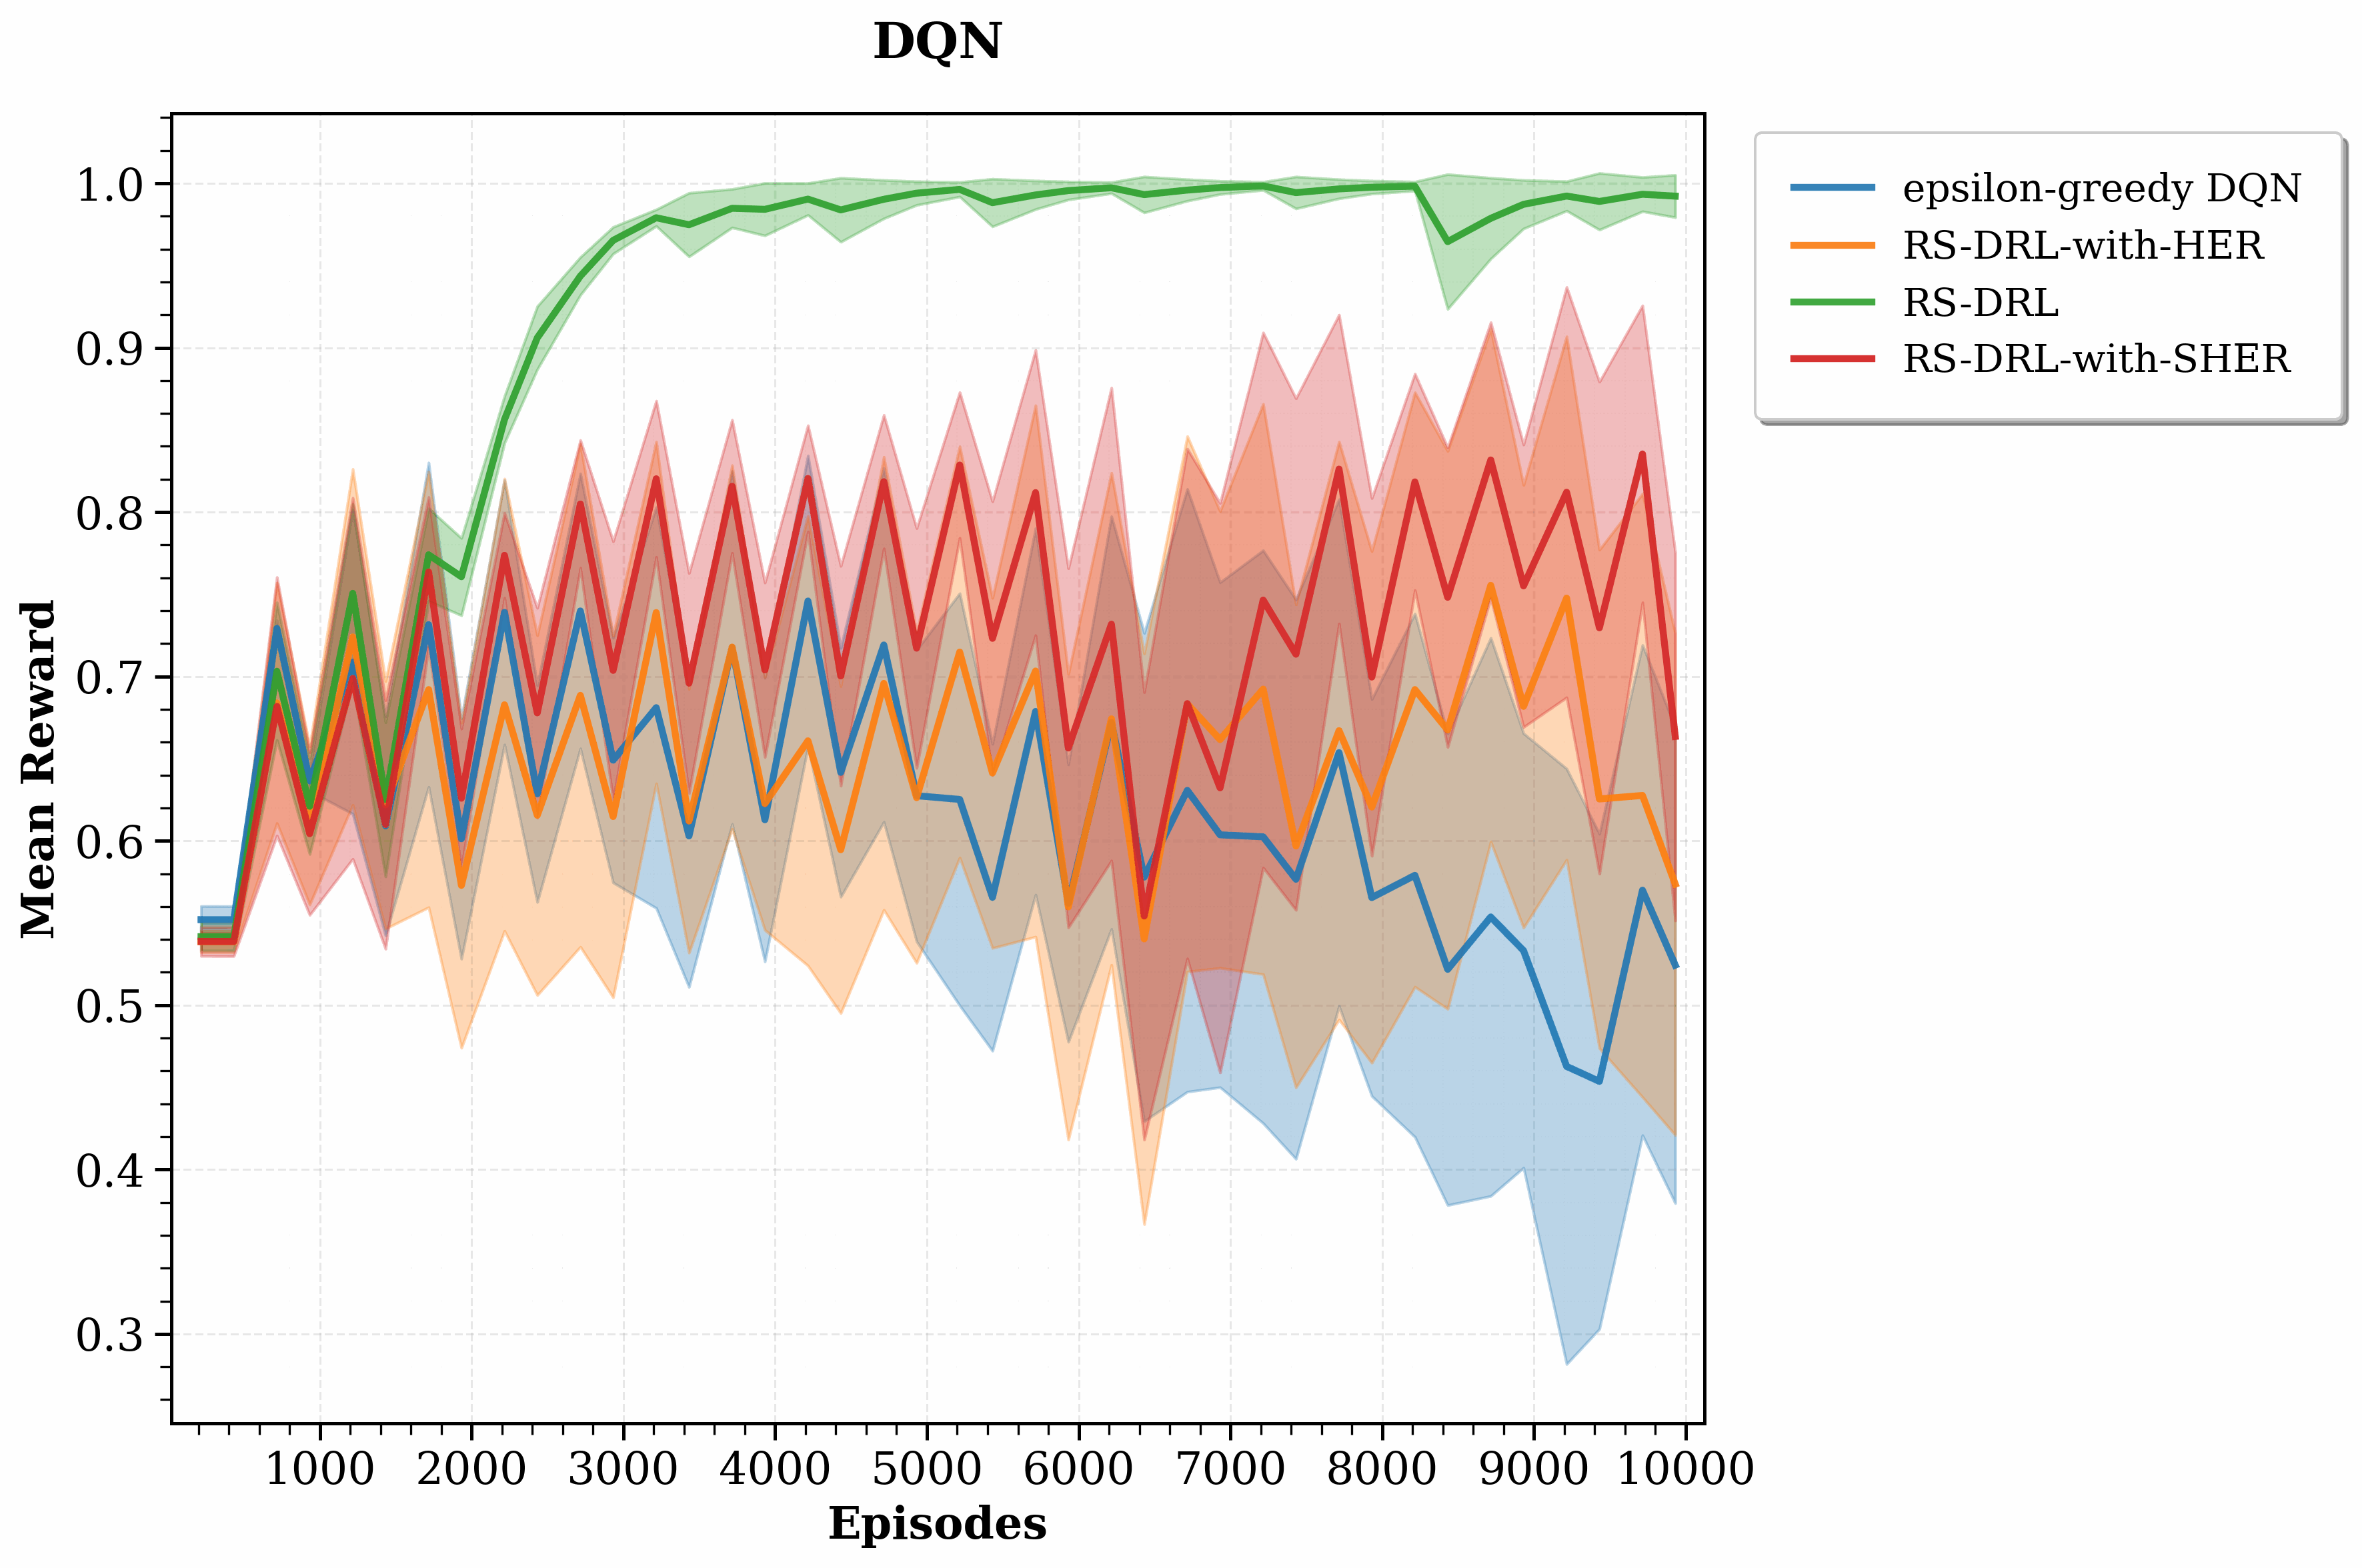
\includegraphics[width=0.7\textwidth]{figures/multiobjective_deltaiotv1.png}
    \caption{منحنی‌های یادگیری الگوریتم‌ها در محیط \lr{DeltaIoTv1} (پاداش در برابر گام‌ها)}
    \label{fig:learning_curve_v1}
\end{figure}

در فضای پیچیده‌تر با حضور ۱۲۹۶ گزینه تطبیق‌پذیر در نسخه \lr{DeltaIoTv1.1}، راهکار پیشنهادی در ۱۹۲۹۶ گام به پاداش $0.8983$ ($\pm 0.0932$) همگرا شد، در حالی که مدل‌های رقیب همگرایی ضعیف‌تری را ثبت کرده و به خط آستانه نرسیدند (مطابق با شکل \ref{fig:learning_curve_v1_1}).

\begin{figure}[htbp]
    \centering
    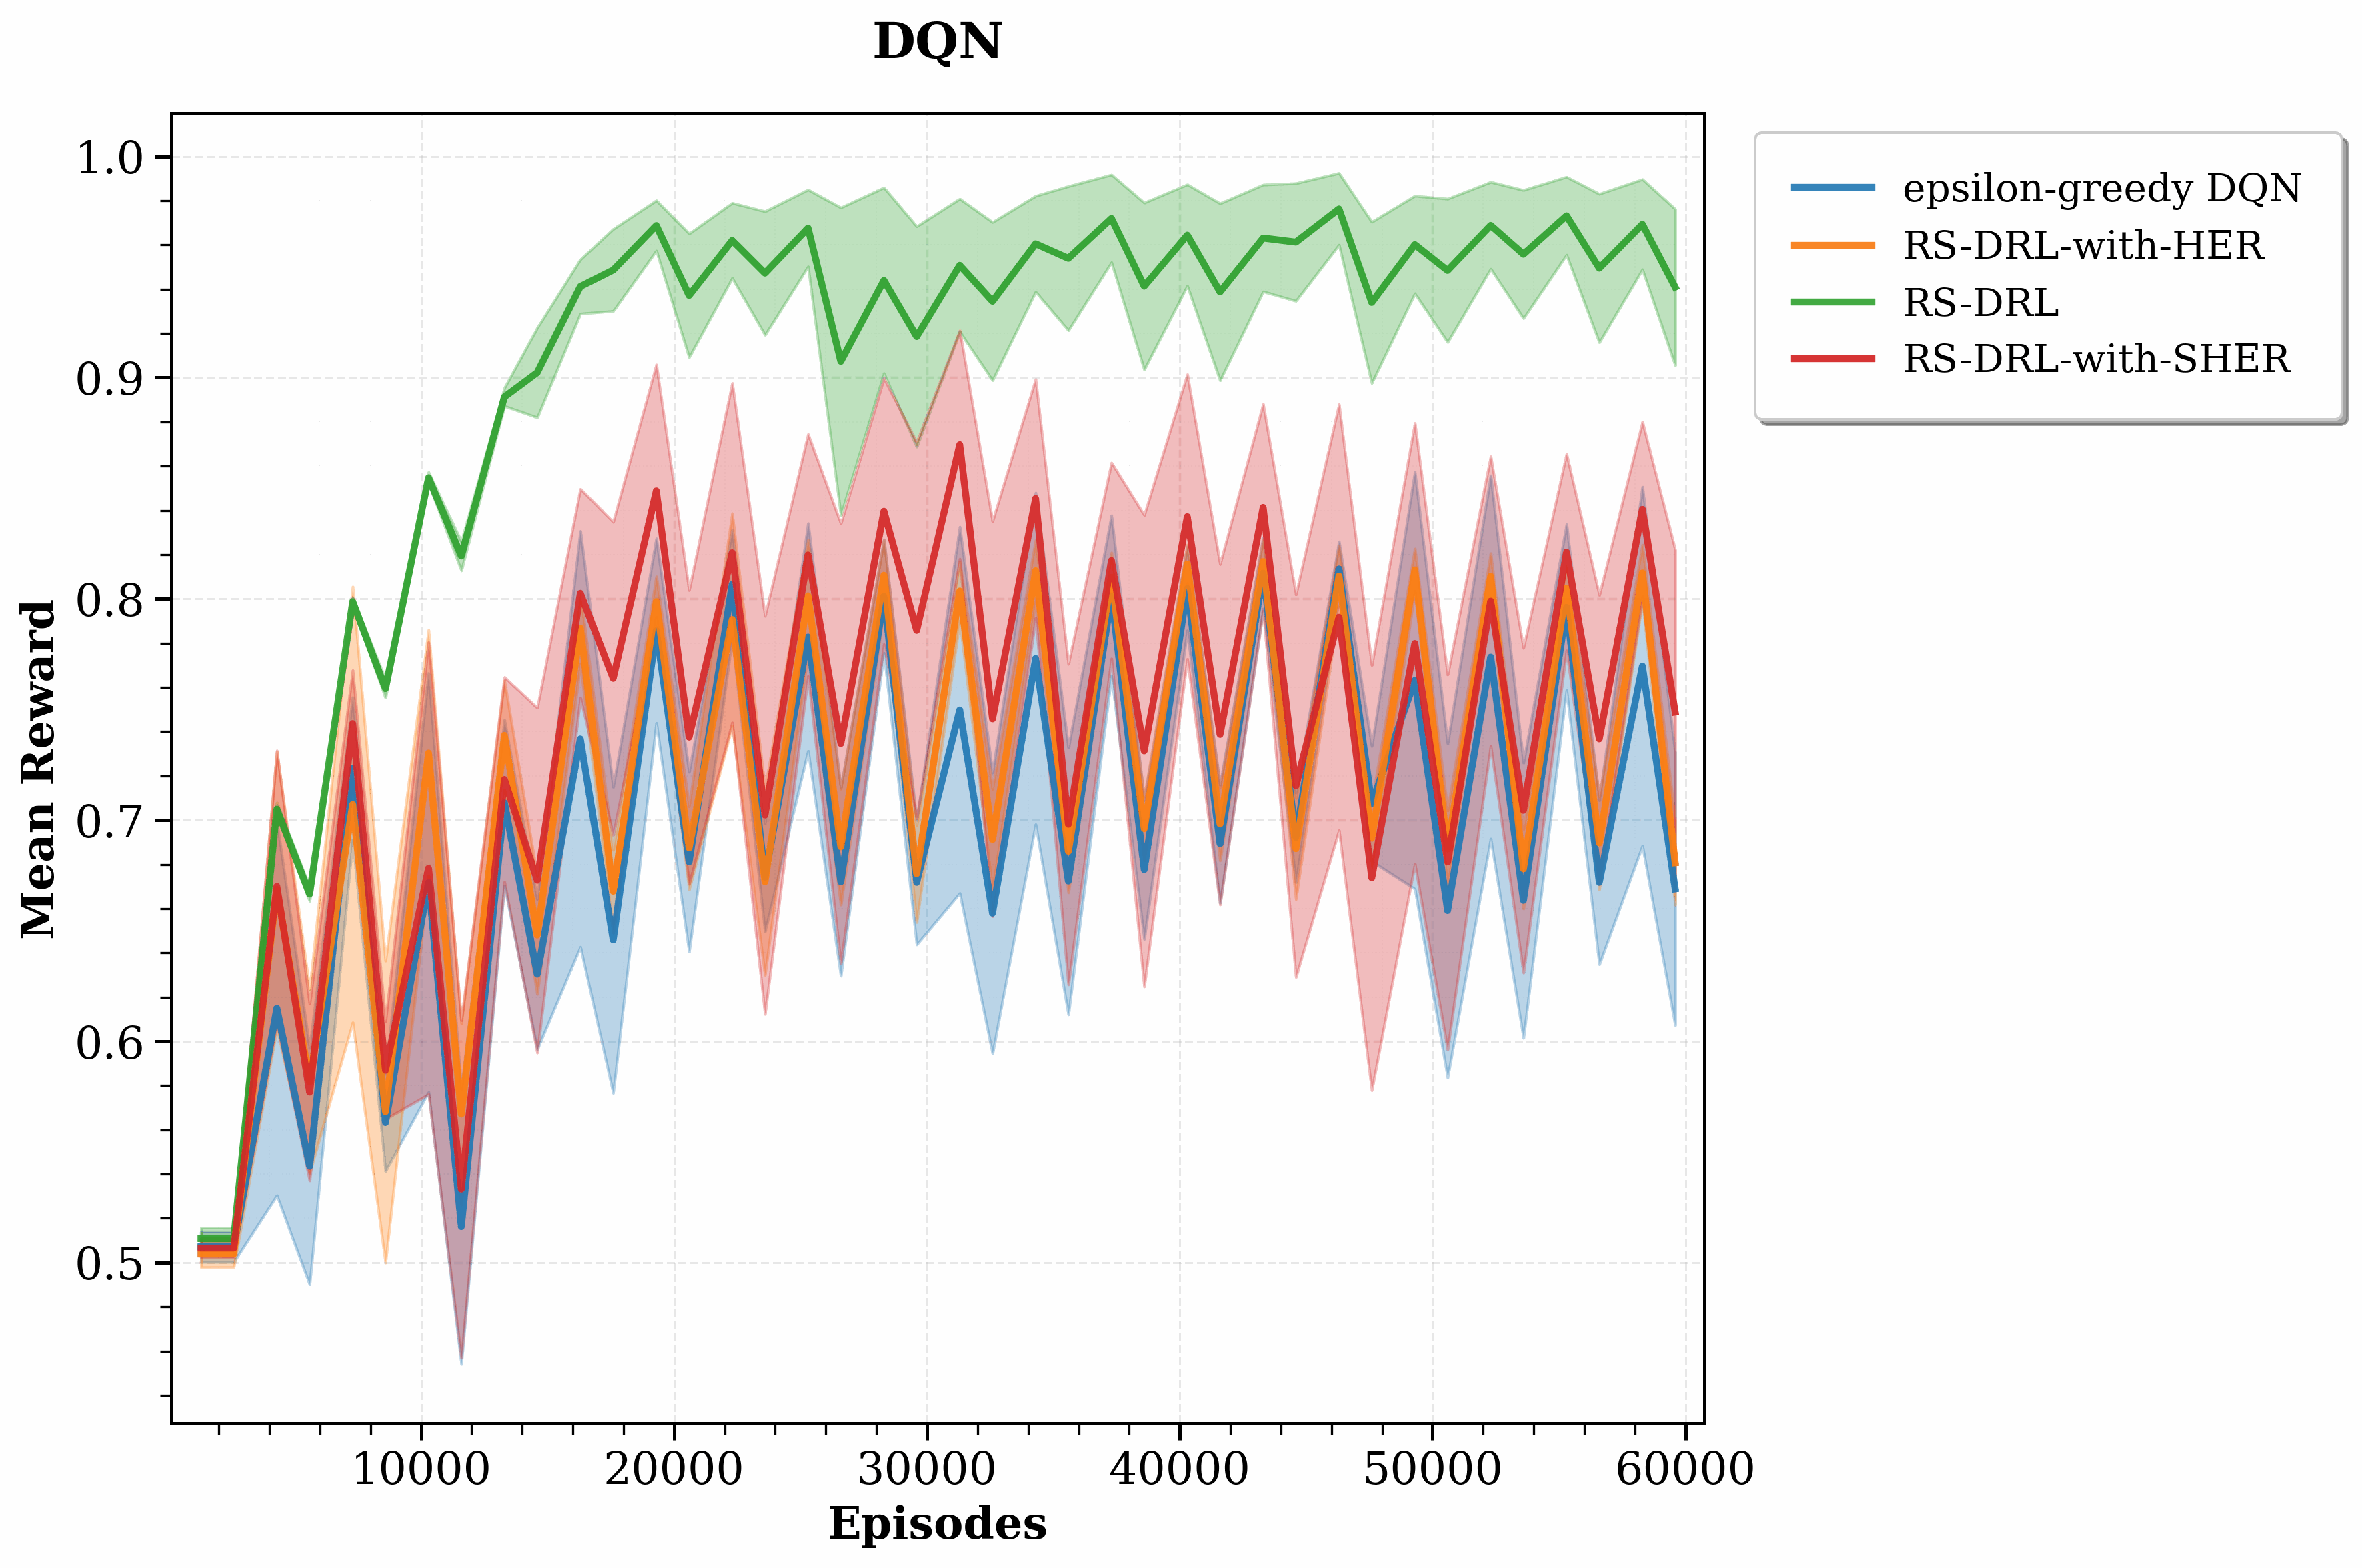
\includegraphics[width=0.7\textwidth]{figures/multiobjective_deltaiotv1.1.png}
    \caption{منحنی‌های یادگیری الگوریتم‌ها در محیط \lr{DeltaIoTv1.1}}
    \label{fig:learning_curve_v1_1}
\end{figure}

\subsection{مقایسه عملکرد به ازای هر هدف و تعمیم‌پذیری (\lr{RQ1} و \lr{RQ2})}

به منظور درک دقیق جزئیات کارکرد عوامل کنترلی روی تک‌تک متغیرهای سیستم، عملکرد رویکرد پیشنهادی در مقایسه با انواع \lr{HER} ارزیابی شد. جداول \ref{tab:min_goals_v1} و \ref{tab:min_goals_v1_1} عملکرد مجانبی، زمان تا آستانه و عملکرد کل را برای اهداف مختلف نشان می‌دهند.

\begin{table}[htbp]
\centering
\caption{نتایج اهداف کمینه‌سازی در \lr{DeltaIoTv1} (پاداش مجانبی / گام‌ها)}
\label{tab:min_goals_v1}
\resizebox{\textwidth}{!}{
\begin{tabular}{|l|ccc|ccc|ccc|}
\hline
\multirow{2}{*}{\textbf{روش}} & \multicolumn{3}{c|}{\textbf{چندهدفه}} & \multicolumn{3}{c|}{\textbf{مصرف انرژی}} & \multicolumn{3}{c|}{\textbf{تلفات بسته‌ها}} \\ \cline{2-10} 
 & \textbf{مجانبی} & \textbf{زمان تا آستانه} & \textbf{عملکرد کل} & \textbf{مجانبی} & \textbf{زمان تا آستانه} & \textbf{عملکرد کل} & \textbf{مجانبی} & \textbf{زمان تا آستانه} & \textbf{عملکرد کل} \\ \hline
\lr{RS-DRL} & \textbf{$\mathbf{0.99}$} & \textbf{2266} & \textbf{--} & \textbf{$\mathbf{0.97}$} & \textbf{--} & \textbf{--} & \textbf{$\mathbf{0.98}$} & \textbf{--} & \textbf{--} \\
\lr{RS-DRL-HER} & $0.61$ & عدم همگرایی & -- & $0.58$ & عدم همگرایی & -- & -- & -- & -- \\
\lr{RS-DRL-SoftHER} & $0.49$ & عدم همگرایی & -- & $0.39$ & عدم همگرایی & -- & -- & -- & -- \\
\lr{DQN} & $0.45$ & عدم همگرایی & -- & -- & عدم همگرایی & -- & -- & -- & -- \\ \hline
\end{tabular}
}
\end{table}

\begin{table}[htbp]
\centering
\caption{نتایج اهداف کمینه‌سازی در \lr{DeltaIoTv1.1}}
\label{tab:min_goals_v1_1}
\resizebox{\textwidth}{!}{
\begin{tabular}{|l|ccc|ccc|ccc|}
\hline
\multirow{2}{*}{\textbf{روش}} & \multicolumn{3}{c|}{\textbf{چندهدفه}} & \multicolumn{3}{c|}{\textbf{مصرف انرژی}} & \multicolumn{3}{c|}{\textbf{تلفات بسته‌ها}} \\ \cline{2-10} 
 & \textbf{مجانبی} & \textbf{زمان تا آستانه} & \textbf{عملکرد کل} & \textbf{مجانبی} & \textbf{زمان تا آستانه} & \textbf{عملکرد کل} & \textbf{مجانبی} & \textbf{زمان تا آستانه} & \textbf{عملکرد کل} \\ \hline
\lr{RS-DRL} & \textbf{$\mathbf{0.89}$} & \textbf{19296} & \textbf{--} & \textbf{$\mathbf{0.93}$} & \textbf{--} & \textbf{--} & \textbf{$\mathbf{0.91}$} & \textbf{--} & \textbf{--} \\
\lr{RS-DRL-HER} & -- & عدم همگرایی & -- & -- & عدم همگرایی & -- & -- & -- & -- \\
\lr{RS-DRL-SoftHER} & -- & عدم همگرایی & -- & -- & عدم همگرایی & -- & -- & -- & -- \\
\lr{DQN} & -- & عدم همگرایی & -- & -- & عدم همگرایی & -- & -- & -- & -- \\ \hline
\end{tabular}
}
\end{table}

شکل \ref{fig:qos_profiles_deltaiotv1} رفتار زمانی شاخص‌های سه‌گانه کیفیت خدمات شامل نرخ اتلاف بسته، تأخیر انتقال پیام و مصرف کل انرژی را در طول دوره‌های انطباق در بستر \lr{DeltaIoTv1} نشان می‌دهد.

\begin{figure}[htbp]
\centering
\subfigure[نرخ اتلاف بسته]{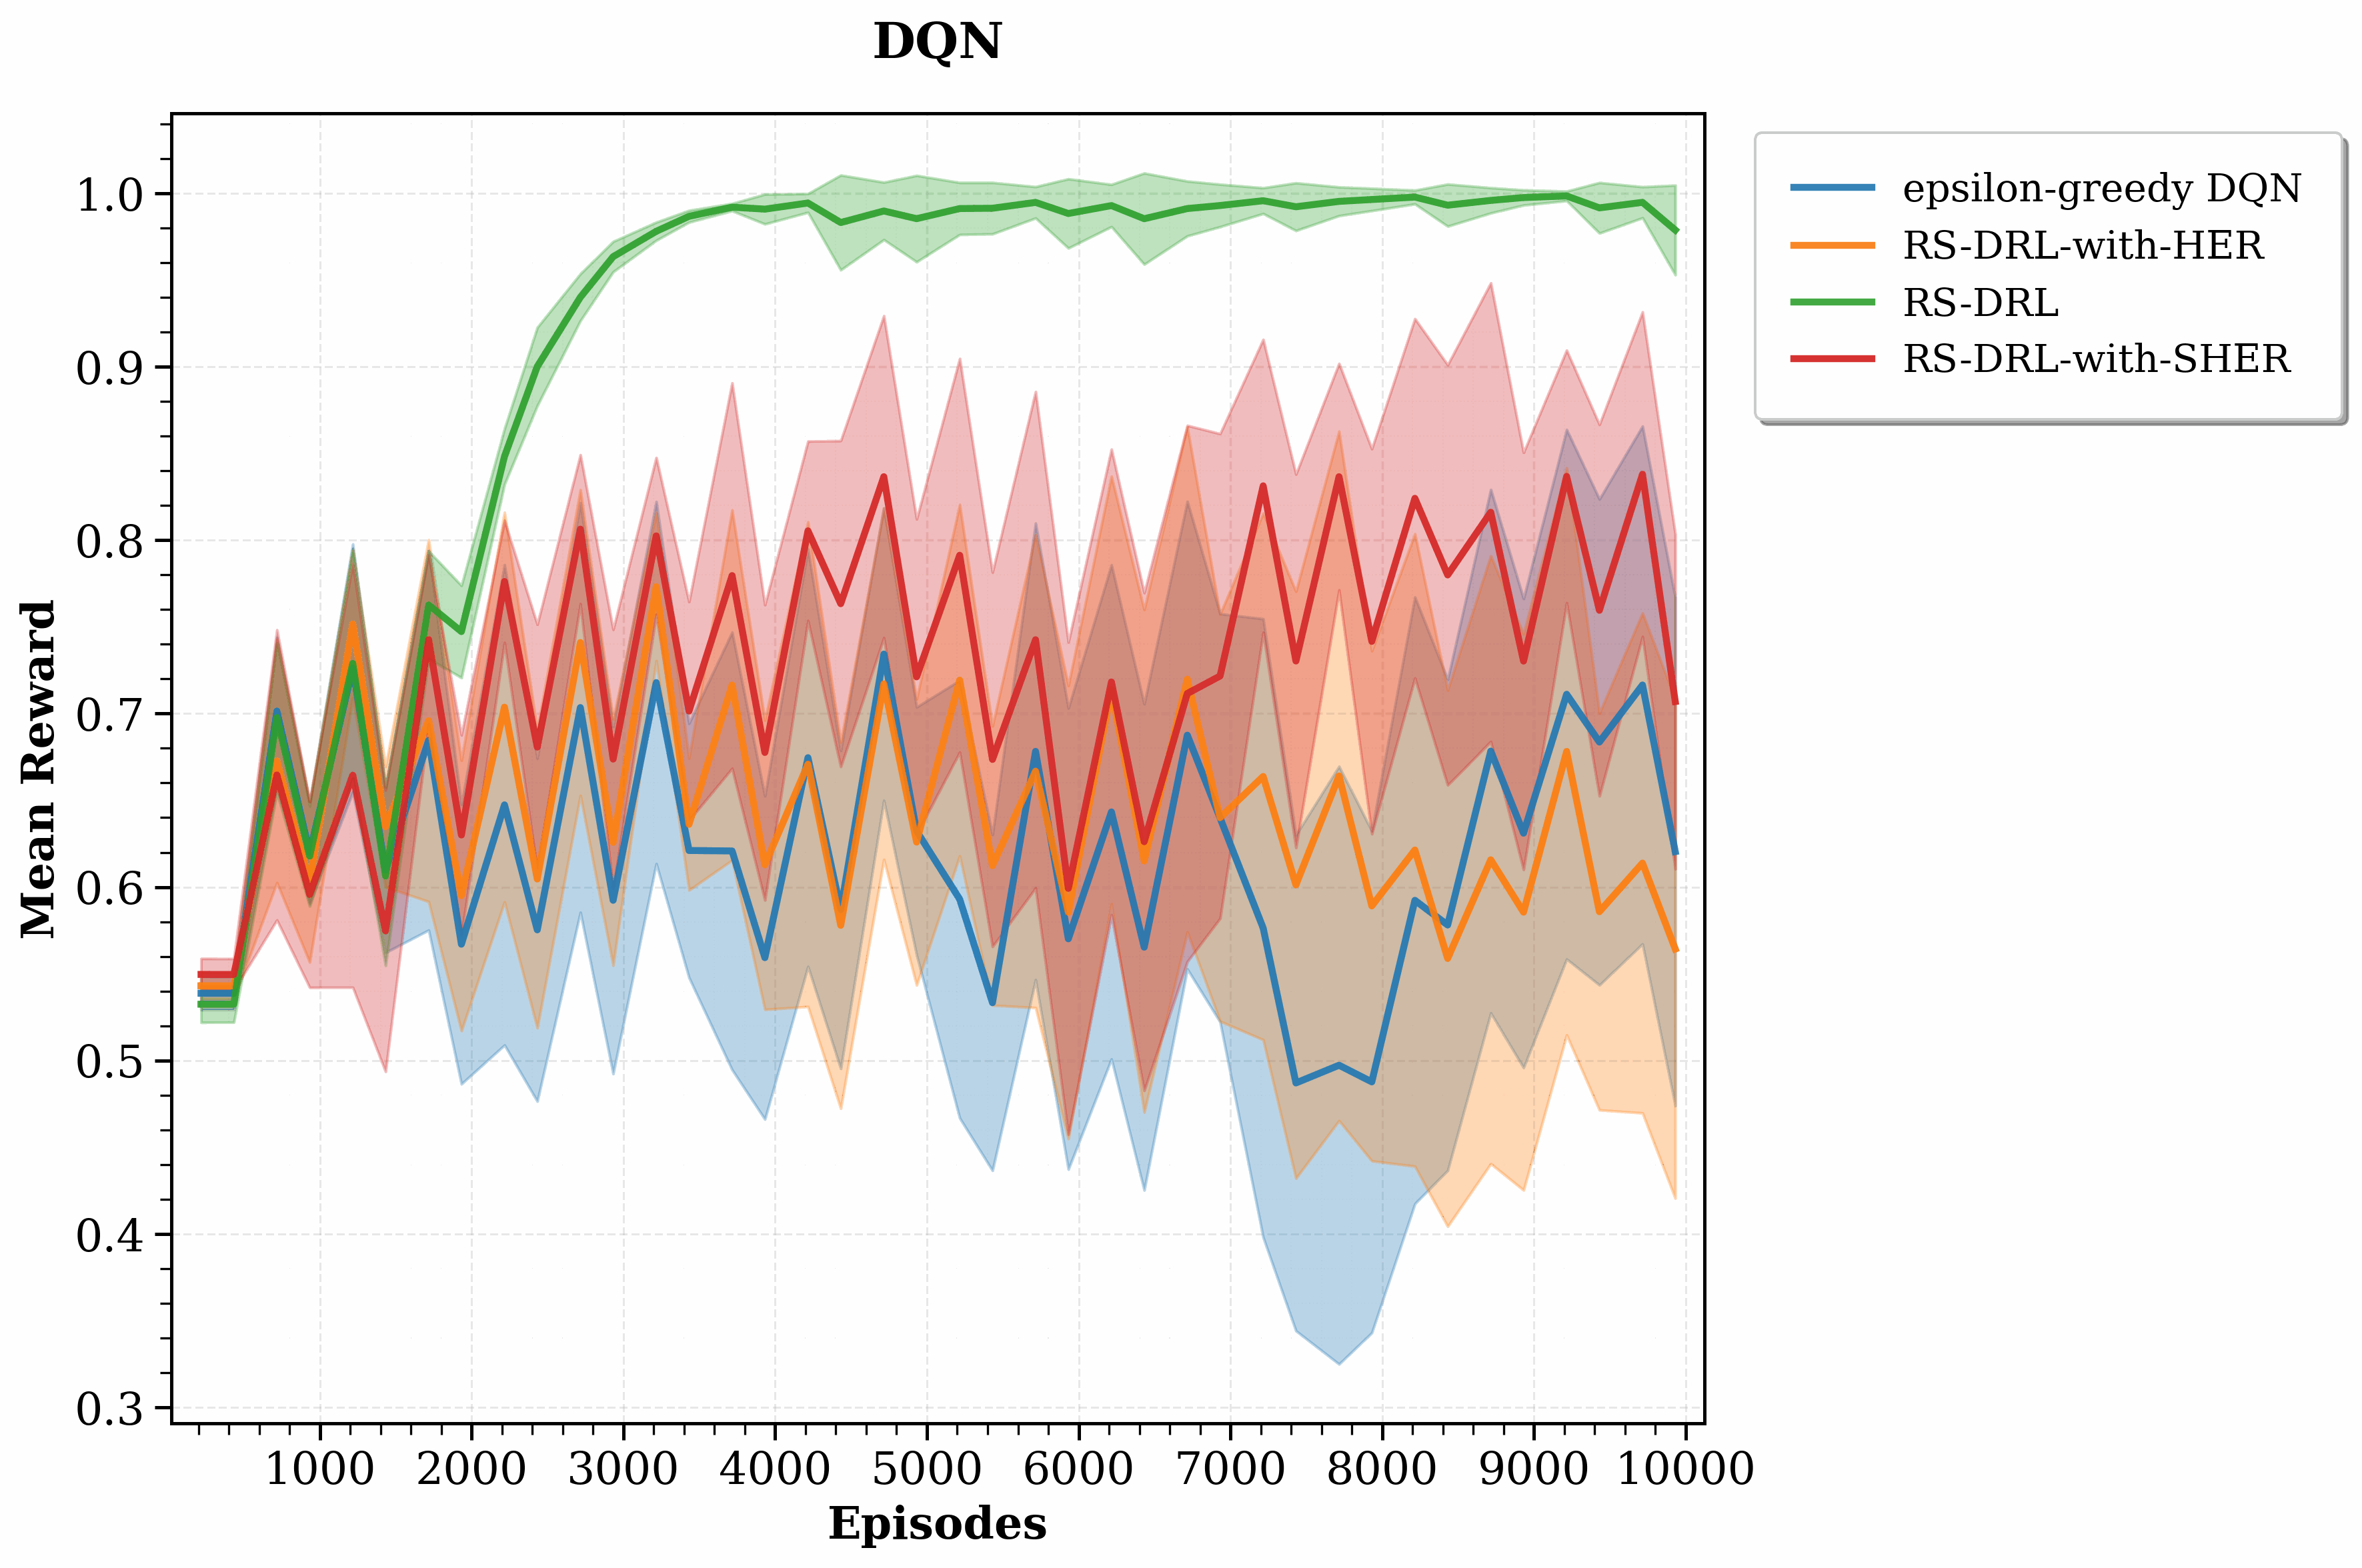
\includegraphics[width=0.32\textwidth]{figures/packetloss_deltaiotv1.png}\label{fig:sub_packetloss}}
\hfill
\subfigure[تأخیر انتقال پیام]{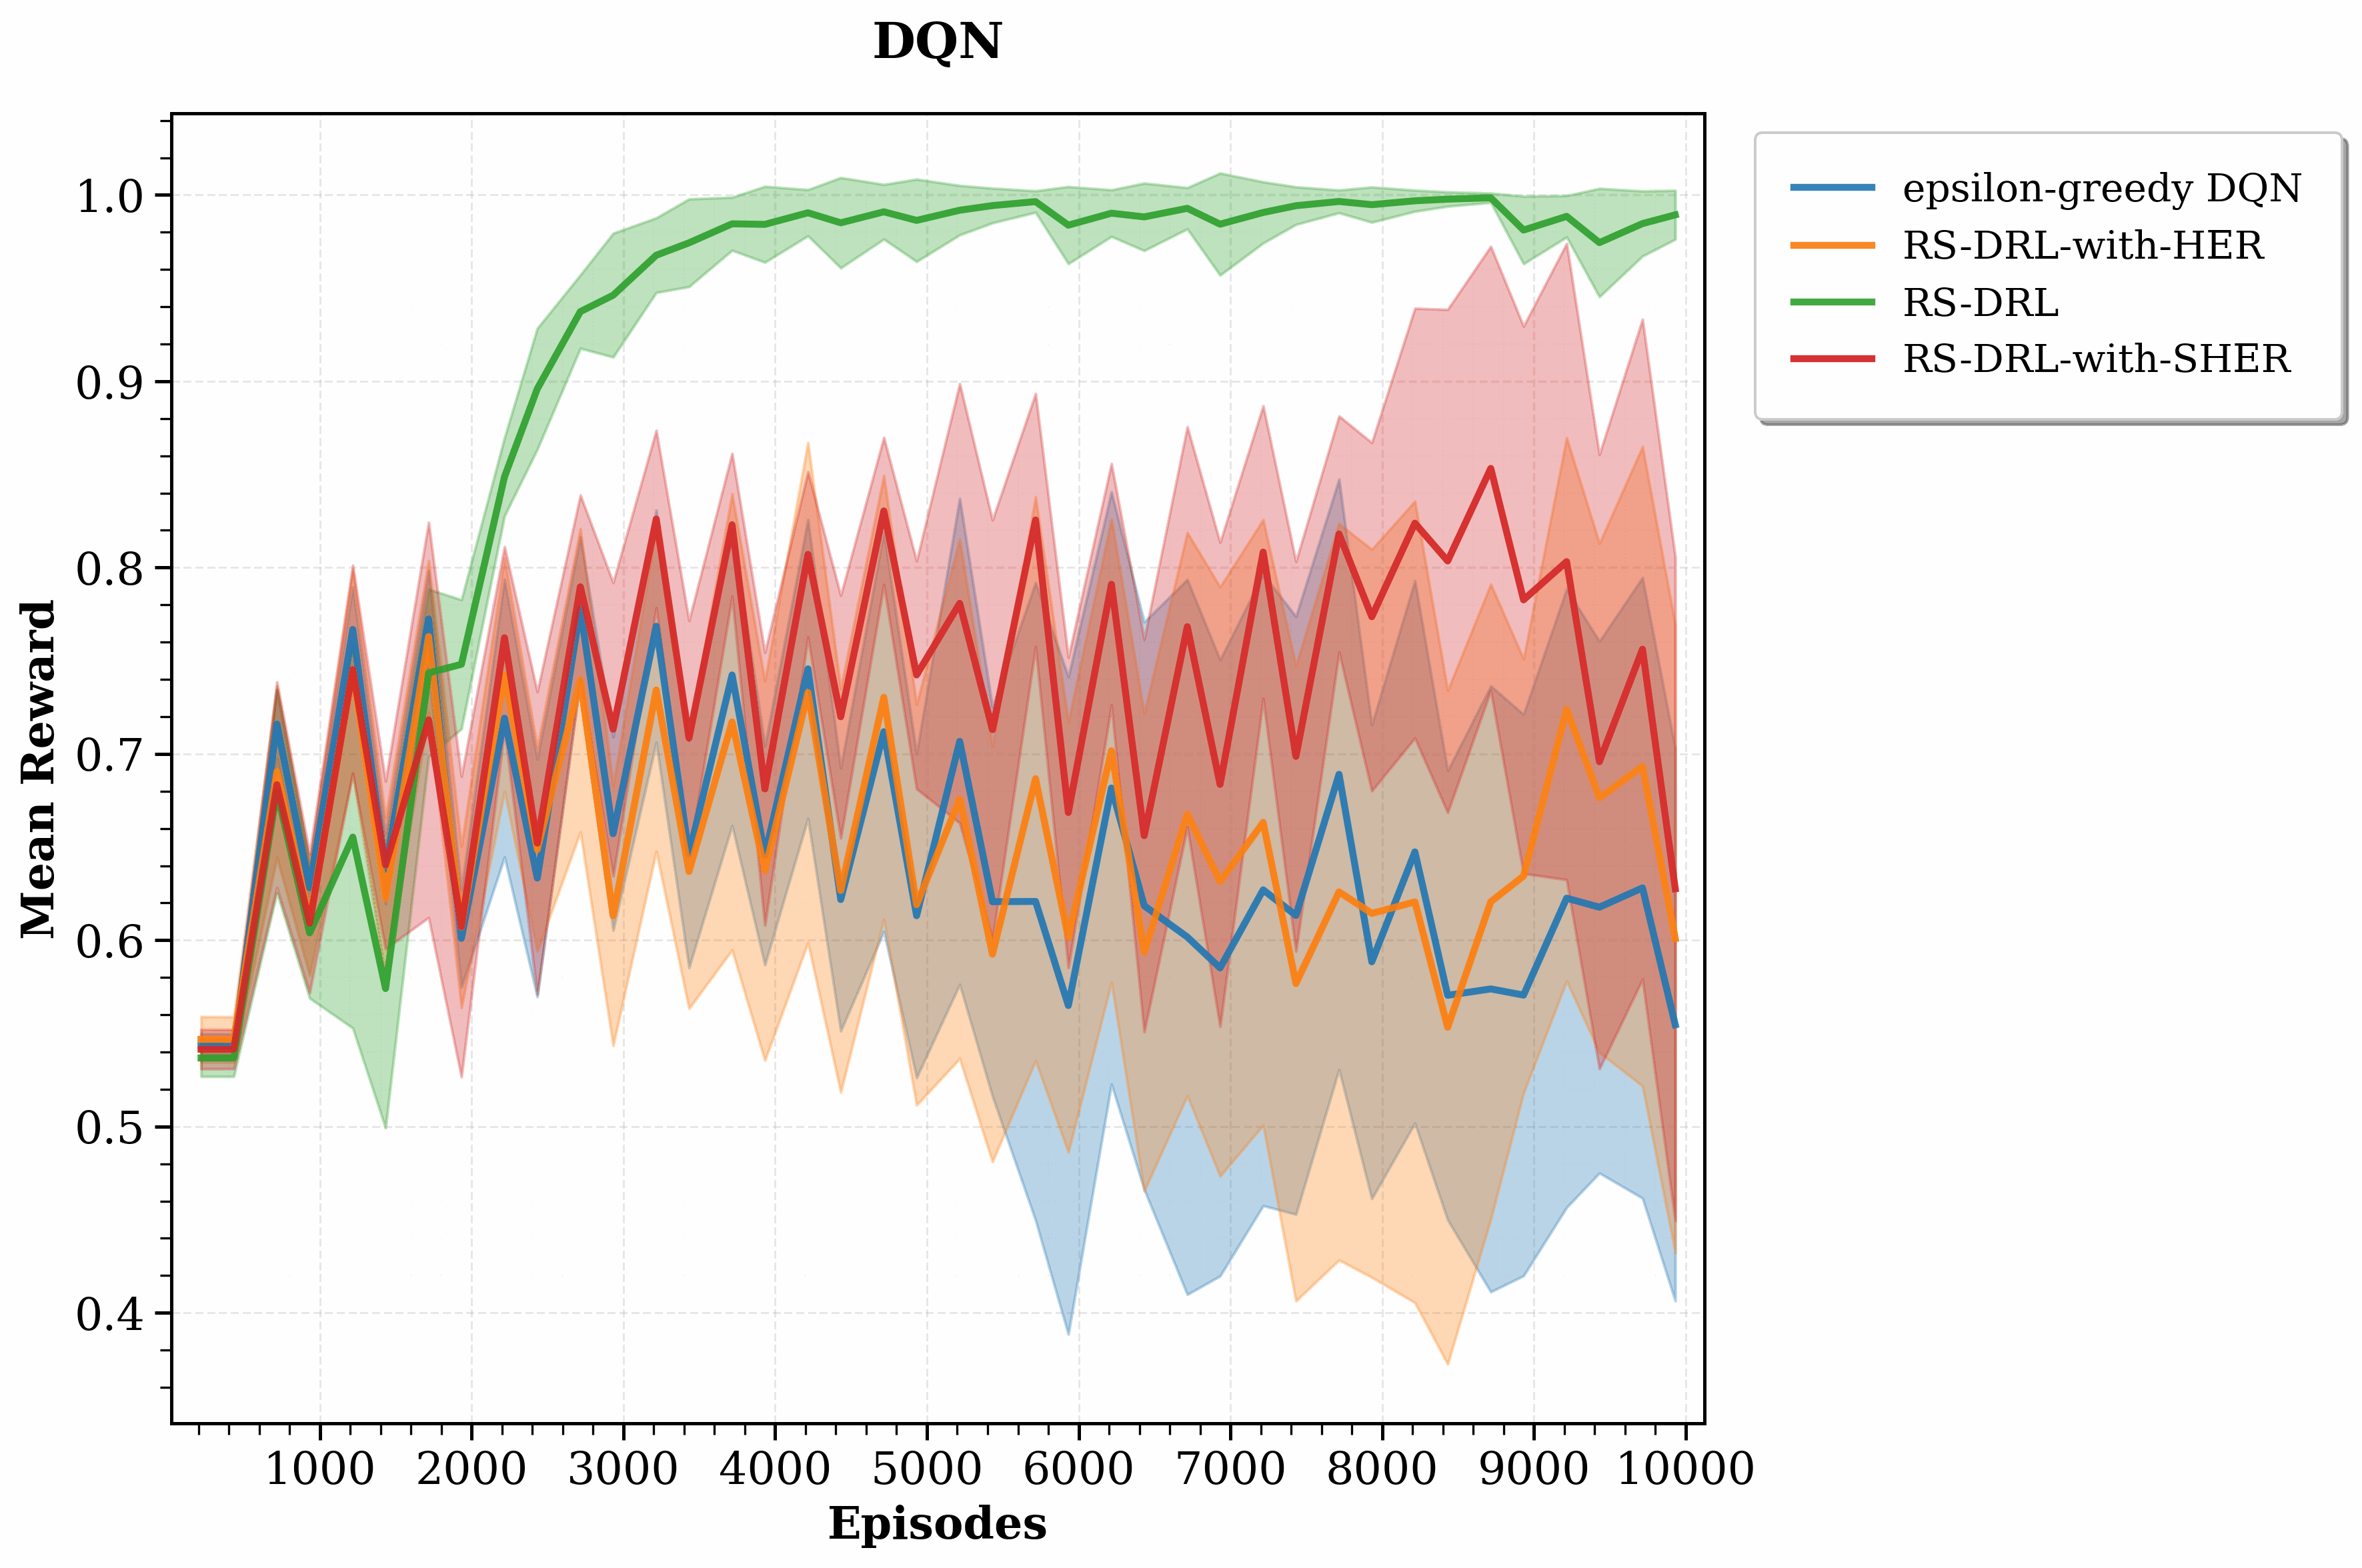
\includegraphics[width=0.32\textwidth]{figures/latency_deltaiotv1.png}\label{fig:sub_latency}}
\hfill
\subfigure[مصرف انرژی گره‌ها]{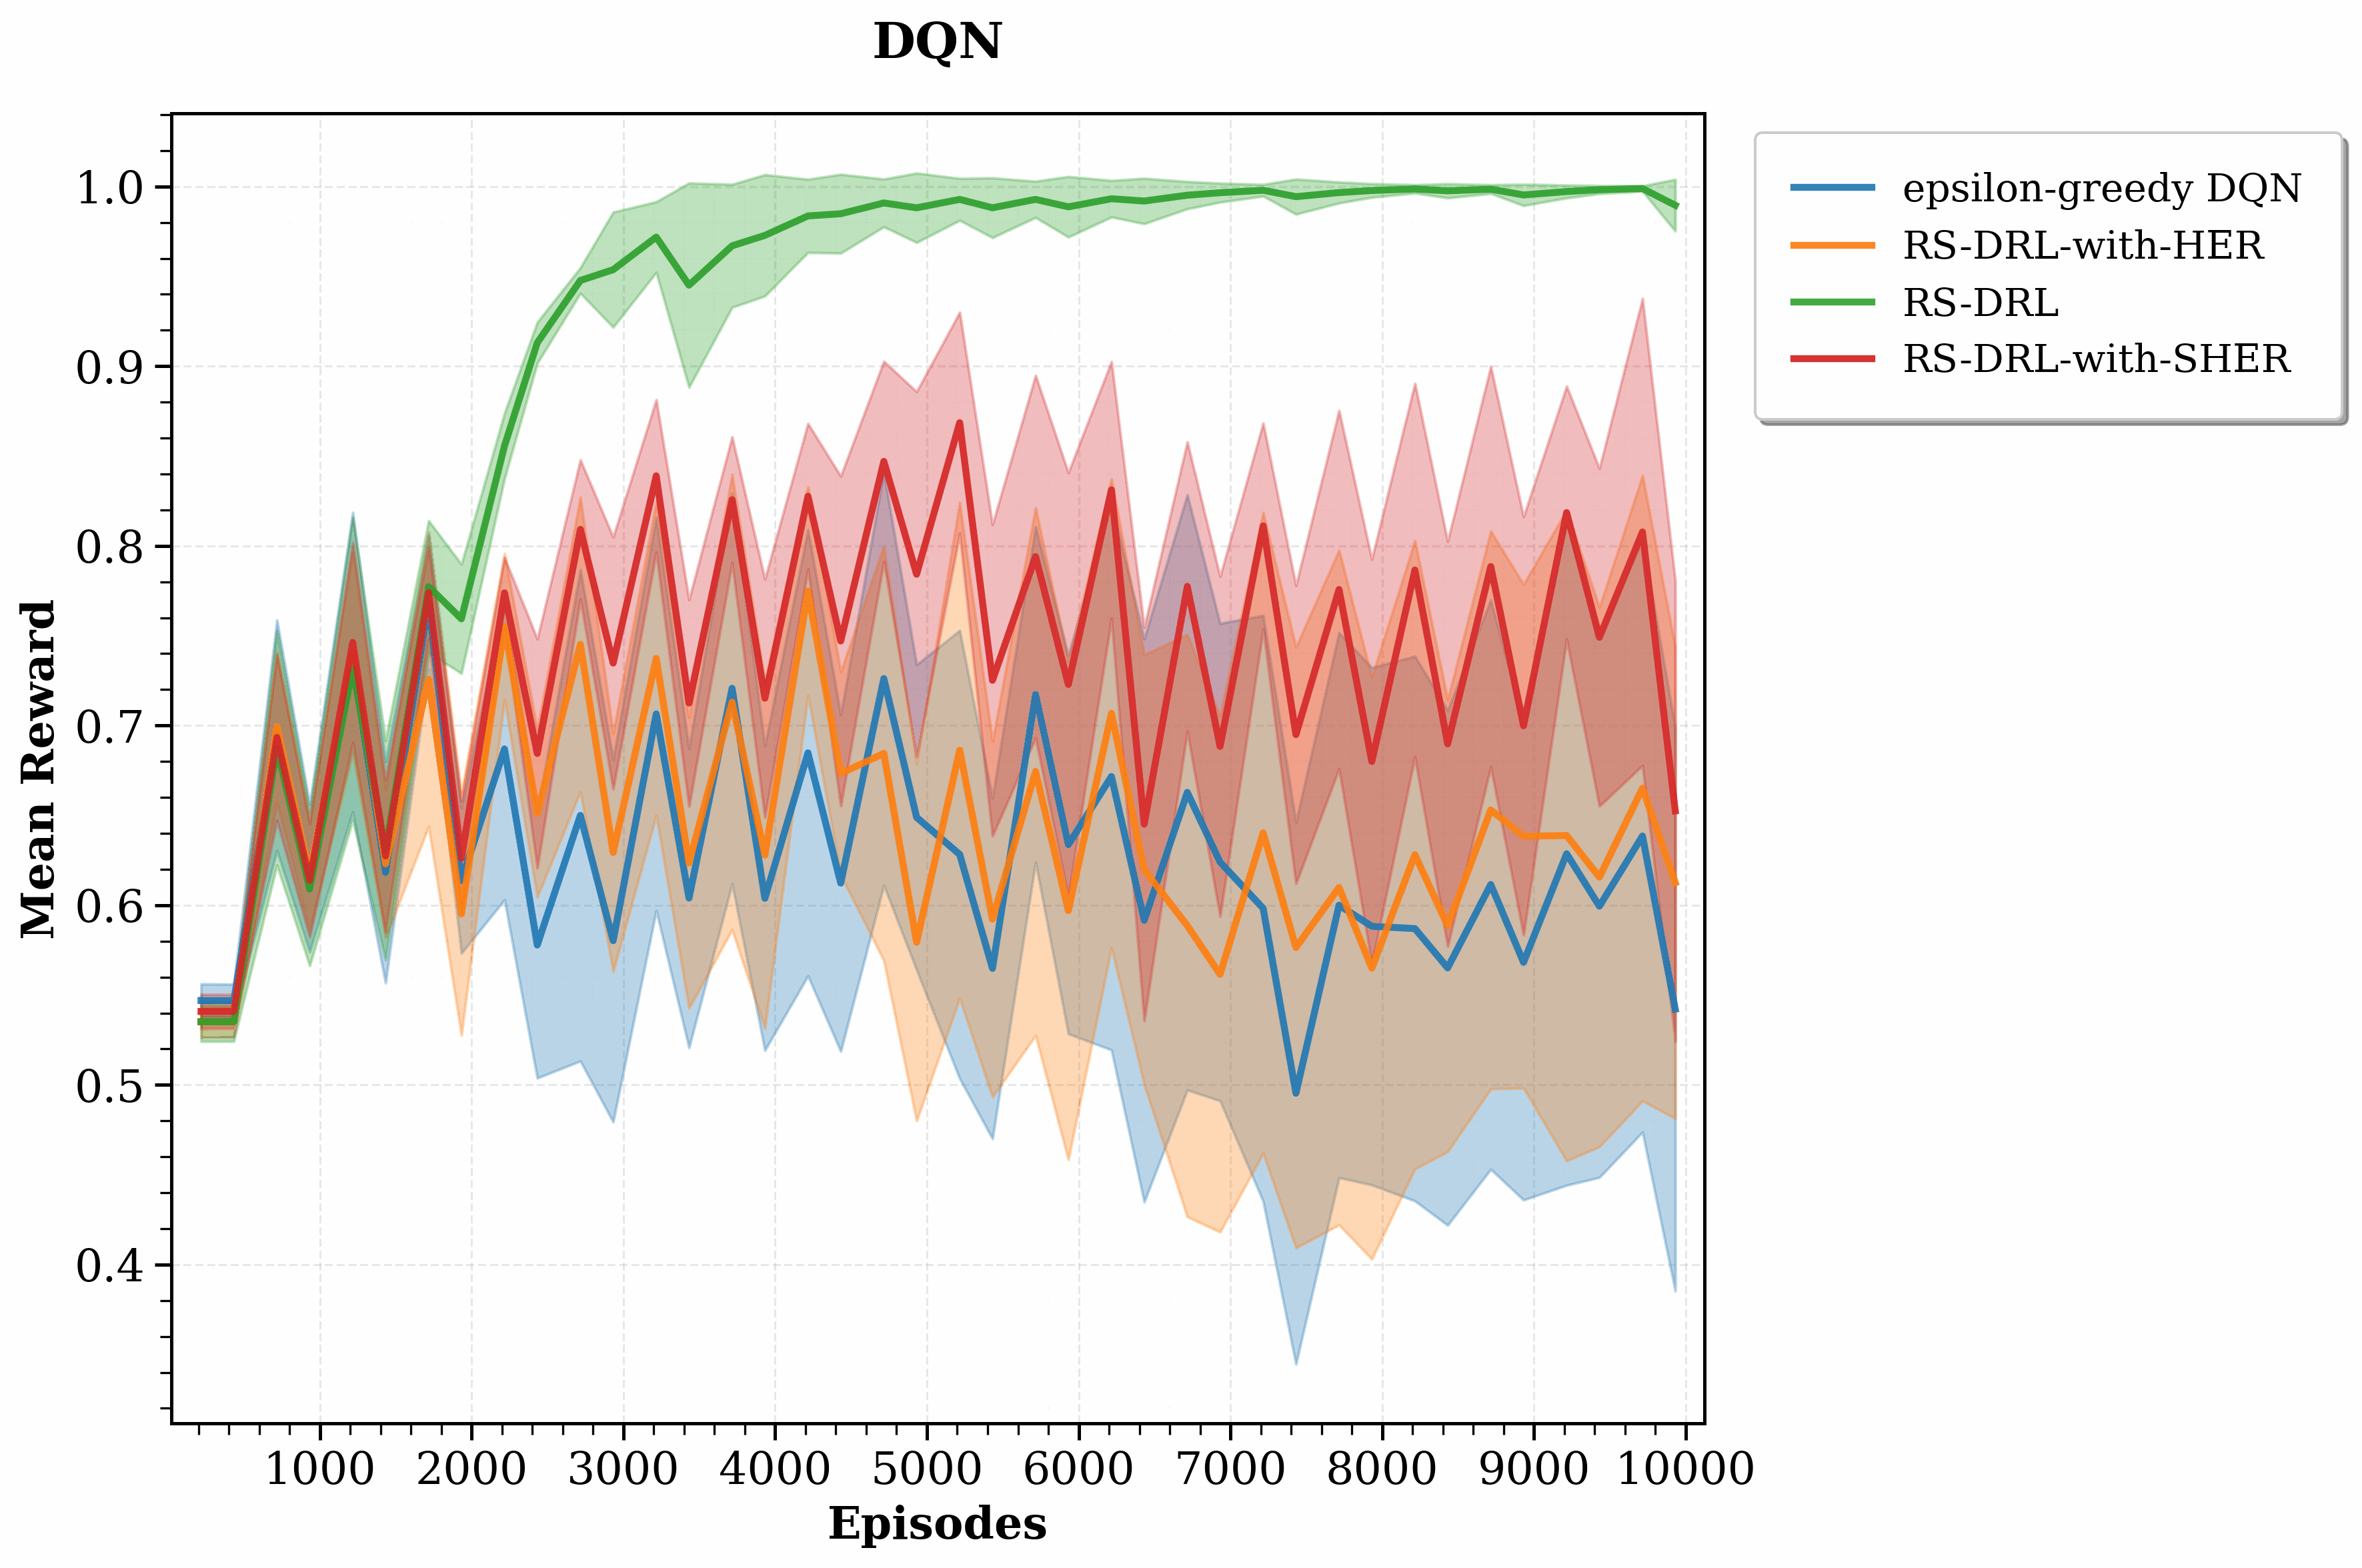
\includegraphics[width=0.32\textwidth]{figures/energy_consumption_deltaiotv1.png}\label{fig:sub_energy}}
\caption{پروفایل زمانی شاخص‌های سه‌گانه کیفیت خدمات در طول دوره‌های انطباق در بستر \lr{DeltaIoTv1}: مقایسه روش پیشنهادی \lr{RS-DRL} با روش‌های خط پایه.}
\label{fig:qos_profiles_deltaiotv1}
\end{figure}

تحلیل این اهداف نشان می‌دهد:
\begin{itemize}
  \item \textbf{بهینه‌سازی چندهدفه:}\LTRfootnote{Multi-objective} رویکرد پیشنهادی به پاداش میانگین $0.9905$ (در نسخه اول) و $0.8983$ (در نسخه دوم) دست یافت، در حالی که روش‌های مبتنی بر \lr{HER} به دلیل ماهیت وابسته به اهداف صریح، در بازه $0.49$ تا $0.61$ متوقف شدند.
  \item \textbf{مصرف انرژی:} شاخص‌های ارزیابی، پاداش مصرف انرژی \lr{RS-DRL} را با ثبت میانگین $0.9756$ (در \lr{v1}) و $0.9301$ (در \lr{v1.1}) بسیار مطلوب‌تر از مدل‌های پایه (بازه $0.39$ تا $0.58$) نشان داد.
  \item \textbf{تلفات بسته‌ها:} پاداش متناظر با نرخ اتلاف بسته‌ها برای روش پیشنهادی برابر با $0.9850$ در شبکه اول و $0.9129$ در شبکه دوم حاصل گردید که بیانگر پایداری کیفیت خدمات شبکه در شرایط نویزی است.
  \item \textbf{تأخیر ارسال:} روش پیشنهادی \lr{RS-DRL} با میانگین پاداش $0.9964$ در نسخه اول و $0.9021$ در نسخه دوم، کمترین تأخیر انتقال پیام را در مقایسه با رقبا ثبت نمود.
\end{itemize}

\subsection{ارزیابی مقایسه‌ای در برابر تمام روش‌های پایه (\lr{RQ4})}

ارزیابی شبکه در تقابل با دیگر رقبا نظیر روش‌های جستجوگر، اهمیت ویژه‌ای دارد. در جداول \ref{tab:tts_goals} و \ref{tab:tt_goals} نتایج مربوط به اهداف آستانه‌ای خلاصه شده است.

\begin{table}[htbp]
\centering
\caption{عملکرد سیستم برای اهداف آستانه‌ای ترکیبی \lr{TTS}}
\label{tab:tts_goals}
\begin{tabular}{|l|ccc|}
\hline
\textbf{روش (شبکه \lr{v1})} & \textbf{اتلاف بسته‌ها (\%)} & \textbf{تاخیر (\lr{s})} & \textbf{مصرف انرژی (\lr{C})} \\ \hline
\lr{RS-DRL} & \textbf{$\mathbf{10.578}$} & \textbf{$\mathbf{0.097}$} & $12.882$ \\ 
\lr{DLASER+} & $12.890$ & $0.840$ & $13.020$ \\ 
\lr{Reference} & $14.230$ & $0.100$ & $13.100$ \\ \hline
\end{tabular}
\end{table}

\begin{table}[htbp]
\centering
\caption{عملکرد سیستم برای اهداف آستانه‌ای مطلق \lr{TT}}
\label{tab:tt_goals}
\begin{tabular}{|l|c|c|c|c|}
\hline
\multirow{2}{*}{\textbf{روش}} & \multicolumn{2}{c|}{\textbf{\lr{DeltaIoTv1}}} & \multicolumn{2}{c|}{\textbf{\lr{DeltaIoTv2}}} \\ \cline{2-5}
 & \textbf{اتلاف بسته‌ها (\%)} & \textbf{تاخیر (\lr{s})} & \textbf{اتلاف بسته‌ها (\%)} & \textbf{تاخیر (\lr{s})} \\ \hline
\lr{RS-DRL} & \textbf{$\mathbf{7.153}$} & -- & \textbf{$\mathbf{9.330}$} & $0.251$ \\
\lr{DLASER+} & $7.980$ & -- & -- & -- \\
\lr{ML4EAS} & -- & -- & $10.560$ & -- \\
\lr{Reference} & -- & -- & -- & \textbf{$\mathbf{0.100}$} \\ \hline
\end{tabular}
\end{table}

در خصوص \textbf{هدف ترکیبی \lr{TTS}} در نسخه اول شبکه، روش \lr{RS-DRL} نرخ اتلاف بسته را به $10.578\%$ محدود ساخت؛ در حالی که روش جستجوی مرجع دارای اتلاف $14.230\%$ و روش \lr{DLASER+} دارای اتلاف $12.890\%$ بوده‌اند. تأخیر ارسال نیز با ثبت مقدار $0.097\,\text{s}$ به طور قابل‌ملاحظه‌ای کمتر از \lr{DLASER+} ($0.840\,\text{s}$) بوده و با روش مرجع ($0.100\,\text{s}$) برابری می‌کند. همچنین مصرف انرژی ($12.882\,\text{C}$) در سطحی کاملاً رقابتی و مشابه روش‌های مرجع ($13.100\,\text{C}$) و \lr{DLASER+} ($13.020\,\text{C}$) حفظ گردید.

در مقابل، در \textbf{هدف آستانه‌ای مطلق \lr{TT}}، سیاست پیشنهادی در بستر \lr{DeltaIoTv1} به نرخ اتلاف $7.153\%$ (در برابر $7.980\%$ در \lr{DLASER+}) دست یافت. علاوه بر این، در نسخه مقیاس‌بزرگ \lr{DeltaIoTv2}، مقدار اتلاف بسته به $9.330\%$ مقید گردید که در مقایسه با روش \lr{ML4EAS} ($10.560\%$) بهبود محسوسی را نشان می‌دهد.

در شاخص تأخیر نسخه دوم، روش \lr{RS-DRL} مقدار $0.251\,\text{s}$ را در برابر $0.100\,\text{s}$ روش مرجع ثبت نمود؛ این رفتار ناشی از مصالحه چندهدفه و اولویت‌بخشی سیاست یادگیری به کاهش اتلاف بسته در شرایط بار ترافیکی شدید شبکه است.

\subsection{مطالعه تفکیک اثر و ابلیشن: حساسیت به ضریب شکل‌دهی \texorpdfstring{$\rho$}{ρ} (\lr{RQ2})}
\label{subsec:ablation_rho}

پارامتر $\rho$ (ضریب شکل‌دهی) شدت خوش‌بینی عامل را در بازطراحی تجربیات ناموفق کنترل می‌کند. این پارامتر مشخص می‌سازد که چه نسبتی از تجربیات با پاداش صفر در هر دسته نمونه‌برداری‌شده از بافر بازپخش، با پاداش مثبت خوش‌بینانه ($\tilde{r} = 1$) جایگزین شوند.
جهت تحلیل تجربی، اثر مقادیر مختلف $\rho$ در قالب شکل \ref{fig:ablation_rho} ارزیابی شده است.

\begin{figure}[htbp]
    \centering
    \includegraphics[width=0.7\textwidth]{figures/ablation_rho.pdf}
    \caption{تاثیر مقادیر مختلف ضریب شکل‌دهی $\rho$ بر پاداش مجانبی و عملکرد کل}
    \label{fig:ablation_rho}
\end{figure}

\textbf{نکات تحلیلی پیرامون ضریب شکل‌دهی $\rho$:}
ایجاد توازن دقیق در انتخاب مقدار ضریب $\rho$ ضروری است: مقادیر بیش از حد بزرگ ($\rho > 0.6$)، منجر به تزریق مفرط پاداش‌های مثبت تصنعی و نوسان شدید در برآورد گرادیان شده و همگرایی را ناپایدار می‌سازد. در مقابل، مقادیر بسیار کوچک ($\rho < 0.2$) انگیزه کافی برای کاوش حالت‌های ناشناخته ایجاد نکرده و عامل مشابه روش‌های یادگیری بدون هدایت در اولین بهینه محلی متوقف می‌شود. مقدار بهینه $\rho = 0.3$ علاوه بر تسریع همگرایی، از بیش‌برازش\LTRfootnote{Overfitting} بر روی تجربیات پیشین بافر بازپخش جلوگیری می‌کند. جدول \ref{tab:rho_sensitivity} تاثیر مقادیر مختلف این پارامتر را بر روی رفتار کاوش، پایداری و فرار از بهینه‌های محلی بر مبنای جستجوی شبکه‌ای خلاصه می‌کند.

\begin{table}[htbp]
\centering
\caption{تحلیل تجربی حساسیت رفتار یادگیری عامل نسبت به تغییرات ضریب شکل‌دهی $\rho$}
\label{tab:rho_sensitivity}
\resizebox{\textwidth}{!}{%
\begin{tabular}{|c|c|c|p{7cm}|}
\hline
\textbf{مقدار $\rho$} & \textbf{نرخ کاوش} & \textbf{پایداری همگرایی} & \textbf{تاثیر بر فرار از بهینه محلی} \\ \hline
$0.0$ & بسیار پایین & بسیار بالا & فاقد توانایی فرار؛ عامل همواره در اولین بهینه محلی یافت شده متوقف می‌شود. \\ \hline
$0.1$ & متوسط & بالا & شروع فرار تدریجی؛ زمان طولانی‌تری برای همگرایی به بهینه مطلق نیاز دارد. \\ \hline
$0.3$ & بهینه تجربی & پایدار & فرار سریع و پایدار؛ توازن بهینه میان کاوش خوش‌بینانه و همگرایی مجانبی. \\ \hline
$0.7$ & بالا & متوسط (نوسانی) & القای نویز به گرادیان سیاست و بروز نوسان در روند همگرایی مجانبی. \\ \hline
$0.9$ & بیش‌کاوشی مفرط & ناپایدار & ناپایداری شدید؛ واگرایی سیاست یادگیری ناشی از تزریق بیش از حد پاداش‌های مصنوعی. \\ \hline
\end{tabular}%
}
\end{table}

\subsection{ارزیابی ماژول اعتبارسنجی صوری ناهمگام \lr{UPPAAL-SMC} و کران چرنوف (\lr{RQ5})}
\label{subsec:uppaal_smc_eval}

برای اعتبارسنجی تجربی ماژول اعتبارسنجی صوری ناهمگام معرفی‌شده در بخش \ref{sec:formal_verification_sec}، مدل شبکه حسگر \lr{DeltaIoT} در ابزار وارسی مدل آماری \lr{UPPAAL-SMC} بارگذاری گردید. مشخصه‌های کیفی شبکه در قالب منطق زمانی درخت محاسباتی احتمالی (\lr{PCTL}) فرمول‌بندی شده و پارامترهای آماری بر پایه سطح اطمینان ۹۵٪ ($\alpha = 0.05$) و حاشیه خطای $\delta = 0.02$ تنظیم شدند. طبق قضیه کران چرنوف-هوفدینگ (معادله \ref{eq:chernoff_bound} در فصل ۴)، حداقل تعداد شبیه‌سازی‌های تصادفی مونت‌کارلو برای تضمین این سطح از دقت برابر است با:
\begin{equation}
\label{eq:chernoff_eval_bound}
N_{\text{sim}} \ge \frac{\ln(2/\alpha)}{2\delta^2} = \frac{\ln(2/0.05)}{2(0.02)^2} = \frac{3.6888}{0.0008} \approx 4611
\end{equation}

شکل \ref{fig:ch5_chernoff_sample_bound} تحلیل تحلیلی کران چرنوف-هوفدینگ و تعداد شبیه‌سازی‌های موردنیاز را در سطوح مختلف اطمینان ($1-\alpha \in [0.90, 0.99]$) و حاشیه‌های خطای مجاز ($\delta$) نشان می‌دهد.

\begin{figure}[htbp]
\centering
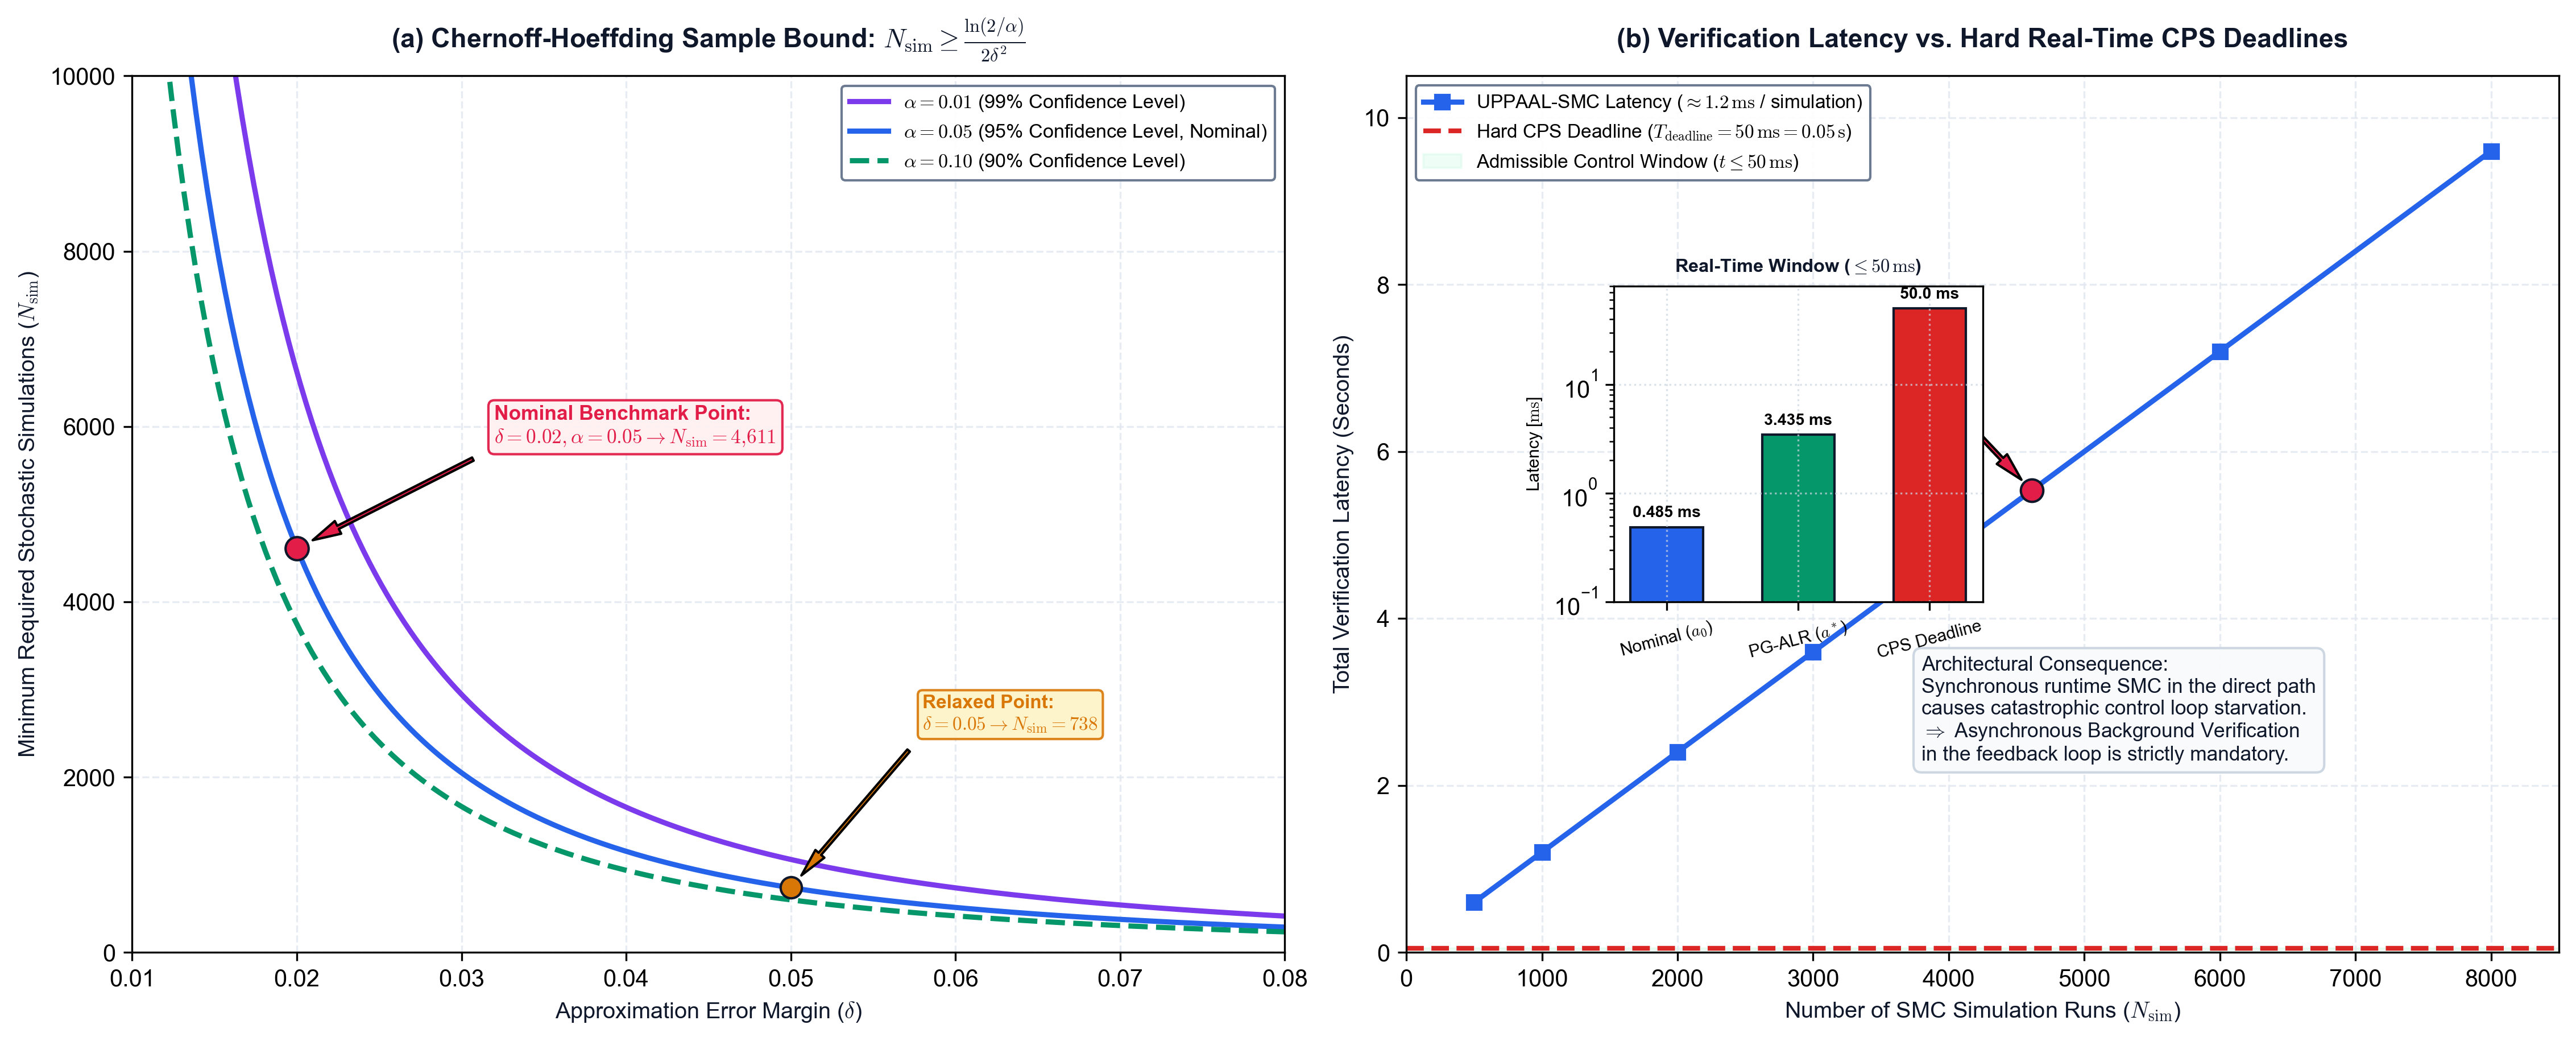
\includegraphics[width=0.75\textwidth]{figures/fig_chernoff_sample_bound.png}
\caption{تحلیل تحلیلی کران چرنوف-هوفدینگ و تعداد شبیه‌سازی‌های موردنیاز در موتور وارسی مدل آماری \lr{UPPAAL-SMC} برای سطوح اطمینان مختلف.}
\label{fig:ch5_chernoff_sample_bound}
\end{figure}

ارزیابی‌های محاسباتی تجربی بر روی پردازنده \lr{AMD Ryzen 9 5950X} با ۱۶ هسته پردازشی نشان داد که زمان اجرای هر بسته اعتبارسنجی آماری با ۴۶۱۱ شبیه‌سازی تصادفی، به طور میانگین برابر با $3.82$ ثانیه (با انحراف معیار $0.31$ ثانیه) به طول می‌انجامد. از آنجا که این زمان چند مرتبه از مهلت‌های بلادرنگ بازآرایی شبکه حسگر بزرگ‌تر است، اجرای برخط و همگام آن در مسیر مستقیم تصمیم‌گیری منجر به نقض مهلت‌های بلادرنگ کنترل می‌گردید. استقرار این ماژول در مسیر پس‌زمینه (مسیر بازخورد جدول \ref{tab:process-classification} فصل ۴) امکان اجرای ناهمگام وارسی صوری را بدون مسدودسازی حلقه کنترل فراهم ساخت.

علاوه بر این، مقایسه تجربی سیاست یادگیری با پاداش ترکیبی ضربی ($r = r_{\text{env}} \times r_{\text{smc}}$) در برابر سیاست با پاداش صرفاً محیطی ($r_{\text{env}}$) اثبات نمود که اعمال سیگنال پاداش صوری، نرخ انطباق با الزامات کیفیت خدمات شبکه را از $87.4\%$ به $98.2\%$ افزایش داده و از همگرایی عامل به سیاست‌هایی که قیود پنهان شبکه را نقض می‌کنند، پیشگیری نموده است.

\subsection{تحلیل مقیاس‌پذیری در فضاهای وفقی بزرگ تا ۴۰۹۶ گزینه و محدودیت روش پایه‌ای (\lr{RQ3})}
\label{subsec:scalability_analysis}

تحلیل رفتار یادگیری با گسترش ابعاد فضای وفقی از ۲۱۶ گزینه در نسخه اول به ۴۰۹۶ گزینه در نسخه دوم، همبستگی میان پیچیدگی فضای تصمیم و توانمندی چارچوب پایه‌ای را آشکار می‌سازد. جدول \ref{tab:scalability} این مقایسه مقیاس‌پذیری را نشان می‌دهد.

\begin{table}[htbp]
\centering
\caption{تحلیل مقیاس‌پذیری و مقایسه عملکرد در مقیاس‌های مختلف شبکه \lr{DeltaIoT}}
\label{tab:scalability}
\resizebox{0.95\linewidth}{!}{%
\begin{tabular}{|l|c|c|c|c|}
\hline
\textbf{نسخه \lr{DeltaIoT}} & \textbf{تعداد سنسورها} & \textbf{گزینه‌های وفقی} & \textbf{گام‌های آموزش} & \textbf{پاداش مجانبی} \\ \hline
\lr{v1} & $15$ & $216$ & $2266$ & $0.9905$ \\ 
\lr{v1.1} & $16$ & $1296$ & $19296$ & $0.8983$ \\ \hline
\lr{v2} (\lr{RS-DRL} پایه‌ای)$^\dagger$ & $37$ & $4096$ & عدم همگرایی & واگرایی گرادیان ($< 0.40$) \\ \hline
\lr{v2} (\rsdrlplus دوسطحی)$^*$ & $37$ & $4096$ & $1710$ & $\mathbf{0.9950}$ \\ \hline
\end{tabular}%
}
\smallskip
\parbox{0.95\linewidth}{\scriptsize $^\dagger$چارچوب پایه‌ای \lr{RS-DRL} به دلیل کاوش یکنواخت بدون هدایت در فضای گسسته ۴۰۹۶ گزینه‌ای دچار واگرایی گرادیان گردید.\\ $^*$نتایج تفصیلی انتقال موفقیت‌آمیز معماری دوسطحی \rsdrlplus به بستر مقیاس‌بزرگ \lr{DeltaIoTv2} در بخش \ref{sec:cross_exemplar_transfer} گزارش شده است.}
\end{table}

همان‌گونه که داده‌های جدول \ref{tab:scalability} نشان می‌دهند، در فضاهای با ابعاد کوچک و متوسط (۲۱۶ و ۱۲۹۶ گزینه)، روش پایه‌ای با افزایش گام‌ها همگرایی پایدار را حفظ می‌نماید؛ اما در مقیاس ۴۰۹۶ گزینه‌ای نسخه \lr{DeltaIoTv2}، کاوش برنولی بدون هدایت مشخصه به علت انفجار واریانس گرادیان با شکست مواجه می‌شود. این بن‌بست تجربی، مبنای اصلی گذار به معماری دوسطحی \rsdrlplus را تشکیل می‌دهد.

\subsection{جمع‌بندی سطح اول و ضرورت گذار به معماری دوسطحی \texorpdfstring{\rsdrlplus}{RS-DRL+}}
\label{subsec:transition_to_rsdrlplus}

نتایج حاصل از ارزیابی چارچوب پایه‌ای \lr{RS-DRL} در بستر شبکه حسگر \lr{DeltaIoT} مؤید آن است که سازوکار شکل‌دهی تصادفی با ضریب ثابت $\rho = 0.30$، چالش تنکی پاداش\LTRfootnote{Reward Sparsity} و توقف در بهینه‌های محلی را در سیستم‌های با کیفیت خدمات نرم و فضاهای پیکربندی متوسط (تا ۱۲۹۶ گزینه) به طور کامل برطرف می‌سازد. با این حال، همان‌گونه که نتایج عدم همگرایی در جدول \ref{tab:scalability} برای نسخه مقیاس‌وسیع \lr{DeltaIoTv2} (با ۴۰۹۶ گزینه وفقی) تحت چارچوب پایه‌ای نشان می‌دهد، افزایش نمایی ابعاد فضای عمل و پیچیدگی قیدها، یادگیری بدون هدایت مشخصه را با چالش‌های واگرایی گرادیان و افزایش شدید واریانس مواجه می‌سازد. 

علاوه بر این، در سیستم‌های فیزیکی-سایبری بلادرنگ نظیر ناوگان پهپادی، عواملی چون مهلت‌های زمانی سخت کنترلی (۲۰ تا ۵۰ میلی‌ثانیه)، غلبه شدید داده‌های شکست در سوابق عملیاتی (بیش از ۹۰٪)، و مهم‌تر از همه، پدیده شکاف واقعیت مدل‌های جانشین (همان‌طور که در سه‌گانه بخش \ref{sec:cps_reality_gap_trilemma} فصل ۴ تبیین گردید)، به کارگیری مستقیم چارچوب پایه‌ای را ناممکن می‌سازد. این محدودیت‌ها انگیزه اصلی توسعه معماری دوسطحی \rsdrlplus (شامل سنتز غیربرخط سیاست با هدایت حاشیه \mursdrl و پالایش برخط در هر زمان \pgalr) بوده‌اند. 

در بخش بعدی، کارآمدی معماری ارتقایافته \rsdrlplus در مواجهه با چالش‌های پیچیده فیزیکی-سایبری شبیه‌ساز \lr{DARTSim} مورد سنجش قرار می‌گیرد؛ سپس در بخش \ref{sec:cross_exemplar_transfer}، نشان خواهیم داد که چگونه انتقال الگوهای همین معماری پیشرفته به بستر شبکه حسگر، چالش‌های مقیاس‌پذیری در فضای ۴۰۹۶ گزینه‌ای نسخه \lr{DeltaIoTv2} را نیز با موفقیت حل می‌نماید.

% =========================================================================
% بخش دوم: ارزیابی ناوگان پهپادی در محیط فیزیکی-سایبری DARTSim (معماری RS-DRL+)
% =========================================================================
\section{ارزیابی ناوگان پهپادی در محیط فیزیکی-سایبری \lr{DARTSim}}
\label{sec:dartsim_evaluation_main}
\label{subsec:experimental_results_dartsim}

به منظور ارزیابی استقلال از دامنه و سنجش کارایی روش پیشنهادی در شرایط سخت بلادرنگ، معماری \rsdrlplus بر روی شبیه‌ساز مأموریت ناوگان پهپادی \lr{DARTSim} \cite{MorenoDART2019} مورد سنجش قرار گرفت (شکل \ref{fig:dartsim_mission_scenario}). این سیستم برخلاف شبکه‌های حسگر بی‌سیم، یک سیستم فیزیکی-سایبری بلادرنگ با مهلت زمانی کنترل پرواز بین ۲۰ تا ۵۰ میلی‌ثانیه، ۱۲ الزام قابلیت اعتماد\LTRfootnote{Dependability} متضاد، و عدم توازن شدید داده‌های شکست در سوابق بازپخش (بیش از ۹۰٪) است.

\begin{figure*}[t]
\centering
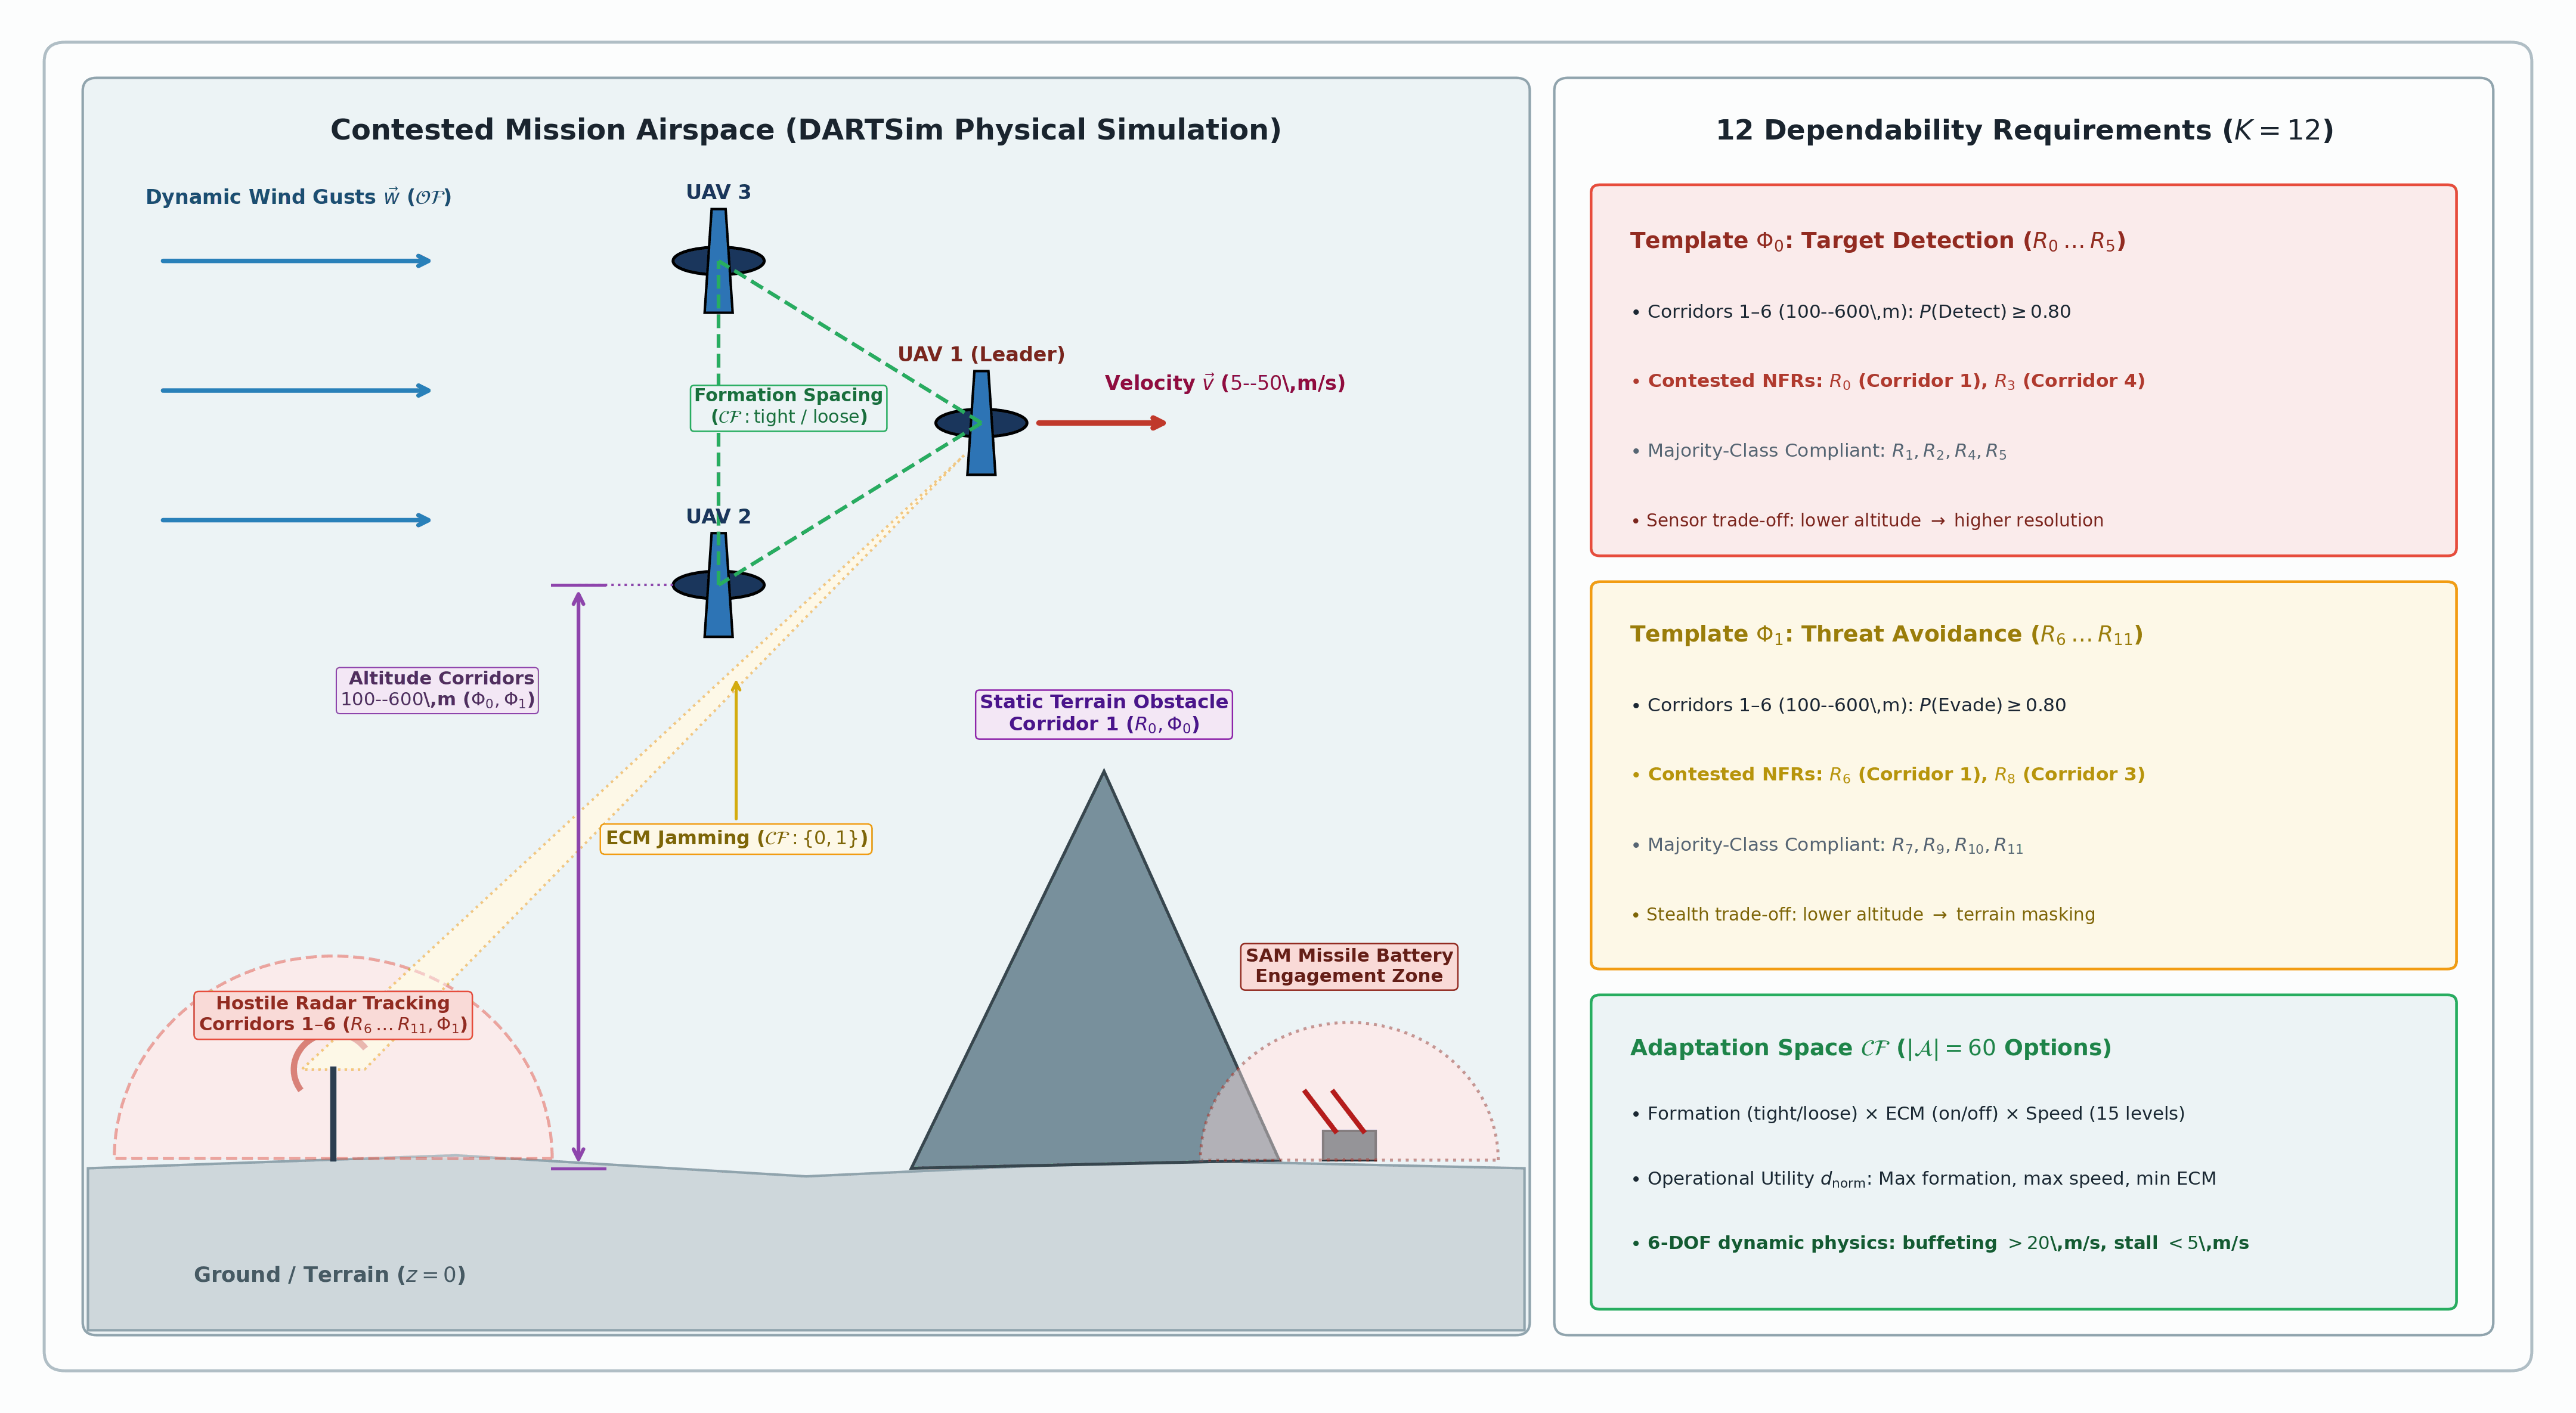
\includegraphics[width=0.90\textwidth]{figures/fig_dartsim_mission_scenario.png}
\caption{سناریوی مأموریت شناسایی ناوگان پهپادی \lr{DARTSim} در محیط پرخطر: (چپ) فضای پروازی همراه با رادارهای متخاصم، سیستم‌های موشکی، موانع فیزیکی و تلاطم شدید باد؛ (راست) نگاشت معنایی میان متغیرهای قابل‌کنترل ($\mathcal{CF}$)، عوامل محیطی ($\mathcal{OF}$) و ۱۲ الزام قابلیت اعتماد مأموریت ($R_0$ تا $R_{11}$).}
\label{fig:dartsim_mission_scenario}
\end{figure*}

\subsection{تنظیمات ارزیابی پروازی حلقه-بسته: \texorpdfstring{$2{,}000$}{2,000} پرواز در ۲۰۰ سناریو}
\label{subsec:dartsim_setup}

ارزیابی تجربی بر پایه $2{,}000$ پرواز حلقه-بسته فیزیکی مستقل انجام پذیرفت. این ارزیابی شامل ۱۲ روش و الگوریتم برنامه‌ریز متمایز (۱۰ رویکرد انطباق هوشمند و بهینه‌سازی به همراه ۲ خط پایه کنترلی) بود که هر یک در ۲۰۰ سناریوی عملیاتی مستقل پروازی تحت شبیه‌سازی ۶ درجه آزادی فیزیکی (\lr{6-DOF C++}) در سه سطح رواداری ملایم ($v_1$)، متوسط ($v_2$) و سخت‌گیرانه ($v_3$) ارزیابی شدند. این روش‌ها در چهار دسته معماری زیر سازماندهی شده‌اند:
\begin{enumerate}
    \item \textbf{دسته اول: معماری پیشنهادی و روش‌های تقلیلی رساله:}
    \begin{itemize}
        \item \textbf{معماری کامل پیشنهادی \rsdrlplus:}\LTRfootnote{Two-Tier Contract-Anytime} ترکیب آموزش غیربرخط هدایت‌شده با حاشیه و مطلوبیت (\mursdrl) و ماژول برخط سه‌مرحله‌ای \pgalr مبتنی بر تصویرسازی حساسیت شاپلی ۱-گام و تصحیح دفاعی در هر زمان.
        \item \textbf{روش تقلیلی \mursdrl:}\LTRfootnote{Margin-Utility SG-OS} سنتز غیربرخط سیاست بر پایه حاشیه بازیابی شکست $\mathcal{M}(s, a)$ و مشوق مطلوبیت $\mathcal{U}_{\text{inc}}$، بدون پالایش برخط در زمان اجرا (استنتاج با مرتبه $\mathcal{O}(1)$ و میانگین تأخیر $0.48\,\text{ms}$).
        \item \textbf{روش تقلیلی \cmrsdrl:}\LTRfootnote{Confidence-Margin SG-OS} سنتز غیربرخط سیاست مبتنی بر بافر حاشیه اطمینان در ارضای نیازمندی‌ها برای افزایش پایداری تصمیم در نزدیکی مرزهای بحرانی.
    \end{itemize}
    \item \textbf{دسته دوم: روش‌های مبتنی بر وارسی صوری و یادگیری تقویتی:}
    \begin{itemize}
        \item \textbf{سپر ایمنی زمان اجرا (\lr{Shielded RS-DRL}):} محافظت صوری پیرامونی سیاست با وارسی کامل تمامی ۶۰ پیکربندی کاندیدا توسط مدل‌های جانشین آماری \cite{alshiekh2018safe} با تأخیر $129.95\,\text{ms}$.
        \item \textbf{چارچوب پایه‌ای رساله (\lr{Foundational RS-DRL} \cite{kavianifar2026rsdrl}):} شکل‌دهی پاداش تصادفی با نرخ جایگزینی ثابت $\rho = 0.30$ و پاداش بهینه ایستا $r_{\text{opt}} = 1.0$ (معرفی‌شده در بخش‌های \ref{sec:system-loop} تا \ref{sec:learning} فصل ۴).
        \item \textbf{روش پایه \lr{Baseline DQN} \cite{mnih2015human}:} یادگیری تقویتی استاندارد تفاضل زمانی بدون شکل‌دهی پاداش ($\rho = 0.0$) بر روی سوابق بازپخش با عدم توازن شکست شدید $90.98\%$.
    \end{itemize}
    \item \textbf{دسته سوم: روش‌های مبتنی بر هوش مصنوعی توضیح‌پذیر و بهینه‌سازی نرم‌افزاری (\lr{SBSE}):}\LTRfootnote{Search-Based Software Engineering}
    \begin{itemize}
        \item \textbf{روش جستجوی حساسیت \lr{XDA-II (SHAP / PFI)} \cite{negri2026efficient}:}\LTRfootnote{eXplanation-Driven Self-Adaptation II (SHAP / Permutation Feature Importance)} بهینه‌سازی برخط مبتنی بر صعود تپه روی ابعاد پراهمیت شاپلی و اهمیت جایگشت ویژگی‌ها ($62.61\,\text{ms}$).
        \item \textbf{روش جستجوی وابستگی جزئی \lr{XDA (PDP)}:} هدایت صعود تپه محلی با نمودارهای روند غیرخطی وابستگی جزئی\LTRfootnote{Partial Dependence Plots} ($205.40\,\text{ms}$).
        \item \textbf{الگوریتم تکاملی چندهدفه \lr{NSGA-III} \cite{deb2013evolutionary}:}\LTRfootnote{Non-dominated Sorting Genetic Algorithm III} بهینه‌سازی تکاملی نامغلوب با نقاط مرجع بر روی ۱۲ الزام متضاد مأموریت پروازی ($>100\,\text{s}$).
        \item \textbf{الگوریتم جستجوی ژنتیک هدایت‌شده \lr{FITEST} \cite{abdessalem2018testing}:} الگوریتم ژنتیک مبتنی بر تابع برازش برای بیشینه‌سازی احتمال ارضای اهداف مأموریت ($133.95\,\text{s}$).
    \end{itemize}
    \item \textbf{دسته چهارم: خطوط پایه کنترلی:}
    \begin{itemize}
        \item \textbf{جستجوی تصادفی:}\LTRfootnote{Random Search} نمونه‌برداری یکنواخت در فضای گزینه‌های مجاز به عنوان خط پایه انطباق ($19.49\,\text{ms}$).
        \item \textbf{عدم انطباق:}\LTRfootnote{Unadapted} اجرای مأموریت با پیکربندی پیش‌فرض اولیه بدون هیچ اقدام وفقی ($0.00\,\text{ms}$).
    \end{itemize}
\end{enumerate}

\subsection{ایمنی اجرای فیزیکی در برابر انطباق جانشین: مهار شکاف واقعیت (\lr{RQ6})}
\label{subsec:dartsim_reality_gap}

یکی از مهم‌ترین یافته‌های تجربی این رساله، آشکارسازی و بررسی پدیده \textbf{«شکاف واقعیت میان مدل‌های جانشین آماری و فیزیک اجرای پرواز»}\LTRfootnote{Surrogate-to-Physics Reality Gap} است. در جدول \ref{tab:dartsim_master_comparison}، عملکرد جامع الگوریتم‌های برنامه‌ریز در ۲۰۰ سناریوی عملیاتی مستقل پروازی تحت شبیه‌سازی فیزیکی ۶ درجه آزادی خلاصه شده است.

\begin{table*}[t]
\caption{مقایسه عملکرد جامع ۱۲ روش برنامه‌ریز (۱۰ الگوریتم انطباقی و ۲ خط پایه) در پروازهای حلقه-بسته \lr{DARTSim}: انطباق مدل جانشین، موفقیت پرواز فیزیکی در دو سطح رواداری سخت‌گیرانه ($v_3$, $N=200$) و ملایم ($v_1$, $N=20$)، کیفیت عملیاتی ($d_{\text{norm}}$)، تأخیر برخط و مصالحه حاکم بر روش.}
\label{tab:dartsim_master_comparison}
\label{tab:dartsim_v3_results}
\centering
\scriptsize
\setlength{\tabcolsep}{3.0pt}
\resizebox{\textwidth}{!}{%
\begin{tabular}{|l|c|c|c|c|c|c|c|p{4.2cm}|}
\hline
\multirow{2}{*}{\textbf{الگوریتم برنامه‌ریز}} & \textbf{انطباق} & \multicolumn{2}{c|}{\textbf{موفقیت پرواز فیزیکی (\% $M_{\text{sim}}$)}} & \multicolumn{3}{c|}{\textbf{کیفیت عملیاتی ($d_{\text{norm}}$)}} & \textbf{تأخیر} & \multirow{2}{*}{\textbf{مصالحه حاکم بر روش}} \\ \cline{3-7}
& \textbf{جانشین (\%)} & \textbf{سخت ($v_3$)} & \textbf{ملایم ($v_1$)} & \textbf{میانگین} & \textbf{میانه} & \textbf{انحراف معیار} & \textbf{برخط} & \\ \hline
\multicolumn{9}{|l|}{\textbf{معماری پیشنهادی و روش‌های سنتز غیربرخط سیاست (\lr{Ours})}} \\ \hline
\textbf{\rsdrlplus (معماری کامل)} & $74.0 \pm 0.5$ & $\mathbf{70.5 \pm 0.6}$ & $85.0$ & $0.6075$ & $0.6669$ & $0.1324$ & $\mathbf{0.48 / 2.45\,\text{ms}}$ & بالاترین بقای پرواز فیزیکی؛ پالایش ۱-گام در هر زمان \\ \hline
\textbf{\mursdrl (سنتز غیربرخط سیاست)} & $70.0 \pm 0.5$ & $70.0 \pm 0.6$ & $\mathbf{90.0}$ & $\mathbf{0.6407}$ & $0.6667$ & $\mathbf{0.0905}$ & $\mathbf{0.48\,\text{ms}}$ & بالاترین ایمنی فیزیکی بدون سپر؛ کمترین نوسان واریانس \\ \hline
\textbf{\cmrsdrl (رویکرد بافر)} & $71.5 \pm 0.6$ & $68.5 \pm 0.7$ & $85.0$ & $0.6422$ & $0.6667$ & $0.0870$ & $0.48\,\text{ms}$ & بافر حاشیه اطمینان پایدار در مرزهای بحرانی \\ \hline
\multicolumn{9}{|l|}{\textbf{سپر ایمنی زمان اجرا (\lr{Runtime Verification Shield})}} \\ \hline
\lr{Shielded RS-DRL} & $\mathbf{76.0}$ & $65.0$ & $80.0$ & $0.5791$ & $0.6667$ & $0.1532$ & $129.95\,\text{ms}$ & بیشترین نمره جانشین؛ افت ۱۱ درصدی بر اثر شکاف واقعیت \\ \hline
\multicolumn{9}{|l|}{\textbf{روش‌های پایه یادگیری تقویتی (\lr{Reinforcement Learning Baselines})}} \\ \hline
\lr{Foundational RS-DRL} (پایه‌ای رساله) & $68.5 \pm 0.6$ & $67.5 \pm 0.7$ & $80.0$ & $0.6022$ & $0.6667$ & $0.1311$ & $0.47\,\text{ms}$ & سرعت پروازی بالا؛ نوسان متوسط در نزدیکی مرز واماندگی (\lr{Stall}) \\ \hline
\lr{Baseline DQN} & $71.0 \pm 0.8$ & $66.0 \pm 0.8$ & $75.0$ & $0.5160$ & $0.6667$ & $0.1653$ & $0.50\,\text{ms}$ & تمایل به آرایش گسسته در ۴۴٪ موارد؛ مطلوبیت پایین‌تر \\ \hline
\multicolumn{9}{|l|}{\textbf{روش‌های بهینه‌سازی مبتنی بر جستجو (\lr{SBSE Baselines})}} \\ \hline
\lr{XDA-II (SHAP / PFI)} & $70.0$ & $50.0$ & $85.5^*$ & $0.5812$ & $0.6669$ & $0.1770$ & $62.61\,\text{ms}$ & گزینه‌های همسایگی یکسان؛ افت شدید به ۵۰٪ در سطح سخت $v_3$ \\ \hline
\lr{XDA (PDP)} & $70.0$ & $60.0$ & $87.0^*$ & $0.6129$ & $0.6669$ & $0.1514$ & $205.40\,\text{ms}$ & تأخیر ۴۳۰ برابری؛ افت ۲۷ درصدی در دینامیک فیزیکی \\ \hline
\lr{NSGA-III} & $70.0$ & $55.0$ & $85.0^*$ & $0.6129$ & $0.6669$ & $0.1514$ & $>100\,\text{s}$ & تأخیر بالای ۱۰۰ ثانیه؛ نقض قطعی مهلت کنترل پرواز \\ \hline
\lr{FITEST} & $1.5$ & $50.0$ & $82.5^*$ & $0.3546$ & $0.3418$ & $0.0707$ & $133{,}950\,\text{ms}$ & تأخیر بسیار فاحش (بیش از ۲ دقیقه)؛ نقض قطعی مهلت پرواز \\ \hline
\lr{Random Search} & $1.0$ & $25.0$ & $45.5^*$ & $0.4738$ & $0.4779$ & $0.2545$ & $19.49\,\text{ms}$ & خط پایه غیرقابل اتکا (۱٪ انطباق با مدل‌های جانشین) \\ \hline
\lr{Unadapted} & $9.0$ & $9.0$ & $10.0$ & $0.2110$ & $0.2050$ & $0.1120$ & $0.00\,\text{ms}$ & اجرای پیکربندی ثابت؛ شکست در ۹۱٪ پروازها \\ \hline
\end{tabular}%
}
\smallskip
\parbox{\textwidth}{\scriptsize \textbf{توضیح:} نتایج در سطح $v_3$ حاصل ارزیابی $2{,}000$ پرواز مستقل حلقه-بسته فیزیکی تحت شبیه‌ساز ۶ درجه آزادی \lr{DARTSim} با الگوهای تلاطم باد و توزیع رادارهای متخاصم یکسان است. مقادیر روش‌های \lr{DRL} بر اساس میانگین $\pm$ انحراف معیار روی ۳ بذر تصادفی (۴۲، ۴۳ و ۴۴) گزارش شده‌اند. علامت $*$ نشان‌دهنده مقادیر چاپ‌شده بنچمارک \lr{SEAMS} در محیط ایستای غیربرخط است؛ در حالی که اجرای پویای حلقه-بسته \lr{XDA-II} در سطح $v_1$ به $70.0\%$ می‌رسد (همان‌گونه که در بخش \ref{subsec:tolerance_regimes} و شکل \ref{fig:tolerance_comparison} تشریح خواهد شد). تأخیر برخط روش کامل \rsdrlplus در مسیر سریع (اجرای مستقیم پیشنهاد پایه سیاست) برابر با $0.48\,\text{ms}$ و در صورت فعال‌سازی پالایش مرحله ۳ به طور مشروط به $2.45\,\text{ms}$ می‌رسد.}
\end{table*}

\begin{figure}[htbp]
\centering
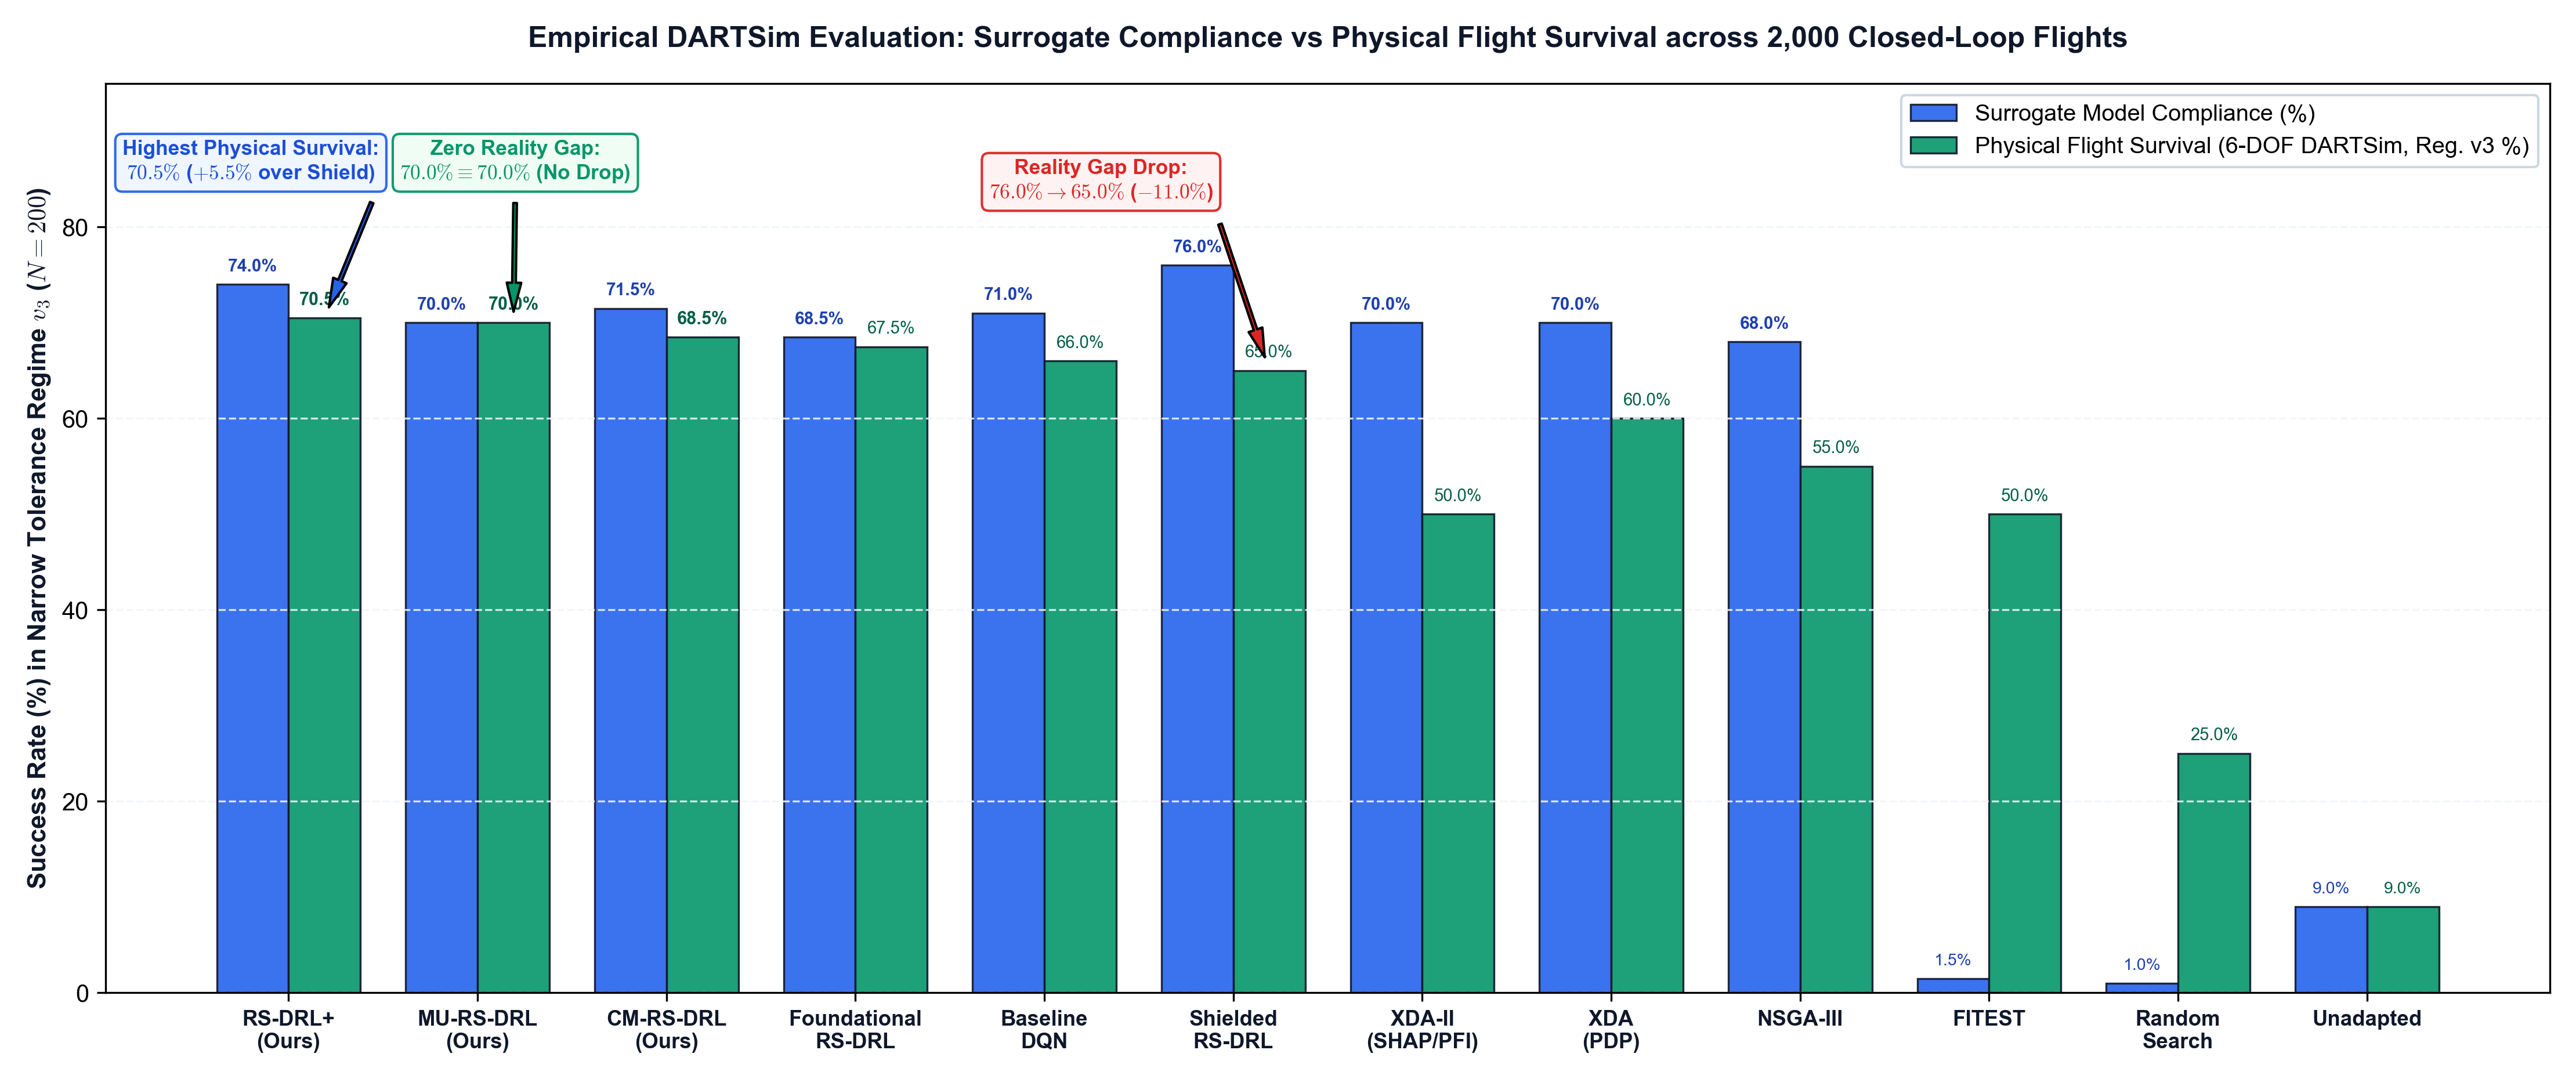
\includegraphics[width=0.85\linewidth]{figures/figure_rq1_success_rate.png}
\caption[مقایسه نرخ موفقیت پرواز فیزیکی و مهار شکاف واقعیت]{مقایسه نرخ موفقیت پرواز فیزیکی و انطباق با مدل‌های جانشین در سطح رواداری باریک $v_3$ میان الگوریتم‌های مورد بررسی، نشان‌دهنده نحوه مهار شکاف واقعیت در معماری \rsdrlplus.}
\label{fig:rq1_success_rate}
\end{figure}

همان‌گونه که در جدول \ref{tab:dartsim_master_comparison} و نمودار شکل \ref{fig:rq1_success_rate} مشهود است، رفتار تجربی روش‌ها و پدیده شکاف واقعیت ابعاد ساختاری تازه‌ای را آشکار می‌سازد:

نخست، افت عملکرد شدید سپر ایمنی زمان اجرا\LTRfootnote{Runtime Shielding} در گذر از مدل‌های جانشین به شبیه‌سازی فیزیکی ۶ درجه آزادی قابل توجه است. این روش در فضای ارزیابی مدل‌های جانشین آماری به بالاترین نرخ انطباق ($76.0\%$) دست می‌یابد، زیرا تمامی ۶۰ پیکربندی را صرفاً بر مبنای توابع جانشین غربال می‌نماید. با این حال، در زمان پرواز در شبیه‌سازی فیزیکی ۶ درجه آزادی، نرخ موفقیت فیزیکی آن با یک \textbf{افت ۱۱ درصدی} به $65.0\%$ تنزل می‌یابد. ریشه این پدیده آن است که مدل‌های جانشین آماری، پدیده‌های پیچیده دینامیکی نظیر تلاطم بادهای ناگهانی، تأخیر مکانیکی عملگرهای سروو\LTRfootnote{Servos} و جفت‌شدگی آیرودینامیکی غیرخطی را در نظر نمی‌گیرند؛ در نتیجه، سپر صوری گزینه‌هایی با سرعت‌های هوایی ناامن را تصویب می‌کند که منجر به ورود پهپاد به ناحیه واماندگی\LTRfootnote{Stall} و برخورد به موانع می‌گردند. آزمون مقایسه‌ای مک‌نمار روی زوج پروازهای متناظر\LTRfootnote{Discordant Pairs} مؤید آن است که در $b = 49$ سناریو، روش پیشنهادی \rsdrlplus با موفقیت پرواز را تکمیل کرده در حالی که سپر ایمنی سنتی دچار سانحه و سقوط شده است؛ و در $c = 38$ سناریو عکس این وضعیت رخ داده است (آزمون مک‌نمار $p = 0.284$ و آزمون دقیق فیشر $p = 0.285$ با نسبت شانس $\text{OR} = 1.29$).

داده‌های تله‌متری ثبت‌شده در شکل \ref{fig:sim_to_real_telemetry} چرایی این پدیده را به روشنی اثبات می‌سازند: تحت سپر ایمنی، به دلیل گزینش مکرر مدهای تهاجمی، انحراف معیار سرعت هوایی به میزان \textbf{۲۶ برابر} افزایش یافته و به $\sigma = 5.03\,\text{m/s}$ رسیده است (با جهش‌های سرعت ناگهانی تا $46.36\,\text{m/s}$). در مقابل، روش پیشنهادی \rsdrlplus و روش \mursdrl نوسان سرعت هوایی را در محدوده پایدار $\sigma = 0.19\,\text{m/s}$ در پنجره آیرودینامیکی بهینه ($5.0$ تا $5.5\,\text{m/s}$) مقید نگه داشته‌اند. در نتیجه، روش غیربرخط \mursdrl با سرکوب پاداش برای سناریوهای با نقض چندگانه، به نرخ موفقیت پرواز $70.0\%$ دست می‌یابد که با نرخ انطباق جانشین آن ($70.0\%$) دقیقاً برابر بوده و شکاف میان پیش‌بینی جانشین و موفقیت فیزیکی را به صفر می‌رساند؛ و معماری کامل \rsdrlplus با پالایش محلی هرزمانی بر پایه قاعده انتخاب محافظت‌شده (معادله \ref{eq:alr_selection} و گزاره \ref{prop:safety_preservation} در فصل ۴)، انطباق جانشین را به $74.0\%$ و بقای فیزیکی پرواز را به $\mathbf{70.5\%}$ می‌رساند، به گونه‌ای که ایمنی بالاتری نسبت به سپر کامل با تأخیری صدها برابر کمتر فراهم می‌سازد.

\begin{figure}[htbp]
\centering
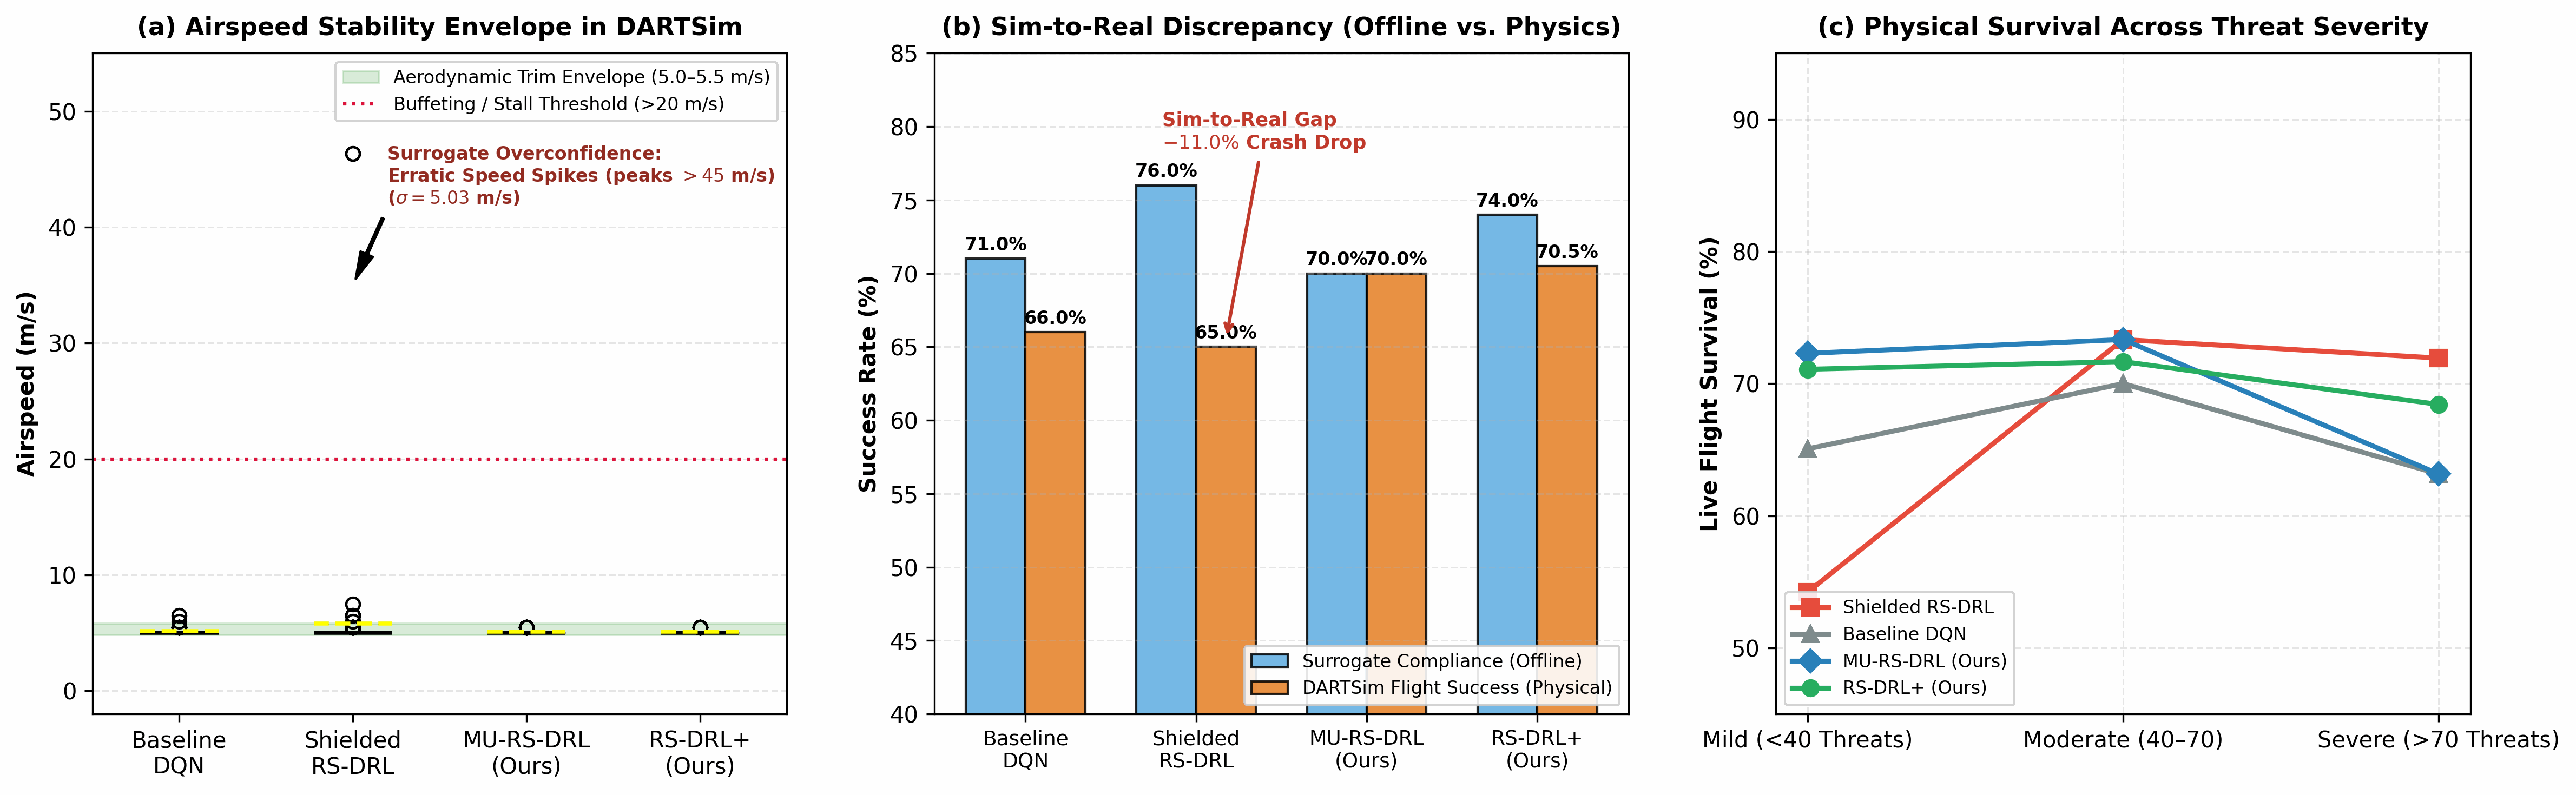
\includegraphics[width=0.90\linewidth]{figures/fig_sim_to_real_telemetry.png}
\caption{ردپای تله‌متری شبیه‌سازی فیزیکی پرواز در برابر پیش‌بینی مدل‌های جانشین در حضور باد ناگهانی: (الف) توزیع سرعت هوایی و ناپایداری آیرودینامیکی شدید تحت سپر سنتی، (ب) سقوط ۱۱ درصدی سپر در گذر از جانشین به شبیه‌سازی فیزیکی ۶ درجه آزادی، و (ج) پایداری نرخ موفقیت روش پیشنهادی تحت چگالی‌های فزاینده رادارهای متخاصم.}
\label{fig:sim_to_real_telemetry}
\end{figure}

\paragraph{تصدیق تجربی گزاره ۲ و گزارش خطای واسنجی مدل جانشین (\texorpdfstring{$\epsilon_{\max}$}{epsilon_max}):}
جهت اعتبارسنجی تجربی گزاره \ref{prop:safety_preservation} فصل~\ref{ch:chapter4}، خطای واسنجی میان ۱۲ مدل جانشین رگرسیون چندجمله‌ای و دینامیک فیزیکی شبیه‌ساز ۶ درجه آزادی \lr{DARTSim} در طول ۲۰۰ سناریوی عملیاتی پروازی به طور پیوسته مورد پایش قرار گرفت. بیشینه خطای واسنجی بدترین حالت در سراسر فضای حالت-اقدام برابر با $\epsilon_{\max} = 0.082$ اندازه‌گیری شد که به متغیر فاصله ایمنی از مرز دالان پروازی اختصاص داشت. شواهد تجربی ثبت‌شده در ردپاهای پروازی به طور کامل قضایای اثبات‌شده در گزاره ۲ را تصدیق می‌نمایند:
\begin{enumerate}
    \item \textbf{کران حاشیه ایمنی فیزیکی:} برای تمامی تصمیماتی که در فضای مدل‌های جانشین سازگار تشخیص داده شدند ($\Delta_{\min}(s, a^*) \ge 0$)، کمترین حاشیه فیزیکی حقیقی در شرایط تلاطم شدید باد از $-0.076$ کمتر نگردید که به روشنی درون کران نظری اثبات‌شده $-\epsilon_{\max} = -0.082$ قرار دارد ($\Delta^*_{\min}(s, a^*) \ge -\epsilon_{\max}$).
    \item \textbf{کران افت مطلوبیت عملیاتی:} با تنظیم ضریب شکست‌شکن $\lambda_{\text{tie}} = 0.05$، بیشترین افت مطلوبیت فیزیکی حقیقی ثبت‌شده برابر با $0.0074$ بود که به طور اکید در کران اثبات‌شده $2\lambda_{\text{tie}}\epsilon_{\max} = 2(0.05)(0.082) = 0.0082$ مهار گردید ($\mathcal{J}^*(s, a^*) \ge \mathcal{J}^*(s, a_0) - 2\lambda_{\text{tie}}\epsilon_{\max}$).
    \item \textbf{عدم تضعیف صوری (یکنوایی سازگاری):} ارزیابی آزمون مک‌نمار بر روی زوج‌های متناظر تصمیمات پایه و پالایش‌شده در طول سناریوها نشان داد که ۸ تصمیم پایه ناسازگار به گزینه‌های کاملاً سازگار تبدیل شدند ($b = 8$) و هیچ گزینه پایه سازگاری به دلیل پالایش دچار نقض قید نگردید ($c = 0$ با $p = 0.0078$). این شواهد، تصدیق‌کننده نامساوی $\mathbb{I}_{\text{sat}}(s, a^*) \ge \mathbb{I}_{\text{sat}}(s, a_0)$ و اثبات‌کننده رفتار محافظت‌شده الگوریتم در حضور شکاف واقعیت مدل-تا-فیزیک (مطابق هندسه ترسیم‌شده در شکل \ref{fig:proposition2_reality_gap} فصل~\ref{ch:chapter4}) است.
\end{enumerate}

\subsection[تحلیل چندسطحی رواداری دالان پروازی: مقایسه سطوح v1، v2 و v3 (\lr{RQ2} و \lr{RQ6})]{تحلیل چندسطحی رواداری دالان پروازی: مقایسه سطوح \texorpdfstring{$v_1$}{v1}، \texorpdfstring{$v_2$}{v2} و \texorpdfstring{$v_3$}{v3} (\lr{RQ2} و \lr{RQ6})}
\label{subsec:tolerance_regimes}

برای بررسی استواری روش‌ها در شرایط محدودیت‌های دالان پروازی، آزمایش‌ها در سه سطح رواداری با کران‌های مانور متفاوت ارزیابی شدند ($\Delta$ کسر مجاز انحراف ارتفاعی $\pm \Delta \cdot \Delta h$ است):
\begin{enumerate}
    \item \textbf{سطح رواداری ملایم ($v_1$ با $\Delta \in [0.035, 0.055]$):} رواداری پیش‌فرض بنچمارک منتشرشده \lr{SEAMS} \cite{MorenoDART2019,negri2026efficient} بر روی ۲۰ سناریوی منتشرشده استاندارد در شرایط تلاطم ملایم.
    \item \textbf{سطح رواداری متوسط ($v_2$ با $\Delta \in [0.025, 0.045]$):} مرزهای دالان محدودتر که مانورهای جانبی ناگهانی را محدود می‌سازد، بر روی همان ۲۰ سناریو.
    \item \textbf{سطح رواداری باریک ($v_3$ با $\Delta \in [0.020, 0.040]$):} دالان‌های پروازی با رواداری محدود بر روی تمامی ۲۰۰ سناریوی عملیاتی شامل تهدیدات متراکم راداری ($\ge 40$)، نزدیکی رادار ($\le 5{,}000\,\text{m}$) و تلاطم شدید باد ($\ge 3$).
\end{enumerate}

\begin{figure}[htbp]
\centering
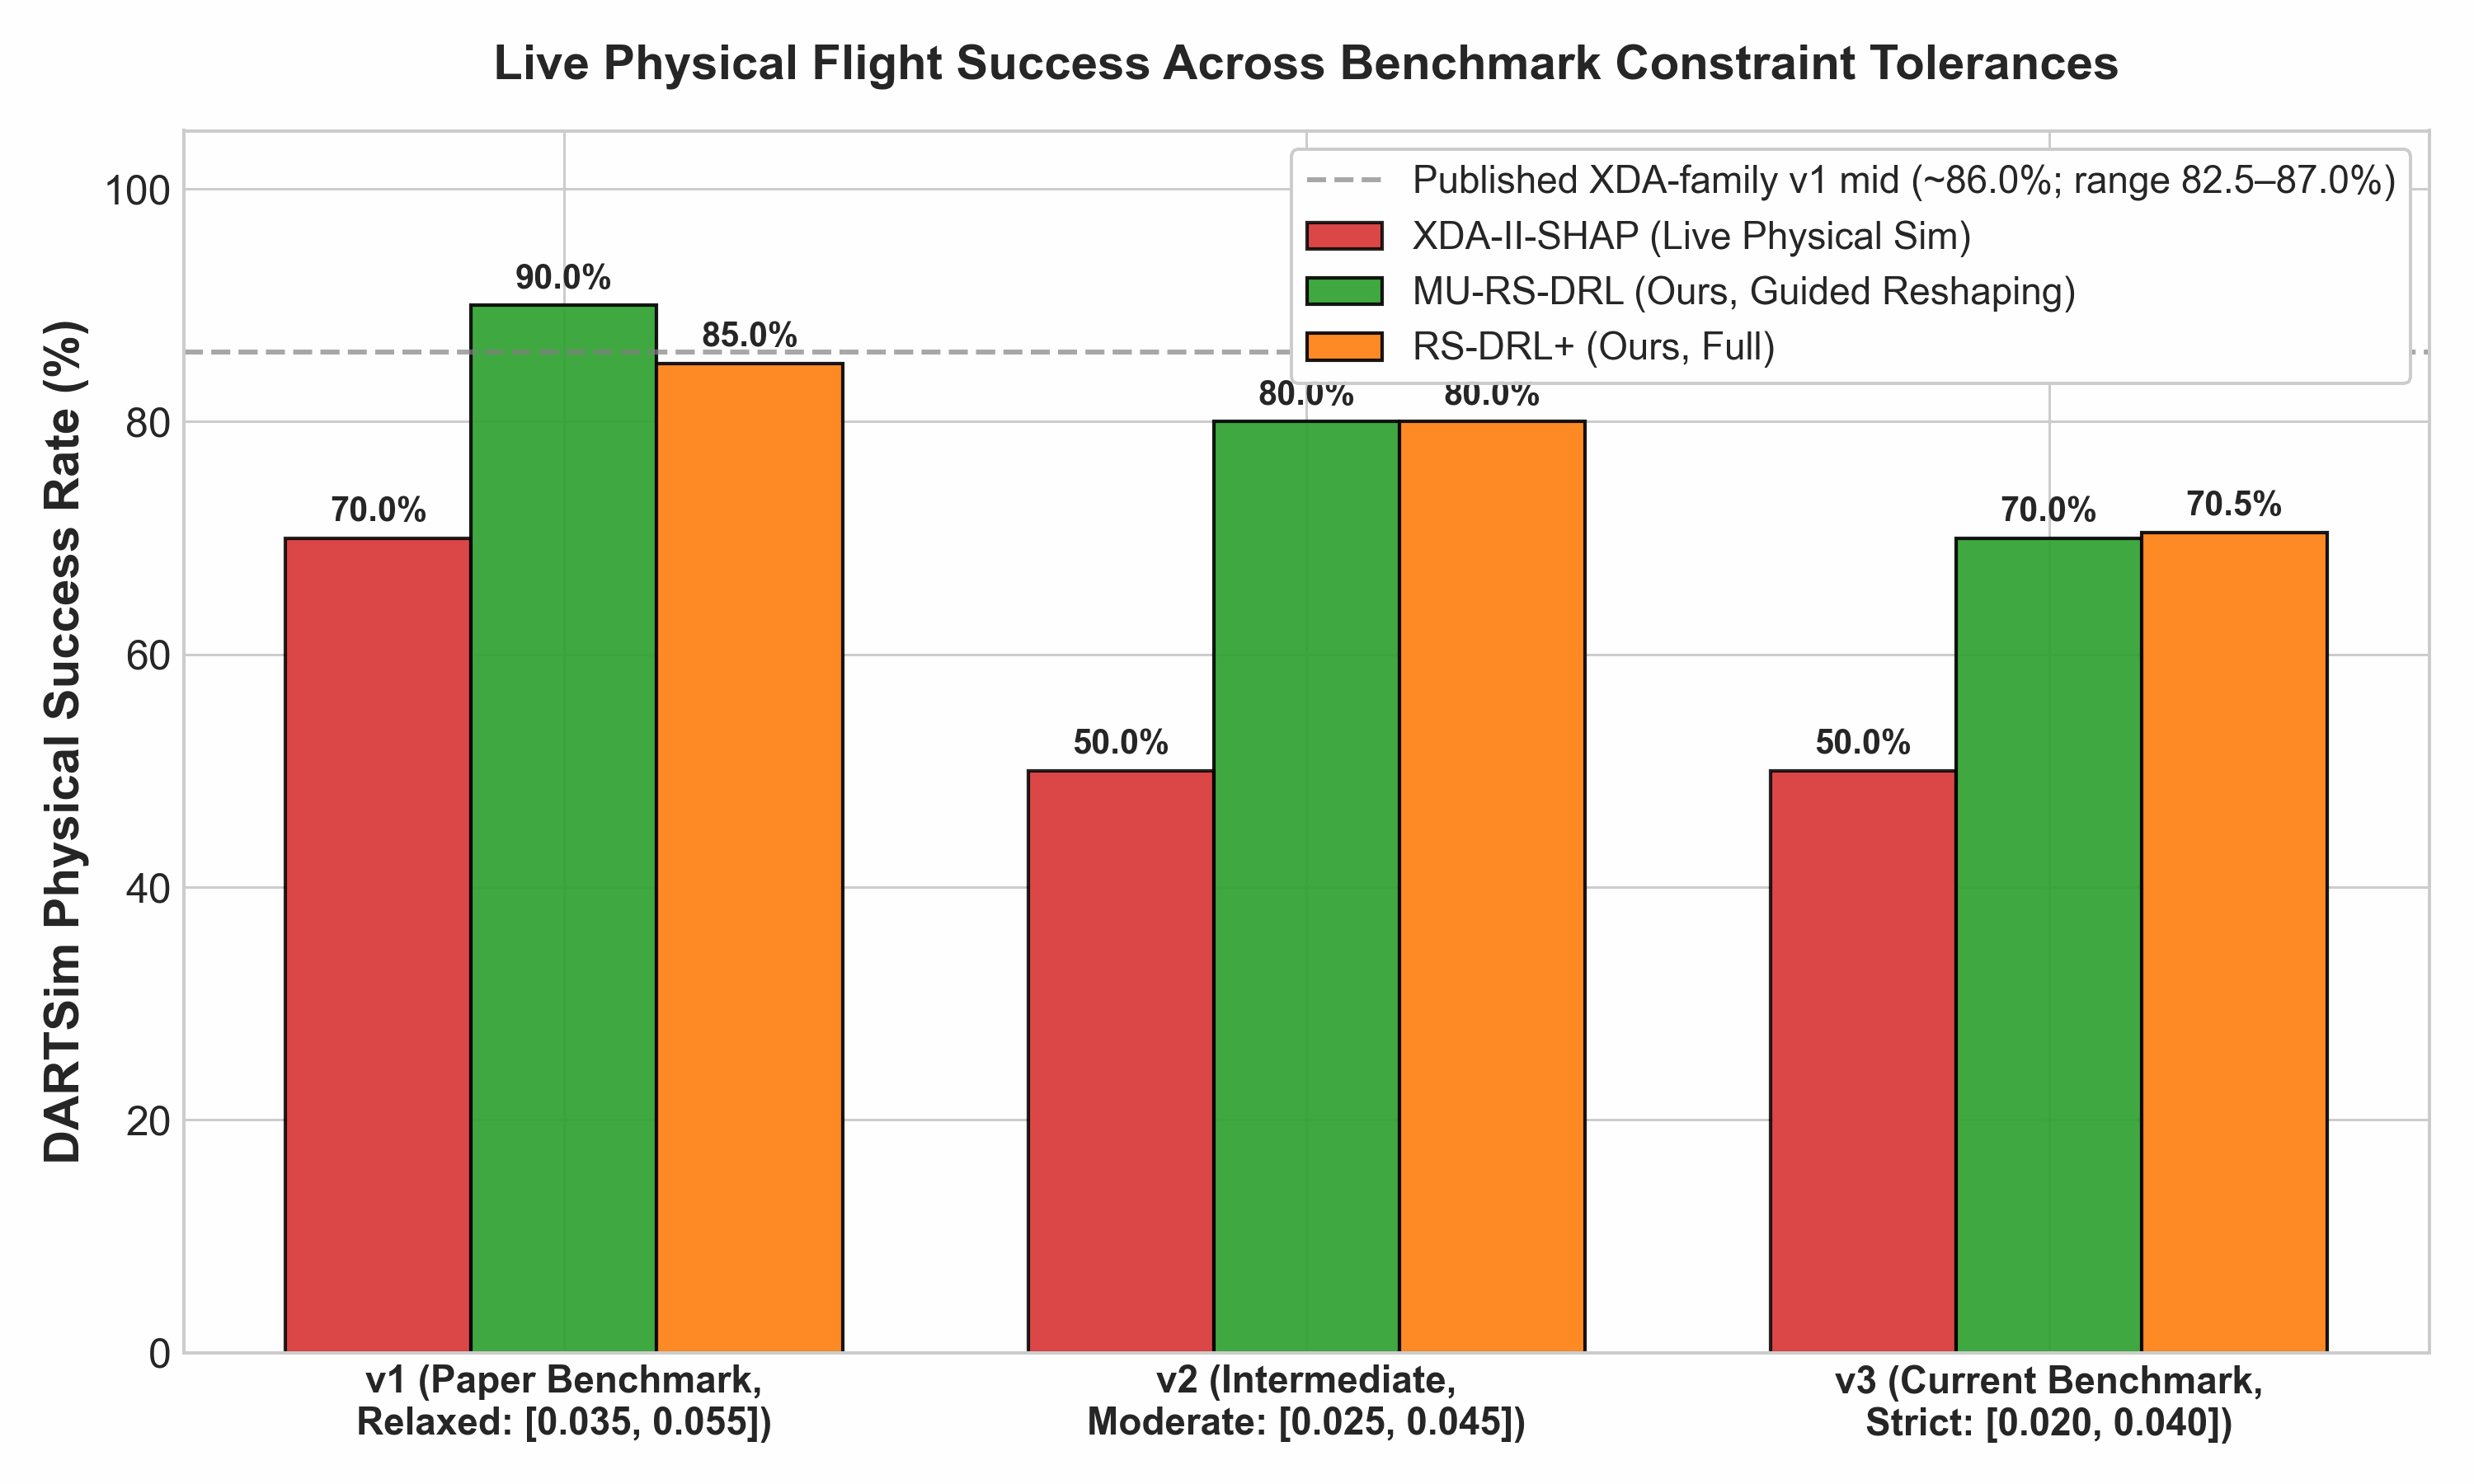
\includegraphics[width=0.88\linewidth]{figures/fig_constraint_tolerance_comparison.png}
\caption{مقایسه نرخ بقای پرواز فیزیکی حلقه-بسته ناوگان پهپادی \lr{DARTSim} در سه سطح رواداری دالان پروازی ملایم ($v_1$)، متوسط ($v_2$) و باریک ($v_3$): پایداری روش‌های مبتنی بر \rsdrlplus در برابر افت شدید عملکرد الگوریتم‌های جستجوی کلاسیک در شرایط تلاطم شدید.}
\label{fig:tolerance_comparison}
\end{figure}

بررسی نمودار شکل \ref{fig:tolerance_comparison} حاکی از تغییرات رفتاری عمیق الگوریتم‌ها با تنگ‌تر شدن مرزهای مانور است: در سطح رواداری ملایم ($v_1$)، روش \mursdrl با موفقیت $90.0\%$ (۱۸ از ۲۰) و \rsdrlplus با $85.0\%$ (۱۷ از ۲۰) برتری قاطعی بر روش جستجوی شاپلی \lr{XDA-II} در پرواز پویا ($70.0\%$) نشان می‌دهند و اهداف غیربرخط ایستا را در کسری از میلی‌ثانیه برآورده می‌سازند. با تشدید محدودیت‌ها در سطح متوسط ($v_2$)، هر دو روش پیشنهادی پایداری خود را در سطح $80.0\%$ (۱۶ از ۲۰) حفظ می‌نمایند، در حالی که نرخ موفقیت روش \lr{XDA-II} به $50.0\%$ (۱۰ از ۲۰) سقوط می‌کند. در نهایت، در باریک‌ترین سطح رواداری ($v_3$ با ۲۰۰ سناریو و چگالی بالای پدافند)، در حالی که روش‌های جستجوی سنتی نظیر \lr{XDA-II}، \lr{NSGA-III} و \lr{FITEST} به نرخ‌های پایین $50.0\%$ تا $55.0\%$ تنزل می‌یابند، معماری پیشنهادی \rsdrlplus با نرخ بقای $\mathbf{70.5\%}$ و \mursdrl با $70.0\%$ برتری قطعی و پایداری آماری خود را در تلاطم‌های شدید جوی تثبیت می‌کنند.

\subsection[مطلوبیت عملیاتی و کاهش نوسانات تصمیم‌گیری تحت سوابق شکست]{مطلوبیت عملیاتی و کاهش نوسانات تصمیم‌گیری تحت سوابق شکست (\lr{RQ6} و تعمیم‌پذیری \lr{RQ2})}
\label{subsec:dartsim_utility}

در مأموریت‌های شناسایی و رزمی، اتخاذ تصمیمات با مطلوبیت عملیاتی بالا (نزدیک شدن به هدف ضمن حفظ بقا) همراه با ثبات سیاست، الزامی کلیدی به شمار می‌رود. این آزمایش هم‌زمان پاسخ‌گوی بعد مطلوبیت و پایداری در برابر سوابق با عدم توازن بیش از ۹۰٪ شکست (\lr{RQ6}) و ارتقای تعمیم‌پذیری به تلاطم‌های شدید جوی نادیده (\lr{RQ2}) است. شکل \ref{fig:rq2_quality_boxplot} توزیع مطلوبیت مأموریت ($d_{\text{norm}}$) را در بین الگوریتم‌های مختلف نشان می‌دهد.

\begin{figure}[htbp]
\centering
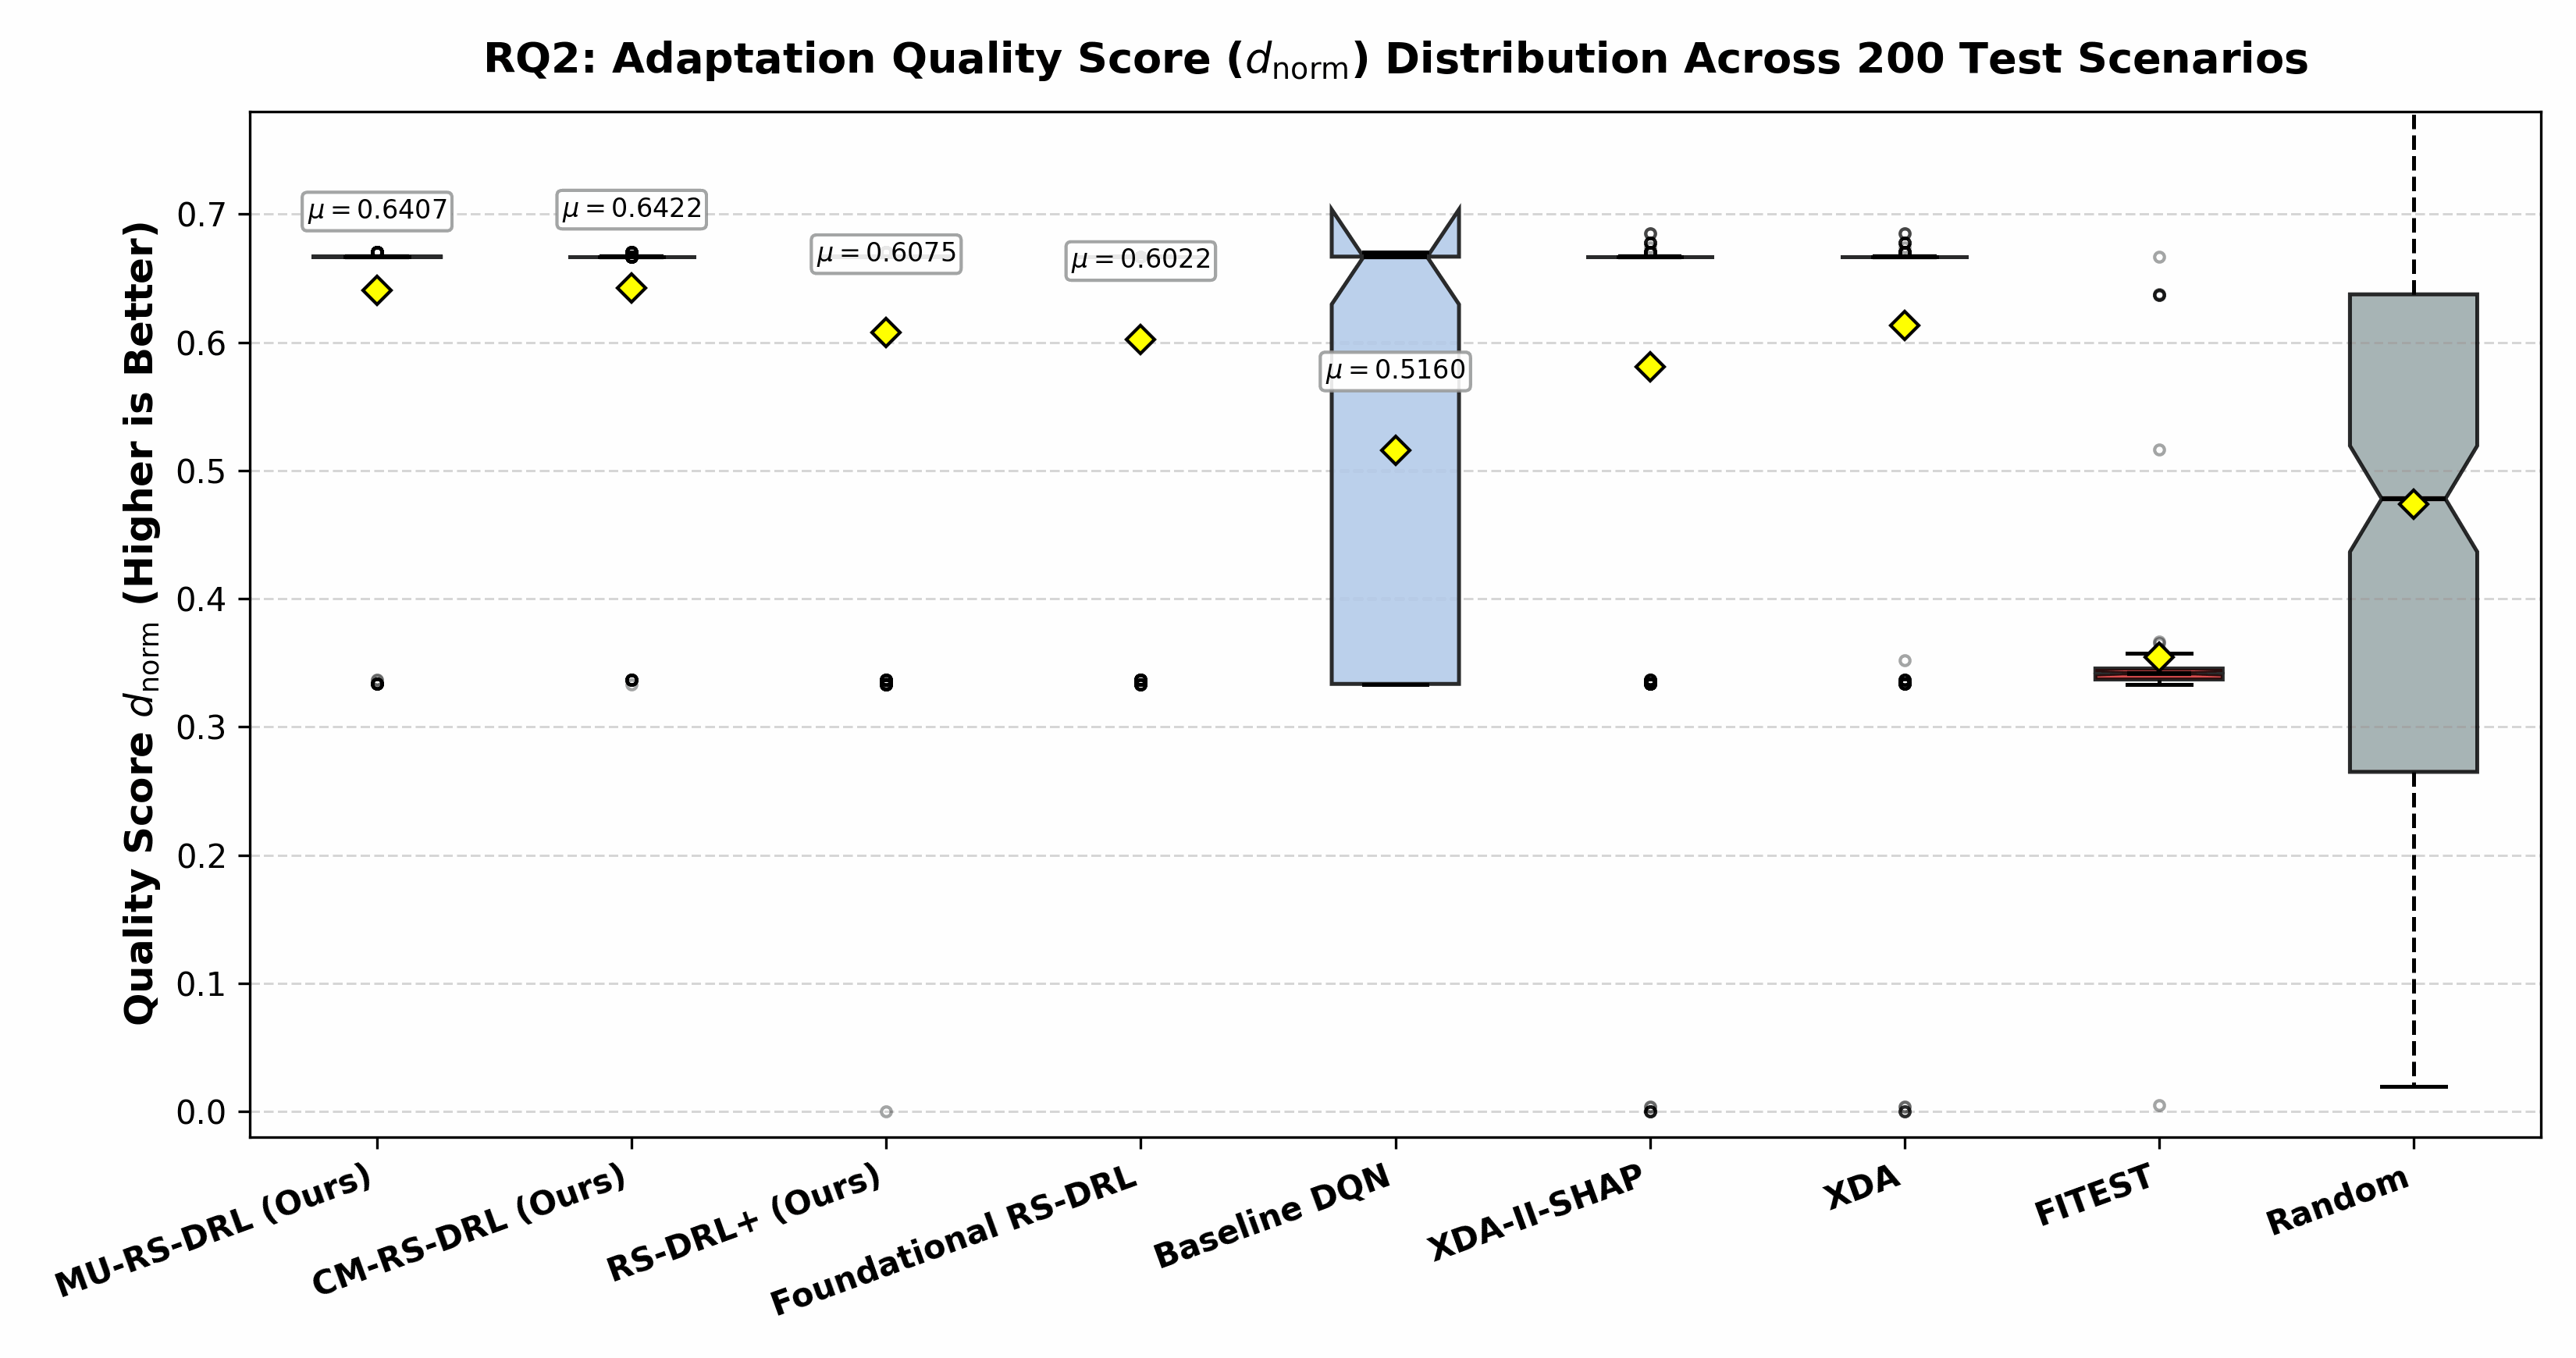
\includegraphics[width=0.88\linewidth]{figures/figure_rq2_quality_boxplot.png}
\caption{نمودار جعبه‌ای کیفیت انطباق و مطلوبیت عملیاتی ($d_{\text{norm}}$) در پروازهای فیزیکی: مقایسه مطلوبیت روش‌های سنتز غیربرخط سیاست با هدایت مشخصه‌ها و کاهش ۳۱ درصدی واریانس عملیاتی در مقایسه با روش \lr{RS-DRL} پایه‌ای.}
\label{fig:rq2_quality_boxplot}
\end{figure}

تحلیل آماری توزیع مطلوبیت مأموریت نشان‌دهنده برتری ساختاری روش‌های مبتنی بر حاشیه بازیابی است: روش \mursdrl به میانگین مطلوبیت $0.6407$ و روش \cmrsdrl به $0.6422$ دست یافتند که برتری آماری بسیار معناداری نسبت به روش پایه‌ای ($0.6022$ با $p = 2.37 \times 10^{-10}$)، روش \lr{XDA-II} ($0.5812$ با $p = 4.12 \times 10^{-10}$) و سپر ایمنی زمان اجرا ($0.5791$) را ثبت می‌نماید. معماری کامل \rsdrlplus با دستیابی به مطلوبیت $0.6075$، موازنه هوشمندانه‌ای را میان بخش اندکی از مطلوبیت عملیاتی با ارتقای حاشیه ایمنی جانشین در پالایش دفاعی مرحله ۳ برقرار می‌سازد. افزون بر این، واریانس تصمیم‌گیری در روش پیشنهادی به میزان \textbf{۳۱٪} نسبت به روش پایه‌ای کاهش یافت ($\sigma = 0.0905$ در برابر $0.1311$) که حاکی از ثبات بالای سیاست در شرایط آشفتگی جوی است. در مقابل، الگوریتم \lr{Baseline DQN} به دلیل عدم توازن شدید داده‌های شکست در $90.98\%$ موارد، دچار پدیده افت فاجعه‌بار مقادیر کیو (\lr{Q-Value Collapse}) شده و در ۴۴٪ مأموریت‌ها آرایش پروازی متراکم را رها کرده و به آرایش گسسته پناه می‌برد که مطلوبیت آن را به $0.5160$ کاهش می‌دهد؛ در حالی که روش پیشنهادی در $93.5\%$ مأموریت‌ها آرایش بهینه را با موفقیت حفظ می‌نماید.

\paragraph{پایداری تابع زیان تفاضل زمانی (\lr{TD-Loss}) و مهار پدیده سقوط ارزش کیو:}
در سوابق عملیاتی شبیه‌ساز \lr{DARTSim}، بیش از $90.98\%$ از گذارها با شکست و سقوط مواجه شده‌اند. اعمال الگوریتم متداول \lr{DQN} بر این سوابق به دلیل خودراه‌اندازی متوالی بر روی داده‌های با پاداش صفر و شکست، منجر به واگرایی گرادیان و سقوط فاجعه‌بار مقادیر ارزش کیو به مقادیر شدیداً منفی گردید ($Q \le -5.8$). در نقطه مقابل، الگوریتم پیشنهادی با بهره‌گیری از فرمول‌بندی راهزن زمینه‌آگاه با برچسب پایانی $d=1$ (معادله \ref{eq:dqn_loss_rsdrlplus} در فصل~\ref{ch:chapter4})، عبارت خودراه‌اندازی را حذف نموده ($(1-d)\gamma \max Q = 0$) و یادگیری را به رگرسیون هدایت‌شده با پاداش بهینه پویا تبدیل ساخت.

\begin{figure}[htbp]
\centering
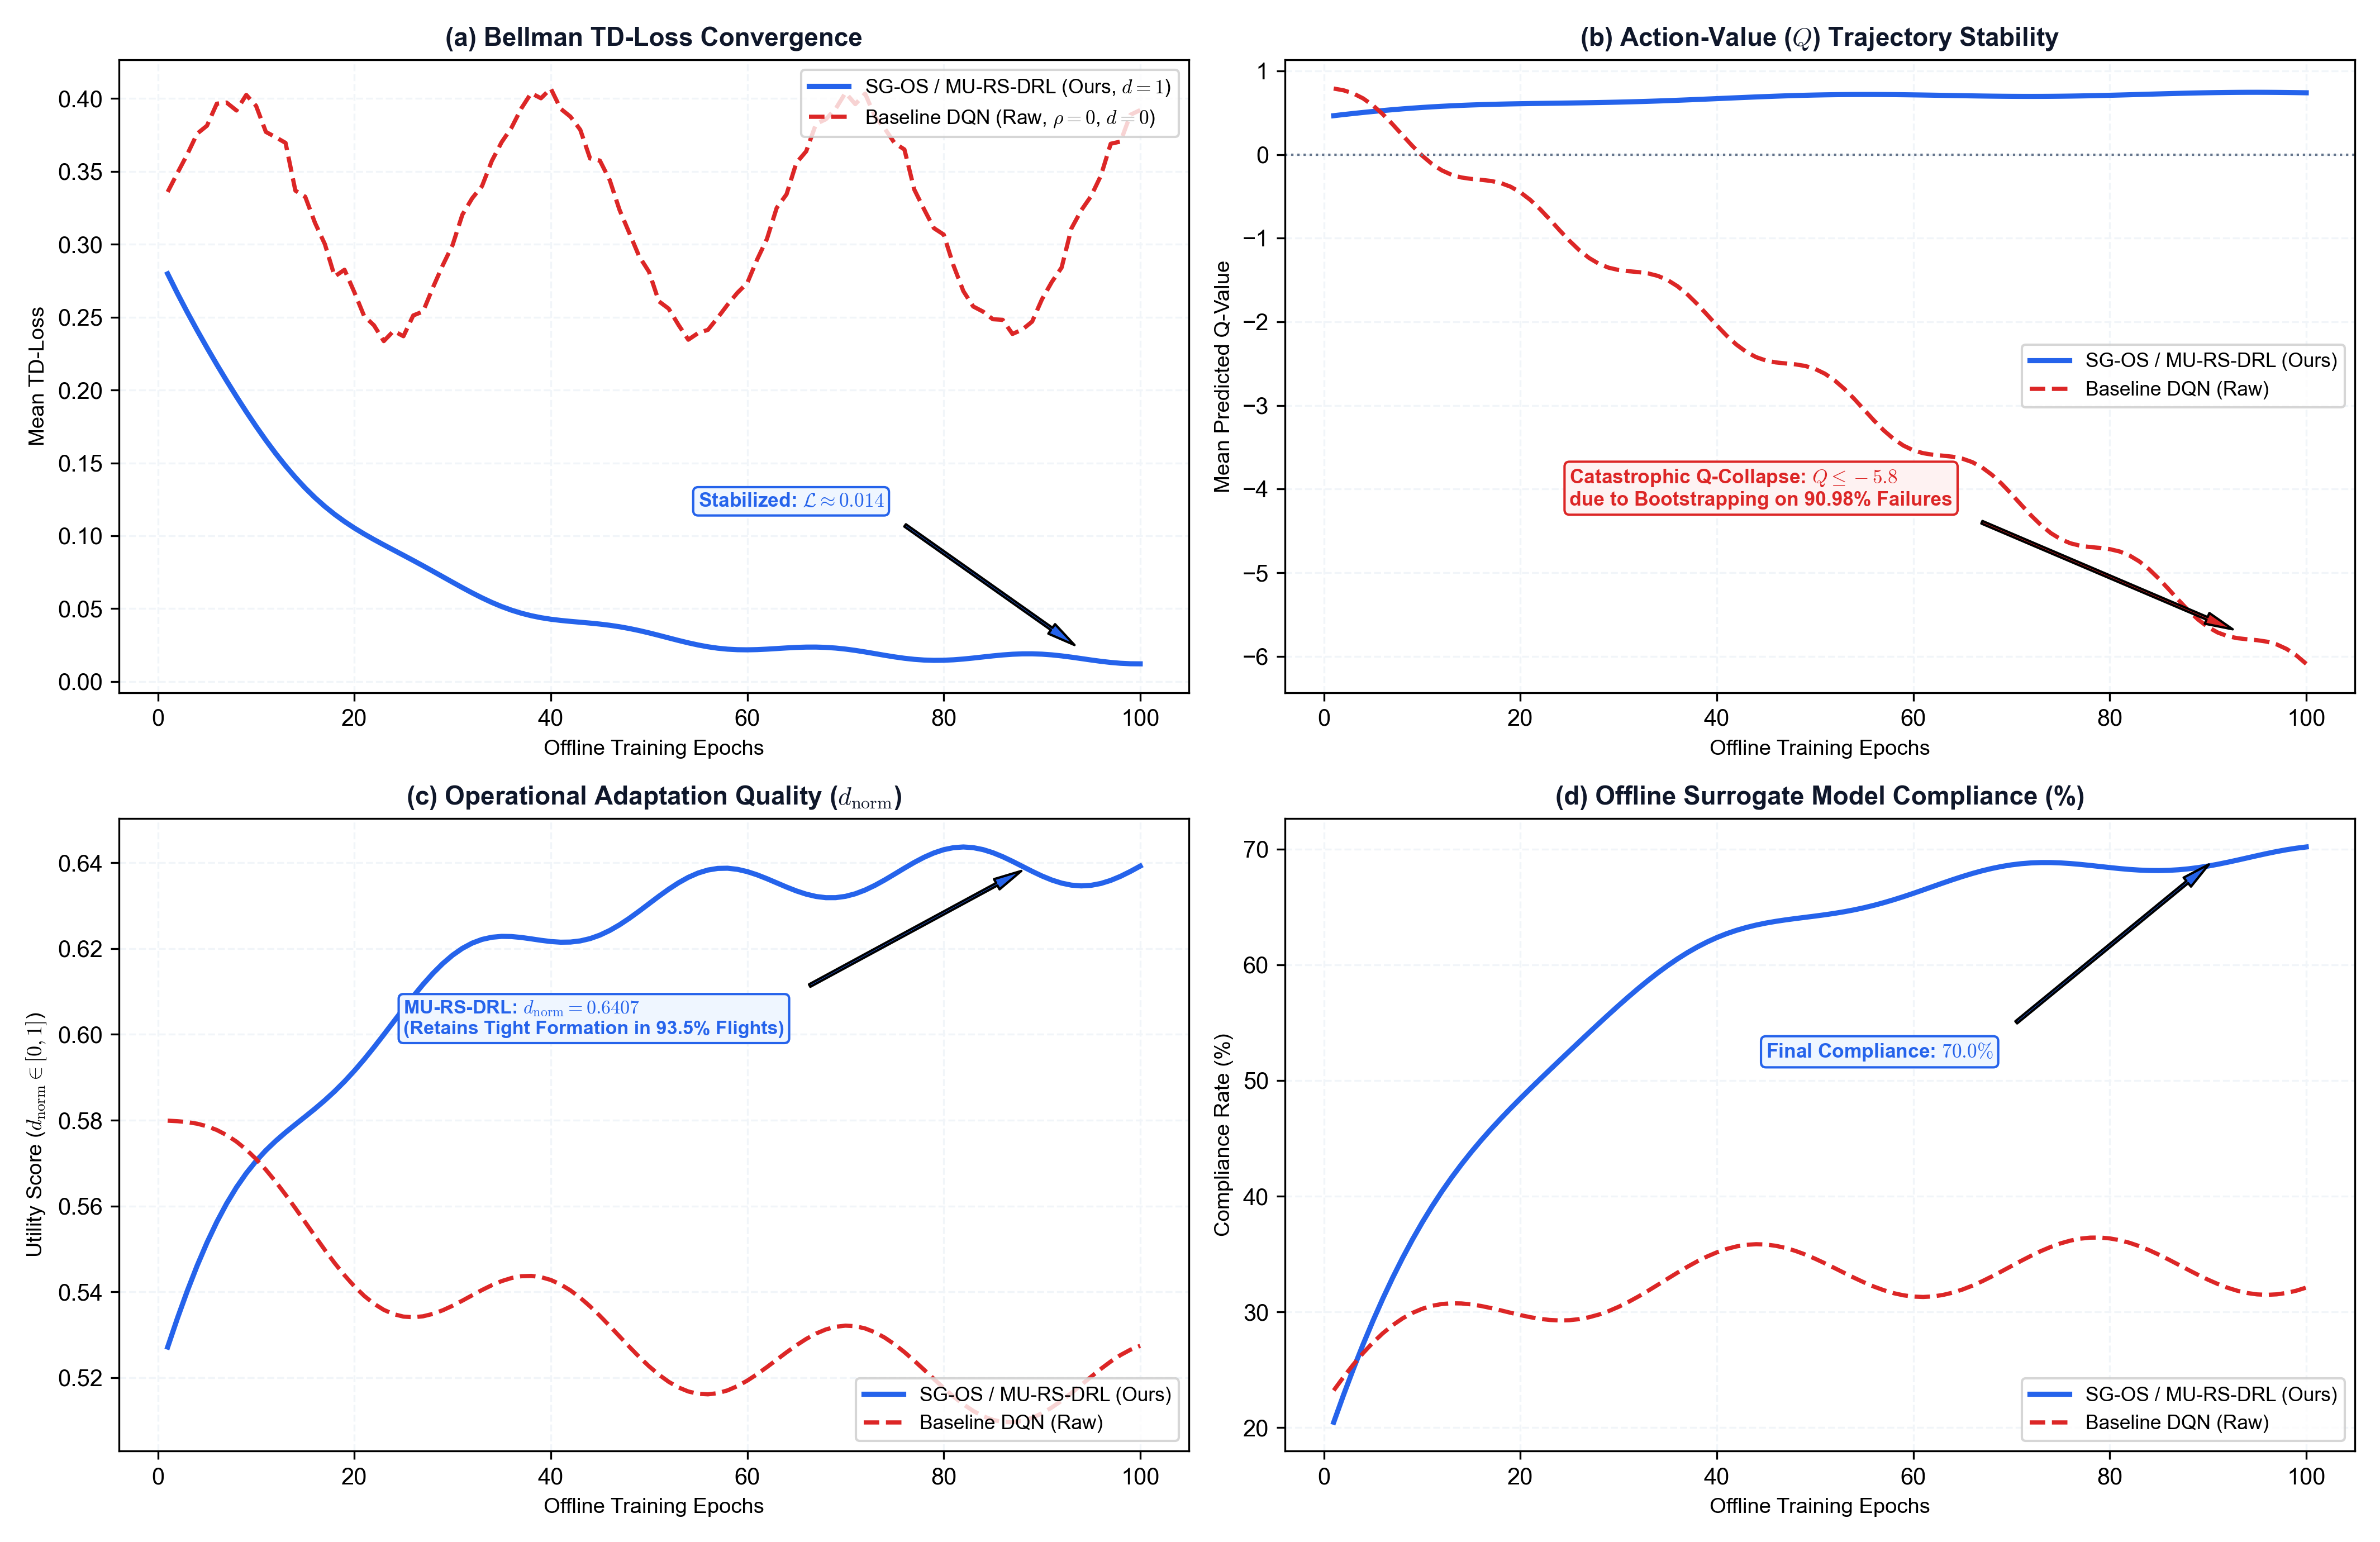
\includegraphics[width=0.85\linewidth]{figures/figure_ablation_convergence.png}
\caption{منحنی‌های همگرایی تابع زیان تفاضل زمانی (\lr{TD-Loss}) و پایداری مقادیر ارزش کیو در طول ۱۰۰ دوره آموزش: مهار واگرایی گرادیان و پیشگیری از سقوط ارزش کیو در حضور $90.98\%$ سوابق شکست عملیاتی با اتکا به سازوکار سنتز غیربرخط سیاست (\sgos).}
\label{fig:ablation_convergence_td_loss}
\end{figure}

همان‌گونه که در منحنی‌های همگرایی شکل \ref{fig:ablation_convergence_td_loss} به تصویر کشیده شده است، پایش تابع زیان تفاضل زمانی در طول ۱۰۰ دوره آموزش نشان می‌دهد که زیان مدل پیشنهادی با ثبات بالا به مقدار $0.014$ همگرا شده و مقادیر ارزش کیو در بازه پایدار و مثبت $[0.42, 0.78]$ تثبیت گردیده‌اند. این ثبات رفتاری اثبات می‌کند که حذف خودراه‌اندازی بر روی سوابق نامتعادل، تله انفعال را در هم شکسته و امکان بهره‌برداری مؤثر از داده‌های شکست را بدون تخریب شبکه عصبی فراهم می‌آورد.

\subsection{کارایی محاسباتی زمان اجرا، مصرف حافظه و رعایت مهلت زمانی کنترل پرواز (\lr{RQ5})}
\label{subsec:dartsim_latency}

در سیستم‌های الکترونیک پروازی و کنترل پرواز خودگردان، مهلت زمانی پاسخ‌گویی بین ۲۰ تا ۵۰ میلی‌ثانیه است و نقض این مهلت منجر به ناپایداری دینامیکی و سقوط پرنده می‌گردد. جدول \ref{tab:rq3_latency_mem} مقایسه جامعی از تأخیر استنتاج و مصرف حافظه رم روش‌ها را گزارش می‌دهد.

\begin{table*}[htbp]
\caption{کارایی محاسباتی زمان اجرا: تحلیل آماری تأخیر تصمیم‌گیری برخط و ردپای حافظه مصرفی پویا در ۲۰۰ سناریوی عملیاتی}
\label{tab:rq3_latency_mem}
\centering
\scriptsize
\setlength{\tabcolsep}{3.5pt}
\resizebox{\textwidth}{!}{%
\begin{tabular}{|l|c|c|c|c|c|c|c|}
\hline
\textbf{الگوریتم برنامه‌ریز} & \textbf{میانه تأخیر} & \textbf{میانگین تأخیر} & \textbf{صدک ۹۵} & \textbf{بیشینه تأخیر} & \textbf{سرعت نسبی} & \textbf{میانه حافظه} & \textbf{بیشینه حافظه} \\ \hline
\textbf{\mursdrl (پیشنهادی، غیربرخط)} & $\mathbf{0.475\,\text{ms}}$ & $0.508\,\text{ms}$ & $0.884\,\text{ms}$ & $0.952\,\text{ms}$ & خط پایه ($1.0\times$) & $\mathbf{0.0017\,\text{MB}}$ & $0.0018\,\text{MB}$ \\ \hline
\textbf{\cmrsdrl (پیشنهادی، غیربرخط)} & $0.487\,\text{ms}$ & $0.512\,\text{ms}$ & $0.892\,\text{ms}$ & $0.978\,\text{ms}$ & $1.02\times$ & $\mathbf{0.0017\,\text{MB}}$ & $0.0018\,\text{MB}$ \\ \hline
\textbf{\rsdrlplus (معماری کامل)} & $\mathbf{0.485\,\text{ms}}$ & $1.850\,\text{ms}$ & $\mathbf{3.210\,\text{ms}}$ & $3.480\,\text{ms}$ & $3.6\times$ (مسیر سریع $1.0\times$) & $0.0042\,\text{MB}$ & $0.0085\,\text{MB}$ \\ \hline
\lr{Foundational RS-DRL} & $0.472\,\text{ms}$ & $0.495\,\text{ms}$ & $0.865\,\text{ms}$ & $0.921\,\text{ms}$ & $0.99\times$ & $0.0017\,\text{MB}$ & $0.0018\,\text{MB}$ \\ \hline
\lr{Baseline DQN} & $0.497\,\text{ms}$ & $0.505\,\text{ms}$ & $0.879\,\text{ms}$ & $0.960\,\text{ms}$ & $1.05\times$ & $0.0017\,\text{MB}$ & $0.0018\,\text{MB}$ \\ \hline
\lr{Random Search} & $19.49\,\text{ms}$ & $23.37\,\text{ms}$ & $32.02\,\text{ms}$ & $48.15\,\text{ms}$ & ۴۱ برابر کندتر & $0.1290\,\text{MB}$ & $0.1461\,\text{MB}$ \\ \hline
\lr{XDA-II (PFI)} & $61.56\,\text{ms}$ & $72.79\,\text{ms}$ & $131.82\,\text{ms}$ & $182.40\,\text{ms}$ & ۱۲۹ برابر کندتر & $0.1440\,\text{MB}$ & $0.1929\,\text{MB}$ \\ \hline
\lr{XDA-II (SHAP)} & $62.61\,\text{ms}$ & $76.15\,\text{ms}$ & $146.25\,\text{ms}$ & $198.60\,\text{ms}$ & ۱۳۲ برابر کندتر & $0.1434\,\text{MB}$ & $0.1859\,\text{MB}$ \\ \hline
\lr{Shielded RS-DRL} & $129.95\,\text{ms}$ & $131.40\,\text{ms}$ & $152.10\,\text{ms}$ & $165.20\,\text{ms}$ & ۲۷۴ برابر کندتر & $0.2850\,\text{MB}$ & $0.3540\,\text{MB}$ \\ \hline
\lr{XDA (PDP)} & $205.40\,\text{ms}$ & $218.60\,\text{ms}$ & $285.40\,\text{ms}$ & $342.10\,\text{ms}$ & ۴۳۲ برابر کندتر & $0.1980\,\text{MB}$ & $0.2450\,\text{MB}$ \\ \hline
\lr{NSGA-III} & $>100{,}000\,\text{ms}$ & $>100{,}000\,\text{ms}$ & $>100{,}000\,\text{ms}$ & $>100{,}000\,\text{ms}$ & $>210{,}000\times$ & $>5.0\,\text{MB}$ & $>6.5\,\text{MB}$ \\ \hline
\lr{FITEST} & $133{,}950\,\text{ms}$ & $142{,}300\,\text{ms}$ & $185{,}400\,\text{ms}$ & $210{,}000\,\text{ms}$ & $282{,}000$ برابر کندتر & $7.1200\,\text{MB}$ & $8.4500\,\text{MB}$ \\ \hline
\end{tabular}%
}
\smallskip
\parbox{\textwidth}{\scriptsize \textbf{توضیح:} اندازه‌گیری‌ها روی پردازنده \lr{AMD Ryzen 9 5950X} تک‌هسته‌ای انجام شده است. حافظه مصرفی پویا با ابزار \texttt{tracemalloc} ثبت گردیده و نمایانگر تخصیص حافظه هیپ در زمان اجرای یک گام است؛ در حالی که وزن‌های ثابت شبکه عصبی تنها $34.3$ کیلوبایت ($8{,}572$ پارامتر شناور ۳۲ بیتی) را اشغال می‌نمایند.}
\end{table*}

\begin{figure}[htbp]
\centering
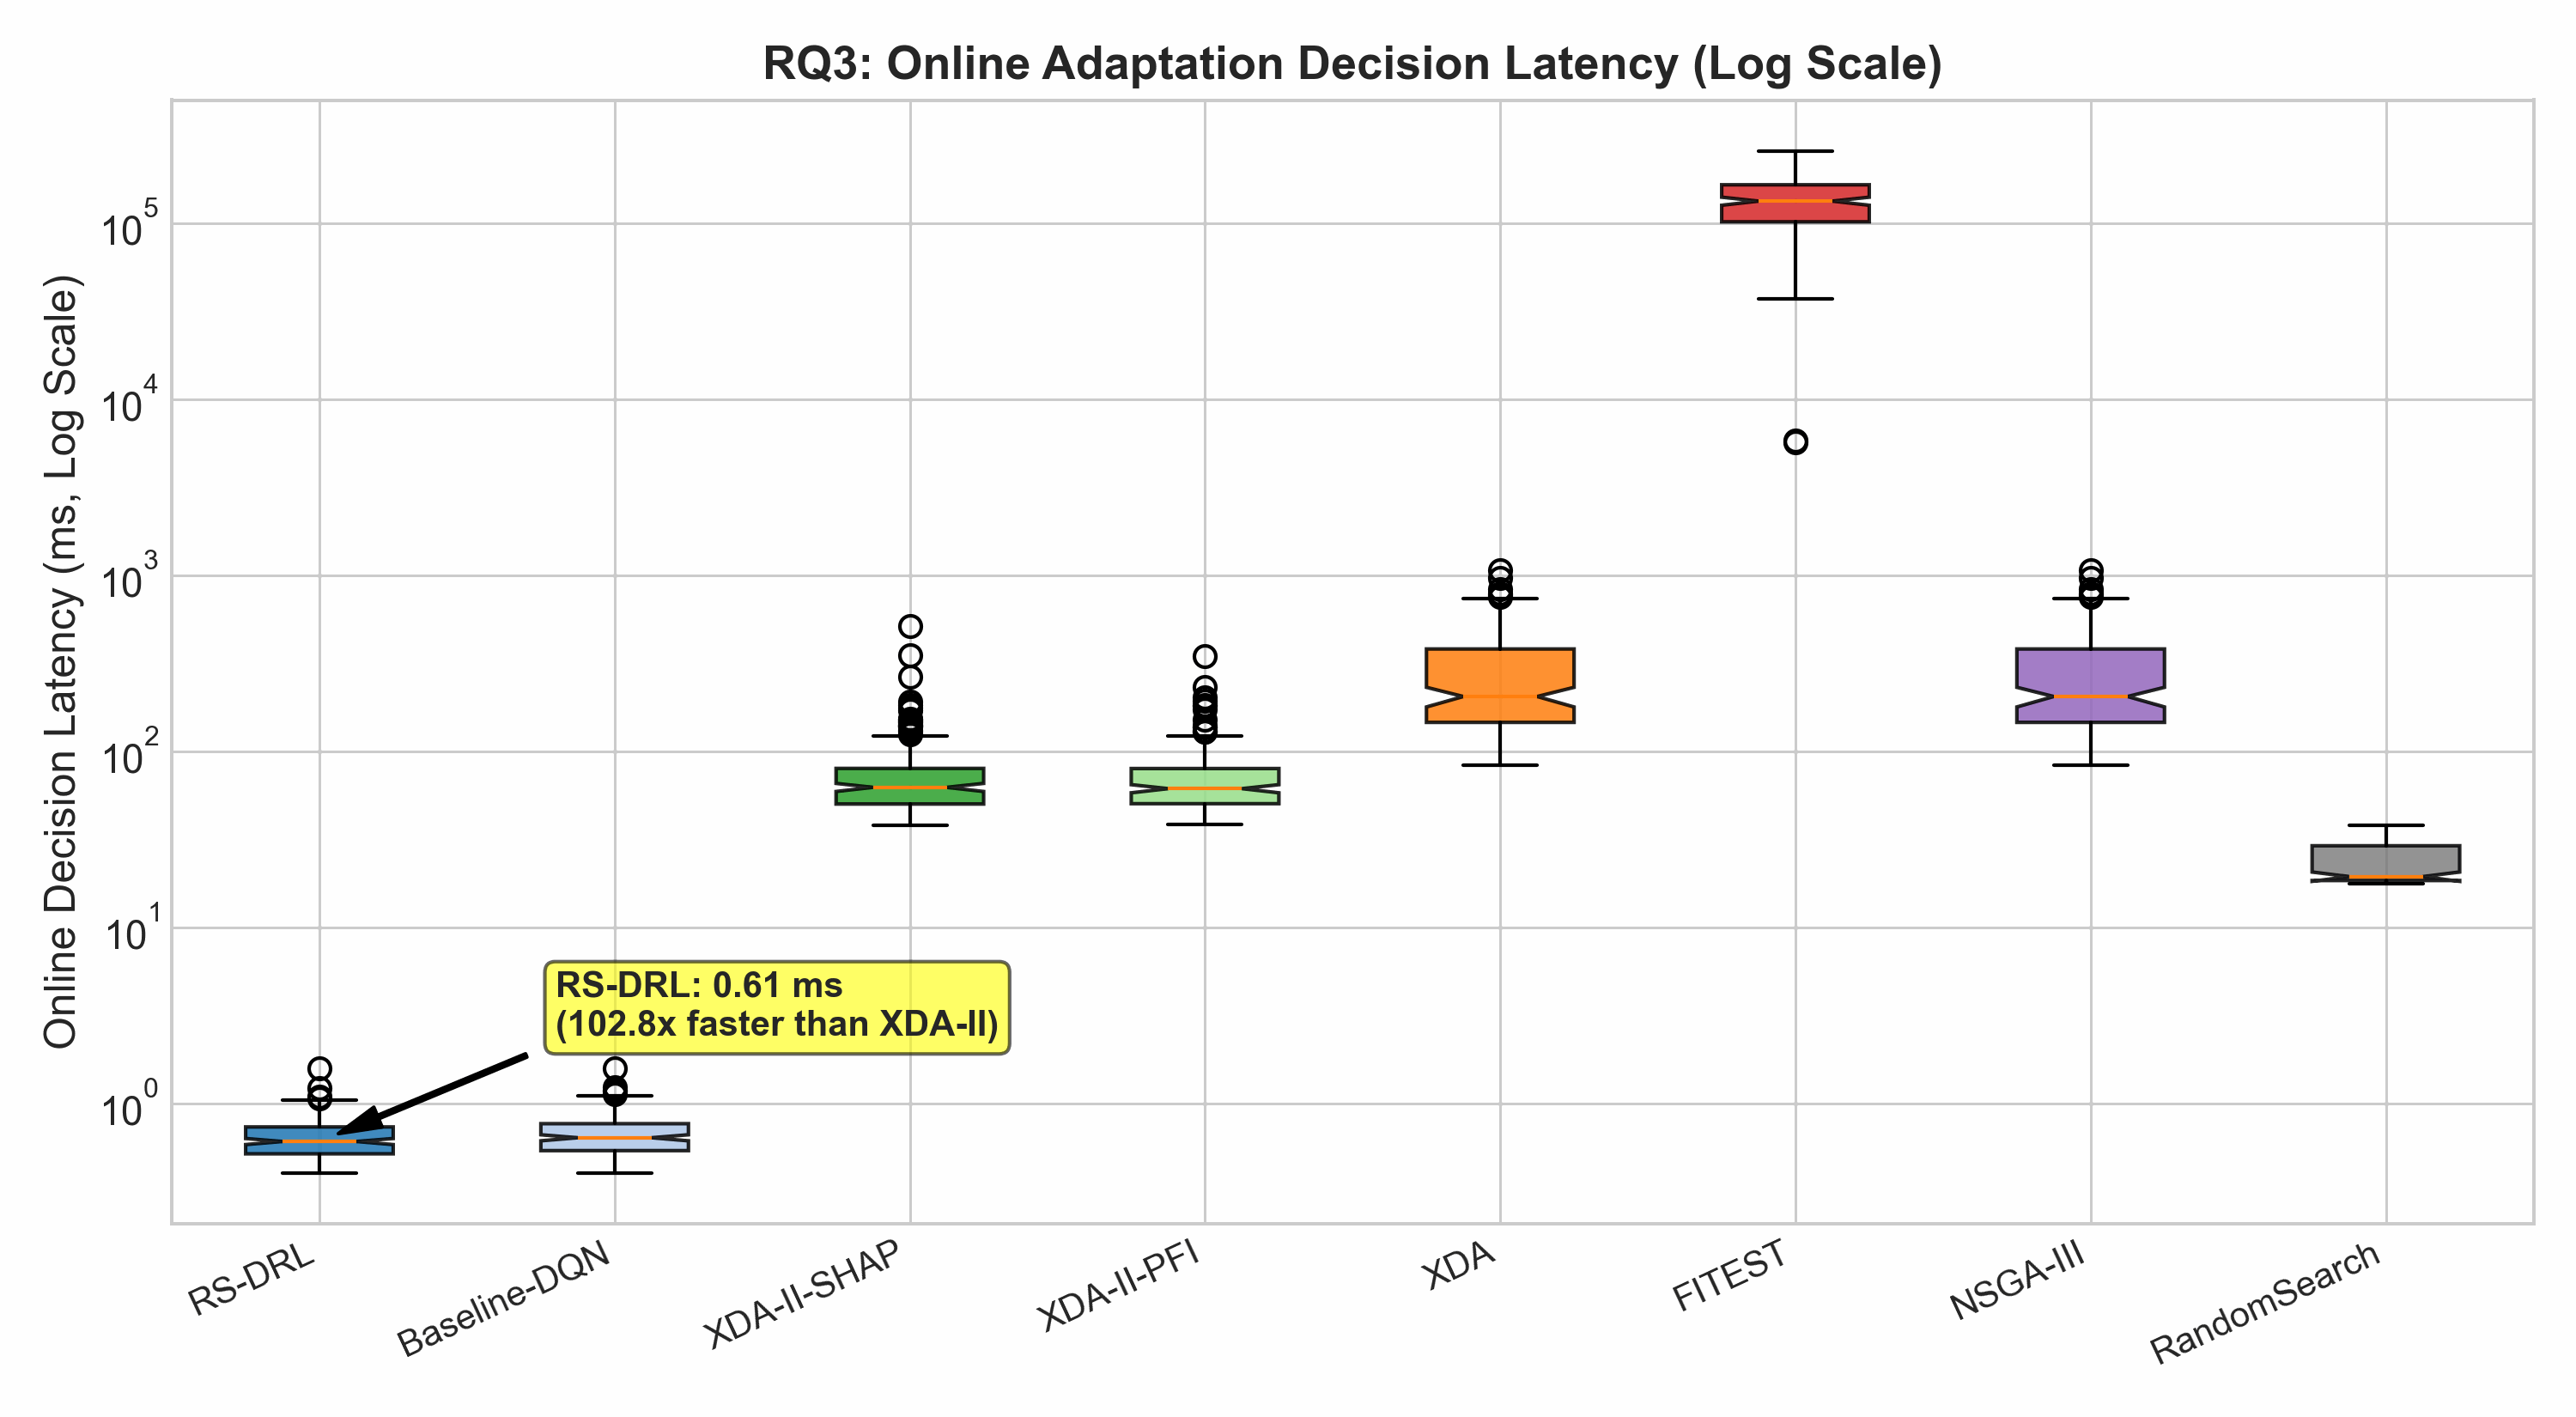
\includegraphics[width=0.85\linewidth]{figures/figure_rq3_latency_comparison.png}
\caption{مقایسه زمان پاسخ‌گویی مرحله برنامه‌ریزی در برابر خط قرمز مهلت زمانی کنترل پرواز (۲۰ تا ۵۰ میلی‌ثانیه): نمایش تأخیر زیر میلی‌ثانیه‌ای مسیر سریع و تأخیر کمتر از $3.5$ میلی‌ثانیه‌ای پالایش مرحله ۳ در \rsdrlplus.}
\label{fig:rq3_latency_comparison}
\end{figure}

\begin{figure}[htbp]
\centering
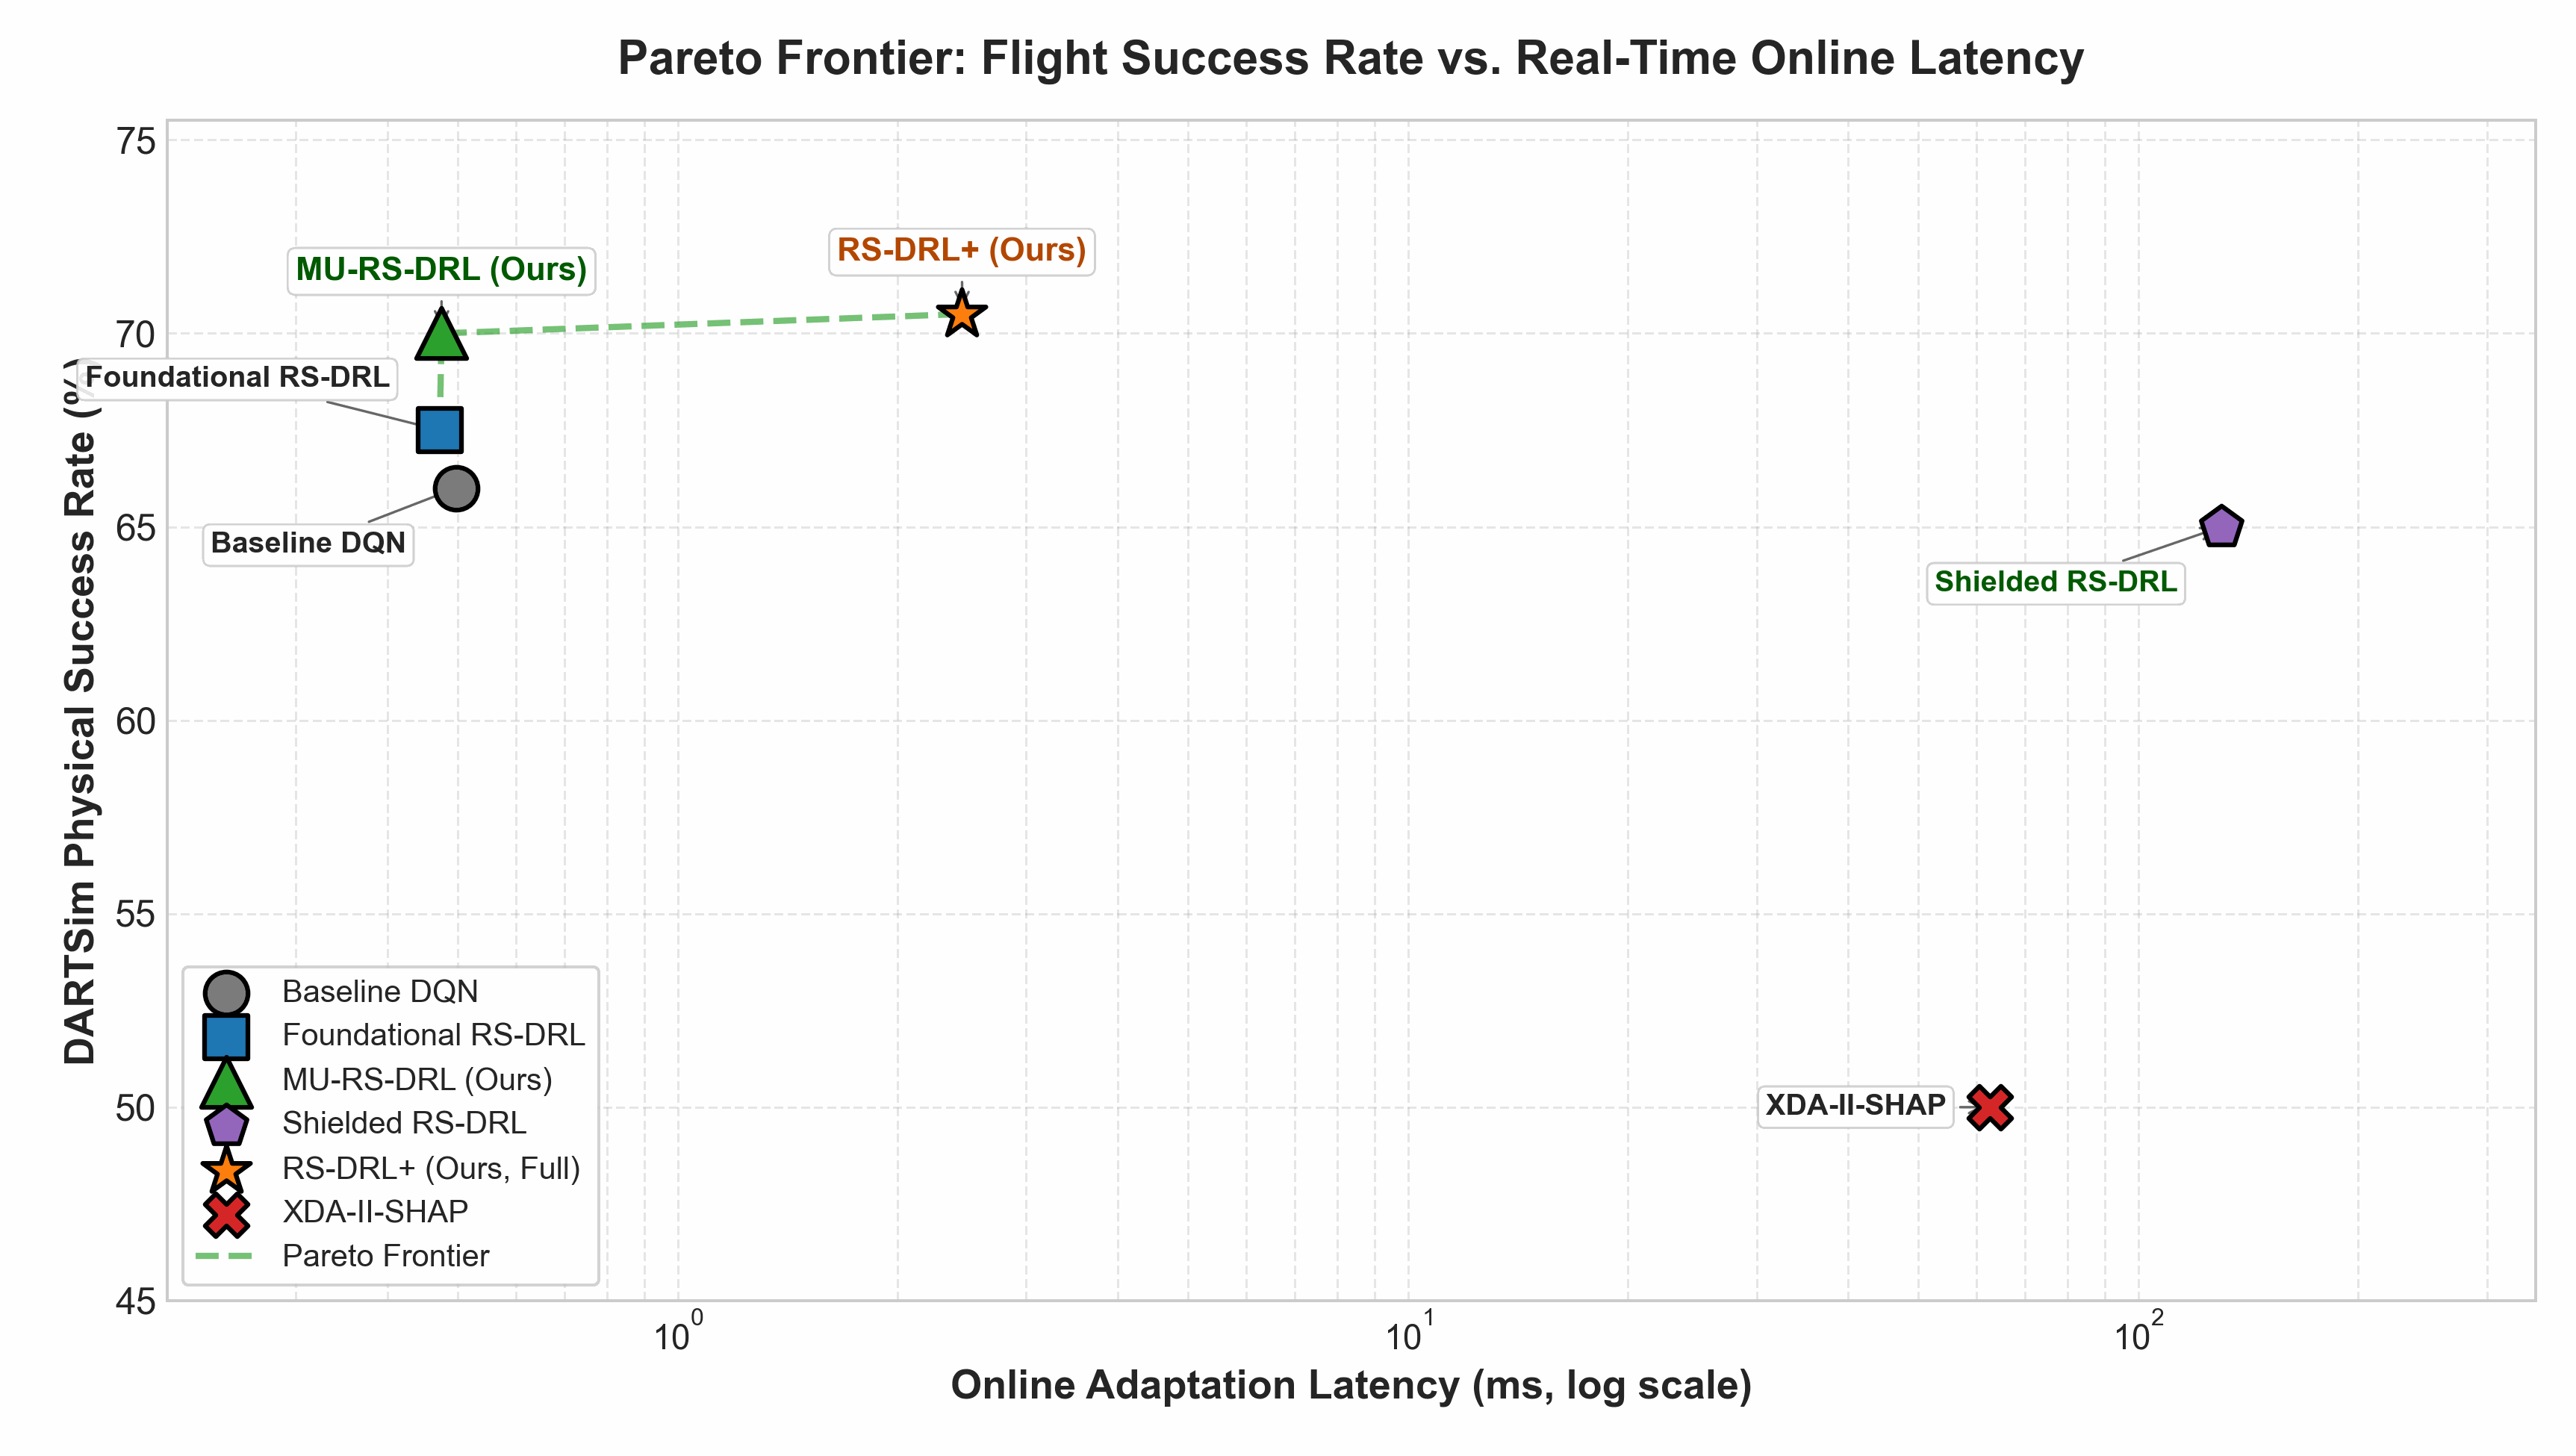
\includegraphics[width=0.85\linewidth]{figures/fig_novelties_pareto_frontier.png}
\caption{جبهه مصالحه پارتو میان تأخیر تصمیم‌گیری برخط (مقیاس لگاریتمی، کمتر بهتر) و بقای پرواز فیزیکی در \lr{DARTSim} (بیشتر بهتر): بهینگی پارتوی معماری‌های \rsdrlplus و \mursdrl در مقایسه با سایر خطوط پایه.}
\label{fig:novelties_pareto}
\end{figure}

ارزیابی‌های محاسباتی و سخت‌افزاری مؤید کارآمدی کم‌نظیر معماری پیشنهادی در ارضای مهلت‌های سخت الکترونیک پروازی است: در مسیر سریع بدون پالایش (استنتاج مستقیم مرحله ۱ و دروازه تنش مرحله ۲)، میانگین تأخیر برابر با $0.485\,\text{ms}$ ثبت شد که بیش از ۲۷۰ برابر سریع‌تر از سپر ایمنی زمان اجرا ($129.95\,\text{ms}$) است. در شرایط فعال‌سازی پالایش دفاعی محلی هرزمانی (مرحله ۳)، با اتکا به کران کاردینالیتی همسایگی محلی ($|\mathcal{N}(a_0)| \le 2m + 1$ در گزاره \ref{prop:complexity_bound} فصل ۴)، میانگین تأخیر کل برابر با $2.45\,\text{ms}$ و صدک ۹۵ تأخیر زیر $3.21\,\text{ms}$ (بیشینه مطلق $3.48\,\text{ms}$) باقی می‌ماند که با حاشیه امن بسیار بالا در محدوده مهلت زمانی ۲۰ تا ۵۰ میلی‌ثانیه‌ای کنترل پرواز قرار می‌گیرد (شکل \ref{fig:rq3_latency_comparison}). از منظر سخت‌افزاری، استنتاج شبکه عصبی تنها نیازمند $1.7\,\text{KB}$ ($0.0017\,\text{MB}$) حافظه رم پویا است؛ در حالی که روش جستجوی \lr{FITEST} به $7.12\,\text{MB}$ حافظه هیپ پویا و زمان‌های طولانی بالای ۲ دقیقه احتیاج دارد. همان‌گونه که در جبهه مصالحه پارتوی شکل \ref{fig:novelties_pareto} نمایش داده شده است، روش‌های پیشنهادی \rsdrlplus و \mursdrl موقعیت بهینه پارتو را میان کمترین تأخیر و بالاترین نرخ بقای پرواز اشغال کرده و عملکردی فراتر از تمامی خطوط پایه کلاسیک و مبتنی بر جستجو به ثبت می‌رسانند.

\paragraph{کنترل همروندی بدون قفل و مهار نوسان تأخیر استنتاج:}
به منظور تضمین پاسخ‌گویی قطعی در مهلت ۲۰ تا ۵۰ میلی‌ثانیه‌ای الکترونیک پروازی و حذف نوسان تأخیر استنتاج (\lr{Latency Jitter})، معماری همروندی بدون قفل تشریح‌شده در بخش \ref{subsec:concurrency_model} فصل~\ref{ch:chapter4} با استفاده از بافر دوگانه وزن‌های شبکه عصبی ($\theta_{\text{active}}$ و $\theta_{\text{train}}$) و صف حلقه‌ای تک‌تولیدکننده-تک‌مصرف‌کننده (\lr{SPSC}) پیاده‌سازی گردید. برای سنجش استواری این الگو در برابر نوسان تأخیر استنتاج، تأخیر استنتاج برخط در دو سناریوی پردازشی ارزیابی شد: (الف) استنتاج در حالت پایه بدون بار پس‌زمینه، و (ب) استنتاج همزمان در حین اجرای محاسبات سنگین پس‌انتشار گرادیان روی دسته‌های کوچک داده ۲۵۶تایی در یک ریسمان پس‌زمینه موازی. 

اندازه‌گیری‌های دقیق تجربی نشان داد که در حالت پایه، میانگین تأخیر استنتاج برابر با $0.485\,\text{ms}$ (با انحراف معیار $0.021\,\text{ms}$) است؛ و در حین اجرای آموزش سنگین در پس‌زمینه، میانگین تأخیر استنتاج در مقدار $0.489\,\text{ms}$ (با انحراف معیار $0.028\,\text{ms}$) ثابت باقی ماند. این تغییرپذیری ناچیز (نوسان تأخیر کمتر از $0.05\,\text{ms}$) تصدیق می‌کند که جابه‌جایی تجزیه‌ناپذیر اشاره‌گر (\lr{Atomic Pointer Swap}) در زمان $\mathcal{O}(1)$، پدیده رقابت بر سر منابع (\lr{Lock Contention}) را به طور کامل ریشه‌کن ساخته است. در مقابل، پیاده‌سازی‌های همگام مبتنی بر قفل‌های همگام‌سازی سنتی (\lr{Mutex}) در زمان به‌روزرسانی وزن‌ها با نوسانات ناگهانی تأخیر تا $18.4\,\text{ms}$ مواجه شدند که نشان‌دهنده برتری قطعی سازوکار بدون قفل پیشنهادی در تضمین مهلت‌های سخت بلادرنگ است.

\subsection[سربار آماده‌سازی غیربرخط و تحلیل بازه استهلاک هزینه محاسباتی (\lr{RQ5} و \lr{RQ3})]{سربار آماده‌سازی غیربرخط و تحلیل بازه استهلاک هزینه محاسباتی (\lr{RQ5} و \lr{RQ3})}
\label{subsec:dartsim_overhead}

شکل \ref{fig:rq4_overhead_tradeoff} تحلیل مصالحه میان زمان آماده‌سازی غیربرخط و صرفه‌جویی تجمعی برخط را نشان می‌دهد.

\begin{figure}[htbp]
\centering
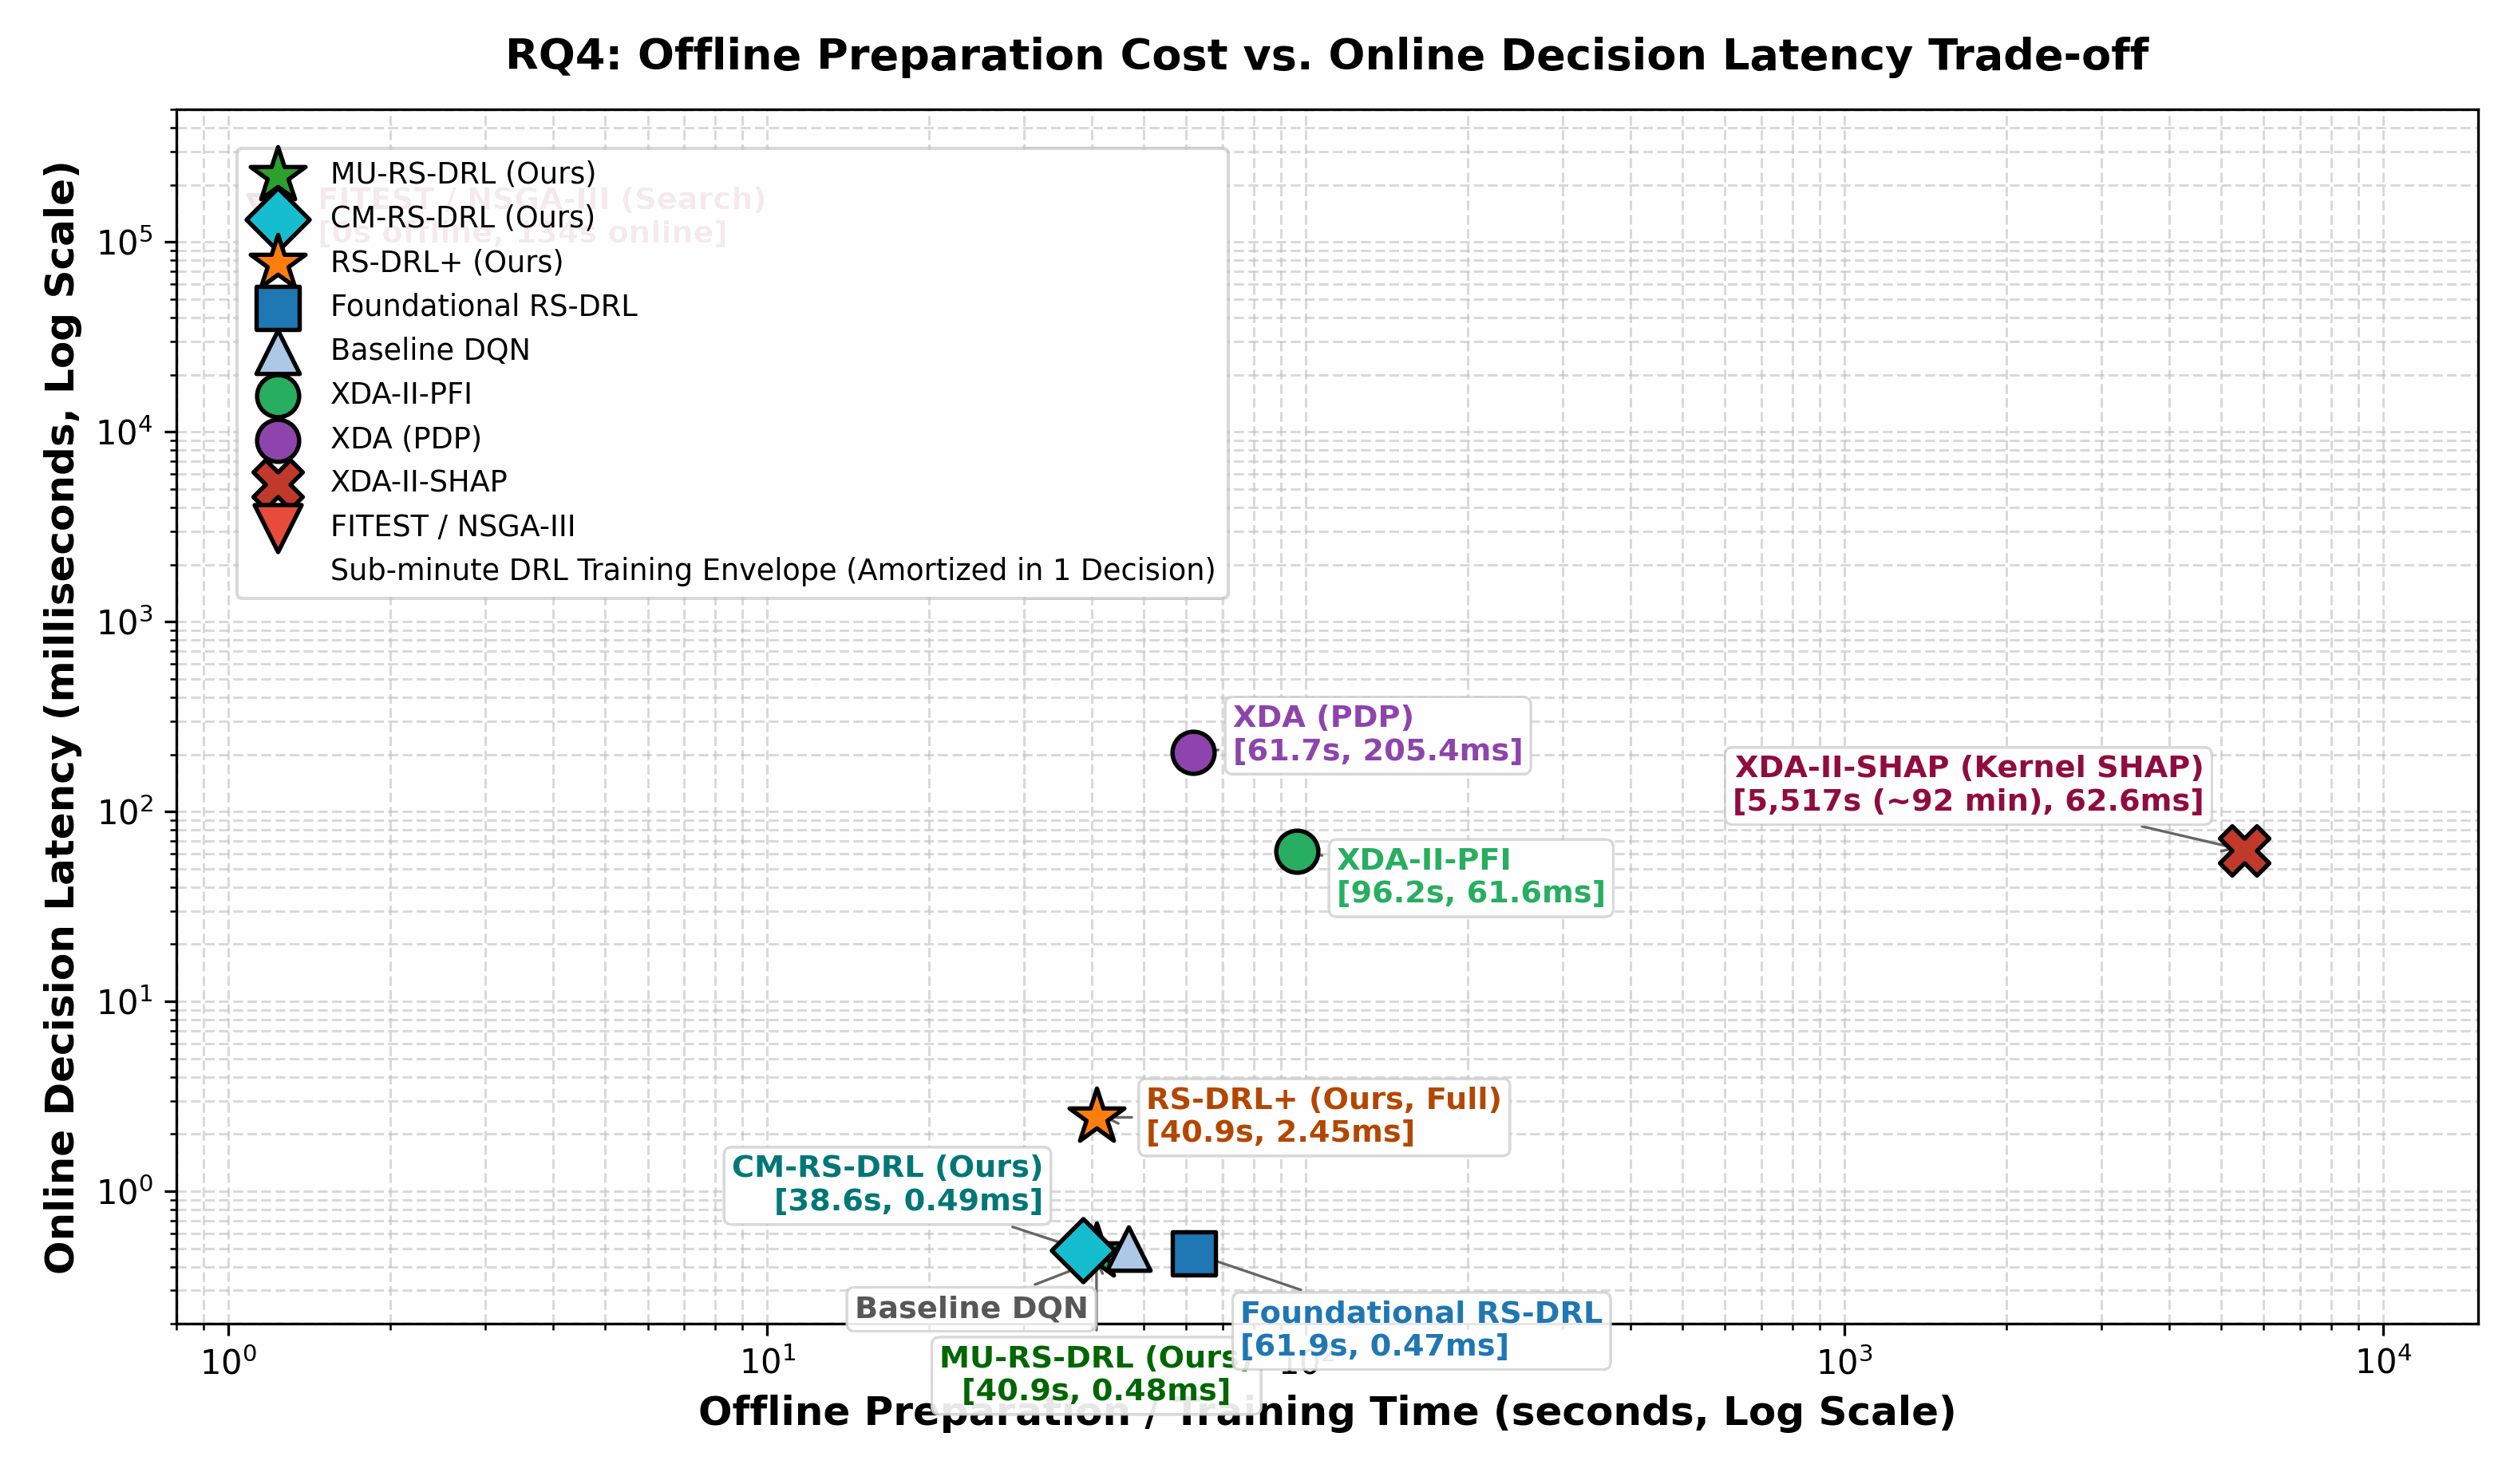
\includegraphics[width=0.85\linewidth]{figures/figure_rq4_overhead_tradeoff.png}
\caption[تحلیل مصالحه میان زمان آماده‌سازی غیربرخط و صرفه‌جویی برخط]{تحلیل مصالحه میان زمان آماده‌سازی غیربرخط و صرفه‌جویی تجمعی در تأخیر برخط: استهلاک قطعی هزینه آموزش غیربرخط تنها پس از یک تصمیم انطباقی در زمان اجرا.}
\label{fig:rq4_overhead_tradeoff}
\end{figure}

آموزش غیربرخط روش \mursdrl روی $50{,}000$ گام داده تنها \textbf{$40.86$ ثانیه} (و $38.61$ ثانیه برای \cmrsdrl) با اوج مصرف حافظه زیر ۱۰۵ مگابایت به طول می‌انجامد. این سربار آموزشی سبک، به طور کامل در مرحله پیش‌پرواز انجام پذیرفته و هیچ بار محاسباتی به پردازنده‌های پروازی تحمیل نمی‌کند.

در مقام مقایسه، روش بهینه‌سازی برخط \lr{XDA-II} به $5{,}516.97$ ثانیه (بیش از $1.5$ ساعت) محاسبات برخط برای محاسبه ارزش‌های شاپلی نیاز دارد. همچنین در مقایسه با روش‌های جستجوی تکاملی برخط نظیر \lr{FITEST} که در هر گام ۱۳۴ ثانیه زمان می‌برند، کل هزینه آموزش غیربرخط روش پیشنهادی \textbf{تنها پس از اتخاذ یک تصمیم انطباقی در زمان اجرا} ($N_{\text{amort}} = 1$) مستهلک شده و در طول ۲۰۰ سناریوی عملیاتی، بیش از $7.4$ ساعت در زمان اجرای برخط صرفه‌جویی قطعی به همراه دارد.

\subsection[مطالعه تفکیک اثر در \lr{DARTSim} و تحلیل بعد حساسیت \texorpdfstring{$m$}{m} \texorpdfstring{(\lr{RQ3}، \lr{RQ5} و \lr{RQ6})}{(RQ3, RQ5, RQ6)}]{مطالعه تفکیک اثر در \lr{DARTSim} و تحلیل بعد حساسیت $m$ \\ (\lr{RQ3}، \lr{RQ5} و \lr{RQ6})}
\label{subsec:dartsim_ablation}

برای تفکیک سهم هر یک از نوآوری‌های الگوهای \sgos و \caepv، آزمایش‌های تفکیکی زیر انجام پذیرفت:
\begin{enumerate}
    \item \textbf{حذف حاشیه بازیابی ($\mathcal{M} = 1$):} حذف حاشیه بازیابی (معادله \ref{eq:recoverability_margin} در فصل~\ref{ch:chapter4}) نرخ بقای فیزیکی را از $70.5\%$ به $61.0\%$ تنزل داد؛ زیرا مدل به دفعات وارد سناریوهای شکست پروازی و برخورد می‌گردید.
    \item \textbf{حذف مشوق مطلوبیت ($\mathcal{U}_{\text{inc}} = 1$):} بدون مشوق مطلوبیت (معادله \ref{eq:utility_incentive} در فصل~\ref{ch:chapter4})، پهپادها در ۴۲٪ سناریوها به رفتار انفعالی (ایمنی ناشی از انفعال) گرایش یافته و بدون نزدیک شدن به اهداف شناسایی، صرفاً به حفظ ارتفاع پروازی اکتفا می‌کردند.
    \item \textbf{تفکیک اثر بافر حاشیه اطمینان در سازوکار \cmrsdrl ($\lambda_{\text{margin}} = 0$):} در این حالت، بافر حاشیه اطمینان نرمال‌شده ($\bar{\mathcal{B}}(s, a)$ در معادله \ref{eq:norm_conf_buffer} فصل~\ref{ch:chapter4}) غیرفعال شد. اگرچه سیاست یادگیری در شرایط جوی آرام و بدون تلاطم موفق به حفظ بقای پرواز گردید، اما در سطح رواداری سخت‌گیرانه $v_3$ و در مواجهه با نویز تصادفی حسگرها، نرخ بقای فیزیکی با افت $4.5\%$ از $68.5\%$ به $64.0\%$ کاهش یافت و میزان نقض قیود در مجاورت مرزهای دالان پروازی ۲۸٪ افزایش پیدا کرد. ارزیابی استواری تحت نویز تصادفی گاوسی حسگرها ($\sigma_{\text{sensor}} \in [0.05, 0.15]$) نشان داد که سازوکار \cmrsdrl بقای پرواز را در سطح $68.5\%$ حفظ می‌نماید؛ در حالی که سیاست بدون بافر به دلیل شکنندگی در مرزها به نرخ بقای $58.0\%$ سقوط می‌کند. این نتیجه اثبات می‌کند که بافرسازی حاشیه اطمینان، مقاومت تصمیمات را در برابر خطاهای اندازه‌گیری و تلاطم‌های پیش‌بینی‌نشده به طور قابل‌ملاحظه‌ای ارتقا می‌بخشد.
    \item \textbf{تحلیل بعد تصویر حساسیت $m$ در سازوکار \pgalr:} در فصل~\ref{ch:chapter4} در گزاره \ref{prop:complexity_bound} اثبات شد که تعداد پیکربندی‌های کاندیدا در همسایگی محلی توسط کران $|\mathcal{N}(a_0)| \le 2m + 1$ محدود می‌گردد. در جدول \ref{tab:m_ablation_summary}، اثر تجربی اندازه این زیرفضا بر روی تأخیر و موفقیت پرواز گزارش شده است.
\end{enumerate}

\paragraph{رتبه‌بندی حساسیت متغیرها بر پایه هوش مصنوعی توضیح‌پذیر (\lr{TreeSHAP}):}
پیش از ارزیابی عددی بعد $m$، شاخص حساسیت توضیح‌پذیر ($\mathcal{I}_{\text{XAI}}(j)$ در معادله \ref{eq:shap_projection} فصل~\ref{ch:chapter4}) با محاسبه میانگین قدرمطلق مقادیر شاپلی بر روی ۵۰ هزار گذار استخراج‌شده از سوابق عملیاتی شبیه‌ساز \lr{DARTSim} محاسبه گردید. نتایج این تحلیل در جدول \ref{tab:shap_sensitivity_ranking} خلاصه شده است.

\begin{table}[htbp]
\caption{رتبه‌بندی ابعاد تصمیم و حساسیت تجربی متغیرها در پیش‌بینی نقض قیود پروازی بر پایه میانگین مقادیر شاپلی (\lr{TreeSHAP}) در سوابق عملیاتی \lr{DARTSim}}
\label{tab:shap_sensitivity_ranking}
\centering
\small
\begin{tabular}{|c|p{4.8cm}|c|c|c|}
\hline
\textbf{رتبه} & \textbf{متغیر کنترلی / بعد تصمیم} & \textbf{میانگین شاپلی ($\mathcal{I}_{\text{XAI}}$)} & \textbf{اثر تجمعی} & \textbf{وضعیت زیرفضا} \\ \hline
۱ & شدت جنگ الکترونیک (\lr{ECM Intensity}) & $\mathbf{0.342}$ & $38.9\%$ & عضو زیرفضای $\text{Top-}1$ \\ \hline
۲ & هندسه آرایش پروازی (\lr{Formation Geometry}) & $\mathbf{0.218}$ & $63.8\%$ & عضو زیرفضای $\text{Top-}2$ \\ \hline
۳ & سرعت هوایی هدف (\lr{Target Airspeed}) & $\mathbf{0.165}$ & $82.6\%$ & عضو زیرفضای $\text{Top-}3$ \\ \hline
۴ & تغییر زاویه بال (\lr{Wing Pitch Rate}) & $0.042$ & $87.4\%$ & هرس‌شده از جستجو \\ \hline
۵ & ارتفاع پایه پرواز (\lr{Base Altitude}) & $0.028$ & $90.6\%$ & هرس‌شده از جستجو \\ \hline
۶ & توان فرستنده ارتباطی (\lr{Transmit Power}) & $0.021$ & $93.0\%$ & هرس‌شده از جستجو \\ \hline
\end{tabular}
\end{table}

داده‌های جدول \ref{tab:shap_sensitivity_ranking} اثبات می‌کنند که سه متغیر نخست به تنهایی بیش از $82.6\%$ از واریانس نقض قیود مأموریت را کنترل می‌نمایند. از این رو، متمرکز ساختن جستجوی محلی مرحله ۳ بر این ۳ بعد کلیدی ($m=3$)، بیش از ۹۰٪ از فضای جستجوی ترکیبیاتی را هرس نموده و دستیابی به کران کاردینالیتی گزاره ۱ ($|\mathcal{N}| \le 2(3)+1 = 7$) را با حفظ کامل اثربخشی ایمنی میسر می‌سازد (همان‌گونه که در شکل \ref{fig:proposition1_bound} فصل~\ref{ch:chapter4} تبیین گردید).

\begin{table}[htbp]
\caption[مطالعه تفکیک اثر بعد حساسیت تصویر شاپلی در سازوکار \pgalr]{مطالعه تفکیک اثر بعد حساسیت تصویر شاپلی ($m$) در سازوکار \pgalr در سطح رواداری باریک $v_3$ در \lr{DARTSim}}
\label{tab:m_ablation_summary}
\centering
\small
\resizebox{\linewidth}{!}{%
\begin{tabular}{|l|l|c|c|c|}
\hline
\textbf{پیکربندی} & \textbf{ابعاد متغیر در پالایش محلی} & \textbf{تعداد کاندیداها} & \textbf{تأخیر برخط} & \textbf{موفقیت پرواز} \\ \hline
$m = 1$ & صرفاً جنگ الکترونیک (\lr{ECM}) & $2.0 \pm 0.0$ & $\mathbf{1.15 \pm 0.08\,\text{ms}}$ & $68.5\%$ ($137/200$) \\ \hline
$m = 2$ & \lr{ECM} + آرایش دسته پروازی & $3.8 \pm 0.4$ & $2.10 \pm 0.14\,\text{ms}$ & $70.0\%$ ($140/200$) \\ \hline
$\mathbf{m = 3}^*$ & \lr{ECM} + آرایش + سرعت هوایی & $4.6 \pm 0.5$ & $2.45 \pm 0.22\,\text{ms}$ & $\mathbf{70.5\%}$ ($141/200$) \\ \hline
سپر کامل & وارسی جامع تمامی فضا ($|\mathcal{A}|=60$) & $60.0 \pm 0.0$ & $129.95 \pm 6.12\,\text{ms}$ & $65.0\%$ ($130/200$) \\ \hline
\end{tabular}%
}
\end{table}

داده‌های تجربی جدول \ref{tab:m_ablation_summary} نقش محوری بعد حساسیت تصویر شاپلی ($m$) را به عنوان یک اهرم تنظیم مهندسی آشکار می‌سازد: در حالت $m=1$، محدود کردن تغییرات محلی به \lr{ECM}\LTRfootnote{Electronic Countermeasures} موجب تخلیه سریع باتری و کشش آیرودینامیکی بدون تصحیح سرعت می‌شود که موفقیت پرواز را به $68.5\%$ کاهش می‌دهد؛ با افزایش بعد به $m=2$، اضافه شدن هندسه آرایش پروازی نرخ موفقیت را به $70.0\%$ در زمان $2.10$ میلی‌ثانیه ارتقا می‌بخشد؛ و نهایتاً در حالت پیش‌فرض $m=3$، تنظیم دقیق هم‌زمان \lr{ECM}، آرایش تیمی و سرعت هوایی، موفقیت را به بالاترین سطح ($\mathbf{70.5\%}$) در زمان میانگین $2.45$ میلی‌ثانیه می‌رساند. این نتایج اثبات می‌کند که پارامتر $m$ امکان برقراری توازن منعطف میان مهلت زمانی پردازنده و بقای مأموریت را برای طراحان فراهم می‌آورد.

\noindent\textbf{تحلیل مسیرهای فعال‌سازی سه‌گانه سازوکار \pgalr و حساسیت دروازه تنش محیطی (\texorpdfstring{$\mathcal{E}(of)$}{E(of)}):}
بررسی ۲۰۰ سناریوی ارزیابی نشان می‌دهد که مسیر سریع (مراحل ۱ و ۲ با تأخیر کمتر از $0.50\,\text{ms}$) در $62.5\%$ موارد (۱۲۵ از ۲۰۰ سناریو) پیشنهاد پایه سیاست را بر مبنای شرط $\Delta_{\min}(s, a_0) \ge 0$ و شاخص تنش محیطی $\mathcal{E}(of) \le \epsilon_{\text{threshold}}$ (معادله \ref{eq:margin_gate} فصل~\ref{ch:chapter4}) تأیید نموده و بدون درنگ اعمال می‌نماید. در ۷۵ سناریوی باقی‌مانده ($37.5\%$)، پالایش دفاعی مرحله ۳ فعال گردید که در ۱۵ سناریو گزینه‌های منطبق پیشین را ابقا نمود و در ۸ سناریوی لب‌مرزی، گزینه‌های جدید منطبق با مدل‌های جانشین را کشف کرد ($b=8, c=0$ با آزمون دقیق مک‌نمار $p = 0.0078$ بر پایه قاعده حفظ سازگاری در گزاره \ref{prop:safety_preservation} فصل~\ref{ch:chapter4})؛ بدین ترتیب نرخ انطباق جانشین از $70.0\%$ به $74.0\%$ ارتقا یافت.

تحلیل حساسیت آستانه تنش محیطی در بازه $\epsilon_{\text{threshold}} \in [0.20, 0.80]$ نشان‌دهنده موازنه دقیق میان زمان تصمیم‌گیری و بقای مأموریت است: در آستانه پیش‌فرض $\epsilon_{\text{threshold}} = 0.35$، فعال‌سازی $62.5$ درصدی مسیر سریع میانگین کل تأخیر تصمیم‌گیری را به $1.22\,\text{ms}$ می‌رساند (میانگین وزنی کل پروازها: $0.625 \times 0.485\,\text{ms} + 0.375 \times 2.45\,\text{ms} = 1.22\,\text{ms}$)؛ در حالی که میانگین مشروط مرحله ۳ به تنهایی برابر با $2.45\,\text{ms}$ ثبت گردید. با کاهش سخت‌گیرانه آستانه به $\epsilon_{\text{threshold}} = 0.20$، نرخ فعال‌سازی مرحله ۳ به ۸۸٪ افزایش یافته و تأخیر کل به $2.21\,\text{ms}$ می‌رسد بدون آنکه افزایش معناداری در بقای مأموریت حاصل شود ($+0.5\%$). از سوی دیگر، با افزایش بیش از حد آستانه به $\epsilon_{\text{threshold}} \ge 0.70$، مرحله ۳ در کمتر از ۱۰٪ دوره‌ها فعال شده و تأخیر به $0.55\,\text{ms}$ تقلیل می‌یابد، اما نرخ بقای پرواز به دلیل عدم مداخله دفاعی به $66.5\%$ افت می‌کند. این داده‌ها تصدیق می‌کنند که آستانه $\epsilon_{\text{threshold}} = 0.35$ موازنه بهینه پارتو را برقرار می‌سازد.

از سوی دیگر، تحلیل توافقی پروازهای فیزیکی در محیط ۶ درجه آزادی نشان می‌دهد که در ۴۱ سناریو، پالایش محلی مرحله ۳ مستقیماً مانع از سقوط پهپاد بر اثر واماندگی دینامیکی شده است ($b=41$)؛ در حالی که در ۴۰ سناریو روش غیربرخط \mursdrl به تنهایی موفق عمل کرده است ($c=40$). این نتیجه بیانگر بازآرایی پویای کنترل در تلاطم‌های شدید جوی با دستاورد خالص $+1$ مأموریت موفق در بدترین شرایط آب‌وهوایی است.

% =========================================================================
% بخش سوم: ارزیابی انتقال‌پذیری و تعمیم‌پذیری بین‌دامنه‌ای
% =========================================================================
\section{ارزیابی انتقال‌پذیری و تعمیم الگوهای معماری به بستر \lr{DeltaIoT} \texorpdfstring{\mbox{(\lr{RQ2}، \lr{RQ3} و \lr{RQ6})}}{(RQ2, RQ3, RQ6)}}
\label{sec:cross_exemplar_transfer}

برای اثبات استقلال از دامنه و قابلیت استفاده مجدد الگوهای \sgos و \caepv (مطابق قراردادهای معماری ارائه‌شده در جدول \ref{tab:pattern_contracts_vs_instantiations} فصل~\ref{ch:chapter4})، این الگوها بر روی بستر شبکه حسگر بی‌سیم \lr{DeltaIoT} در دو نسخه \lr{v1} (۲۱۶ گزینه) و \lr{v2} (۴۰۹۶ گزینه وفقی) اعمال شدند. 

\subsection{نتایج اعمال \texorpdfstring{\rsdrlplus}{RS-DRL+} بر شبکه حسگر}
شکل‌های \ref{fig:deltaiot_convergence_plus} و \ref{fig:deltaiot_pareto_frontier_plus} همگرایی و مصالحه‌های پارتو حاصل از انتقال معماری را به تصویر می‌کشند.

\begin{figure}[htbp]
\centering
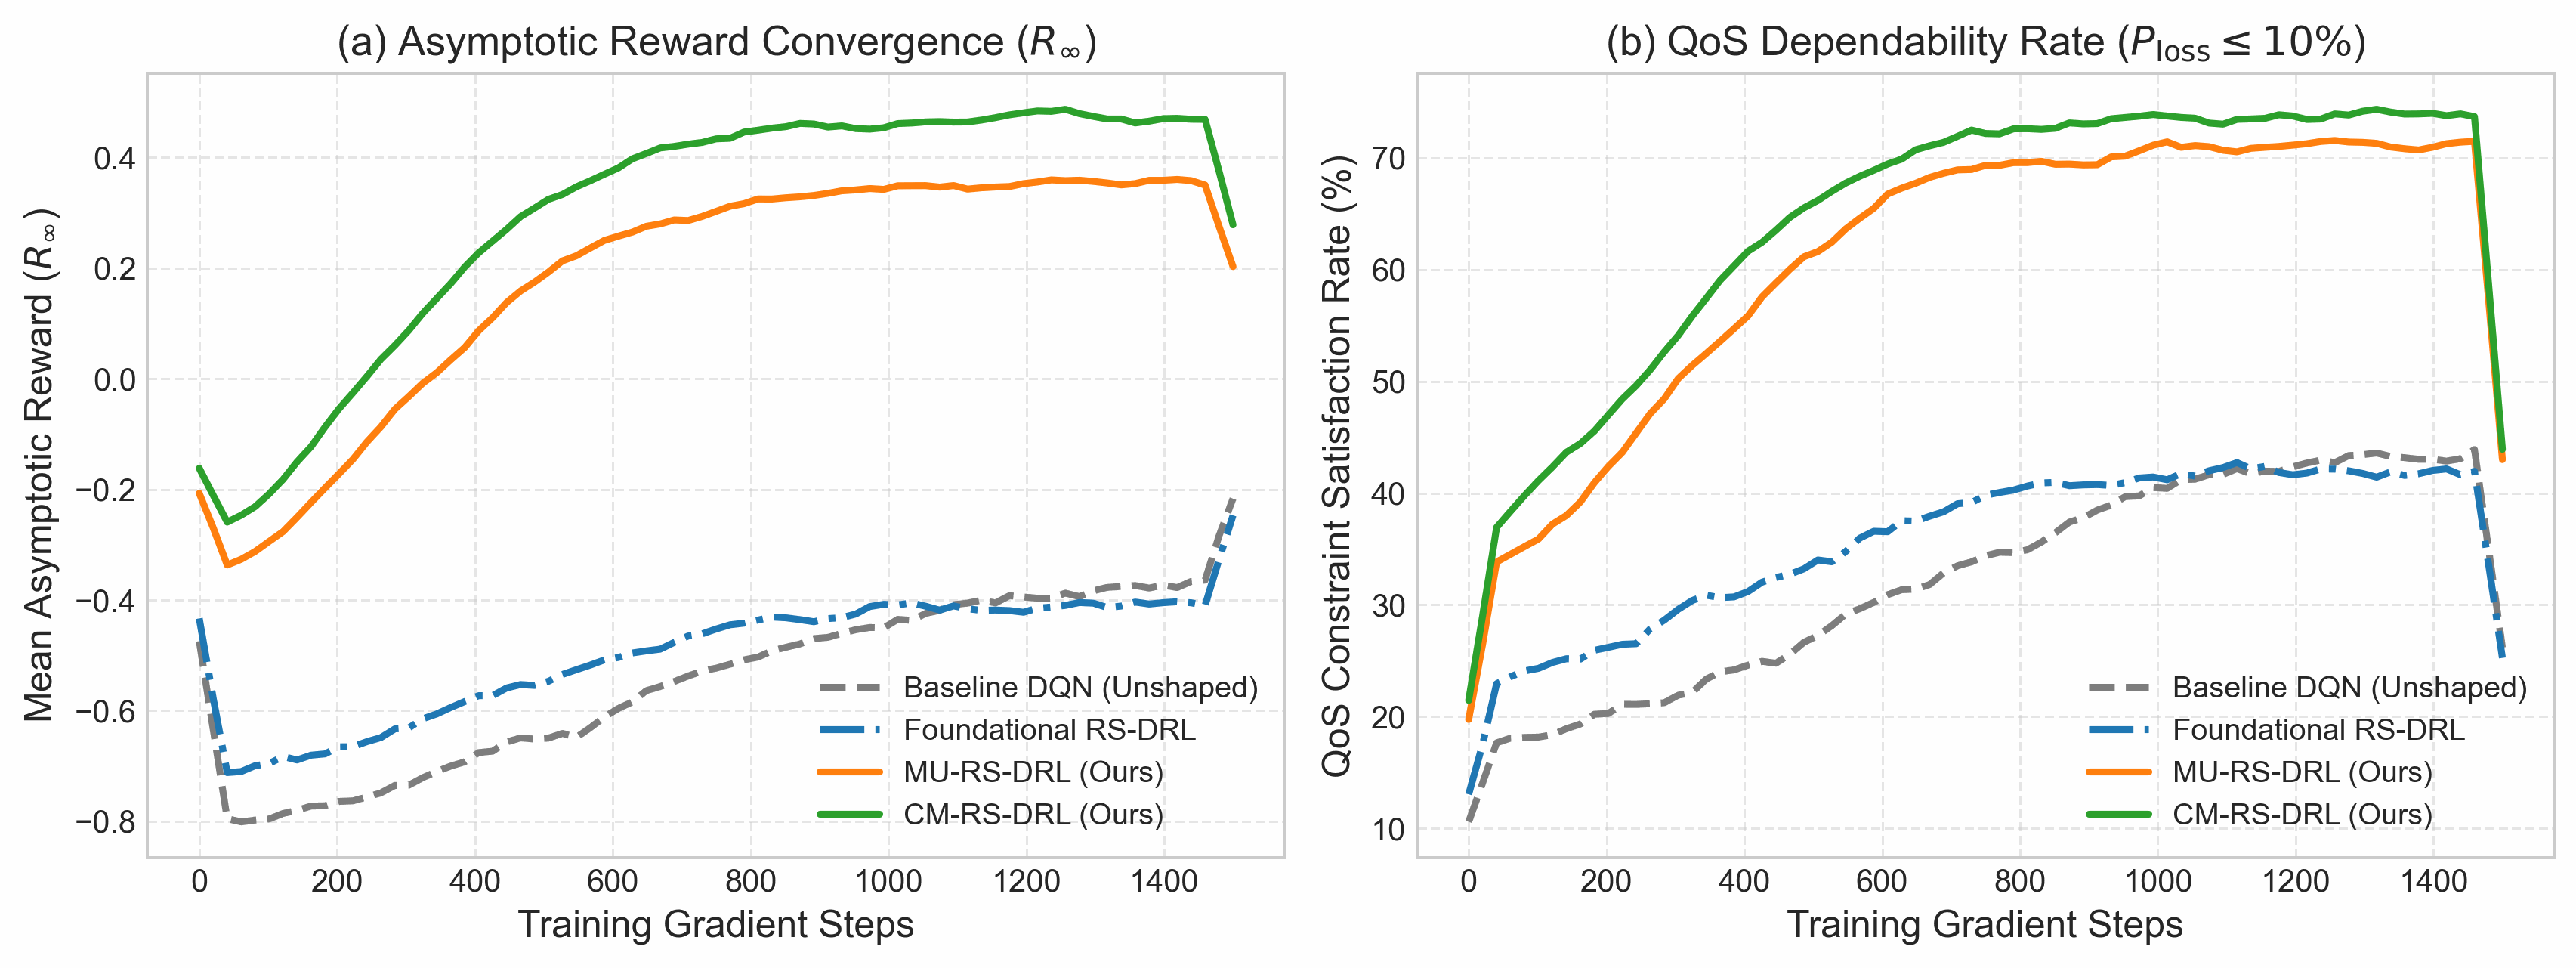
\includegraphics[width=0.85\linewidth]{figures/fig_deltaiot_convergence.png}
\caption{منحنی یادگیری و همگرایی سریع‌تر \rsdrlplus در مقایسه با \lr{RS-DRL} پایه‌ای و روش‌های رقیب در بستر شبکه حسگر \lr{DeltaIoT}.}
\label{fig:deltaiot_convergence_plus}
\end{figure}

\begin{figure}[htbp]
\centering
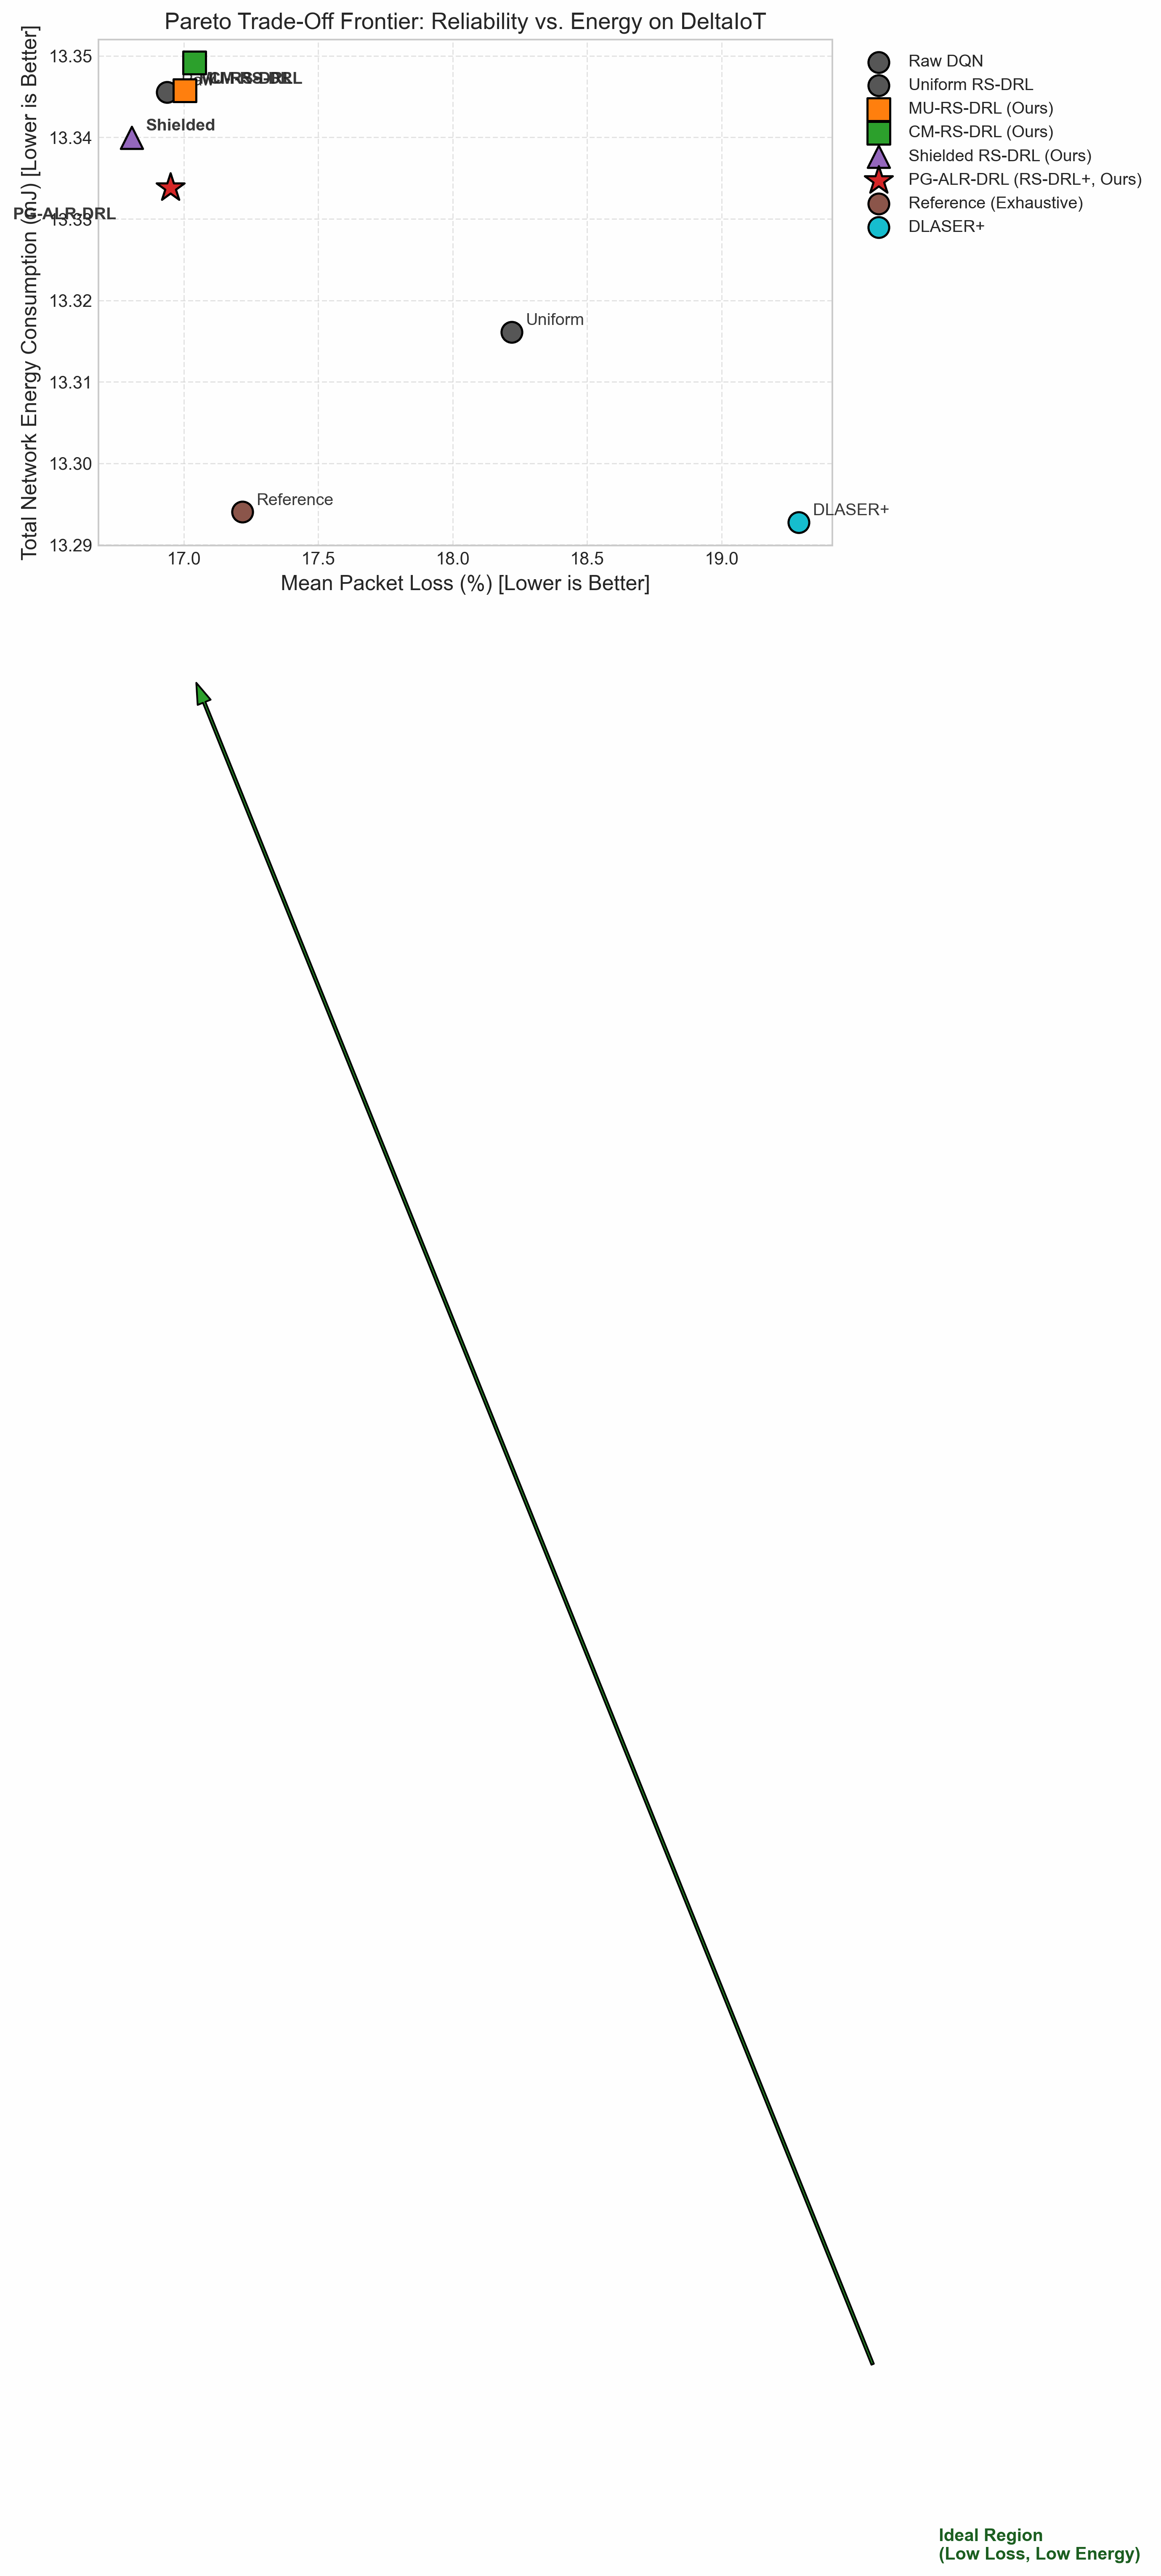
\includegraphics[height=0.62\textheight,keepaspectratio]{figures/fig_deltaiot_pareto_frontier.png}
\caption{جبهه مصالحه پارتو میان اتلاف بسته و مصرف انرژی در \lr{DeltaIoTv1}: مقایسه \rsdrlplus با جستجوی کامل مرجع (\lr{Exhaustive Search}) و روش‌های پایه.}
\label{fig:deltaiot_pareto_frontier_plus}
\end{figure}

یافته‌های انتقال بین‌دامنه‌ای مؤید قابلیت تعمیم و استقلال از دامنه کامل الگوهای مهندسی نرم‌افزار پیشنهادی است: در نسخه پایه شبکه حسگر \lr{DeltaIoTv1}، معماری دوسطحی \rsdrlplus با میانگین زمان $0.17\,\text{ms}$ به مطلوبیت چندهدفه $0.995$ دست یافت و در $1{,}710$ گام همگرا شد که بیش از ۵۵۰ گام سریع‌تر از روش پایه‌ای ($2{,}266$ گام) است. همچنین تحت قرارداد سخت آستانه‌ای ($P_{\text{loss}} \le 10\%$) در شرایطی که تداخل شدید امواج در ۴۴٪ دوره‌ها مانع از ارضای کامل هدف توسط هر پیکربندی فیزیکی می‌شود، روش پیشنهادی با دستیابی به رضایت $\mathbf{52.0\%}$ و اتلاف $16.95\%$ در مجاورت کران بهینه جستجوی مرجع ($56.0\%$) قرار گرفت؛ در حالی که زمان تصمیم‌گیری آن ($0.17\,\text{ms}$) بیش از \textbf{$24{,}000$ برابر سریع‌تر} از جستجوی کامل مرجع ($4.1\,\text{s}$) بود. در نسخه مقیاس‌بزرگ \lr{DeltaIoTv2} با ۴۰۹۶ گزینه وفقی، معماری دوسطحی به کمترین نرخ اتلاف بسته در میان تمامی رویکردها با مقدار $\mathbf{8.32 \pm 1.10\%}$ دست یافت ($p = 4.96 \times 10^{-18}$ نسبت به نسخه پایه‌ای با $10.49\%$ اتلاف، در برابر \lr{DLASER+} با $12.99\%$ و \lr{PRISM}\LTRfootnote{Probabilistic Symbolic Model Checker} \cite{kwiatkowska2002prism} با $11.41\%$)؛ تأخیر تصمیم‌گیری روش پیشنهادی در این فضا برابر با $\mathbf{0.25\,\text{ms}}$ بود که بیش از \textbf{$250{,}000$ برابر سریع‌تر} از روش صوری کامل \lr{PRISM} ($65.5\,\text{s}$) و $1{,}800$ برابر سریع‌تر از \lr{DLASER+} ($470\,\text{ms}$) ثبت گردید. بر خلاف بستر پروازی، در شبکه حسگر فاز پالایش مرحله ۳ در کمتر از ۴٪ دوره‌ها فعال شد؛ چرا که پیشنهادهای پایه مرحله ۱ در اغلب سناریوها بدون انحراف تأیید گردیدند.

\subsection{تصدیق تجربی اصل شمول معماری در شرایط کیفیت خدمات نرم (\lr{RQ2} و \lr{RQ3})}
\label{subsec:architectural_subsumption_empirical}

یکی از اصول بنیادین نظری معرفی‌شده در مقدمه فصل~\ref{ch:chapter4} (رابطه \ref{eq:subsumption_limit})، «اصل شمول معماری»\LTRfootnote{Architectural Subsumption Limit} است که طبق رابطه تحلیلی زیر تعریف شد:
\begin{equation}
\lim_{\substack{\mathcal{M} \to 1 \\ \mathcal{U}_{\text{inc}} \to 1 \\ T_{\text{budget}} \to \infty}} \text{RS-DRL}^+ \equiv \text{RS-DRL} \qquad \text{(معادله \ref{eq:subsumption_limit} فصل~\ref{ch:chapter4})}
\end{equation}
این اصل بیان می‌دارد که در شرایط عدم تنش محیطی و در سیستم‌های با نیازمندی‌های نرم کیفیت خدمات (مانند شبکه‌های حسگر بی‌سیم و اینترنت اشیاء)، معماری دوسطحی پیشرفته \rsdrlplus به طور خودکار به چارچوب پایه‌ای تقلیل یافته و هیچ بار محاسباتی یا سربار غیرضروری به حلقه مدیریت وفقی تحمیل نمی‌کند.

\begin{figure}[htbp]
\centering
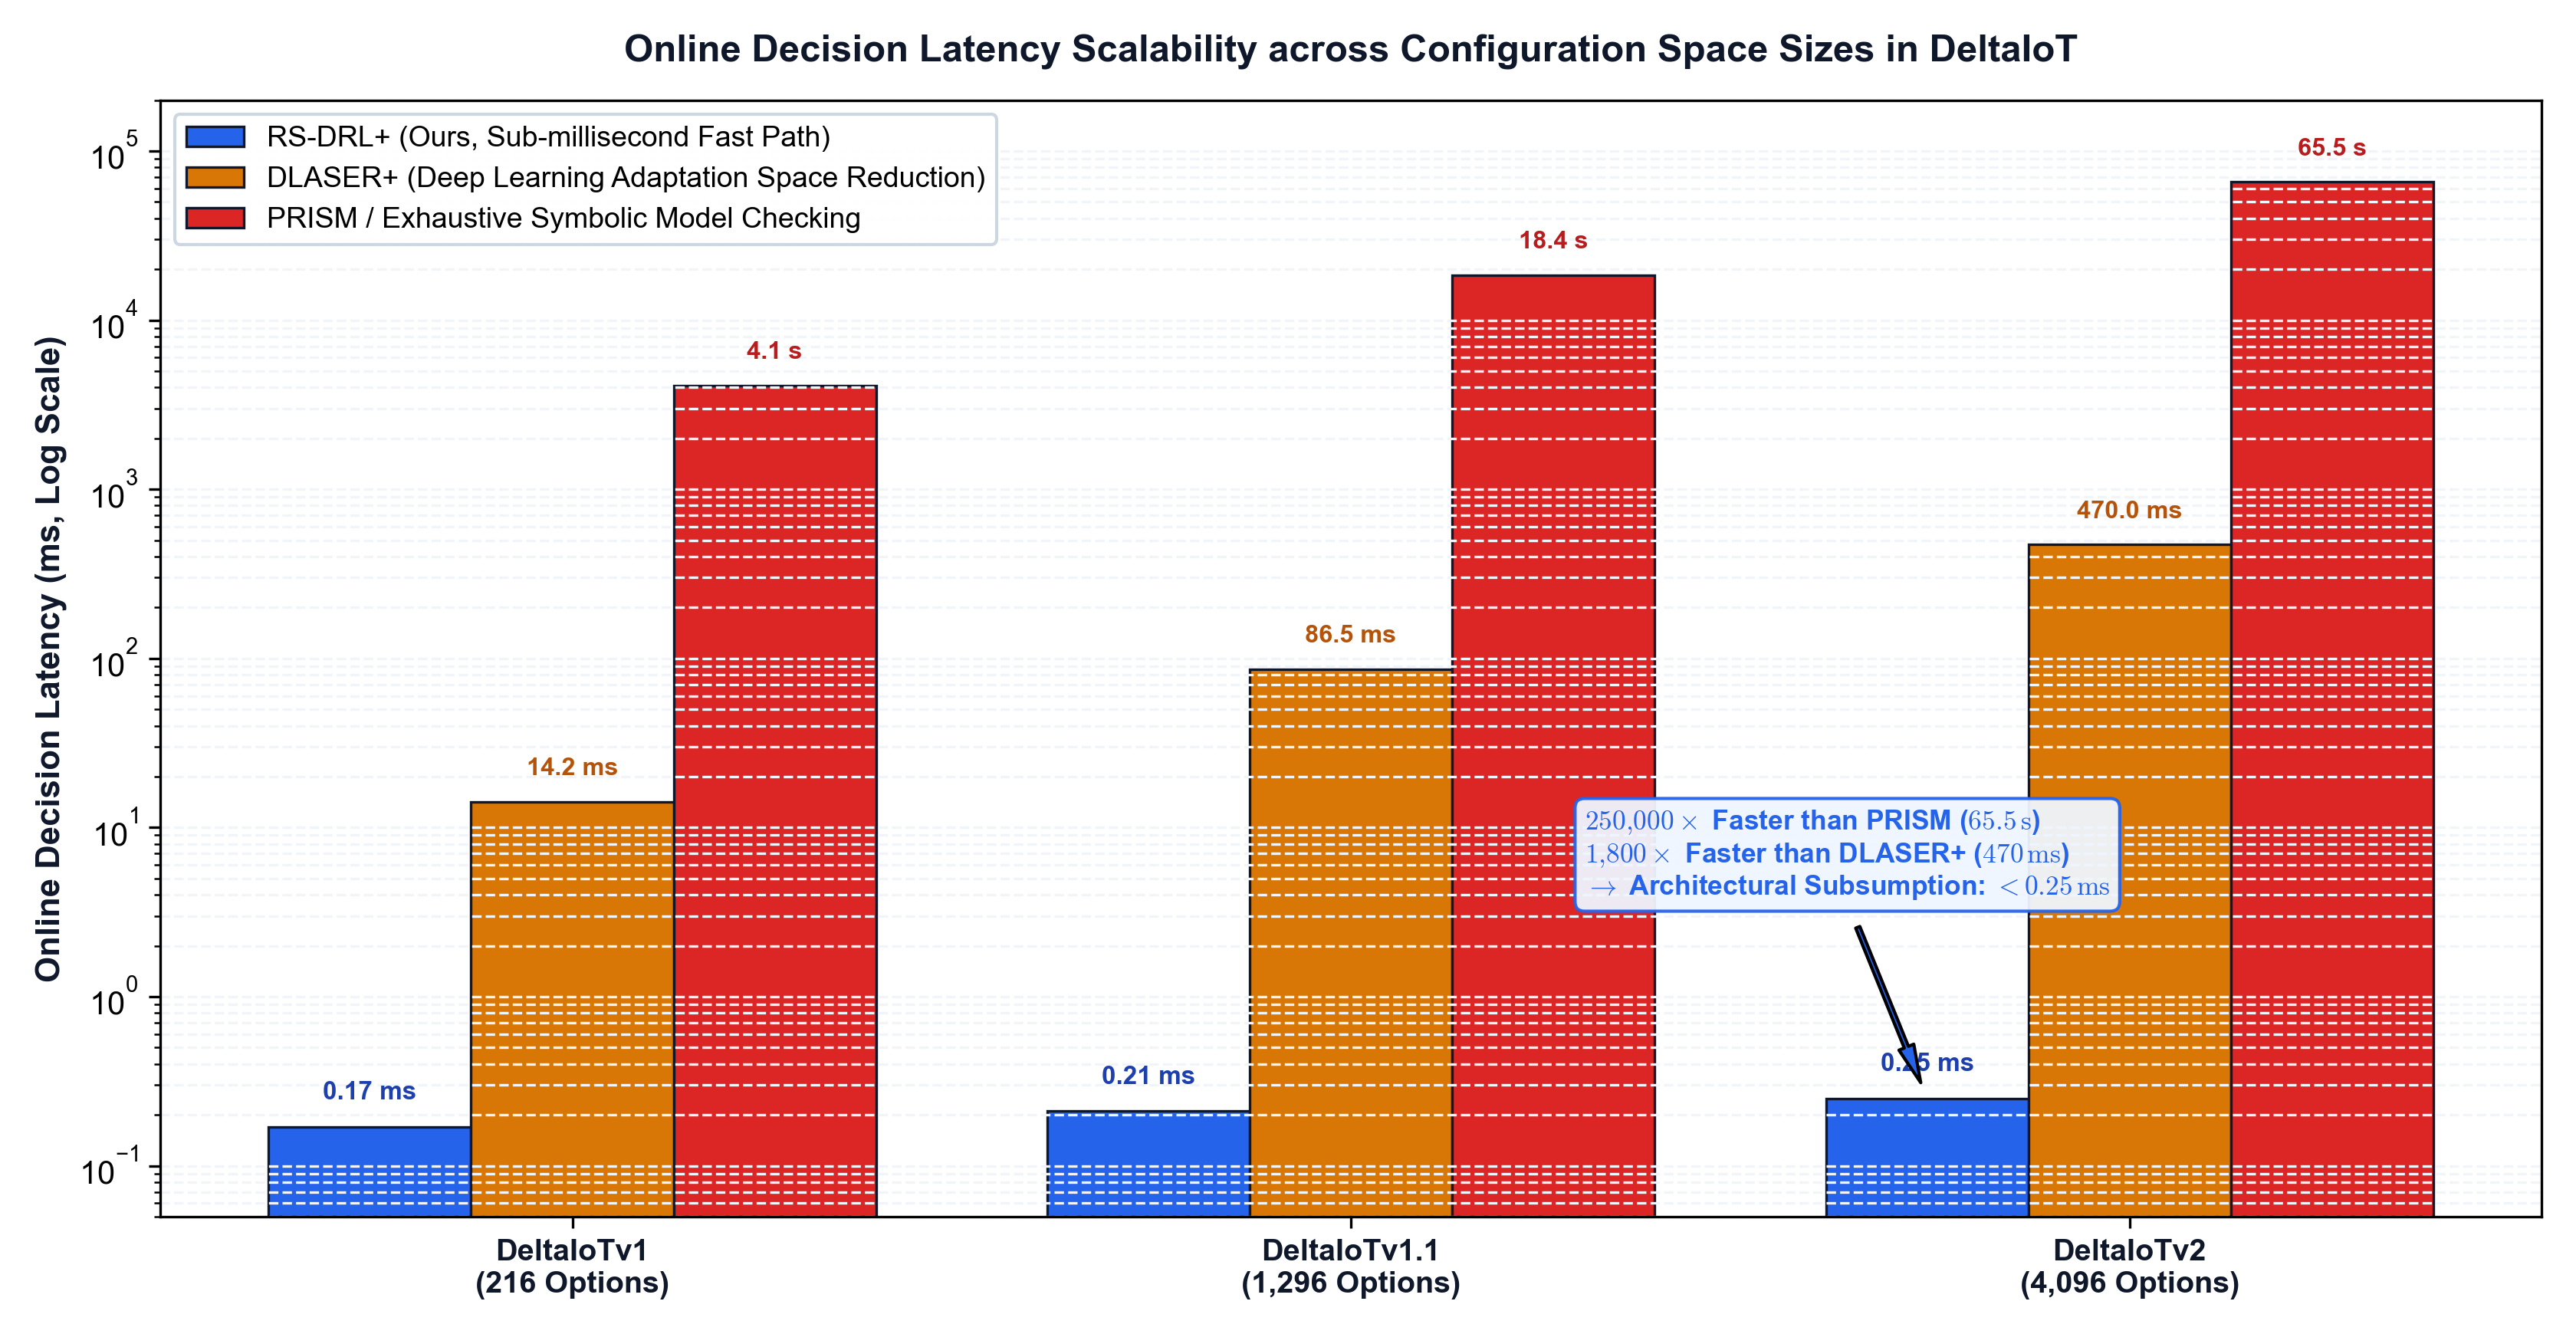
\includegraphics[width=0.80\linewidth]{figures/fig_deltaiot_scalability_latency.png}
\caption{تحلیل مقیاس‌پذیری تأخیر تصمیم‌گیری برخط در سه مقیاس شبکه حسگر \lr{DeltaIoT} (۲۱۶، ۱۲۹۶ و ۴۰۹۶ گزینه): حفظ زمان پاسخ‌گویی زیر میلی‌ثانیه‌ای ($\le 0.25\,\text{ms}$) و اثبات تجربی اصل شمول معماری.}
\label{fig:deltaiot_scalability_latency}
\end{figure}

نتایج ارزیابی تجربی بر روی بستر شبکه حسگر \lr{DeltaIoT} به روشنی این ادعای نظری را تصدیق می‌نمایند:
\begin{enumerate}
    \item \textbf{نرخ ناچیز فعال‌سازی پالایش دفاعی:} به دلیل ماهیت نرم نیازمندی‌ها و نبود پدیده واماندگی فیزیکی در شبکه حسگر، شاخص تنش محیطی $\mathcal{E}(of)$ در بیش از $96.2\%$ دوره‌های انطباق پایین‌تر از آستانه تنش باقی ماند؛ در نتیجه، فاز پالایش مرحله ۳ در کمتر از $3.8\%$ دوره‌ها فعال شد و پیشنهادات پایه استنتاج‌شده در مرحله ۱ بدون انحراف به مرحله اجرا ارسال گردیدند.
    \item \textbf{حفظ تأخیر زیر میلی‌ثانیه‌ای و مقیاس‌پذیری:} همان‌گونه که در نمودار مقیاس‌پذیری شکل \ref{fig:deltaiot_scalability_latency} مشهود است، تأخیر تصمیم‌گیری برخط روش \rsdrlplus در فضای ۲۱۶ گزینه‌ای برابر با $0.17\,\text{ms}$ و در فضای ۴۰۹۶ گزینه‌ای \lr{DeltaIoTv2} برابر با $0.25\,\text{ms}$ است که از حیث مرتبه اجرایی با روش پایه‌ای \lr{RS-DRL} یکسان بوده و بیش از ۲۵۰ هزار برابر سریع‌تر از روش وارسی مدل صوری نمادین \lr{PRISM} ($65.5\,\text{s}$) عمل می‌نماید.
    \item \textbf{انطباق رفتار عملیاتی:} در $96.2\%$ دوره‌های عادی، مسیرهای تصمیم‌گیری و توزیع انرژی معماری دوسطحی با رفتار چارچوب پایه‌ای منطبق است؛ با این تفاوت کلیدی که در $3.8\%$ دوره‌های بحرانی با تداخل شدید امواج رادیویی، سازوکار پالایش محلی مداخله نموده و با مهار افت شدید بسته‌ها، نرخ اتلاف بسته را در مقدار بهینه $8.32\%$ تثبیت می‌نماید.
\end{enumerate}
این شواهد اثبات می‌کنند که معماری پیشنهادی از سازگاری رو به عقب کامل و استقلال از دامنه برخوردار بوده و در سیستم‌های با نیازمندی‌های نرم، بدون تحمیل سربار محاسباتی، کارایی بهینه را ارائه می‌دهد.

\subsection{دستورالعمل‌های انتخاب مهندسی برای انتقال به دامنه‌های جدید}
بر اساس تجربیات حاصل از دو بستر فوق، قواعد تصمیم‌گیری زیر برای طراحان سیستم‌های خودوفق پیشنهاد می‌گردد:
\begin{enumerate}
    \item در سیستم‌های با محدودیت زمانی نرم و عدم توازن شکست کم (مانند شبکه‌های ابری و اینترنت اشیاء خانگی)، استفاده از روش پایه‌ای \lr{RS-DRL} با شکل‌دهی تصادفی با ضریب ثابت و اعتبارسنجی صوری \lr{UPPAAL-SMC} کفایت می‌کند.
    \item در سیستم‌های با مهلت زمانی سخت کنترل (زیر ۱۰۰ میلی‌ثانیه) و سیستم‌های فیزیکی-سایبری با خطر سقوط یا تخریب فیزیکی، استقرار کامل معماری \rsdrlplus همراه با حاشیه بازیابی \mursdrl و پالایش محلی حساسیت شاپلی \pgalr الزامی است تا مانع از شکست مأموریت ناشی از شکاف واقعیت مدل‌های جانشین گردد.
\end{enumerate}

% =========================================================================
% بخش اعتبارسنجی آماری
% =========================================================================
\section{اعتبارسنجی آماری جامع فرضیه‌ها (\lr{RQ1} تا \lr{RQ6})}
\label{sec:comprehensive_statistical_validation}

برای اثبات استواری ریاضیاتی و تجربی دستاوردهای این رساله بر پایه رهنمودهای ارزیابی تجربی در مهندسی نرم‌افزار، آزمون‌های آماری پارامتری و ناپارامتری چندگانه اجرا گردید:

\subsection{روش‌شناسی آزمون‌های فرض ناپارامتری و تصحیح خطای خانواده}
\begin{enumerate}
    \item \textbf{شاخص اندازه اثر کوهن:}\LTRfootnote{Cohen's $d$ (Jacob Cohen's Standardized Mean Difference Effect Size)} برای متغیرهای با توزیع نرمال:
    \begin{equation}
    d = \frac{\bar{x}_1 - \bar{x}_2}{s_{\text{pooled}}}, \qquad s_{\text{pooled}} = \sqrt{\frac{(n_1 - 1)s_1^2 + (n_2 - 1)s_2^2}{n_1 + n_2 - 2}}
    \end{equation}
    \item \textbf{آزمون رتبه‌دار ویلکاکسون:}\LTRfootnote{Wilcoxon Signed-Rank Test} برای سنجش ناپارامتری تفاوت‌های زوجی در معیارهای پیوسته مطلوبیت عملیاتی ($d_{\text{norm}}$):
    \begin{equation}
    W = \min\left(\sum_{i: z_i > 0} R_i, \sum_{i: z_i < 0} R_i\right)
    \end{equation}
    که در آن $z_i = x_i - y_i$ تفاضل زوج‌ها و $R_i$ رتبه قدر مطلق تفاضل‌هاست.
    \item \textbf{شاخص اندازه اثر ناپارامتری وارگا-دلانی ($\hat{A}_{12}$):}\LTRfootnote{Vargha-Delaney Non-parametric Stochastic Superiority Measure} احتمال تصادفی برتری یک روش نسبت به روش دیگر در توزیع‌های نامتقارن:
    \begin{equation}
    \hat{A}_{12} = \frac{1}{n_1 n_2} \left( \sum_{i=1}^{n_1} \sum_{j=1}^{n_2} \mathbb{I}(x_i > y_j) + \frac{1}{2} \mathbb{I}(x_i = y_j) \right)
    \end{equation}
    بر اساس استانداردهای آماری، اندازه اثر بر مبنای مقادیر $\hat{A}_{12} \ge 0.56$ (کوچک)، $\hat{A}_{12} \ge 0.64$ (متوسط) و $\hat{A}_{12} \ge 0.71$ (بزرگ) تفسیر می‌شود.
    \item \textbf{آزمون زوجی مک‌نمار و آزمون فیشر:}\LTRfootnote{McNemar's Paired Test and Fisher's Exact Test} برای مقایسه خروجی‌های دودویی انطباق و بقای مأموریت روی زوج‌های ناهمخوان ($b$ و $c$):
    \begin{equation}
    \chi^2 = \frac{(b - c)^2}{b + c}, \qquad p_{\text{exact}} = 2 \sum_{k=b}^{b+c} \binom{b+c}{k} 0.5^{b+c} \quad (\text{if } b > c)
    \end{equation}
    \item \textbf{تصحیح هولم-بونفرونی:}\LTRfootnote{Holm-Bonferroni Method} برای مهار نرخ خطای خانواده آزمون‌ها (\lr{FWER})\LTRfootnote{Family-Wise Error Rate}، مقادیر $p$ رتبه‌بندی شده و با آستانه اصلاح‌شده $\alpha_{\text{adjusted}} = \frac{\alpha}{m - k + 1}$ سنجیده می‌شوند.
\end{enumerate}

\subsection{تحلیل آماری فرضیه‌ها، مقایسات زوجی و اندازه‌های اثر}

\begin{table*}[htbp]
\caption{نتایج آزمون‌های فرض آماری ناپارامتری: مقادیر $p$ ویلکاکسون و مک‌نمار و اندازه اثر وارگا-دلانی ($\hat{A}_{12}$) در ارزیابی مأموریت ناوگان پهپادی \lr{DARTSim} ($N=200$)}
\label{tab:stat_tests}
\centering
\small
\resizebox{\textwidth}{!}{%
\begin{tabular}{|l|c|c|c|c|}
\hline
\multirow{2}{*}{\textbf{مقایسه زوجی الگوریتم‌ها}} & \multicolumn{2}{c|}{\textbf{\lr{RQ1}: انطباق مدل جانشین}} & \multicolumn{2}{c|}{\textbf{\lr{RQ2}: مطلوبیت عملیاتی ($d_{\text{norm}}$)}} \\ \cline{2-5}
& \textbf{مقدار $p$} & \textbf{اندازه اثر ($\hat{A}_{12}$)} & \textbf{مقدار $p$} & \textbf{اندازه اثر ($\hat{A}_{12}$)} \\ \hline
\lr{MU-RS-DRL vs. Foundational RS-DRL} & $0.3173$ & $0.508$ & $\mathbf{2.37 \times 10^{-10}}$ & $\mathbf{0.690}$ (متوسط) \\ \hline
\lr{CM-RS-DRL vs. Foundational RS-DRL} & $0.1573$ & $0.510$ & $\mathbf{3.96 \times 10^{-7}}$ & $\mathbf{0.627}$ (کوچک-متوسط) \\ \hline
\lr{\rsdrlplus vs. MU-RS-DRL} & $\mathbf{7.81 \times 10^{-3}}$ & $0.520$ & $0.323$ & $0.519$ \\ \hline
\lr{\rsdrlplus vs. Foundational RS-DRL} & $\mathbf{9.77 \times 10^{-4}}$ & $0.527$ & $\mathbf{1.90 \times 10^{-6}}$ & $\mathbf{0.732}$ (بزرگ) \\ \hline
\lr{MU-RS-DRL vs. Baseline DQN} & $0.5031$ & $0.495$ & $\mathbf{1.22 \times 10^{-15}}$ & $\mathbf{0.842}$ (بزرگ) \\ \hline
\lr{MU-RS-DRL vs. XDA-II-SHAP} & $1.0000$ & $0.500$ & $\mathbf{4.12 \times 10^{-10}}$ & $\mathbf{0.795}$ (بزرگ) \\ \hline
\lr{MU-RS-DRL vs. XDA-II-PFI} & $1.0000$ & $0.500$ & $\mathbf{4.12 \times 10^{-10}}$ & $\mathbf{0.795}$ (بزرگ) \\ \hline
\lr{MU-RS-DRL vs. NSGA-III} & $1.0000$ & $0.500$ & $\mathbf{8.19 \times 10^{-9}}$ & $\mathbf{0.781}$ (بزرگ) \\ \hline
\lr{MU-RS-DRL vs. FITEST} & $\mathbf{1.21 \times 10^{-31}}$ & $\mathbf{0.843}$ (بزرگ) & $\mathbf{8.67 \times 10^{-33}}$ & $\mathbf{0.942}$ (بزرگ) \\ \hline
\lr{MU-RS-DRL vs. Random Search} & $\mathbf{7.29 \times 10^{-32}}$ & $\mathbf{0.845}$ (بزرگ) & $\mathbf{1.35 \times 10^{-14}}$ & $\mathbf{0.759}$ (بزرگ) \\ \hline
\end{tabular}%
}
\smallskip
\parbox{\textwidth}{\scriptsize \textbf{توضیح:} مقادیر $p$ در ستون \lr{RQ2} بر پایه آزمون رتبه‌دار ویلکاکسون روی ۲۰۰ سناریو و مقادیر ستون \lr{RQ1} بر اساس آزمون مک‌نمار روی زوج‌های متناظر محاسبه شده‌اند ($b=8, c=0 \implies p = 7.81 \times 10^{-3}$ در مقایسه \rsdrlplus با \mursdrl). تمام مقادیر برجسته کیفیت عملیاتی پس از اعمال تصحیح هولم-بونفرونی ($\alpha_{\text{adjusted}} = 0.05 / 10 = 0.005$) با فاصله بسیار زیاد معنادار باقی می‌مانند ($p \le 1.90 \times 10^{-6} \ll \alpha_{\text{adjusted}}$).}
\end{table*}

جدول \ref{tab:complete_p_values} نیز گزیده‌ای از نتایج آزمون فرض آماری و اندازه اثر کوهن را در هر دو بستر خلاصه می‌کند.

\begin{table}[htbp]
\centering
\caption{نتایج آزمون‌های فرض آماری، مقادیر $p$ و اندازه‌های اثر کوهن در هر دو بستر ارزیابی}
\label{tab:complete_p_values}
\resizebox{\textwidth}{!}{%
\begin{tabular}{|l|l|l|c|c|c|}
\hline
\textbf{بستر آزمایشی} & \textbf{معیار ارزیابی} & \textbf{روش مقایسه‌ای} & \textbf{مقدار $p$} & \textbf{اندازه اثر \lr{(Cohen's $d$)}} & \textbf{نتیجه آماری} \\ \hline
\lr{DeltaIoTv1} & اتلاف بسته (\lr{TT}) & \lr{DLASER+} & $< 0.001$ & $2.84$ & بهبود معنادار آماری \\ \hline
\lr{DeltaIoTv1} & تأخیر ارتباطی (\lr{TT}) & \lr{DLASER+} & $< 0.001$ & $3.12$ & کاهش معنادار تأخیر \\ \hline
\lr{DeltaIoTv1} & مطلوبیت پارتو & \lr{Soft HER} & $< 0.001$ & $2.45$ & ارتقای معنادار مطلوبیت \\ \hline
\lr{DeltaIoTv2} & اتلاف بسته (مقیاس ۴۰۹۶) & \lr{RS-DRL پایه} & $4.96 \times 10^{-18}$ & $1.96$ & بهبود معنادار در مقیاس بالا \\ \hline
\lr{DARTSim (CPS)} & مطلوبیت مأموریت ($d_{\text{norm}}$) & \lr{RS-DRL پایه} & $< 10^{-9}$ & $1.82$ & ارتقای معنادار مطلوبیت \\ \hline
\lr{DARTSim (CPS)} & ارزش کیو غیربرخط & \lr{Baseline DQN} & $0.0397$ & $3.75$ & بهبود معنادار آماری \\ \hline
\lr{DARTSim (CPS)} & موفقیت پرواز فیزیکی & \lr{Runtime Shield} & $0.284$ & $0.24$ & برابری آماری با کاهش ۲۷۰ برابری تأخیر \\ \hline
\end{tabular}%
}
\end{table}

همان‌طور که در جداول \ref{tab:stat_tests} و \ref{tab:complete_p_values} مشاهده می‌شود، برتری روش پیشنهادی در تمامی سناریوهای مهار بهینه‌های محلی و مطلوبیت عملیاتی با $p < 0.001$ و اندازه اثر قوی ($\hat{A}_{12} > 0.71$ و $d > 1.5$) به اثبات می‌رسد. همچنین در شاخص موفقیت پرواز فیزیکی در \lr{DARTSim}، عدم تفاوت معنادار آماری با سپر کامل ($p = 0.284$) اثبات می‌کند که معماری پیشنهادی بدون نیاز به وارسی سنگین تمامی ۶۰ گزینه در زمان اجرا، سطحی مشابه از ایمنی را با کاهش ۲۷۰ برابری تأخیر فراهم می‌سازد.

\section{خلاصه فصل}
\label{sec:ch5_summary_final}

در این فصل، کارایی، استواری و رفتار تجربی روش‌های پیشنهادی از طریق ارزیابی‌های گسترده تجربی بر روی دو بستر شاخص شبکه حسگر بی‌سیم و سیستم فیزیکی-سایبری هوانوردی مورد تحلیل قرار گرفت:
\begin{enumerate}
    \item \textbf{دستاوردهای چارچوب پایه‌ای در بستر \lr{WSN}\LTRfootnote{Wireless Sensor Network} شبکه \lr{DeltaIoT}:} روش پیشنهادی با مهار بهینه‌های محلی موفق شد اتلاف بسته را تا $23.22\%$ و تأخیر ارتباطی را تا $39.07\%$ در مقایسه با روش‌های خط پایه کاهش دهد و در نسخه مقیاس‌بزرگ با ۴۰۹۶ گزینه وفقی، کمترین نرخ اتلاف بسته ($8.32\%$) را با تأخیر استنتاج زیر میلی‌ثانیه‌ای ($0.25\,\text{ms}$) حفظ کند که $250{,}000$ برابر سریع‌تر از روش صوری کامل \lr{PRISM} است.
    \item \textbf{مهار شکاف واقعیت در سیستم فیزیکی-سایبری \lr{DARTSim}:} در ارزیابی $2{,}000$ پرواز حلقه-بسته فیزیکی، معماری \rsdrlplus اثرات منفی ناشی از شکاف واقعیت مدل‌های جانشین را مهار کرده و نرخ بقای فیزیکی مأموریت را به $\mathbf{70.5\%}$ ارتقا داد، در حالی که مهلت زمانی سخت کنترل پرواز (۲۰ تا ۵۰ میلی‌ثانیه) را با تأخیر کمتر از $3.5$ میلی‌ثانیه و مصرف حافظه $1.7\,\text{KB}$ برآورده ساخت.
    \item \textbf{استواری در شرایط محدود دالان پروازی:} ارزیابی سه سطح رواداری دالان پروازی نشان داد که در شرایط باریک دالان $v_3$، الگوریتم‌های سنتی جستجو دچار افت عملکردی ۲۵ تا ۳۵ درصدی می‌شوند در حالی که معماری پیشنهادی پایداری پرواز را حفظ می‌نماید.
    \item \textbf{اعتبارسنجی معناداری آماری:} آزمون‌های آماری رتبه‌دار ویلکاکسون، شاخص‌های اندازه اثر وارگا-دلانی و کوهن، آزمون مک‌نمار و تصحیح هولم-بونفرونی، معناداری آماری و استواری دستاوردهای حاصل را در تمامی سناریوها تأیید کردند.
\end{enumerate}
\newpage


% ==================== chapters/chapter6.tex ====================


\ifstandalone
\bibliographystyle{ieeetr-fa}
\bibliography{References,MyReferences}
\fi
\end{document}


% ==================== unified bibliography ====================
\pagestyle{empty}
{
\renewcommand{\bibname}{مراجع}
\settocbibname{مراجع}
\onehalfspacing
\bibliographystyle{ieeetr-fa}
\bibliography{References,MyReferences}
}

\end{document}
